\documentclass[a4paper,12pt]{scrartcl} 

%Beginn Präambel
\usepackage[english]{babel} %Deutsche Einstelungen
\usepackage[utf8]{inputenc} %utf-8 Eingabe
\usepackage[T1]{fontenc} % Korrekte Aufgabefonds im Aufabedokument
\usepackage{csquotes} %Anführungsstriche mit \enquote{text}
\linespread{1.3}
\usepackage{amsmath}
\usepackage{color}
\usepackage{caption}
\usepackage{booktabs}
\usepackage{graphicx}
\graphicspath{{Graphen/}}
\usepackage{siunitx}
\sisetup{locale = US}
\usepackage{placeins}
\usepackage[version=4,arrows=pgf]{mhchem}
\usepackage{float}
\usepackage[backend=biber,style=chem-angew,sorting=none]{biblatex}
\addbibresource{literatur.bib}
\usepackage{blindtext}
\setcounter{secnumdepth}{3}
\setcounter{tocdepth}{2}
\usepackage[a4paper, lmargin={2cm}, rmargin={2cm}, tmargin={2cm}, bmargin={2cm}]{geometry}
\usepackage{url}
\usepackage{hyperref}
\usepackage[all]{hypcap}
\hypersetup{pdfstartview=FitH, pdfauthor=Tom Frömbgen}
\usepackage{fancyhdr}
%\setlength{\skip\footins}{3mm}
\pagestyle{fancy}
\fancyhf{}
\fancyhead[L]{WP 12}
\fancyhead[C]{Theoretical Methods for Condensed Matter}
\fancyhead[R]{Tom Frömbgen}
\fancyfoot[R]{\thepage}



% Neue Kommandos
\newcommand{\tb}{\textbackslash}
\newcommand{\tf}{\textbf}
\newcommand{\x}{\chi}
\newcommand{\xm}{\chi_ \m{M}}
\newcommand{\dxm}{\Delta\chi_\m{M}}
%\newcommand{\chapref}[1]{Chapter~\ref{#1}}
%\newcommand{\secref}[1]{Section~\ref{#1}}
%\newcommand{\tabref}[1]{Table~\ref{#1}}
%\newcommand{\figref}[1]{Figure~\ref{#1}}
\newcommand{\m}[1]{\mathrm{#1}}
\renewcommand{\arraystretch}{1.0}
\newcommand{\leadingzero}[1]{\ifnum #1<10 0\the#1\else\the#1\fi}
\newcommand{\euler}{\m{e}}
\newcommand{\imag}{\m{i}}
\newcommand{\nt}{\noindent}
\newcommand{\sub}{\textsubscript}
\newcommand{\super}{\textsuperscript}


\begin{document}
%
\thispagestyle{empty}

%
\begin{center}
	\begin{LARGE}
		\vspace{50mm}
		\textbf{WP12} \\
		\vspace{15mm}
		\textbf{Theoretical Methods for Condensed Matter} \\
		\vspace{15mm}
		\textbf{Part I} \\
		\vspace{30mm}
	\end{LARGE}
	\begin{large}
		Tom Frömbgen \\
		\vspace{20mm}
		Assistants: Shima Taherivardanjani \& Henrik Niemöller  \\
		\vspace{10mm}
		Submission 1: \today \\
		\vspace{5mm}
%		Submission 2:  \today
	\end{large}
\end{center}

%
%\newpage
%\thispagestyle{empty}
%\tableofcontents
\newpage
%
\section{Introduction}
%
	This course focuses on Molecular Dynamics (MD). The underlying theory was explained during the lecture. To gain further insights into the topic of MD, simulations of water which is the most important liquid in humans' life were to be performed. Although the \ce{H2O} molecule is rather simple, simulations of liquid water require large effort to describe the inter- and intramolecular interactions accurately. There are different approaches to face this challenge ranging from \emph{ab initio} quantum chemical methods to (semi) empirical force fields.
	
	Herein, three different force fields that were especially developed for water and the results of their application are presented: 
	\begin{enumerate}
		\item The extended simple point charge water model SPC/E\autocite{berendsen1987missing} is a rigid, three-site effective pair potential. The three sites which are located at the positions of hydrogen and oxygen atoms carry point charges. Non-bonded interactions are described for oxygen-oxygen pairs exclusively, via a Lennard-Jones potential. Due to its rigidness this model allows for a large time step and thus fast computation since the fastest motions of this system which limit the time step of the simulation are librational movements around hydrogen bonds.
		
		\item The flexible simple point charge water model SPC/Fw\autocite{wu2006flexible} is a flexible, three-site effective pair potential which contains point charges on the interaction sites that are located on the hydrogen and oxygen atoms. Again, non-bonded interactions are described for oxygen-oxygen pairs exclusively via a Lennard-Jones potential. In contrast to the model presented before, SPC/Fw describes water not as rigid but with flexibility regarding bond stretching and angle bending. Accordingly this results in a smaller time step and higher computational costs.
		
		\item The SPC-FQ\autocite{rick1994dynamical} water model is a rigid, three-site, polarizable water model. This model tries to make an improvement compared to SPC/E by introducing many-body effects in the form of electric polarization. The charges are not fixed but can adapt to fluctuations of the electric field caused by the interactions with other molecules. The improvement of the charge description comes with a drastic increase in computational demand since special algorithms are needed to solve the equations of the electric field.
	\end{enumerate}

	
	
%
\section{Computational Details}
%
	Three simulations of liquid water employing the force fields SPC/E, SPC/Fw and SPC-FQ were performed using the \textsc{Lammps}\autocite{plimpton1995fast} program package. In each of these, 512 water molecules were simulated in a cubic box ($ a = \SI{24.86}{\angstrom} $) with periodic boundary conditions. The chosen length of the box edge reflects the experimental density of water (see \autoref{tab:parameters}). The temperature was controlled by a Nos\'{e}--Hoover thermostat\autocite{nose1984unified,nose1984molecular}  ($T = \SI{298.15}{\kelvin},~ \tau=\SI{100}{\femto\second}$). The SHAKE\autocite{ryckaert1977numerical} algorithm was used. The cutoff radius for Lennard--Jones interactions was chosen as \linebreak $ r_C = \SI{11.0}{\angstrom} $. Coulomb interactions beyond this cutoff radius were computed by usage of the particle-particle particle mesh solver\autocite{hockney1988computer} with an accuracy of $10^{-5}$. The time step was chosen as $ \delta t=\SI{1.0}{\femto\second} $. An initial configuration was with random velocities was generated. After a melting of $ \SI{2}{\pico\sec} $ an equilibration run of $ \SI{100}{\pico\second} $ was performed, subsequently production runs of  $ \SI{100}{\pico\second} $ and $ \SI{1}{\nano\second} $ were performed with high and low dumping frequency, respectively. The force field parameters are depicted in \autoref{tab:parameters}. The obtained trajectories were analyzed with \textsc{Travis}\autocite{brehm2011travis,brehm2020travis}.
	%
	\begin{table}
		\centering
		\captionabove{Parameters of the water models SPC/E, SPC/Fw SPC-FQ: O--H stretching force constant $ k_b $ (in $ \SI{}{\frac{kcal}{\mole\cdot\angstrom^2}} $), O--H reference bond length $ r_0 $ (in $ \SI{}{\angstrom} $), H--O--H bending force constant $ k_a $ (in $ \SI{}{\frac{kcal}{\mole\cdot\radian^2}} $), H--O--H reference angle $ \alpha_0 $ (in $ \SI{}{deg} $), Lennard--Jones well depth  $ \varepsilon $ (in $ \SI{}{\frac{kcal}{\mole}} $) and diameter $ \sigma $ (in $ \SI{}{\angstrom} $), charges of the oxygen and hydrogen atoms $ q_O,~q_H $ (in $ e $) and density $ \rho $ (in $ \SI{}{\frac{\kilogram}{\deci\meter^3}} $).  }
		\label{tab:parameters}
		\begin{tabular}{c|ccccccccc}
			\toprule
			& $ k_b $ & $ r_0 $ & $ k_a $ & $ \alpha_0 $ & $ \varepsilon $ & $ \sigma $ & $ q_O $ & $q_H $ & $ \rho $ \\ 
			\midrule
			SPC/E & $ \infty $ & 1.000 & $ \infty $ & 109.47 & 0.1553 & 3.166 & -0.8476 & 0.4238 & 0.997\\
			SPC/Fw & 529.58 & 1.012 & 37.95 & 113.24 & 0.1554 & 3.165 & -0.8200 & -0.4100 & 0.997 \\
			SPC-FQ & $\infty $ & 1.000 & $ \infty $ & 109.47 & 0.2941 & 3.176 & -0.8200 & 0.4100 & 0.997\\
			\bottomrule
		\end{tabular}
	\end{table}
%
\section{Results and Discussion}		
%	
	\subsection{Radial Distribution Functions}
	%
		To gain a first insight into a simulation (after the visual inspection of the trajectories), radial distribution functions (RDFs) provide important information about the interactions in the simulated system. A RDF of A--B displays the probability $ g(r) $ to find a defined particle B at distance $ r $ away from another defined particle A. Oxygen-oxygen as well as oxygen-hydrogen RDFs have been computed. The latter ones refer to O--H pairs where O and H are not part of the same molecule. 
		
		As can be seen in \autoref{fig:rdf}, first maxima of the O--O RDFs are at larger distance compared to the O--H RDFs throughout all three investigated force fields. The position of the first maximum refers to the average distance between the respective atoms. This observation  is reasonable since oxygen and hydrogen atoms are oppositely charged and thereby attract each other, whereas oxygen atoms repulse each other. Noting the tendency of water molecules to form hydrogen bonds, the position of the first maximum can be assigned to the average length of a hydrogen bond. Analogously, the RDFs' first minima represent the extent of the first solvation shell. Again, this distances are larger for the O--O atom pairs than for the O--H atom pairs.
		
		Comparing the three models, it is observed that SPC/E and SPC/Fw show similar results with respect to the RDFs. Opposed to that, the simulation with SPC-FQ as a model shows first maxima and minima that are shifted to increased distances which can be deduced to the fact that SPC-FQ is a more repulsive model. This force field allows for charge distribution according to the environment of a molecule. Vice versa, SPC/E and SPC/Fw describe electrostatic interactions by point charges only. Since the charges are more located (or in a way more \enquote{concentrated} / less diffuse) in SPC/E and SPC/Fw, sharper and higher peaks at smaller distances are observed in the RDFs.
		
		Furthermore, the first maximum of the O--H RDF of SPC-FQ shows an unexpectedly small value: $ g(r_\m{max}) < 1 $. Additionally the second maximum shows an exceptionally high peak compared to the first one. This indicates that the number of particles in the first solvation shell is rather low, compared to the second one. This behavior is not observed for SPC/E and SPC/Fw, but exactly the other way around. The first peak in the O--H RDF represents the commonly known water hydrogen bonds, the second peak summarizes all other hydrogen-oxygen interactions.
		
		Comparison of the obtained results with X-ray scattering\autocite{hura2000high} and neutron diffraction\autocite{soper2000radial} experiments proves the SPC/E and SPC/Fw models to yield reasonable results whereas SPC/FQ does not display the interactions between water molecules correctly w.r.t the RDFs.
		
		\begin{figure}
			\centering
			%% Creator: Matplotlib, PGF backend
%%
%% To include the figure in your LaTeX document, write
%%   \input{<filename>.pgf}
%%
%% Make sure the required packages are loaded in your preamble
%%   \usepackage{pgf}
%%
%% Figures using additional raster images can only be included by \input if
%% they are in the same directory as the main LaTeX file. For loading figures
%% from other directories you can use the `import` package
%%   \usepackage{import}
%% and then include the figures with
%%   \import{<path to file>}{<filename>.pgf}
%%
%% Matplotlib used the following preamble
%%   \usepackage{amssymb} \usepackage{amsmath}
%%
\begingroup%
\makeatletter%
\begin{pgfpicture}%
\pgfpathrectangle{\pgfpointorigin}{\pgfqpoint{6.694230in}{4.016538in}}%
\pgfusepath{use as bounding box, clip}%
\begin{pgfscope}%
\pgfsetbuttcap%
\pgfsetmiterjoin%
\definecolor{currentfill}{rgb}{1.000000,1.000000,1.000000}%
\pgfsetfillcolor{currentfill}%
\pgfsetlinewidth{0.000000pt}%
\definecolor{currentstroke}{rgb}{1.000000,1.000000,1.000000}%
\pgfsetstrokecolor{currentstroke}%
\pgfsetdash{}{0pt}%
\pgfpathmoveto{\pgfqpoint{0.000000in}{0.000000in}}%
\pgfpathlineto{\pgfqpoint{6.694230in}{0.000000in}}%
\pgfpathlineto{\pgfqpoint{6.694230in}{4.016538in}}%
\pgfpathlineto{\pgfqpoint{0.000000in}{4.016538in}}%
\pgfpathclose%
\pgfusepath{fill}%
\end{pgfscope}%
\begin{pgfscope}%
\pgfsetbuttcap%
\pgfsetmiterjoin%
\definecolor{currentfill}{rgb}{1.000000,1.000000,1.000000}%
\pgfsetfillcolor{currentfill}%
\pgfsetlinewidth{0.000000pt}%
\definecolor{currentstroke}{rgb}{0.000000,0.000000,0.000000}%
\pgfsetstrokecolor{currentstroke}%
\pgfsetstrokeopacity{0.000000}%
\pgfsetdash{}{0pt}%
\pgfpathmoveto{\pgfqpoint{0.592518in}{0.525000in}}%
\pgfpathlineto{\pgfqpoint{3.124543in}{0.525000in}}%
\pgfpathlineto{\pgfqpoint{3.124543in}{3.831538in}}%
\pgfpathlineto{\pgfqpoint{0.592518in}{3.831538in}}%
\pgfpathclose%
\pgfusepath{fill}%
\end{pgfscope}%
\begin{pgfscope}%
\pgfsetbuttcap%
\pgfsetroundjoin%
\definecolor{currentfill}{rgb}{0.000000,0.000000,0.000000}%
\pgfsetfillcolor{currentfill}%
\pgfsetlinewidth{0.803000pt}%
\definecolor{currentstroke}{rgb}{0.000000,0.000000,0.000000}%
\pgfsetstrokecolor{currentstroke}%
\pgfsetdash{}{0pt}%
\pgfsys@defobject{currentmarker}{\pgfqpoint{0.000000in}{-0.048611in}}{\pgfqpoint{0.000000in}{0.000000in}}{%
\pgfpathmoveto{\pgfqpoint{0.000000in}{0.000000in}}%
\pgfpathlineto{\pgfqpoint{0.000000in}{-0.048611in}}%
\pgfusepath{stroke,fill}%
}%
\begin{pgfscope}%
\pgfsys@transformshift{0.592518in}{0.525000in}%
\pgfsys@useobject{currentmarker}{}%
\end{pgfscope}%
\end{pgfscope}%
\begin{pgfscope}%
\pgftext[x=0.592518in,y=0.427778in,,top]{\rmfamily\fontsize{8.000000}{9.600000}\selectfont \(\displaystyle 0\)}%
\end{pgfscope}%
\begin{pgfscope}%
\pgfsetbuttcap%
\pgfsetroundjoin%
\definecolor{currentfill}{rgb}{0.000000,0.000000,0.000000}%
\pgfsetfillcolor{currentfill}%
\pgfsetlinewidth{0.803000pt}%
\definecolor{currentstroke}{rgb}{0.000000,0.000000,0.000000}%
\pgfsetstrokecolor{currentstroke}%
\pgfsetdash{}{0pt}%
\pgfsys@defobject{currentmarker}{\pgfqpoint{0.000000in}{-0.048611in}}{\pgfqpoint{0.000000in}{0.000000in}}{%
\pgfpathmoveto{\pgfqpoint{0.000000in}{0.000000in}}%
\pgfpathlineto{\pgfqpoint{0.000000in}{-0.048611in}}%
\pgfusepath{stroke,fill}%
}%
\begin{pgfscope}%
\pgfsys@transformshift{1.014522in}{0.525000in}%
\pgfsys@useobject{currentmarker}{}%
\end{pgfscope}%
\end{pgfscope}%
\begin{pgfscope}%
\pgftext[x=1.014522in,y=0.427778in,,top]{\rmfamily\fontsize{8.000000}{9.600000}\selectfont \(\displaystyle 200\)}%
\end{pgfscope}%
\begin{pgfscope}%
\pgfsetbuttcap%
\pgfsetroundjoin%
\definecolor{currentfill}{rgb}{0.000000,0.000000,0.000000}%
\pgfsetfillcolor{currentfill}%
\pgfsetlinewidth{0.803000pt}%
\definecolor{currentstroke}{rgb}{0.000000,0.000000,0.000000}%
\pgfsetstrokecolor{currentstroke}%
\pgfsetdash{}{0pt}%
\pgfsys@defobject{currentmarker}{\pgfqpoint{0.000000in}{-0.048611in}}{\pgfqpoint{0.000000in}{0.000000in}}{%
\pgfpathmoveto{\pgfqpoint{0.000000in}{0.000000in}}%
\pgfpathlineto{\pgfqpoint{0.000000in}{-0.048611in}}%
\pgfusepath{stroke,fill}%
}%
\begin{pgfscope}%
\pgfsys@transformshift{1.436526in}{0.525000in}%
\pgfsys@useobject{currentmarker}{}%
\end{pgfscope}%
\end{pgfscope}%
\begin{pgfscope}%
\pgftext[x=1.436526in,y=0.427778in,,top]{\rmfamily\fontsize{8.000000}{9.600000}\selectfont \(\displaystyle 400\)}%
\end{pgfscope}%
\begin{pgfscope}%
\pgfsetbuttcap%
\pgfsetroundjoin%
\definecolor{currentfill}{rgb}{0.000000,0.000000,0.000000}%
\pgfsetfillcolor{currentfill}%
\pgfsetlinewidth{0.803000pt}%
\definecolor{currentstroke}{rgb}{0.000000,0.000000,0.000000}%
\pgfsetstrokecolor{currentstroke}%
\pgfsetdash{}{0pt}%
\pgfsys@defobject{currentmarker}{\pgfqpoint{0.000000in}{-0.048611in}}{\pgfqpoint{0.000000in}{0.000000in}}{%
\pgfpathmoveto{\pgfqpoint{0.000000in}{0.000000in}}%
\pgfpathlineto{\pgfqpoint{0.000000in}{-0.048611in}}%
\pgfusepath{stroke,fill}%
}%
\begin{pgfscope}%
\pgfsys@transformshift{1.858531in}{0.525000in}%
\pgfsys@useobject{currentmarker}{}%
\end{pgfscope}%
\end{pgfscope}%
\begin{pgfscope}%
\pgftext[x=1.858531in,y=0.427778in,,top]{\rmfamily\fontsize{8.000000}{9.600000}\selectfont \(\displaystyle 600\)}%
\end{pgfscope}%
\begin{pgfscope}%
\pgfsetbuttcap%
\pgfsetroundjoin%
\definecolor{currentfill}{rgb}{0.000000,0.000000,0.000000}%
\pgfsetfillcolor{currentfill}%
\pgfsetlinewidth{0.803000pt}%
\definecolor{currentstroke}{rgb}{0.000000,0.000000,0.000000}%
\pgfsetstrokecolor{currentstroke}%
\pgfsetdash{}{0pt}%
\pgfsys@defobject{currentmarker}{\pgfqpoint{0.000000in}{-0.048611in}}{\pgfqpoint{0.000000in}{0.000000in}}{%
\pgfpathmoveto{\pgfqpoint{0.000000in}{0.000000in}}%
\pgfpathlineto{\pgfqpoint{0.000000in}{-0.048611in}}%
\pgfusepath{stroke,fill}%
}%
\begin{pgfscope}%
\pgfsys@transformshift{2.280535in}{0.525000in}%
\pgfsys@useobject{currentmarker}{}%
\end{pgfscope}%
\end{pgfscope}%
\begin{pgfscope}%
\pgftext[x=2.280535in,y=0.427778in,,top]{\rmfamily\fontsize{8.000000}{9.600000}\selectfont \(\displaystyle 800\)}%
\end{pgfscope}%
\begin{pgfscope}%
\pgfsetbuttcap%
\pgfsetroundjoin%
\definecolor{currentfill}{rgb}{0.000000,0.000000,0.000000}%
\pgfsetfillcolor{currentfill}%
\pgfsetlinewidth{0.803000pt}%
\definecolor{currentstroke}{rgb}{0.000000,0.000000,0.000000}%
\pgfsetstrokecolor{currentstroke}%
\pgfsetdash{}{0pt}%
\pgfsys@defobject{currentmarker}{\pgfqpoint{0.000000in}{-0.048611in}}{\pgfqpoint{0.000000in}{0.000000in}}{%
\pgfpathmoveto{\pgfqpoint{0.000000in}{0.000000in}}%
\pgfpathlineto{\pgfqpoint{0.000000in}{-0.048611in}}%
\pgfusepath{stroke,fill}%
}%
\begin{pgfscope}%
\pgfsys@transformshift{2.702539in}{0.525000in}%
\pgfsys@useobject{currentmarker}{}%
\end{pgfscope}%
\end{pgfscope}%
\begin{pgfscope}%
\pgftext[x=2.702539in,y=0.427778in,,top]{\rmfamily\fontsize{8.000000}{9.600000}\selectfont \(\displaystyle 1000\)}%
\end{pgfscope}%
\begin{pgfscope}%
\pgfsetbuttcap%
\pgfsetroundjoin%
\definecolor{currentfill}{rgb}{0.000000,0.000000,0.000000}%
\pgfsetfillcolor{currentfill}%
\pgfsetlinewidth{0.803000pt}%
\definecolor{currentstroke}{rgb}{0.000000,0.000000,0.000000}%
\pgfsetstrokecolor{currentstroke}%
\pgfsetdash{}{0pt}%
\pgfsys@defobject{currentmarker}{\pgfqpoint{0.000000in}{-0.048611in}}{\pgfqpoint{0.000000in}{0.000000in}}{%
\pgfpathmoveto{\pgfqpoint{0.000000in}{0.000000in}}%
\pgfpathlineto{\pgfqpoint{0.000000in}{-0.048611in}}%
\pgfusepath{stroke,fill}%
}%
\begin{pgfscope}%
\pgfsys@transformshift{3.124543in}{0.525000in}%
\pgfsys@useobject{currentmarker}{}%
\end{pgfscope}%
\end{pgfscope}%
\begin{pgfscope}%
\pgftext[x=3.124543in,y=0.427778in,,top]{\rmfamily\fontsize{8.000000}{9.600000}\selectfont \(\displaystyle 1200\)}%
\end{pgfscope}%
\begin{pgfscope}%
\pgftext[x=1.858531in,y=0.273457in,,top]{\rmfamily\fontsize{10.000000}{12.000000}\selectfont r in pm}%
\end{pgfscope}%
\begin{pgfscope}%
\pgfsetbuttcap%
\pgfsetroundjoin%
\definecolor{currentfill}{rgb}{0.000000,0.000000,0.000000}%
\pgfsetfillcolor{currentfill}%
\pgfsetlinewidth{0.803000pt}%
\definecolor{currentstroke}{rgb}{0.000000,0.000000,0.000000}%
\pgfsetstrokecolor{currentstroke}%
\pgfsetdash{}{0pt}%
\pgfsys@defobject{currentmarker}{\pgfqpoint{-0.048611in}{0.000000in}}{\pgfqpoint{0.000000in}{0.000000in}}{%
\pgfpathmoveto{\pgfqpoint{0.000000in}{0.000000in}}%
\pgfpathlineto{\pgfqpoint{-0.048611in}{0.000000in}}%
\pgfusepath{stroke,fill}%
}%
\begin{pgfscope}%
\pgfsys@transformshift{0.592518in}{0.525000in}%
\pgfsys@useobject{currentmarker}{}%
\end{pgfscope}%
\end{pgfscope}%
\begin{pgfscope}%
\pgftext[x=0.344444in,y=0.486420in,left,base]{\rmfamily\fontsize{8.000000}{9.600000}\selectfont \(\displaystyle 0.0\)}%
\end{pgfscope}%
\begin{pgfscope}%
\pgfsetbuttcap%
\pgfsetroundjoin%
\definecolor{currentfill}{rgb}{0.000000,0.000000,0.000000}%
\pgfsetfillcolor{currentfill}%
\pgfsetlinewidth{0.803000pt}%
\definecolor{currentstroke}{rgb}{0.000000,0.000000,0.000000}%
\pgfsetstrokecolor{currentstroke}%
\pgfsetdash{}{0pt}%
\pgfsys@defobject{currentmarker}{\pgfqpoint{-0.048611in}{0.000000in}}{\pgfqpoint{0.000000in}{0.000000in}}{%
\pgfpathmoveto{\pgfqpoint{0.000000in}{0.000000in}}%
\pgfpathlineto{\pgfqpoint{-0.048611in}{0.000000in}}%
\pgfusepath{stroke,fill}%
}%
\begin{pgfscope}%
\pgfsys@transformshift{0.592518in}{0.981078in}%
\pgfsys@useobject{currentmarker}{}%
\end{pgfscope}%
\end{pgfscope}%
\begin{pgfscope}%
\pgftext[x=0.344444in,y=0.942497in,left,base]{\rmfamily\fontsize{8.000000}{9.600000}\selectfont \(\displaystyle 0.5\)}%
\end{pgfscope}%
\begin{pgfscope}%
\pgfsetbuttcap%
\pgfsetroundjoin%
\definecolor{currentfill}{rgb}{0.000000,0.000000,0.000000}%
\pgfsetfillcolor{currentfill}%
\pgfsetlinewidth{0.803000pt}%
\definecolor{currentstroke}{rgb}{0.000000,0.000000,0.000000}%
\pgfsetstrokecolor{currentstroke}%
\pgfsetdash{}{0pt}%
\pgfsys@defobject{currentmarker}{\pgfqpoint{-0.048611in}{0.000000in}}{\pgfqpoint{0.000000in}{0.000000in}}{%
\pgfpathmoveto{\pgfqpoint{0.000000in}{0.000000in}}%
\pgfpathlineto{\pgfqpoint{-0.048611in}{0.000000in}}%
\pgfusepath{stroke,fill}%
}%
\begin{pgfscope}%
\pgfsys@transformshift{0.592518in}{1.437155in}%
\pgfsys@useobject{currentmarker}{}%
\end{pgfscope}%
\end{pgfscope}%
\begin{pgfscope}%
\pgftext[x=0.344444in,y=1.398575in,left,base]{\rmfamily\fontsize{8.000000}{9.600000}\selectfont \(\displaystyle 1.0\)}%
\end{pgfscope}%
\begin{pgfscope}%
\pgfsetbuttcap%
\pgfsetroundjoin%
\definecolor{currentfill}{rgb}{0.000000,0.000000,0.000000}%
\pgfsetfillcolor{currentfill}%
\pgfsetlinewidth{0.803000pt}%
\definecolor{currentstroke}{rgb}{0.000000,0.000000,0.000000}%
\pgfsetstrokecolor{currentstroke}%
\pgfsetdash{}{0pt}%
\pgfsys@defobject{currentmarker}{\pgfqpoint{-0.048611in}{0.000000in}}{\pgfqpoint{0.000000in}{0.000000in}}{%
\pgfpathmoveto{\pgfqpoint{0.000000in}{0.000000in}}%
\pgfpathlineto{\pgfqpoint{-0.048611in}{0.000000in}}%
\pgfusepath{stroke,fill}%
}%
\begin{pgfscope}%
\pgfsys@transformshift{0.592518in}{1.893233in}%
\pgfsys@useobject{currentmarker}{}%
\end{pgfscope}%
\end{pgfscope}%
\begin{pgfscope}%
\pgftext[x=0.344444in,y=1.854653in,left,base]{\rmfamily\fontsize{8.000000}{9.600000}\selectfont \(\displaystyle 1.5\)}%
\end{pgfscope}%
\begin{pgfscope}%
\pgfsetbuttcap%
\pgfsetroundjoin%
\definecolor{currentfill}{rgb}{0.000000,0.000000,0.000000}%
\pgfsetfillcolor{currentfill}%
\pgfsetlinewidth{0.803000pt}%
\definecolor{currentstroke}{rgb}{0.000000,0.000000,0.000000}%
\pgfsetstrokecolor{currentstroke}%
\pgfsetdash{}{0pt}%
\pgfsys@defobject{currentmarker}{\pgfqpoint{-0.048611in}{0.000000in}}{\pgfqpoint{0.000000in}{0.000000in}}{%
\pgfpathmoveto{\pgfqpoint{0.000000in}{0.000000in}}%
\pgfpathlineto{\pgfqpoint{-0.048611in}{0.000000in}}%
\pgfusepath{stroke,fill}%
}%
\begin{pgfscope}%
\pgfsys@transformshift{0.592518in}{2.349311in}%
\pgfsys@useobject{currentmarker}{}%
\end{pgfscope}%
\end{pgfscope}%
\begin{pgfscope}%
\pgftext[x=0.344444in,y=2.310730in,left,base]{\rmfamily\fontsize{8.000000}{9.600000}\selectfont \(\displaystyle 2.0\)}%
\end{pgfscope}%
\begin{pgfscope}%
\pgfsetbuttcap%
\pgfsetroundjoin%
\definecolor{currentfill}{rgb}{0.000000,0.000000,0.000000}%
\pgfsetfillcolor{currentfill}%
\pgfsetlinewidth{0.803000pt}%
\definecolor{currentstroke}{rgb}{0.000000,0.000000,0.000000}%
\pgfsetstrokecolor{currentstroke}%
\pgfsetdash{}{0pt}%
\pgfsys@defobject{currentmarker}{\pgfqpoint{-0.048611in}{0.000000in}}{\pgfqpoint{0.000000in}{0.000000in}}{%
\pgfpathmoveto{\pgfqpoint{0.000000in}{0.000000in}}%
\pgfpathlineto{\pgfqpoint{-0.048611in}{0.000000in}}%
\pgfusepath{stroke,fill}%
}%
\begin{pgfscope}%
\pgfsys@transformshift{0.592518in}{2.805388in}%
\pgfsys@useobject{currentmarker}{}%
\end{pgfscope}%
\end{pgfscope}%
\begin{pgfscope}%
\pgftext[x=0.344444in,y=2.766808in,left,base]{\rmfamily\fontsize{8.000000}{9.600000}\selectfont \(\displaystyle 2.5\)}%
\end{pgfscope}%
\begin{pgfscope}%
\pgfsetbuttcap%
\pgfsetroundjoin%
\definecolor{currentfill}{rgb}{0.000000,0.000000,0.000000}%
\pgfsetfillcolor{currentfill}%
\pgfsetlinewidth{0.803000pt}%
\definecolor{currentstroke}{rgb}{0.000000,0.000000,0.000000}%
\pgfsetstrokecolor{currentstroke}%
\pgfsetdash{}{0pt}%
\pgfsys@defobject{currentmarker}{\pgfqpoint{-0.048611in}{0.000000in}}{\pgfqpoint{0.000000in}{0.000000in}}{%
\pgfpathmoveto{\pgfqpoint{0.000000in}{0.000000in}}%
\pgfpathlineto{\pgfqpoint{-0.048611in}{0.000000in}}%
\pgfusepath{stroke,fill}%
}%
\begin{pgfscope}%
\pgfsys@transformshift{0.592518in}{3.261466in}%
\pgfsys@useobject{currentmarker}{}%
\end{pgfscope}%
\end{pgfscope}%
\begin{pgfscope}%
\pgftext[x=0.344444in,y=3.222886in,left,base]{\rmfamily\fontsize{8.000000}{9.600000}\selectfont \(\displaystyle 3.0\)}%
\end{pgfscope}%
\begin{pgfscope}%
\pgfsetbuttcap%
\pgfsetroundjoin%
\definecolor{currentfill}{rgb}{0.000000,0.000000,0.000000}%
\pgfsetfillcolor{currentfill}%
\pgfsetlinewidth{0.803000pt}%
\definecolor{currentstroke}{rgb}{0.000000,0.000000,0.000000}%
\pgfsetstrokecolor{currentstroke}%
\pgfsetdash{}{0pt}%
\pgfsys@defobject{currentmarker}{\pgfqpoint{-0.048611in}{0.000000in}}{\pgfqpoint{0.000000in}{0.000000in}}{%
\pgfpathmoveto{\pgfqpoint{0.000000in}{0.000000in}}%
\pgfpathlineto{\pgfqpoint{-0.048611in}{0.000000in}}%
\pgfusepath{stroke,fill}%
}%
\begin{pgfscope}%
\pgfsys@transformshift{0.592518in}{3.717544in}%
\pgfsys@useobject{currentmarker}{}%
\end{pgfscope}%
\end{pgfscope}%
\begin{pgfscope}%
\pgftext[x=0.344444in,y=3.678963in,left,base]{\rmfamily\fontsize{8.000000}{9.600000}\selectfont \(\displaystyle 3.5\)}%
\end{pgfscope}%
\begin{pgfscope}%
\pgftext[x=0.288889in,y=2.178269in,,bottom,rotate=90.000000]{\rmfamily\fontsize{10.000000}{12.000000}\selectfont g(r)}%
\end{pgfscope}%
\begin{pgfscope}%
\pgfpathrectangle{\pgfqpoint{0.592518in}{0.525000in}}{\pgfqpoint{2.532026in}{3.306538in}} %
\pgfusepath{clip}%
\pgfsetrectcap%
\pgfsetroundjoin%
\pgfsetlinewidth{1.003750pt}%
\definecolor{currentstroke}{rgb}{0.000000,0.000000,0.000000}%
\pgfsetstrokecolor{currentstroke}%
\pgfsetdash{}{0pt}%
\pgfpathmoveto{\pgfqpoint{0.596738in}{0.525000in}}%
\pgfpathlineto{\pgfqpoint{1.086263in}{0.525103in}}%
\pgfpathlineto{\pgfqpoint{1.094703in}{0.527205in}}%
\pgfpathlineto{\pgfqpoint{1.103143in}{0.548270in}}%
\pgfpathlineto{\pgfqpoint{1.111583in}{0.656418in}}%
\pgfpathlineto{\pgfqpoint{1.120023in}{0.977858in}}%
\pgfpathlineto{\pgfqpoint{1.128463in}{1.598612in}}%
\pgfpathlineto{\pgfqpoint{1.145343in}{3.160565in}}%
\pgfpathlineto{\pgfqpoint{1.153783in}{3.599076in}}%
\pgfpathlineto{\pgfqpoint{1.162223in}{3.674084in}}%
\pgfpathlineto{\pgfqpoint{1.170664in}{3.449052in}}%
\pgfpathlineto{\pgfqpoint{1.187544in}{2.634382in}}%
\pgfpathlineto{\pgfqpoint{1.195984in}{2.229145in}}%
\pgfpathlineto{\pgfqpoint{1.204424in}{1.895575in}}%
\pgfpathlineto{\pgfqpoint{1.212864in}{1.632849in}}%
\pgfpathlineto{\pgfqpoint{1.221304in}{1.437752in}}%
\pgfpathlineto{\pgfqpoint{1.229744in}{1.296250in}}%
\pgfpathlineto{\pgfqpoint{1.238184in}{1.200032in}}%
\pgfpathlineto{\pgfqpoint{1.246624in}{1.134117in}}%
\pgfpathlineto{\pgfqpoint{1.255064in}{1.096021in}}%
\pgfpathlineto{\pgfqpoint{1.263504in}{1.076586in}}%
\pgfpathlineto{\pgfqpoint{1.271945in}{1.065837in}}%
\pgfpathlineto{\pgfqpoint{1.280385in}{1.065678in}}%
\pgfpathlineto{\pgfqpoint{1.288825in}{1.071095in}}%
\pgfpathlineto{\pgfqpoint{1.305705in}{1.099038in}}%
\pgfpathlineto{\pgfqpoint{1.314145in}{1.115299in}}%
\pgfpathlineto{\pgfqpoint{1.331025in}{1.155143in}}%
\pgfpathlineto{\pgfqpoint{1.364786in}{1.248410in}}%
\pgfpathlineto{\pgfqpoint{1.449186in}{1.511982in}}%
\pgfpathlineto{\pgfqpoint{1.474507in}{1.575296in}}%
\pgfpathlineto{\pgfqpoint{1.491387in}{1.607079in}}%
\pgfpathlineto{\pgfqpoint{1.499827in}{1.619876in}}%
\pgfpathlineto{\pgfqpoint{1.508267in}{1.628478in}}%
\pgfpathlineto{\pgfqpoint{1.516707in}{1.633993in}}%
\pgfpathlineto{\pgfqpoint{1.525147in}{1.635674in}}%
\pgfpathlineto{\pgfqpoint{1.533587in}{1.636014in}}%
\pgfpathlineto{\pgfqpoint{1.542027in}{1.633846in}}%
\pgfpathlineto{\pgfqpoint{1.558907in}{1.621664in}}%
\pgfpathlineto{\pgfqpoint{1.567348in}{1.612182in}}%
\pgfpathlineto{\pgfqpoint{1.575788in}{1.599774in}}%
\pgfpathlineto{\pgfqpoint{1.584228in}{1.589456in}}%
\pgfpathlineto{\pgfqpoint{1.617988in}{1.528622in}}%
\pgfpathlineto{\pgfqpoint{1.651748in}{1.460384in}}%
\pgfpathlineto{\pgfqpoint{1.677069in}{1.411986in}}%
\pgfpathlineto{\pgfqpoint{1.693949in}{1.382035in}}%
\pgfpathlineto{\pgfqpoint{1.727709in}{1.333829in}}%
\pgfpathlineto{\pgfqpoint{1.736149in}{1.324412in}}%
\pgfpathlineto{\pgfqpoint{1.744589in}{1.318245in}}%
\pgfpathlineto{\pgfqpoint{1.769910in}{1.311682in}}%
\pgfpathlineto{\pgfqpoint{1.786790in}{1.317056in}}%
\pgfpathlineto{\pgfqpoint{1.812110in}{1.336071in}}%
\pgfpathlineto{\pgfqpoint{1.837430in}{1.363919in}}%
\pgfpathlineto{\pgfqpoint{1.879631in}{1.411246in}}%
\pgfpathlineto{\pgfqpoint{1.896511in}{1.427989in}}%
\pgfpathlineto{\pgfqpoint{1.904951in}{1.437610in}}%
\pgfpathlineto{\pgfqpoint{1.921831in}{1.451657in}}%
\pgfpathlineto{\pgfqpoint{1.938711in}{1.463755in}}%
\pgfpathlineto{\pgfqpoint{1.955592in}{1.473167in}}%
\pgfpathlineto{\pgfqpoint{1.980912in}{1.482790in}}%
\pgfpathlineto{\pgfqpoint{1.989352in}{1.485173in}}%
\pgfpathlineto{\pgfqpoint{2.023112in}{1.483728in}}%
\pgfpathlineto{\pgfqpoint{2.039992in}{1.477845in}}%
\pgfpathlineto{\pgfqpoint{2.048432in}{1.475778in}}%
\pgfpathlineto{\pgfqpoint{2.082193in}{1.459697in}}%
\pgfpathlineto{\pgfqpoint{2.090633in}{1.454745in}}%
\pgfpathlineto{\pgfqpoint{2.141273in}{1.434001in}}%
\pgfpathlineto{\pgfqpoint{2.175034in}{1.424770in}}%
\pgfpathlineto{\pgfqpoint{2.200354in}{1.422338in}}%
\pgfpathlineto{\pgfqpoint{2.234114in}{1.423580in}}%
\pgfpathlineto{\pgfqpoint{2.267875in}{1.429597in}}%
\pgfpathlineto{\pgfqpoint{2.318515in}{1.437924in}}%
\pgfpathlineto{\pgfqpoint{2.335395in}{1.441370in}}%
\pgfpathlineto{\pgfqpoint{2.360716in}{1.443454in}}%
\pgfpathlineto{\pgfqpoint{2.369156in}{1.445059in}}%
\pgfpathlineto{\pgfqpoint{2.411356in}{1.446148in}}%
\pgfpathlineto{\pgfqpoint{2.419796in}{1.444936in}}%
\pgfpathlineto{\pgfqpoint{2.436676in}{1.444556in}}%
\pgfpathlineto{\pgfqpoint{2.445117in}{1.444579in}}%
\pgfpathlineto{\pgfqpoint{2.461997in}{1.441367in}}%
\pgfpathlineto{\pgfqpoint{2.470437in}{1.441942in}}%
\pgfpathlineto{\pgfqpoint{2.512637in}{1.435576in}}%
\pgfpathlineto{\pgfqpoint{2.529517in}{1.434091in}}%
\pgfpathlineto{\pgfqpoint{2.588598in}{1.428421in}}%
\pgfpathlineto{\pgfqpoint{2.622358in}{1.428263in}}%
\pgfpathlineto{\pgfqpoint{2.630798in}{1.427986in}}%
\pgfpathlineto{\pgfqpoint{2.656119in}{1.429788in}}%
\pgfpathlineto{\pgfqpoint{2.664559in}{1.429587in}}%
\pgfpathlineto{\pgfqpoint{2.723639in}{1.435977in}}%
\pgfpathlineto{\pgfqpoint{2.799600in}{1.441125in}}%
\pgfpathlineto{\pgfqpoint{2.884001in}{1.441672in}}%
\pgfpathlineto{\pgfqpoint{2.959962in}{1.438141in}}%
\pgfpathlineto{\pgfqpoint{2.976842in}{1.437006in}}%
\pgfpathlineto{\pgfqpoint{3.027482in}{1.436183in}}%
\pgfpathlineto{\pgfqpoint{3.044363in}{1.434718in}}%
\pgfpathlineto{\pgfqpoint{3.111883in}{1.435449in}}%
\pgfpathlineto{\pgfqpoint{3.120323in}{1.435516in}}%
\pgfpathlineto{\pgfqpoint{3.120323in}{1.435516in}}%
\pgfusepath{stroke}%
\end{pgfscope}%
\begin{pgfscope}%
\pgfpathrectangle{\pgfqpoint{0.592518in}{0.525000in}}{\pgfqpoint{2.532026in}{3.306538in}} %
\pgfusepath{clip}%
\pgfsetrectcap%
\pgfsetroundjoin%
\pgfsetlinewidth{1.003750pt}%
\definecolor{currentstroke}{rgb}{1.000000,0.000000,0.000000}%
\pgfsetstrokecolor{currentstroke}%
\pgfsetdash{}{0pt}%
\pgfpathmoveto{\pgfqpoint{0.596738in}{0.525000in}}%
\pgfpathlineto{\pgfqpoint{1.094703in}{0.525167in}}%
\pgfpathlineto{\pgfqpoint{1.103143in}{0.528039in}}%
\pgfpathlineto{\pgfqpoint{1.111583in}{0.552071in}}%
\pgfpathlineto{\pgfqpoint{1.120023in}{0.661702in}}%
\pgfpathlineto{\pgfqpoint{1.128463in}{0.972085in}}%
\pgfpathlineto{\pgfqpoint{1.136903in}{1.540199in}}%
\pgfpathlineto{\pgfqpoint{1.153783in}{2.919994in}}%
\pgfpathlineto{\pgfqpoint{1.162223in}{3.319927in}}%
\pgfpathlineto{\pgfqpoint{1.170664in}{3.411946in}}%
\pgfpathlineto{\pgfqpoint{1.179104in}{3.244607in}}%
\pgfpathlineto{\pgfqpoint{1.187544in}{2.932831in}}%
\pgfpathlineto{\pgfqpoint{1.204424in}{2.233763in}}%
\pgfpathlineto{\pgfqpoint{1.212864in}{1.940468in}}%
\pgfpathlineto{\pgfqpoint{1.221304in}{1.713550in}}%
\pgfpathlineto{\pgfqpoint{1.229744in}{1.539402in}}%
\pgfpathlineto{\pgfqpoint{1.238184in}{1.414280in}}%
\pgfpathlineto{\pgfqpoint{1.246624in}{1.327708in}}%
\pgfpathlineto{\pgfqpoint{1.255064in}{1.268732in}}%
\pgfpathlineto{\pgfqpoint{1.263504in}{1.232880in}}%
\pgfpathlineto{\pgfqpoint{1.271945in}{1.212996in}}%
\pgfpathlineto{\pgfqpoint{1.280385in}{1.203069in}}%
\pgfpathlineto{\pgfqpoint{1.288825in}{1.200584in}}%
\pgfpathlineto{\pgfqpoint{1.297265in}{1.204167in}}%
\pgfpathlineto{\pgfqpoint{1.314145in}{1.223461in}}%
\pgfpathlineto{\pgfqpoint{1.347905in}{1.281309in}}%
\pgfpathlineto{\pgfqpoint{1.381666in}{1.351598in}}%
\pgfpathlineto{\pgfqpoint{1.398546in}{1.382122in}}%
\pgfpathlineto{\pgfqpoint{1.406986in}{1.400909in}}%
\pgfpathlineto{\pgfqpoint{1.423866in}{1.434039in}}%
\pgfpathlineto{\pgfqpoint{1.440746in}{1.466965in}}%
\pgfpathlineto{\pgfqpoint{1.474507in}{1.518616in}}%
\pgfpathlineto{\pgfqpoint{1.491387in}{1.537472in}}%
\pgfpathlineto{\pgfqpoint{1.499827in}{1.545924in}}%
\pgfpathlineto{\pgfqpoint{1.525147in}{1.557173in}}%
\pgfpathlineto{\pgfqpoint{1.533587in}{1.557937in}}%
\pgfpathlineto{\pgfqpoint{1.542027in}{1.556664in}}%
\pgfpathlineto{\pgfqpoint{1.558907in}{1.551687in}}%
\pgfpathlineto{\pgfqpoint{1.567348in}{1.547007in}}%
\pgfpathlineto{\pgfqpoint{1.575788in}{1.539747in}}%
\pgfpathlineto{\pgfqpoint{1.584228in}{1.535114in}}%
\pgfpathlineto{\pgfqpoint{1.601108in}{1.518683in}}%
\pgfpathlineto{\pgfqpoint{1.609548in}{1.507796in}}%
\pgfpathlineto{\pgfqpoint{1.626428in}{1.489047in}}%
\pgfpathlineto{\pgfqpoint{1.634868in}{1.476901in}}%
\pgfpathlineto{\pgfqpoint{1.643308in}{1.469400in}}%
\pgfpathlineto{\pgfqpoint{1.660189in}{1.447959in}}%
\pgfpathlineto{\pgfqpoint{1.668629in}{1.435894in}}%
\pgfpathlineto{\pgfqpoint{1.727709in}{1.367344in}}%
\pgfpathlineto{\pgfqpoint{1.744589in}{1.351560in}}%
\pgfpathlineto{\pgfqpoint{1.769910in}{1.337573in}}%
\pgfpathlineto{\pgfqpoint{1.778350in}{1.335185in}}%
\pgfpathlineto{\pgfqpoint{1.786790in}{1.335722in}}%
\pgfpathlineto{\pgfqpoint{1.803670in}{1.341777in}}%
\pgfpathlineto{\pgfqpoint{1.820550in}{1.350141in}}%
\pgfpathlineto{\pgfqpoint{1.845870in}{1.372752in}}%
\pgfpathlineto{\pgfqpoint{1.854311in}{1.379591in}}%
\pgfpathlineto{\pgfqpoint{1.862751in}{1.389683in}}%
\pgfpathlineto{\pgfqpoint{1.913391in}{1.436633in}}%
\pgfpathlineto{\pgfqpoint{1.955592in}{1.465654in}}%
\pgfpathlineto{\pgfqpoint{1.980912in}{1.474601in}}%
\pgfpathlineto{\pgfqpoint{2.006232in}{1.480495in}}%
\pgfpathlineto{\pgfqpoint{2.014672in}{1.480980in}}%
\pgfpathlineto{\pgfqpoint{2.023112in}{1.480305in}}%
\pgfpathlineto{\pgfqpoint{2.031552in}{1.481131in}}%
\pgfpathlineto{\pgfqpoint{2.056873in}{1.477286in}}%
\pgfpathlineto{\pgfqpoint{2.082193in}{1.470543in}}%
\pgfpathlineto{\pgfqpoint{2.099073in}{1.464464in}}%
\pgfpathlineto{\pgfqpoint{2.115953in}{1.456964in}}%
\pgfpathlineto{\pgfqpoint{2.124393in}{1.453334in}}%
\pgfpathlineto{\pgfqpoint{2.132833in}{1.451220in}}%
\pgfpathlineto{\pgfqpoint{2.141273in}{1.447143in}}%
\pgfpathlineto{\pgfqpoint{2.158154in}{1.442749in}}%
\pgfpathlineto{\pgfqpoint{2.166594in}{1.438590in}}%
\pgfpathlineto{\pgfqpoint{2.208794in}{1.426708in}}%
\pgfpathlineto{\pgfqpoint{2.234114in}{1.426029in}}%
\pgfpathlineto{\pgfqpoint{2.242554in}{1.424452in}}%
\pgfpathlineto{\pgfqpoint{2.284755in}{1.424994in}}%
\pgfpathlineto{\pgfqpoint{2.352276in}{1.431758in}}%
\pgfpathlineto{\pgfqpoint{2.386036in}{1.435883in}}%
\pgfpathlineto{\pgfqpoint{2.436676in}{1.438978in}}%
\pgfpathlineto{\pgfqpoint{2.470437in}{1.439027in}}%
\pgfpathlineto{\pgfqpoint{2.487317in}{1.439796in}}%
\pgfpathlineto{\pgfqpoint{2.521077in}{1.437741in}}%
\pgfpathlineto{\pgfqpoint{2.529517in}{1.438129in}}%
\pgfpathlineto{\pgfqpoint{2.563278in}{1.436068in}}%
\pgfpathlineto{\pgfqpoint{2.605478in}{1.434711in}}%
\pgfpathlineto{\pgfqpoint{2.664559in}{1.434550in}}%
\pgfpathlineto{\pgfqpoint{2.681439in}{1.435035in}}%
\pgfpathlineto{\pgfqpoint{2.698319in}{1.435193in}}%
\pgfpathlineto{\pgfqpoint{2.740520in}{1.436477in}}%
\pgfpathlineto{\pgfqpoint{2.774280in}{1.438463in}}%
\pgfpathlineto{\pgfqpoint{2.808040in}{1.438876in}}%
\pgfpathlineto{\pgfqpoint{2.833361in}{1.440049in}}%
\pgfpathlineto{\pgfqpoint{2.858681in}{1.440411in}}%
\pgfpathlineto{\pgfqpoint{2.884001in}{1.440001in}}%
\pgfpathlineto{\pgfqpoint{2.959962in}{1.438279in}}%
\pgfpathlineto{\pgfqpoint{2.976842in}{1.437304in}}%
\pgfpathlineto{\pgfqpoint{3.002162in}{1.437208in}}%
\pgfpathlineto{\pgfqpoint{3.052803in}{1.435782in}}%
\pgfpathlineto{\pgfqpoint{3.111883in}{1.435478in}}%
\pgfpathlineto{\pgfqpoint{3.120323in}{1.434639in}}%
\pgfpathlineto{\pgfqpoint{3.120323in}{1.434639in}}%
\pgfusepath{stroke}%
\end{pgfscope}%
\begin{pgfscope}%
\pgfpathrectangle{\pgfqpoint{0.592518in}{0.525000in}}{\pgfqpoint{2.532026in}{3.306538in}} %
\pgfusepath{clip}%
\pgfsetrectcap%
\pgfsetroundjoin%
\pgfsetlinewidth{1.003750pt}%
\definecolor{currentstroke}{rgb}{0.000000,0.000000,1.000000}%
\pgfsetstrokecolor{currentstroke}%
\pgfsetdash{}{0pt}%
\pgfpathmoveto{\pgfqpoint{0.596738in}{0.525000in}}%
\pgfpathlineto{\pgfqpoint{1.128463in}{0.525207in}}%
\pgfpathlineto{\pgfqpoint{1.136903in}{0.527336in}}%
\pgfpathlineto{\pgfqpoint{1.145343in}{0.541871in}}%
\pgfpathlineto{\pgfqpoint{1.153783in}{0.598759in}}%
\pgfpathlineto{\pgfqpoint{1.162223in}{0.748571in}}%
\pgfpathlineto{\pgfqpoint{1.170664in}{1.026041in}}%
\pgfpathlineto{\pgfqpoint{1.195984in}{2.234630in}}%
\pgfpathlineto{\pgfqpoint{1.204424in}{2.515371in}}%
\pgfpathlineto{\pgfqpoint{1.212864in}{2.681145in}}%
\pgfpathlineto{\pgfqpoint{1.221304in}{2.736360in}}%
\pgfpathlineto{\pgfqpoint{1.229744in}{2.718815in}}%
\pgfpathlineto{\pgfqpoint{1.238184in}{2.656548in}}%
\pgfpathlineto{\pgfqpoint{1.246624in}{2.576239in}}%
\pgfpathlineto{\pgfqpoint{1.280385in}{2.219295in}}%
\pgfpathlineto{\pgfqpoint{1.297265in}{2.063910in}}%
\pgfpathlineto{\pgfqpoint{1.322585in}{1.866028in}}%
\pgfpathlineto{\pgfqpoint{1.339465in}{1.754184in}}%
\pgfpathlineto{\pgfqpoint{1.364786in}{1.608527in}}%
\pgfpathlineto{\pgfqpoint{1.381666in}{1.529474in}}%
\pgfpathlineto{\pgfqpoint{1.406986in}{1.433644in}}%
\pgfpathlineto{\pgfqpoint{1.423866in}{1.383665in}}%
\pgfpathlineto{\pgfqpoint{1.440746in}{1.341459in}}%
\pgfpathlineto{\pgfqpoint{1.457626in}{1.308593in}}%
\pgfpathlineto{\pgfqpoint{1.466067in}{1.293968in}}%
\pgfpathlineto{\pgfqpoint{1.491387in}{1.263868in}}%
\pgfpathlineto{\pgfqpoint{1.508267in}{1.249835in}}%
\pgfpathlineto{\pgfqpoint{1.525147in}{1.243427in}}%
\pgfpathlineto{\pgfqpoint{1.542027in}{1.238351in}}%
\pgfpathlineto{\pgfqpoint{1.575788in}{1.243745in}}%
\pgfpathlineto{\pgfqpoint{1.592668in}{1.252700in}}%
\pgfpathlineto{\pgfqpoint{1.609548in}{1.264679in}}%
\pgfpathlineto{\pgfqpoint{1.626428in}{1.279535in}}%
\pgfpathlineto{\pgfqpoint{1.651748in}{1.307896in}}%
\pgfpathlineto{\pgfqpoint{1.660189in}{1.316500in}}%
\pgfpathlineto{\pgfqpoint{1.677069in}{1.337713in}}%
\pgfpathlineto{\pgfqpoint{1.710829in}{1.381710in}}%
\pgfpathlineto{\pgfqpoint{1.744589in}{1.426886in}}%
\pgfpathlineto{\pgfqpoint{1.795230in}{1.494274in}}%
\pgfpathlineto{\pgfqpoint{1.820550in}{1.520984in}}%
\pgfpathlineto{\pgfqpoint{1.837430in}{1.535013in}}%
\pgfpathlineto{\pgfqpoint{1.854311in}{1.542789in}}%
\pgfpathlineto{\pgfqpoint{1.871191in}{1.545201in}}%
\pgfpathlineto{\pgfqpoint{1.879631in}{1.545270in}}%
\pgfpathlineto{\pgfqpoint{1.904951in}{1.539144in}}%
\pgfpathlineto{\pgfqpoint{1.913391in}{1.534798in}}%
\pgfpathlineto{\pgfqpoint{1.964032in}{1.497719in}}%
\pgfpathlineto{\pgfqpoint{1.997792in}{1.469041in}}%
\pgfpathlineto{\pgfqpoint{2.006232in}{1.463560in}}%
\pgfpathlineto{\pgfqpoint{2.014672in}{1.455385in}}%
\pgfpathlineto{\pgfqpoint{2.048432in}{1.432032in}}%
\pgfpathlineto{\pgfqpoint{2.073753in}{1.417495in}}%
\pgfpathlineto{\pgfqpoint{2.090633in}{1.409421in}}%
\pgfpathlineto{\pgfqpoint{2.115953in}{1.400829in}}%
\pgfpathlineto{\pgfqpoint{2.132833in}{1.397725in}}%
\pgfpathlineto{\pgfqpoint{2.166594in}{1.392970in}}%
\pgfpathlineto{\pgfqpoint{2.175034in}{1.392495in}}%
\pgfpathlineto{\pgfqpoint{2.217234in}{1.397071in}}%
\pgfpathlineto{\pgfqpoint{2.250995in}{1.403290in}}%
\pgfpathlineto{\pgfqpoint{2.267875in}{1.408243in}}%
\pgfpathlineto{\pgfqpoint{2.284755in}{1.412198in}}%
\pgfpathlineto{\pgfqpoint{2.293195in}{1.415852in}}%
\pgfpathlineto{\pgfqpoint{2.318515in}{1.423682in}}%
\pgfpathlineto{\pgfqpoint{2.343836in}{1.431788in}}%
\pgfpathlineto{\pgfqpoint{2.402916in}{1.449165in}}%
\pgfpathlineto{\pgfqpoint{2.436676in}{1.456026in}}%
\pgfpathlineto{\pgfqpoint{2.445117in}{1.456292in}}%
\pgfpathlineto{\pgfqpoint{2.453557in}{1.458713in}}%
\pgfpathlineto{\pgfqpoint{2.470437in}{1.460347in}}%
\pgfpathlineto{\pgfqpoint{2.478877in}{1.459498in}}%
\pgfpathlineto{\pgfqpoint{2.512637in}{1.460287in}}%
\pgfpathlineto{\pgfqpoint{2.546398in}{1.456776in}}%
\pgfpathlineto{\pgfqpoint{2.554838in}{1.455337in}}%
\pgfpathlineto{\pgfqpoint{2.563278in}{1.455104in}}%
\pgfpathlineto{\pgfqpoint{2.588598in}{1.449261in}}%
\pgfpathlineto{\pgfqpoint{2.605478in}{1.447514in}}%
\pgfpathlineto{\pgfqpoint{2.622358in}{1.443762in}}%
\pgfpathlineto{\pgfqpoint{2.630798in}{1.442708in}}%
\pgfpathlineto{\pgfqpoint{2.647679in}{1.439358in}}%
\pgfpathlineto{\pgfqpoint{2.664559in}{1.436488in}}%
\pgfpathlineto{\pgfqpoint{2.715199in}{1.429147in}}%
\pgfpathlineto{\pgfqpoint{2.723639in}{1.429479in}}%
\pgfpathlineto{\pgfqpoint{2.740520in}{1.426664in}}%
\pgfpathlineto{\pgfqpoint{2.757400in}{1.426978in}}%
\pgfpathlineto{\pgfqpoint{2.774280in}{1.425979in}}%
\pgfpathlineto{\pgfqpoint{2.799600in}{1.425318in}}%
\pgfpathlineto{\pgfqpoint{2.850241in}{1.426919in}}%
\pgfpathlineto{\pgfqpoint{2.867121in}{1.428826in}}%
\pgfpathlineto{\pgfqpoint{3.044363in}{1.441689in}}%
\pgfpathlineto{\pgfqpoint{3.078123in}{1.442755in}}%
\pgfpathlineto{\pgfqpoint{3.103443in}{1.443472in}}%
\pgfpathlineto{\pgfqpoint{3.120323in}{1.442588in}}%
\pgfpathlineto{\pgfqpoint{3.120323in}{1.442588in}}%
\pgfusepath{stroke}%
\end{pgfscope}%
\begin{pgfscope}%
\pgfsetrectcap%
\pgfsetmiterjoin%
\pgfsetlinewidth{0.803000pt}%
\definecolor{currentstroke}{rgb}{0.000000,0.000000,0.000000}%
\pgfsetstrokecolor{currentstroke}%
\pgfsetdash{}{0pt}%
\pgfpathmoveto{\pgfqpoint{0.592518in}{0.525000in}}%
\pgfpathlineto{\pgfqpoint{0.592518in}{3.831538in}}%
\pgfusepath{stroke}%
\end{pgfscope}%
\begin{pgfscope}%
\pgfsetrectcap%
\pgfsetmiterjoin%
\pgfsetlinewidth{0.803000pt}%
\definecolor{currentstroke}{rgb}{0.000000,0.000000,0.000000}%
\pgfsetstrokecolor{currentstroke}%
\pgfsetdash{}{0pt}%
\pgfpathmoveto{\pgfqpoint{3.124543in}{0.525000in}}%
\pgfpathlineto{\pgfqpoint{3.124543in}{3.831538in}}%
\pgfusepath{stroke}%
\end{pgfscope}%
\begin{pgfscope}%
\pgfsetrectcap%
\pgfsetmiterjoin%
\pgfsetlinewidth{0.803000pt}%
\definecolor{currentstroke}{rgb}{0.000000,0.000000,0.000000}%
\pgfsetstrokecolor{currentstroke}%
\pgfsetdash{}{0pt}%
\pgfpathmoveto{\pgfqpoint{0.592518in}{0.525000in}}%
\pgfpathlineto{\pgfqpoint{3.124543in}{0.525000in}}%
\pgfusepath{stroke}%
\end{pgfscope}%
\begin{pgfscope}%
\pgfsetrectcap%
\pgfsetmiterjoin%
\pgfsetlinewidth{0.803000pt}%
\definecolor{currentstroke}{rgb}{0.000000,0.000000,0.000000}%
\pgfsetstrokecolor{currentstroke}%
\pgfsetdash{}{0pt}%
\pgfpathmoveto{\pgfqpoint{0.592518in}{3.831538in}}%
\pgfpathlineto{\pgfqpoint{3.124543in}{3.831538in}}%
\pgfusepath{stroke}%
\end{pgfscope}%
\begin{pgfscope}%
\pgfsetbuttcap%
\pgfsetmiterjoin%
\definecolor{currentfill}{rgb}{1.000000,1.000000,1.000000}%
\pgfsetfillcolor{currentfill}%
\pgfsetfillopacity{0.800000}%
\pgfsetlinewidth{1.003750pt}%
\definecolor{currentstroke}{rgb}{0.800000,0.800000,0.800000}%
\pgfsetstrokecolor{currentstroke}%
\pgfsetstrokeopacity{0.800000}%
\pgfsetdash{}{0pt}%
\pgfpathmoveto{\pgfqpoint{2.238773in}{3.254377in}}%
\pgfpathlineto{\pgfqpoint{3.046766in}{3.254377in}}%
\pgfpathquadraticcurveto{\pgfqpoint{3.068988in}{3.254377in}}{\pgfqpoint{3.068988in}{3.276600in}}%
\pgfpathlineto{\pgfqpoint{3.068988in}{3.753760in}}%
\pgfpathquadraticcurveto{\pgfqpoint{3.068988in}{3.775982in}}{\pgfqpoint{3.046766in}{3.775982in}}%
\pgfpathlineto{\pgfqpoint{2.238773in}{3.775982in}}%
\pgfpathquadraticcurveto{\pgfqpoint{2.216551in}{3.775982in}}{\pgfqpoint{2.216551in}{3.753760in}}%
\pgfpathlineto{\pgfqpoint{2.216551in}{3.276600in}}%
\pgfpathquadraticcurveto{\pgfqpoint{2.216551in}{3.254377in}}{\pgfqpoint{2.238773in}{3.254377in}}%
\pgfpathclose%
\pgfusepath{stroke,fill}%
\end{pgfscope}%
\begin{pgfscope}%
\pgfsetrectcap%
\pgfsetroundjoin%
\pgfsetlinewidth{1.003750pt}%
\definecolor{currentstroke}{rgb}{0.000000,0.000000,0.000000}%
\pgfsetstrokecolor{currentstroke}%
\pgfsetdash{}{0pt}%
\pgfpathmoveto{\pgfqpoint{2.260995in}{3.687094in}}%
\pgfpathlineto{\pgfqpoint{2.483218in}{3.687094in}}%
\pgfusepath{stroke}%
\end{pgfscope}%
\begin{pgfscope}%
\pgftext[x=2.572106in,y=3.648205in,left,base]{\rmfamily\fontsize{8.000000}{9.600000}\selectfont SPC/E}%
\end{pgfscope}%
\begin{pgfscope}%
\pgfsetrectcap%
\pgfsetroundjoin%
\pgfsetlinewidth{1.003750pt}%
\definecolor{currentstroke}{rgb}{1.000000,0.000000,0.000000}%
\pgfsetstrokecolor{currentstroke}%
\pgfsetdash{}{0pt}%
\pgfpathmoveto{\pgfqpoint{2.260995in}{3.520427in}}%
\pgfpathlineto{\pgfqpoint{2.483218in}{3.520427in}}%
\pgfusepath{stroke}%
\end{pgfscope}%
\begin{pgfscope}%
\pgftext[x=2.572106in,y=3.481538in,left,base]{\rmfamily\fontsize{8.000000}{9.600000}\selectfont SPC/Fw}%
\end{pgfscope}%
\begin{pgfscope}%
\pgfsetrectcap%
\pgfsetroundjoin%
\pgfsetlinewidth{1.003750pt}%
\definecolor{currentstroke}{rgb}{0.000000,0.000000,1.000000}%
\pgfsetstrokecolor{currentstroke}%
\pgfsetdash{}{0pt}%
\pgfpathmoveto{\pgfqpoint{2.260995in}{3.359316in}}%
\pgfpathlineto{\pgfqpoint{2.483218in}{3.359316in}}%
\pgfusepath{stroke}%
\end{pgfscope}%
\begin{pgfscope}%
\pgftext[x=2.572106in,y=3.320427in,left,base]{\rmfamily\fontsize{8.000000}{9.600000}\selectfont SPC-FQ}%
\end{pgfscope}%
\begin{pgfscope}%
\pgfsetbuttcap%
\pgfsetmiterjoin%
\definecolor{currentfill}{rgb}{1.000000,1.000000,1.000000}%
\pgfsetfillcolor{currentfill}%
\pgfsetlinewidth{0.000000pt}%
\definecolor{currentstroke}{rgb}{0.000000,0.000000,0.000000}%
\pgfsetstrokecolor{currentstroke}%
\pgfsetstrokeopacity{0.000000}%
\pgfsetdash{}{0pt}%
\pgfpathmoveto{\pgfqpoint{3.894147in}{0.525000in}}%
\pgfpathlineto{\pgfqpoint{6.426173in}{0.525000in}}%
\pgfpathlineto{\pgfqpoint{6.426173in}{3.831538in}}%
\pgfpathlineto{\pgfqpoint{3.894147in}{3.831538in}}%
\pgfpathclose%
\pgfusepath{fill}%
\end{pgfscope}%
\begin{pgfscope}%
\pgfsetbuttcap%
\pgfsetroundjoin%
\definecolor{currentfill}{rgb}{0.000000,0.000000,0.000000}%
\pgfsetfillcolor{currentfill}%
\pgfsetlinewidth{0.803000pt}%
\definecolor{currentstroke}{rgb}{0.000000,0.000000,0.000000}%
\pgfsetstrokecolor{currentstroke}%
\pgfsetdash{}{0pt}%
\pgfsys@defobject{currentmarker}{\pgfqpoint{0.000000in}{-0.048611in}}{\pgfqpoint{0.000000in}{0.000000in}}{%
\pgfpathmoveto{\pgfqpoint{0.000000in}{0.000000in}}%
\pgfpathlineto{\pgfqpoint{0.000000in}{-0.048611in}}%
\pgfusepath{stroke,fill}%
}%
\begin{pgfscope}%
\pgfsys@transformshift{3.894147in}{0.525000in}%
\pgfsys@useobject{currentmarker}{}%
\end{pgfscope}%
\end{pgfscope}%
\begin{pgfscope}%
\pgftext[x=3.894147in,y=0.427778in,,top]{\rmfamily\fontsize{8.000000}{9.600000}\selectfont \(\displaystyle 0\)}%
\end{pgfscope}%
\begin{pgfscope}%
\pgfsetbuttcap%
\pgfsetroundjoin%
\definecolor{currentfill}{rgb}{0.000000,0.000000,0.000000}%
\pgfsetfillcolor{currentfill}%
\pgfsetlinewidth{0.803000pt}%
\definecolor{currentstroke}{rgb}{0.000000,0.000000,0.000000}%
\pgfsetstrokecolor{currentstroke}%
\pgfsetdash{}{0pt}%
\pgfsys@defobject{currentmarker}{\pgfqpoint{0.000000in}{-0.048611in}}{\pgfqpoint{0.000000in}{0.000000in}}{%
\pgfpathmoveto{\pgfqpoint{0.000000in}{0.000000in}}%
\pgfpathlineto{\pgfqpoint{0.000000in}{-0.048611in}}%
\pgfusepath{stroke,fill}%
}%
\begin{pgfscope}%
\pgfsys@transformshift{4.316151in}{0.525000in}%
\pgfsys@useobject{currentmarker}{}%
\end{pgfscope}%
\end{pgfscope}%
\begin{pgfscope}%
\pgftext[x=4.316151in,y=0.427778in,,top]{\rmfamily\fontsize{8.000000}{9.600000}\selectfont \(\displaystyle 200\)}%
\end{pgfscope}%
\begin{pgfscope}%
\pgfsetbuttcap%
\pgfsetroundjoin%
\definecolor{currentfill}{rgb}{0.000000,0.000000,0.000000}%
\pgfsetfillcolor{currentfill}%
\pgfsetlinewidth{0.803000pt}%
\definecolor{currentstroke}{rgb}{0.000000,0.000000,0.000000}%
\pgfsetstrokecolor{currentstroke}%
\pgfsetdash{}{0pt}%
\pgfsys@defobject{currentmarker}{\pgfqpoint{0.000000in}{-0.048611in}}{\pgfqpoint{0.000000in}{0.000000in}}{%
\pgfpathmoveto{\pgfqpoint{0.000000in}{0.000000in}}%
\pgfpathlineto{\pgfqpoint{0.000000in}{-0.048611in}}%
\pgfusepath{stroke,fill}%
}%
\begin{pgfscope}%
\pgfsys@transformshift{4.738156in}{0.525000in}%
\pgfsys@useobject{currentmarker}{}%
\end{pgfscope}%
\end{pgfscope}%
\begin{pgfscope}%
\pgftext[x=4.738156in,y=0.427778in,,top]{\rmfamily\fontsize{8.000000}{9.600000}\selectfont \(\displaystyle 400\)}%
\end{pgfscope}%
\begin{pgfscope}%
\pgfsetbuttcap%
\pgfsetroundjoin%
\definecolor{currentfill}{rgb}{0.000000,0.000000,0.000000}%
\pgfsetfillcolor{currentfill}%
\pgfsetlinewidth{0.803000pt}%
\definecolor{currentstroke}{rgb}{0.000000,0.000000,0.000000}%
\pgfsetstrokecolor{currentstroke}%
\pgfsetdash{}{0pt}%
\pgfsys@defobject{currentmarker}{\pgfqpoint{0.000000in}{-0.048611in}}{\pgfqpoint{0.000000in}{0.000000in}}{%
\pgfpathmoveto{\pgfqpoint{0.000000in}{0.000000in}}%
\pgfpathlineto{\pgfqpoint{0.000000in}{-0.048611in}}%
\pgfusepath{stroke,fill}%
}%
\begin{pgfscope}%
\pgfsys@transformshift{5.160160in}{0.525000in}%
\pgfsys@useobject{currentmarker}{}%
\end{pgfscope}%
\end{pgfscope}%
\begin{pgfscope}%
\pgftext[x=5.160160in,y=0.427778in,,top]{\rmfamily\fontsize{8.000000}{9.600000}\selectfont \(\displaystyle 600\)}%
\end{pgfscope}%
\begin{pgfscope}%
\pgfsetbuttcap%
\pgfsetroundjoin%
\definecolor{currentfill}{rgb}{0.000000,0.000000,0.000000}%
\pgfsetfillcolor{currentfill}%
\pgfsetlinewidth{0.803000pt}%
\definecolor{currentstroke}{rgb}{0.000000,0.000000,0.000000}%
\pgfsetstrokecolor{currentstroke}%
\pgfsetdash{}{0pt}%
\pgfsys@defobject{currentmarker}{\pgfqpoint{0.000000in}{-0.048611in}}{\pgfqpoint{0.000000in}{0.000000in}}{%
\pgfpathmoveto{\pgfqpoint{0.000000in}{0.000000in}}%
\pgfpathlineto{\pgfqpoint{0.000000in}{-0.048611in}}%
\pgfusepath{stroke,fill}%
}%
\begin{pgfscope}%
\pgfsys@transformshift{5.582164in}{0.525000in}%
\pgfsys@useobject{currentmarker}{}%
\end{pgfscope}%
\end{pgfscope}%
\begin{pgfscope}%
\pgftext[x=5.582164in,y=0.427778in,,top]{\rmfamily\fontsize{8.000000}{9.600000}\selectfont \(\displaystyle 800\)}%
\end{pgfscope}%
\begin{pgfscope}%
\pgfsetbuttcap%
\pgfsetroundjoin%
\definecolor{currentfill}{rgb}{0.000000,0.000000,0.000000}%
\pgfsetfillcolor{currentfill}%
\pgfsetlinewidth{0.803000pt}%
\definecolor{currentstroke}{rgb}{0.000000,0.000000,0.000000}%
\pgfsetstrokecolor{currentstroke}%
\pgfsetdash{}{0pt}%
\pgfsys@defobject{currentmarker}{\pgfqpoint{0.000000in}{-0.048611in}}{\pgfqpoint{0.000000in}{0.000000in}}{%
\pgfpathmoveto{\pgfqpoint{0.000000in}{0.000000in}}%
\pgfpathlineto{\pgfqpoint{0.000000in}{-0.048611in}}%
\pgfusepath{stroke,fill}%
}%
\begin{pgfscope}%
\pgfsys@transformshift{6.004168in}{0.525000in}%
\pgfsys@useobject{currentmarker}{}%
\end{pgfscope}%
\end{pgfscope}%
\begin{pgfscope}%
\pgftext[x=6.004168in,y=0.427778in,,top]{\rmfamily\fontsize{8.000000}{9.600000}\selectfont \(\displaystyle 1000\)}%
\end{pgfscope}%
\begin{pgfscope}%
\pgfsetbuttcap%
\pgfsetroundjoin%
\definecolor{currentfill}{rgb}{0.000000,0.000000,0.000000}%
\pgfsetfillcolor{currentfill}%
\pgfsetlinewidth{0.803000pt}%
\definecolor{currentstroke}{rgb}{0.000000,0.000000,0.000000}%
\pgfsetstrokecolor{currentstroke}%
\pgfsetdash{}{0pt}%
\pgfsys@defobject{currentmarker}{\pgfqpoint{0.000000in}{-0.048611in}}{\pgfqpoint{0.000000in}{0.000000in}}{%
\pgfpathmoveto{\pgfqpoint{0.000000in}{0.000000in}}%
\pgfpathlineto{\pgfqpoint{0.000000in}{-0.048611in}}%
\pgfusepath{stroke,fill}%
}%
\begin{pgfscope}%
\pgfsys@transformshift{6.426173in}{0.525000in}%
\pgfsys@useobject{currentmarker}{}%
\end{pgfscope}%
\end{pgfscope}%
\begin{pgfscope}%
\pgftext[x=6.426173in,y=0.427778in,,top]{\rmfamily\fontsize{8.000000}{9.600000}\selectfont \(\displaystyle 1200\)}%
\end{pgfscope}%
\begin{pgfscope}%
\pgftext[x=5.160160in,y=0.273457in,,top]{\rmfamily\fontsize{10.000000}{12.000000}\selectfont r in pm}%
\end{pgfscope}%
\begin{pgfscope}%
\pgfsetbuttcap%
\pgfsetroundjoin%
\definecolor{currentfill}{rgb}{0.000000,0.000000,0.000000}%
\pgfsetfillcolor{currentfill}%
\pgfsetlinewidth{0.803000pt}%
\definecolor{currentstroke}{rgb}{0.000000,0.000000,0.000000}%
\pgfsetstrokecolor{currentstroke}%
\pgfsetdash{}{0pt}%
\pgfsys@defobject{currentmarker}{\pgfqpoint{-0.048611in}{0.000000in}}{\pgfqpoint{0.000000in}{0.000000in}}{%
\pgfpathmoveto{\pgfqpoint{0.000000in}{0.000000in}}%
\pgfpathlineto{\pgfqpoint{-0.048611in}{0.000000in}}%
\pgfusepath{stroke,fill}%
}%
\begin{pgfscope}%
\pgfsys@transformshift{3.894147in}{0.525000in}%
\pgfsys@useobject{currentmarker}{}%
\end{pgfscope}%
\end{pgfscope}%
\begin{pgfscope}%
\pgftext[x=3.587045in,y=0.486420in,left,base]{\rmfamily\fontsize{8.000000}{9.600000}\selectfont \(\displaystyle 0.00\)}%
\end{pgfscope}%
\begin{pgfscope}%
\pgfsetbuttcap%
\pgfsetroundjoin%
\definecolor{currentfill}{rgb}{0.000000,0.000000,0.000000}%
\pgfsetfillcolor{currentfill}%
\pgfsetlinewidth{0.803000pt}%
\definecolor{currentstroke}{rgb}{0.000000,0.000000,0.000000}%
\pgfsetstrokecolor{currentstroke}%
\pgfsetdash{}{0pt}%
\pgfsys@defobject{currentmarker}{\pgfqpoint{-0.048611in}{0.000000in}}{\pgfqpoint{0.000000in}{0.000000in}}{%
\pgfpathmoveto{\pgfqpoint{0.000000in}{0.000000in}}%
\pgfpathlineto{\pgfqpoint{-0.048611in}{0.000000in}}%
\pgfusepath{stroke,fill}%
}%
\begin{pgfscope}%
\pgfsys@transformshift{3.894147in}{0.939493in}%
\pgfsys@useobject{currentmarker}{}%
\end{pgfscope}%
\end{pgfscope}%
\begin{pgfscope}%
\pgftext[x=3.587045in,y=0.900913in,left,base]{\rmfamily\fontsize{8.000000}{9.600000}\selectfont \(\displaystyle 0.25\)}%
\end{pgfscope}%
\begin{pgfscope}%
\pgfsetbuttcap%
\pgfsetroundjoin%
\definecolor{currentfill}{rgb}{0.000000,0.000000,0.000000}%
\pgfsetfillcolor{currentfill}%
\pgfsetlinewidth{0.803000pt}%
\definecolor{currentstroke}{rgb}{0.000000,0.000000,0.000000}%
\pgfsetstrokecolor{currentstroke}%
\pgfsetdash{}{0pt}%
\pgfsys@defobject{currentmarker}{\pgfqpoint{-0.048611in}{0.000000in}}{\pgfqpoint{0.000000in}{0.000000in}}{%
\pgfpathmoveto{\pgfqpoint{0.000000in}{0.000000in}}%
\pgfpathlineto{\pgfqpoint{-0.048611in}{0.000000in}}%
\pgfusepath{stroke,fill}%
}%
\begin{pgfscope}%
\pgfsys@transformshift{3.894147in}{1.353986in}%
\pgfsys@useobject{currentmarker}{}%
\end{pgfscope}%
\end{pgfscope}%
\begin{pgfscope}%
\pgftext[x=3.587045in,y=1.315406in,left,base]{\rmfamily\fontsize{8.000000}{9.600000}\selectfont \(\displaystyle 0.50\)}%
\end{pgfscope}%
\begin{pgfscope}%
\pgfsetbuttcap%
\pgfsetroundjoin%
\definecolor{currentfill}{rgb}{0.000000,0.000000,0.000000}%
\pgfsetfillcolor{currentfill}%
\pgfsetlinewidth{0.803000pt}%
\definecolor{currentstroke}{rgb}{0.000000,0.000000,0.000000}%
\pgfsetstrokecolor{currentstroke}%
\pgfsetdash{}{0pt}%
\pgfsys@defobject{currentmarker}{\pgfqpoint{-0.048611in}{0.000000in}}{\pgfqpoint{0.000000in}{0.000000in}}{%
\pgfpathmoveto{\pgfqpoint{0.000000in}{0.000000in}}%
\pgfpathlineto{\pgfqpoint{-0.048611in}{0.000000in}}%
\pgfusepath{stroke,fill}%
}%
\begin{pgfscope}%
\pgfsys@transformshift{3.894147in}{1.768480in}%
\pgfsys@useobject{currentmarker}{}%
\end{pgfscope}%
\end{pgfscope}%
\begin{pgfscope}%
\pgftext[x=3.587045in,y=1.729899in,left,base]{\rmfamily\fontsize{8.000000}{9.600000}\selectfont \(\displaystyle 0.75\)}%
\end{pgfscope}%
\begin{pgfscope}%
\pgfsetbuttcap%
\pgfsetroundjoin%
\definecolor{currentfill}{rgb}{0.000000,0.000000,0.000000}%
\pgfsetfillcolor{currentfill}%
\pgfsetlinewidth{0.803000pt}%
\definecolor{currentstroke}{rgb}{0.000000,0.000000,0.000000}%
\pgfsetstrokecolor{currentstroke}%
\pgfsetdash{}{0pt}%
\pgfsys@defobject{currentmarker}{\pgfqpoint{-0.048611in}{0.000000in}}{\pgfqpoint{0.000000in}{0.000000in}}{%
\pgfpathmoveto{\pgfqpoint{0.000000in}{0.000000in}}%
\pgfpathlineto{\pgfqpoint{-0.048611in}{0.000000in}}%
\pgfusepath{stroke,fill}%
}%
\begin{pgfscope}%
\pgfsys@transformshift{3.894147in}{2.182973in}%
\pgfsys@useobject{currentmarker}{}%
\end{pgfscope}%
\end{pgfscope}%
\begin{pgfscope}%
\pgftext[x=3.587045in,y=2.144393in,left,base]{\rmfamily\fontsize{8.000000}{9.600000}\selectfont \(\displaystyle 1.00\)}%
\end{pgfscope}%
\begin{pgfscope}%
\pgfsetbuttcap%
\pgfsetroundjoin%
\definecolor{currentfill}{rgb}{0.000000,0.000000,0.000000}%
\pgfsetfillcolor{currentfill}%
\pgfsetlinewidth{0.803000pt}%
\definecolor{currentstroke}{rgb}{0.000000,0.000000,0.000000}%
\pgfsetstrokecolor{currentstroke}%
\pgfsetdash{}{0pt}%
\pgfsys@defobject{currentmarker}{\pgfqpoint{-0.048611in}{0.000000in}}{\pgfqpoint{0.000000in}{0.000000in}}{%
\pgfpathmoveto{\pgfqpoint{0.000000in}{0.000000in}}%
\pgfpathlineto{\pgfqpoint{-0.048611in}{0.000000in}}%
\pgfusepath{stroke,fill}%
}%
\begin{pgfscope}%
\pgfsys@transformshift{3.894147in}{2.597466in}%
\pgfsys@useobject{currentmarker}{}%
\end{pgfscope}%
\end{pgfscope}%
\begin{pgfscope}%
\pgftext[x=3.587045in,y=2.558886in,left,base]{\rmfamily\fontsize{8.000000}{9.600000}\selectfont \(\displaystyle 1.25\)}%
\end{pgfscope}%
\begin{pgfscope}%
\pgfsetbuttcap%
\pgfsetroundjoin%
\definecolor{currentfill}{rgb}{0.000000,0.000000,0.000000}%
\pgfsetfillcolor{currentfill}%
\pgfsetlinewidth{0.803000pt}%
\definecolor{currentstroke}{rgb}{0.000000,0.000000,0.000000}%
\pgfsetstrokecolor{currentstroke}%
\pgfsetdash{}{0pt}%
\pgfsys@defobject{currentmarker}{\pgfqpoint{-0.048611in}{0.000000in}}{\pgfqpoint{0.000000in}{0.000000in}}{%
\pgfpathmoveto{\pgfqpoint{0.000000in}{0.000000in}}%
\pgfpathlineto{\pgfqpoint{-0.048611in}{0.000000in}}%
\pgfusepath{stroke,fill}%
}%
\begin{pgfscope}%
\pgfsys@transformshift{3.894147in}{3.011959in}%
\pgfsys@useobject{currentmarker}{}%
\end{pgfscope}%
\end{pgfscope}%
\begin{pgfscope}%
\pgftext[x=3.587045in,y=2.973379in,left,base]{\rmfamily\fontsize{8.000000}{9.600000}\selectfont \(\displaystyle 1.50\)}%
\end{pgfscope}%
\begin{pgfscope}%
\pgfsetbuttcap%
\pgfsetroundjoin%
\definecolor{currentfill}{rgb}{0.000000,0.000000,0.000000}%
\pgfsetfillcolor{currentfill}%
\pgfsetlinewidth{0.803000pt}%
\definecolor{currentstroke}{rgb}{0.000000,0.000000,0.000000}%
\pgfsetstrokecolor{currentstroke}%
\pgfsetdash{}{0pt}%
\pgfsys@defobject{currentmarker}{\pgfqpoint{-0.048611in}{0.000000in}}{\pgfqpoint{0.000000in}{0.000000in}}{%
\pgfpathmoveto{\pgfqpoint{0.000000in}{0.000000in}}%
\pgfpathlineto{\pgfqpoint{-0.048611in}{0.000000in}}%
\pgfusepath{stroke,fill}%
}%
\begin{pgfscope}%
\pgfsys@transformshift{3.894147in}{3.426452in}%
\pgfsys@useobject{currentmarker}{}%
\end{pgfscope}%
\end{pgfscope}%
\begin{pgfscope}%
\pgftext[x=3.587045in,y=3.387872in,left,base]{\rmfamily\fontsize{8.000000}{9.600000}\selectfont \(\displaystyle 1.75\)}%
\end{pgfscope}%
\begin{pgfscope}%
\pgftext[x=3.531490in,y=2.178269in,,bottom,rotate=90.000000]{\rmfamily\fontsize{10.000000}{12.000000}\selectfont g(r)}%
\end{pgfscope}%
\begin{pgfscope}%
\pgfpathrectangle{\pgfqpoint{3.894147in}{0.525000in}}{\pgfqpoint{2.532026in}{3.306538in}} %
\pgfusepath{clip}%
\pgfsetrectcap%
\pgfsetroundjoin%
\pgfsetlinewidth{1.003750pt}%
\definecolor{currentstroke}{rgb}{0.000000,0.000000,0.000000}%
\pgfsetstrokecolor{currentstroke}%
\pgfsetdash{}{0pt}%
\pgfpathmoveto{\pgfqpoint{3.898367in}{0.525000in}}%
\pgfpathlineto{\pgfqpoint{4.176890in}{0.525060in}}%
\pgfpathlineto{\pgfqpoint{4.185330in}{0.526295in}}%
\pgfpathlineto{\pgfqpoint{4.193770in}{0.539343in}}%
\pgfpathlineto{\pgfqpoint{4.202210in}{0.613708in}}%
\pgfpathlineto{\pgfqpoint{4.210650in}{0.854202in}}%
\pgfpathlineto{\pgfqpoint{4.219090in}{1.366723in}}%
\pgfpathlineto{\pgfqpoint{4.235970in}{2.880716in}}%
\pgfpathlineto{\pgfqpoint{4.244411in}{3.441052in}}%
\pgfpathlineto{\pgfqpoint{4.252851in}{3.674084in}}%
\pgfpathlineto{\pgfqpoint{4.261291in}{3.589666in}}%
\pgfpathlineto{\pgfqpoint{4.269731in}{3.290332in}}%
\pgfpathlineto{\pgfqpoint{4.295051in}{2.087904in}}%
\pgfpathlineto{\pgfqpoint{4.303491in}{1.765291in}}%
\pgfpathlineto{\pgfqpoint{4.311931in}{1.500599in}}%
\pgfpathlineto{\pgfqpoint{4.320371in}{1.295735in}}%
\pgfpathlineto{\pgfqpoint{4.328811in}{1.137316in}}%
\pgfpathlineto{\pgfqpoint{4.337251in}{1.019953in}}%
\pgfpathlineto{\pgfqpoint{4.345692in}{0.928603in}}%
\pgfpathlineto{\pgfqpoint{4.354132in}{0.861835in}}%
\pgfpathlineto{\pgfqpoint{4.362572in}{0.813663in}}%
\pgfpathlineto{\pgfqpoint{4.371012in}{0.778703in}}%
\pgfpathlineto{\pgfqpoint{4.379452in}{0.754125in}}%
\pgfpathlineto{\pgfqpoint{4.387892in}{0.741681in}}%
\pgfpathlineto{\pgfqpoint{4.396332in}{0.737475in}}%
\pgfpathlineto{\pgfqpoint{4.404772in}{0.742868in}}%
\pgfpathlineto{\pgfqpoint{4.413212in}{0.758975in}}%
\pgfpathlineto{\pgfqpoint{4.421652in}{0.785603in}}%
\pgfpathlineto{\pgfqpoint{4.430092in}{0.825802in}}%
\pgfpathlineto{\pgfqpoint{4.438532in}{0.881362in}}%
\pgfpathlineto{\pgfqpoint{4.446973in}{0.952234in}}%
\pgfpathlineto{\pgfqpoint{4.455413in}{1.039667in}}%
\pgfpathlineto{\pgfqpoint{4.463853in}{1.142961in}}%
\pgfpathlineto{\pgfqpoint{4.472293in}{1.263741in}}%
\pgfpathlineto{\pgfqpoint{4.480733in}{1.407683in}}%
\pgfpathlineto{\pgfqpoint{4.489173in}{1.571802in}}%
\pgfpathlineto{\pgfqpoint{4.497613in}{1.760894in}}%
\pgfpathlineto{\pgfqpoint{4.514493in}{2.208904in}}%
\pgfpathlineto{\pgfqpoint{4.531373in}{2.695371in}}%
\pgfpathlineto{\pgfqpoint{4.539814in}{2.905093in}}%
\pgfpathlineto{\pgfqpoint{4.548254in}{3.067235in}}%
\pgfpathlineto{\pgfqpoint{4.556694in}{3.170870in}}%
\pgfpathlineto{\pgfqpoint{4.565134in}{3.210315in}}%
\pgfpathlineto{\pgfqpoint{4.573574in}{3.198413in}}%
\pgfpathlineto{\pgfqpoint{4.582014in}{3.147137in}}%
\pgfpathlineto{\pgfqpoint{4.590454in}{3.069206in}}%
\pgfpathlineto{\pgfqpoint{4.615774in}{2.766640in}}%
\pgfpathlineto{\pgfqpoint{4.632654in}{2.566740in}}%
\pgfpathlineto{\pgfqpoint{4.649535in}{2.394159in}}%
\pgfpathlineto{\pgfqpoint{4.657975in}{2.322034in}}%
\pgfpathlineto{\pgfqpoint{4.666415in}{2.262419in}}%
\pgfpathlineto{\pgfqpoint{4.674855in}{2.215589in}}%
\pgfpathlineto{\pgfqpoint{4.683295in}{2.177675in}}%
\pgfpathlineto{\pgfqpoint{4.691735in}{2.149828in}}%
\pgfpathlineto{\pgfqpoint{4.700175in}{2.132747in}}%
\pgfpathlineto{\pgfqpoint{4.708615in}{2.119794in}}%
\pgfpathlineto{\pgfqpoint{4.717055in}{2.112366in}}%
\pgfpathlineto{\pgfqpoint{4.725495in}{2.107204in}}%
\pgfpathlineto{\pgfqpoint{4.733936in}{2.104473in}}%
\pgfpathlineto{\pgfqpoint{4.750816in}{2.104032in}}%
\pgfpathlineto{\pgfqpoint{4.759256in}{2.103433in}}%
\pgfpathlineto{\pgfqpoint{4.767696in}{2.105072in}}%
\pgfpathlineto{\pgfqpoint{4.784576in}{2.103613in}}%
\pgfpathlineto{\pgfqpoint{4.793016in}{2.104559in}}%
\pgfpathlineto{\pgfqpoint{4.809896in}{2.103930in}}%
\pgfpathlineto{\pgfqpoint{4.818336in}{2.105887in}}%
\pgfpathlineto{\pgfqpoint{4.843657in}{2.117935in}}%
\pgfpathlineto{\pgfqpoint{4.852097in}{2.123716in}}%
\pgfpathlineto{\pgfqpoint{4.877417in}{2.151905in}}%
\pgfpathlineto{\pgfqpoint{4.885857in}{2.161969in}}%
\pgfpathlineto{\pgfqpoint{4.902737in}{2.187762in}}%
\pgfpathlineto{\pgfqpoint{4.936498in}{2.237884in}}%
\pgfpathlineto{\pgfqpoint{4.953378in}{2.257954in}}%
\pgfpathlineto{\pgfqpoint{4.961818in}{2.265503in}}%
\pgfpathlineto{\pgfqpoint{4.978698in}{2.275855in}}%
\pgfpathlineto{\pgfqpoint{4.987138in}{2.278177in}}%
\pgfpathlineto{\pgfqpoint{4.995578in}{2.278448in}}%
\pgfpathlineto{\pgfqpoint{5.004018in}{2.277573in}}%
\pgfpathlineto{\pgfqpoint{5.029339in}{2.264967in}}%
\pgfpathlineto{\pgfqpoint{5.046219in}{2.245328in}}%
\pgfpathlineto{\pgfqpoint{5.063099in}{2.224000in}}%
\pgfpathlineto{\pgfqpoint{5.113739in}{2.144685in}}%
\pgfpathlineto{\pgfqpoint{5.139060in}{2.110559in}}%
\pgfpathlineto{\pgfqpoint{5.147500in}{2.102481in}}%
\pgfpathlineto{\pgfqpoint{5.164380in}{2.090897in}}%
\pgfpathlineto{\pgfqpoint{5.181260in}{2.085497in}}%
\pgfpathlineto{\pgfqpoint{5.189700in}{2.084523in}}%
\pgfpathlineto{\pgfqpoint{5.198140in}{2.085717in}}%
\pgfpathlineto{\pgfqpoint{5.215020in}{2.091075in}}%
\pgfpathlineto{\pgfqpoint{5.240341in}{2.106727in}}%
\pgfpathlineto{\pgfqpoint{5.265661in}{2.127039in}}%
\pgfpathlineto{\pgfqpoint{5.299421in}{2.159955in}}%
\pgfpathlineto{\pgfqpoint{5.324742in}{2.182009in}}%
\pgfpathlineto{\pgfqpoint{5.341622in}{2.194783in}}%
\pgfpathlineto{\pgfqpoint{5.358502in}{2.208017in}}%
\pgfpathlineto{\pgfqpoint{5.375382in}{2.217579in}}%
\pgfpathlineto{\pgfqpoint{5.400702in}{2.229039in}}%
\pgfpathlineto{\pgfqpoint{5.417582in}{2.232352in}}%
\pgfpathlineto{\pgfqpoint{5.442903in}{2.232994in}}%
\pgfpathlineto{\pgfqpoint{5.451343in}{2.232803in}}%
\pgfpathlineto{\pgfqpoint{5.485103in}{2.223509in}}%
\pgfpathlineto{\pgfqpoint{5.510423in}{2.212750in}}%
\pgfpathlineto{\pgfqpoint{5.544184in}{2.197262in}}%
\pgfpathlineto{\pgfqpoint{5.561064in}{2.188433in}}%
\pgfpathlineto{\pgfqpoint{5.577944in}{2.181089in}}%
\pgfpathlineto{\pgfqpoint{5.586384in}{2.178776in}}%
\pgfpathlineto{\pgfqpoint{5.603264in}{2.172702in}}%
\pgfpathlineto{\pgfqpoint{5.620145in}{2.169033in}}%
\pgfpathlineto{\pgfqpoint{5.645465in}{2.165093in}}%
\pgfpathlineto{\pgfqpoint{5.696105in}{2.167278in}}%
\pgfpathlineto{\pgfqpoint{5.712986in}{2.169178in}}%
\pgfpathlineto{\pgfqpoint{5.763626in}{2.177168in}}%
\pgfpathlineto{\pgfqpoint{5.788946in}{2.181845in}}%
\pgfpathlineto{\pgfqpoint{5.864907in}{2.187852in}}%
\pgfpathlineto{\pgfqpoint{5.873347in}{2.188020in}}%
\pgfpathlineto{\pgfqpoint{5.881787in}{2.186849in}}%
\pgfpathlineto{\pgfqpoint{5.898667in}{2.186995in}}%
\pgfpathlineto{\pgfqpoint{5.915548in}{2.185617in}}%
\pgfpathlineto{\pgfqpoint{5.957748in}{2.182820in}}%
\pgfpathlineto{\pgfqpoint{5.983068in}{2.181053in}}%
\pgfpathlineto{\pgfqpoint{6.042149in}{2.178058in}}%
\pgfpathlineto{\pgfqpoint{6.109670in}{2.179156in}}%
\pgfpathlineto{\pgfqpoint{6.244711in}{2.186707in}}%
\pgfpathlineto{\pgfqpoint{6.261591in}{2.186939in}}%
\pgfpathlineto{\pgfqpoint{6.320672in}{2.186696in}}%
\pgfpathlineto{\pgfqpoint{6.337552in}{2.185920in}}%
\pgfpathlineto{\pgfqpoint{6.362872in}{2.185051in}}%
\pgfpathlineto{\pgfqpoint{6.396632in}{2.183337in}}%
\pgfpathlineto{\pgfqpoint{6.413513in}{2.182748in}}%
\pgfpathlineto{\pgfqpoint{6.421953in}{2.181626in}}%
\pgfpathlineto{\pgfqpoint{6.421953in}{2.181626in}}%
\pgfusepath{stroke}%
\end{pgfscope}%
\begin{pgfscope}%
\pgfpathrectangle{\pgfqpoint{3.894147in}{0.525000in}}{\pgfqpoint{2.532026in}{3.306538in}} %
\pgfusepath{clip}%
\pgfsetrectcap%
\pgfsetroundjoin%
\pgfsetlinewidth{1.003750pt}%
\definecolor{currentstroke}{rgb}{1.000000,0.000000,0.000000}%
\pgfsetstrokecolor{currentstroke}%
\pgfsetdash{}{0pt}%
\pgfpathmoveto{\pgfqpoint{3.898367in}{0.525000in}}%
\pgfpathlineto{\pgfqpoint{4.176890in}{0.525858in}}%
\pgfpathlineto{\pgfqpoint{4.185330in}{0.532460in}}%
\pgfpathlineto{\pgfqpoint{4.193770in}{0.564416in}}%
\pgfpathlineto{\pgfqpoint{4.202210in}{0.672071in}}%
\pgfpathlineto{\pgfqpoint{4.210650in}{0.927455in}}%
\pgfpathlineto{\pgfqpoint{4.219090in}{1.376131in}}%
\pgfpathlineto{\pgfqpoint{4.235970in}{2.563614in}}%
\pgfpathlineto{\pgfqpoint{4.244411in}{3.027165in}}%
\pgfpathlineto{\pgfqpoint{4.252851in}{3.257171in}}%
\pgfpathlineto{\pgfqpoint{4.261291in}{3.250859in}}%
\pgfpathlineto{\pgfqpoint{4.269731in}{3.062661in}}%
\pgfpathlineto{\pgfqpoint{4.278171in}{2.771256in}}%
\pgfpathlineto{\pgfqpoint{4.295051in}{2.114577in}}%
\pgfpathlineto{\pgfqpoint{4.303491in}{1.828942in}}%
\pgfpathlineto{\pgfqpoint{4.311931in}{1.585635in}}%
\pgfpathlineto{\pgfqpoint{4.320371in}{1.388733in}}%
\pgfpathlineto{\pgfqpoint{4.328811in}{1.230690in}}%
\pgfpathlineto{\pgfqpoint{4.337251in}{1.107456in}}%
\pgfpathlineto{\pgfqpoint{4.345692in}{1.011180in}}%
\pgfpathlineto{\pgfqpoint{4.354132in}{0.938877in}}%
\pgfpathlineto{\pgfqpoint{4.362572in}{0.884092in}}%
\pgfpathlineto{\pgfqpoint{4.371012in}{0.845101in}}%
\pgfpathlineto{\pgfqpoint{4.379452in}{0.815101in}}%
\pgfpathlineto{\pgfqpoint{4.387892in}{0.798312in}}%
\pgfpathlineto{\pgfqpoint{4.396332in}{0.791129in}}%
\pgfpathlineto{\pgfqpoint{4.404772in}{0.792917in}}%
\pgfpathlineto{\pgfqpoint{4.413212in}{0.803980in}}%
\pgfpathlineto{\pgfqpoint{4.421652in}{0.826297in}}%
\pgfpathlineto{\pgfqpoint{4.430092in}{0.860579in}}%
\pgfpathlineto{\pgfqpoint{4.438532in}{0.909225in}}%
\pgfpathlineto{\pgfqpoint{4.446973in}{0.971466in}}%
\pgfpathlineto{\pgfqpoint{4.455413in}{1.050279in}}%
\pgfpathlineto{\pgfqpoint{4.463853in}{1.145916in}}%
\pgfpathlineto{\pgfqpoint{4.472293in}{1.260449in}}%
\pgfpathlineto{\pgfqpoint{4.480733in}{1.393051in}}%
\pgfpathlineto{\pgfqpoint{4.497613in}{1.710031in}}%
\pgfpathlineto{\pgfqpoint{4.514493in}{2.084613in}}%
\pgfpathlineto{\pgfqpoint{4.539814in}{2.650270in}}%
\pgfpathlineto{\pgfqpoint{4.548254in}{2.802141in}}%
\pgfpathlineto{\pgfqpoint{4.556694in}{2.924046in}}%
\pgfpathlineto{\pgfqpoint{4.565134in}{3.005390in}}%
\pgfpathlineto{\pgfqpoint{4.573574in}{3.050052in}}%
\pgfpathlineto{\pgfqpoint{4.582014in}{3.062096in}}%
\pgfpathlineto{\pgfqpoint{4.590454in}{3.045152in}}%
\pgfpathlineto{\pgfqpoint{4.598894in}{3.004791in}}%
\pgfpathlineto{\pgfqpoint{4.615774in}{2.879476in}}%
\pgfpathlineto{\pgfqpoint{4.674855in}{2.380138in}}%
\pgfpathlineto{\pgfqpoint{4.683295in}{2.326267in}}%
\pgfpathlineto{\pgfqpoint{4.691735in}{2.280505in}}%
\pgfpathlineto{\pgfqpoint{4.700175in}{2.242667in}}%
\pgfpathlineto{\pgfqpoint{4.708615in}{2.211765in}}%
\pgfpathlineto{\pgfqpoint{4.717055in}{2.189741in}}%
\pgfpathlineto{\pgfqpoint{4.725495in}{2.172960in}}%
\pgfpathlineto{\pgfqpoint{4.733936in}{2.160144in}}%
\pgfpathlineto{\pgfqpoint{4.742376in}{2.151397in}}%
\pgfpathlineto{\pgfqpoint{4.750816in}{2.144631in}}%
\pgfpathlineto{\pgfqpoint{4.767696in}{2.137957in}}%
\pgfpathlineto{\pgfqpoint{4.784576in}{2.129297in}}%
\pgfpathlineto{\pgfqpoint{4.793016in}{2.127272in}}%
\pgfpathlineto{\pgfqpoint{4.809896in}{2.118724in}}%
\pgfpathlineto{\pgfqpoint{4.826776in}{2.111563in}}%
\pgfpathlineto{\pgfqpoint{4.852097in}{2.109136in}}%
\pgfpathlineto{\pgfqpoint{4.868977in}{2.112113in}}%
\pgfpathlineto{\pgfqpoint{4.877417in}{2.115554in}}%
\pgfpathlineto{\pgfqpoint{4.894297in}{2.126248in}}%
\pgfpathlineto{\pgfqpoint{4.936498in}{2.162936in}}%
\pgfpathlineto{\pgfqpoint{4.953378in}{2.181265in}}%
\pgfpathlineto{\pgfqpoint{4.978698in}{2.200704in}}%
\pgfpathlineto{\pgfqpoint{4.995578in}{2.212319in}}%
\pgfpathlineto{\pgfqpoint{5.012458in}{2.218306in}}%
\pgfpathlineto{\pgfqpoint{5.020898in}{2.219481in}}%
\pgfpathlineto{\pgfqpoint{5.029339in}{2.222037in}}%
\pgfpathlineto{\pgfqpoint{5.037779in}{2.222031in}}%
\pgfpathlineto{\pgfqpoint{5.046219in}{2.220061in}}%
\pgfpathlineto{\pgfqpoint{5.071539in}{2.210026in}}%
\pgfpathlineto{\pgfqpoint{5.105299in}{2.185133in}}%
\pgfpathlineto{\pgfqpoint{5.130620in}{2.160917in}}%
\pgfpathlineto{\pgfqpoint{5.147500in}{2.146942in}}%
\pgfpathlineto{\pgfqpoint{5.164380in}{2.135296in}}%
\pgfpathlineto{\pgfqpoint{5.181260in}{2.127243in}}%
\pgfpathlineto{\pgfqpoint{5.198140in}{2.123414in}}%
\pgfpathlineto{\pgfqpoint{5.215020in}{2.122398in}}%
\pgfpathlineto{\pgfqpoint{5.223461in}{2.123078in}}%
\pgfpathlineto{\pgfqpoint{5.240341in}{2.128840in}}%
\pgfpathlineto{\pgfqpoint{5.290981in}{2.155291in}}%
\pgfpathlineto{\pgfqpoint{5.307861in}{2.166384in}}%
\pgfpathlineto{\pgfqpoint{5.316301in}{2.172950in}}%
\pgfpathlineto{\pgfqpoint{5.358502in}{2.198571in}}%
\pgfpathlineto{\pgfqpoint{5.409142in}{2.217932in}}%
\pgfpathlineto{\pgfqpoint{5.442903in}{2.223107in}}%
\pgfpathlineto{\pgfqpoint{5.459783in}{2.222112in}}%
\pgfpathlineto{\pgfqpoint{5.468223in}{2.222613in}}%
\pgfpathlineto{\pgfqpoint{5.501983in}{2.216006in}}%
\pgfpathlineto{\pgfqpoint{5.518864in}{2.211999in}}%
\pgfpathlineto{\pgfqpoint{5.535744in}{2.206021in}}%
\pgfpathlineto{\pgfqpoint{5.552624in}{2.198993in}}%
\pgfpathlineto{\pgfqpoint{5.561064in}{2.196625in}}%
\pgfpathlineto{\pgfqpoint{5.586384in}{2.186384in}}%
\pgfpathlineto{\pgfqpoint{5.620145in}{2.174869in}}%
\pgfpathlineto{\pgfqpoint{5.679225in}{2.163882in}}%
\pgfpathlineto{\pgfqpoint{5.746746in}{2.167646in}}%
\pgfpathlineto{\pgfqpoint{5.788946in}{2.173172in}}%
\pgfpathlineto{\pgfqpoint{5.822707in}{2.178428in}}%
\pgfpathlineto{\pgfqpoint{5.864907in}{2.183329in}}%
\pgfpathlineto{\pgfqpoint{5.890227in}{2.186192in}}%
\pgfpathlineto{\pgfqpoint{5.932428in}{2.187264in}}%
\pgfpathlineto{\pgfqpoint{5.949308in}{2.187563in}}%
\pgfpathlineto{\pgfqpoint{5.957748in}{2.188006in}}%
\pgfpathlineto{\pgfqpoint{5.966188in}{2.187302in}}%
\pgfpathlineto{\pgfqpoint{5.974628in}{2.187766in}}%
\pgfpathlineto{\pgfqpoint{5.999948in}{2.186242in}}%
\pgfpathlineto{\pgfqpoint{6.016829in}{2.185627in}}%
\pgfpathlineto{\pgfqpoint{6.042149in}{2.184463in}}%
\pgfpathlineto{\pgfqpoint{6.194070in}{2.181699in}}%
\pgfpathlineto{\pgfqpoint{6.210951in}{2.182623in}}%
\pgfpathlineto{\pgfqpoint{6.219391in}{2.182271in}}%
\pgfpathlineto{\pgfqpoint{6.236271in}{2.183958in}}%
\pgfpathlineto{\pgfqpoint{6.253151in}{2.183265in}}%
\pgfpathlineto{\pgfqpoint{6.295351in}{2.184313in}}%
\pgfpathlineto{\pgfqpoint{6.312232in}{2.184169in}}%
\pgfpathlineto{\pgfqpoint{6.320672in}{2.184708in}}%
\pgfpathlineto{\pgfqpoint{6.337552in}{2.184006in}}%
\pgfpathlineto{\pgfqpoint{6.354432in}{2.184166in}}%
\pgfpathlineto{\pgfqpoint{6.379752in}{2.183828in}}%
\pgfpathlineto{\pgfqpoint{6.421953in}{2.182854in}}%
\pgfpathlineto{\pgfqpoint{6.421953in}{2.182854in}}%
\pgfusepath{stroke}%
\end{pgfscope}%
\begin{pgfscope}%
\pgfpathrectangle{\pgfqpoint{3.894147in}{0.525000in}}{\pgfqpoint{2.532026in}{3.306538in}} %
\pgfusepath{clip}%
\pgfsetrectcap%
\pgfsetroundjoin%
\pgfsetlinewidth{1.003750pt}%
\definecolor{currentstroke}{rgb}{0.000000,0.000000,1.000000}%
\pgfsetstrokecolor{currentstroke}%
\pgfsetdash{}{0pt}%
\pgfpathmoveto{\pgfqpoint{3.898367in}{0.525000in}}%
\pgfpathlineto{\pgfqpoint{4.227530in}{0.526024in}}%
\pgfpathlineto{\pgfqpoint{4.235970in}{0.533234in}}%
\pgfpathlineto{\pgfqpoint{4.244411in}{0.563182in}}%
\pgfpathlineto{\pgfqpoint{4.252851in}{0.647948in}}%
\pgfpathlineto{\pgfqpoint{4.261291in}{0.819754in}}%
\pgfpathlineto{\pgfqpoint{4.269731in}{1.076675in}}%
\pgfpathlineto{\pgfqpoint{4.286611in}{1.668209in}}%
\pgfpathlineto{\pgfqpoint{4.295051in}{1.886669in}}%
\pgfpathlineto{\pgfqpoint{4.303491in}{2.017971in}}%
\pgfpathlineto{\pgfqpoint{4.311931in}{2.055691in}}%
\pgfpathlineto{\pgfqpoint{4.320371in}{2.022869in}}%
\pgfpathlineto{\pgfqpoint{4.328811in}{1.941309in}}%
\pgfpathlineto{\pgfqpoint{4.362572in}{1.519893in}}%
\pgfpathlineto{\pgfqpoint{4.371012in}{1.434187in}}%
\pgfpathlineto{\pgfqpoint{4.379452in}{1.365938in}}%
\pgfpathlineto{\pgfqpoint{4.387892in}{1.312618in}}%
\pgfpathlineto{\pgfqpoint{4.396332in}{1.272295in}}%
\pgfpathlineto{\pgfqpoint{4.404772in}{1.245817in}}%
\pgfpathlineto{\pgfqpoint{4.413212in}{1.231459in}}%
\pgfpathlineto{\pgfqpoint{4.421652in}{1.230847in}}%
\pgfpathlineto{\pgfqpoint{4.430092in}{1.242953in}}%
\pgfpathlineto{\pgfqpoint{4.438532in}{1.269155in}}%
\pgfpathlineto{\pgfqpoint{4.446973in}{1.305980in}}%
\pgfpathlineto{\pgfqpoint{4.455413in}{1.358046in}}%
\pgfpathlineto{\pgfqpoint{4.463853in}{1.419154in}}%
\pgfpathlineto{\pgfqpoint{4.472293in}{1.491411in}}%
\pgfpathlineto{\pgfqpoint{4.480733in}{1.573833in}}%
\pgfpathlineto{\pgfqpoint{4.497613in}{1.773602in}}%
\pgfpathlineto{\pgfqpoint{4.522933in}{2.114730in}}%
\pgfpathlineto{\pgfqpoint{4.556694in}{2.584707in}}%
\pgfpathlineto{\pgfqpoint{4.573574in}{2.788651in}}%
\pgfpathlineto{\pgfqpoint{4.582014in}{2.867588in}}%
\pgfpathlineto{\pgfqpoint{4.590454in}{2.931890in}}%
\pgfpathlineto{\pgfqpoint{4.598894in}{2.973171in}}%
\pgfpathlineto{\pgfqpoint{4.607334in}{2.996512in}}%
\pgfpathlineto{\pgfqpoint{4.615774in}{2.998957in}}%
\pgfpathlineto{\pgfqpoint{4.624214in}{2.981958in}}%
\pgfpathlineto{\pgfqpoint{4.632654in}{2.952945in}}%
\pgfpathlineto{\pgfqpoint{4.649535in}{2.869634in}}%
\pgfpathlineto{\pgfqpoint{4.674855in}{2.705555in}}%
\pgfpathlineto{\pgfqpoint{4.717055in}{2.418377in}}%
\pgfpathlineto{\pgfqpoint{4.733936in}{2.320531in}}%
\pgfpathlineto{\pgfqpoint{4.750816in}{2.240811in}}%
\pgfpathlineto{\pgfqpoint{4.759256in}{2.206526in}}%
\pgfpathlineto{\pgfqpoint{4.776136in}{2.149348in}}%
\pgfpathlineto{\pgfqpoint{4.793016in}{2.101719in}}%
\pgfpathlineto{\pgfqpoint{4.818336in}{2.047913in}}%
\pgfpathlineto{\pgfqpoint{4.835217in}{2.020739in}}%
\pgfpathlineto{\pgfqpoint{4.852097in}{2.000351in}}%
\pgfpathlineto{\pgfqpoint{4.860537in}{1.991466in}}%
\pgfpathlineto{\pgfqpoint{4.868977in}{1.984950in}}%
\pgfpathlineto{\pgfqpoint{4.885857in}{1.976169in}}%
\pgfpathlineto{\pgfqpoint{4.894297in}{1.973192in}}%
\pgfpathlineto{\pgfqpoint{4.911177in}{1.971184in}}%
\pgfpathlineto{\pgfqpoint{4.919617in}{1.971163in}}%
\pgfpathlineto{\pgfqpoint{4.928057in}{1.974235in}}%
\pgfpathlineto{\pgfqpoint{4.936498in}{1.976078in}}%
\pgfpathlineto{\pgfqpoint{4.953378in}{1.986539in}}%
\pgfpathlineto{\pgfqpoint{4.978698in}{2.008650in}}%
\pgfpathlineto{\pgfqpoint{4.995578in}{2.028166in}}%
\pgfpathlineto{\pgfqpoint{5.020898in}{2.066724in}}%
\pgfpathlineto{\pgfqpoint{5.071539in}{2.157966in}}%
\pgfpathlineto{\pgfqpoint{5.088419in}{2.188066in}}%
\pgfpathlineto{\pgfqpoint{5.096859in}{2.203730in}}%
\pgfpathlineto{\pgfqpoint{5.130620in}{2.254641in}}%
\pgfpathlineto{\pgfqpoint{5.147500in}{2.270750in}}%
\pgfpathlineto{\pgfqpoint{5.155940in}{2.278748in}}%
\pgfpathlineto{\pgfqpoint{5.172820in}{2.288506in}}%
\pgfpathlineto{\pgfqpoint{5.181260in}{2.291882in}}%
\pgfpathlineto{\pgfqpoint{5.198140in}{2.295291in}}%
\pgfpathlineto{\pgfqpoint{5.215020in}{2.293050in}}%
\pgfpathlineto{\pgfqpoint{5.223461in}{2.290744in}}%
\pgfpathlineto{\pgfqpoint{5.248781in}{2.279190in}}%
\pgfpathlineto{\pgfqpoint{5.282541in}{2.254680in}}%
\pgfpathlineto{\pgfqpoint{5.290981in}{2.248509in}}%
\pgfpathlineto{\pgfqpoint{5.299421in}{2.240772in}}%
\pgfpathlineto{\pgfqpoint{5.307861in}{2.235348in}}%
\pgfpathlineto{\pgfqpoint{5.358502in}{2.193836in}}%
\pgfpathlineto{\pgfqpoint{5.392262in}{2.171311in}}%
\pgfpathlineto{\pgfqpoint{5.426023in}{2.153231in}}%
\pgfpathlineto{\pgfqpoint{5.451343in}{2.145185in}}%
\pgfpathlineto{\pgfqpoint{5.476663in}{2.139426in}}%
\pgfpathlineto{\pgfqpoint{5.510423in}{2.137611in}}%
\pgfpathlineto{\pgfqpoint{5.552624in}{2.142859in}}%
\pgfpathlineto{\pgfqpoint{5.620145in}{2.161594in}}%
\pgfpathlineto{\pgfqpoint{5.645465in}{2.170524in}}%
\pgfpathlineto{\pgfqpoint{5.729866in}{2.194302in}}%
\pgfpathlineto{\pgfqpoint{5.797386in}{2.203407in}}%
\pgfpathlineto{\pgfqpoint{5.864907in}{2.202232in}}%
\pgfpathlineto{\pgfqpoint{5.966188in}{2.187272in}}%
\pgfpathlineto{\pgfqpoint{6.025269in}{2.179333in}}%
\pgfpathlineto{\pgfqpoint{6.050589in}{2.175698in}}%
\pgfpathlineto{\pgfqpoint{6.067469in}{2.174681in}}%
\pgfpathlineto{\pgfqpoint{6.118110in}{2.172919in}}%
\pgfpathlineto{\pgfqpoint{6.160310in}{2.173035in}}%
\pgfpathlineto{\pgfqpoint{6.210951in}{2.175466in}}%
\pgfpathlineto{\pgfqpoint{6.253151in}{2.179002in}}%
\pgfpathlineto{\pgfqpoint{6.379752in}{2.186658in}}%
\pgfpathlineto{\pgfqpoint{6.413513in}{2.188446in}}%
\pgfpathlineto{\pgfqpoint{6.421953in}{2.187085in}}%
\pgfpathlineto{\pgfqpoint{6.421953in}{2.187085in}}%
\pgfusepath{stroke}%
\end{pgfscope}%
\begin{pgfscope}%
\pgfsetrectcap%
\pgfsetmiterjoin%
\pgfsetlinewidth{0.803000pt}%
\definecolor{currentstroke}{rgb}{0.000000,0.000000,0.000000}%
\pgfsetstrokecolor{currentstroke}%
\pgfsetdash{}{0pt}%
\pgfpathmoveto{\pgfqpoint{3.894147in}{0.525000in}}%
\pgfpathlineto{\pgfqpoint{3.894147in}{3.831538in}}%
\pgfusepath{stroke}%
\end{pgfscope}%
\begin{pgfscope}%
\pgfsetrectcap%
\pgfsetmiterjoin%
\pgfsetlinewidth{0.803000pt}%
\definecolor{currentstroke}{rgb}{0.000000,0.000000,0.000000}%
\pgfsetstrokecolor{currentstroke}%
\pgfsetdash{}{0pt}%
\pgfpathmoveto{\pgfqpoint{6.426173in}{0.525000in}}%
\pgfpathlineto{\pgfqpoint{6.426173in}{3.831538in}}%
\pgfusepath{stroke}%
\end{pgfscope}%
\begin{pgfscope}%
\pgfsetrectcap%
\pgfsetmiterjoin%
\pgfsetlinewidth{0.803000pt}%
\definecolor{currentstroke}{rgb}{0.000000,0.000000,0.000000}%
\pgfsetstrokecolor{currentstroke}%
\pgfsetdash{}{0pt}%
\pgfpathmoveto{\pgfqpoint{3.894147in}{0.525000in}}%
\pgfpathlineto{\pgfqpoint{6.426173in}{0.525000in}}%
\pgfusepath{stroke}%
\end{pgfscope}%
\begin{pgfscope}%
\pgfsetrectcap%
\pgfsetmiterjoin%
\pgfsetlinewidth{0.803000pt}%
\definecolor{currentstroke}{rgb}{0.000000,0.000000,0.000000}%
\pgfsetstrokecolor{currentstroke}%
\pgfsetdash{}{0pt}%
\pgfpathmoveto{\pgfqpoint{3.894147in}{3.831538in}}%
\pgfpathlineto{\pgfqpoint{6.426173in}{3.831538in}}%
\pgfusepath{stroke}%
\end{pgfscope}%
\begin{pgfscope}%
\pgfsetbuttcap%
\pgfsetmiterjoin%
\definecolor{currentfill}{rgb}{1.000000,1.000000,1.000000}%
\pgfsetfillcolor{currentfill}%
\pgfsetfillopacity{0.800000}%
\pgfsetlinewidth{1.003750pt}%
\definecolor{currentstroke}{rgb}{0.800000,0.800000,0.800000}%
\pgfsetstrokecolor{currentstroke}%
\pgfsetstrokeopacity{0.800000}%
\pgfsetdash{}{0pt}%
\pgfpathmoveto{\pgfqpoint{5.540402in}{3.254377in}}%
\pgfpathlineto{\pgfqpoint{6.348395in}{3.254377in}}%
\pgfpathquadraticcurveto{\pgfqpoint{6.370617in}{3.254377in}}{\pgfqpoint{6.370617in}{3.276600in}}%
\pgfpathlineto{\pgfqpoint{6.370617in}{3.753760in}}%
\pgfpathquadraticcurveto{\pgfqpoint{6.370617in}{3.775982in}}{\pgfqpoint{6.348395in}{3.775982in}}%
\pgfpathlineto{\pgfqpoint{5.540402in}{3.775982in}}%
\pgfpathquadraticcurveto{\pgfqpoint{5.518180in}{3.775982in}}{\pgfqpoint{5.518180in}{3.753760in}}%
\pgfpathlineto{\pgfqpoint{5.518180in}{3.276600in}}%
\pgfpathquadraticcurveto{\pgfqpoint{5.518180in}{3.254377in}}{\pgfqpoint{5.540402in}{3.254377in}}%
\pgfpathclose%
\pgfusepath{stroke,fill}%
\end{pgfscope}%
\begin{pgfscope}%
\pgfsetrectcap%
\pgfsetroundjoin%
\pgfsetlinewidth{1.003750pt}%
\definecolor{currentstroke}{rgb}{0.000000,0.000000,0.000000}%
\pgfsetstrokecolor{currentstroke}%
\pgfsetdash{}{0pt}%
\pgfpathmoveto{\pgfqpoint{5.562625in}{3.687094in}}%
\pgfpathlineto{\pgfqpoint{5.784847in}{3.687094in}}%
\pgfusepath{stroke}%
\end{pgfscope}%
\begin{pgfscope}%
\pgftext[x=5.873736in,y=3.648205in,left,base]{\rmfamily\fontsize{8.000000}{9.600000}\selectfont SPC/E}%
\end{pgfscope}%
\begin{pgfscope}%
\pgfsetrectcap%
\pgfsetroundjoin%
\pgfsetlinewidth{1.003750pt}%
\definecolor{currentstroke}{rgb}{1.000000,0.000000,0.000000}%
\pgfsetstrokecolor{currentstroke}%
\pgfsetdash{}{0pt}%
\pgfpathmoveto{\pgfqpoint{5.562625in}{3.520427in}}%
\pgfpathlineto{\pgfqpoint{5.784847in}{3.520427in}}%
\pgfusepath{stroke}%
\end{pgfscope}%
\begin{pgfscope}%
\pgftext[x=5.873736in,y=3.481538in,left,base]{\rmfamily\fontsize{8.000000}{9.600000}\selectfont SPC/Fw}%
\end{pgfscope}%
\begin{pgfscope}%
\pgfsetrectcap%
\pgfsetroundjoin%
\pgfsetlinewidth{1.003750pt}%
\definecolor{currentstroke}{rgb}{0.000000,0.000000,1.000000}%
\pgfsetstrokecolor{currentstroke}%
\pgfsetdash{}{0pt}%
\pgfpathmoveto{\pgfqpoint{5.562625in}{3.359316in}}%
\pgfpathlineto{\pgfqpoint{5.784847in}{3.359316in}}%
\pgfusepath{stroke}%
\end{pgfscope}%
\begin{pgfscope}%
\pgftext[x=5.873736in,y=3.320427in,left,base]{\rmfamily\fontsize{8.000000}{9.600000}\selectfont SPC-FQ}%
\end{pgfscope}%
\end{pgfpicture}%
\makeatother%
\endgroup%

			\vspace{-20pt}
			\caption{Radial distribution functions of intermolecular oxygen--oxygen (left) and oxygen--hydrogen (right) interactions.}
			\label{fig:rdf}
		\end{figure}
	%
	\subsection{Angular Distribution Functions}
	%
		The angular distribution functions (ADFs) contain information regarding the occurrence of a certain defined angle $ \alpha $. As can be seen in \autoref{fig:adf}, the O--H--O angle shows a very strong maximum at $ \SI{0}{\degree} $ and a small maximum at around $ \SI{110}{\degree} $. The origin of these observations is discussed in \autoref{sec:cdf}. The slight deviation of the SPC-FQ model w.r.t the other models in the area of small angles is noted but not important and negligible here. Additionally it is noteworthy that the jump of the curves at very small angles is unphysical and originates from sampling and resolution issues.
		
		\begin{figure}
			\centering
			%% Creator: Matplotlib, PGF backend
%%
%% To include the figure in your LaTeX document, write
%%   \input{<filename>.pgf}
%%
%% Make sure the required packages are loaded in your preamble
%%   \usepackage{pgf}
%%
%% Figures using additional raster images can only be included by \input if
%% they are in the same directory as the main LaTeX file. For loading figures
%% from other directories you can use the `import` package
%%   \usepackage{import}
%% and then include the figures with
%%   \import{<path to file>}{<filename>.pgf}
%%
%% Matplotlib used the following preamble
%%   \usepackage{amssymb} \usepackage{amsmath}
%%
\begingroup%
\makeatletter%
\begin{pgfpicture}%
\pgfpathrectangle{\pgfpointorigin}{\pgfqpoint{6.694230in}{4.016538in}}%
\pgfusepath{use as bounding box, clip}%
\begin{pgfscope}%
\pgfsetbuttcap%
\pgfsetmiterjoin%
\definecolor{currentfill}{rgb}{1.000000,1.000000,1.000000}%
\pgfsetfillcolor{currentfill}%
\pgfsetlinewidth{0.000000pt}%
\definecolor{currentstroke}{rgb}{1.000000,1.000000,1.000000}%
\pgfsetstrokecolor{currentstroke}%
\pgfsetdash{}{0pt}%
\pgfpathmoveto{\pgfqpoint{0.000000in}{0.000000in}}%
\pgfpathlineto{\pgfqpoint{6.694230in}{0.000000in}}%
\pgfpathlineto{\pgfqpoint{6.694230in}{4.016538in}}%
\pgfpathlineto{\pgfqpoint{0.000000in}{4.016538in}}%
\pgfpathclose%
\pgfusepath{fill}%
\end{pgfscope}%
\begin{pgfscope}%
\pgfsetbuttcap%
\pgfsetmiterjoin%
\definecolor{currentfill}{rgb}{1.000000,1.000000,1.000000}%
\pgfsetfillcolor{currentfill}%
\pgfsetlinewidth{0.000000pt}%
\definecolor{currentstroke}{rgb}{0.000000,0.000000,0.000000}%
\pgfsetstrokecolor{currentstroke}%
\pgfsetstrokeopacity{0.000000}%
\pgfsetdash{}{0pt}%
\pgfpathmoveto{\pgfqpoint{0.603320in}{0.525000in}}%
\pgfpathlineto{\pgfqpoint{6.455687in}{0.525000in}}%
\pgfpathlineto{\pgfqpoint{6.455687in}{3.831538in}}%
\pgfpathlineto{\pgfqpoint{0.603320in}{3.831538in}}%
\pgfpathclose%
\pgfusepath{fill}%
\end{pgfscope}%
\begin{pgfscope}%
\pgfsetbuttcap%
\pgfsetroundjoin%
\definecolor{currentfill}{rgb}{0.000000,0.000000,0.000000}%
\pgfsetfillcolor{currentfill}%
\pgfsetlinewidth{0.803000pt}%
\definecolor{currentstroke}{rgb}{0.000000,0.000000,0.000000}%
\pgfsetstrokecolor{currentstroke}%
\pgfsetdash{}{0pt}%
\pgfsys@defobject{currentmarker}{\pgfqpoint{0.000000in}{-0.048611in}}{\pgfqpoint{0.000000in}{0.000000in}}{%
\pgfpathmoveto{\pgfqpoint{0.000000in}{0.000000in}}%
\pgfpathlineto{\pgfqpoint{0.000000in}{-0.048611in}}%
\pgfusepath{stroke,fill}%
}%
\begin{pgfscope}%
\pgfsys@transformshift{0.603320in}{0.525000in}%
\pgfsys@useobject{currentmarker}{}%
\end{pgfscope}%
\end{pgfscope}%
\begin{pgfscope}%
\pgftext[x=0.603320in,y=0.427778in,,top]{\rmfamily\fontsize{8.000000}{9.600000}\selectfont \(\displaystyle 0\)}%
\end{pgfscope}%
\begin{pgfscope}%
\pgfsetbuttcap%
\pgfsetroundjoin%
\definecolor{currentfill}{rgb}{0.000000,0.000000,0.000000}%
\pgfsetfillcolor{currentfill}%
\pgfsetlinewidth{0.803000pt}%
\definecolor{currentstroke}{rgb}{0.000000,0.000000,0.000000}%
\pgfsetstrokecolor{currentstroke}%
\pgfsetdash{}{0pt}%
\pgfsys@defobject{currentmarker}{\pgfqpoint{0.000000in}{-0.048611in}}{\pgfqpoint{0.000000in}{0.000000in}}{%
\pgfpathmoveto{\pgfqpoint{0.000000in}{0.000000in}}%
\pgfpathlineto{\pgfqpoint{0.000000in}{-0.048611in}}%
\pgfusepath{stroke,fill}%
}%
\begin{pgfscope}%
\pgfsys@transformshift{1.253583in}{0.525000in}%
\pgfsys@useobject{currentmarker}{}%
\end{pgfscope}%
\end{pgfscope}%
\begin{pgfscope}%
\pgftext[x=1.253583in,y=0.427778in,,top]{\rmfamily\fontsize{8.000000}{9.600000}\selectfont \(\displaystyle 20\)}%
\end{pgfscope}%
\begin{pgfscope}%
\pgfsetbuttcap%
\pgfsetroundjoin%
\definecolor{currentfill}{rgb}{0.000000,0.000000,0.000000}%
\pgfsetfillcolor{currentfill}%
\pgfsetlinewidth{0.803000pt}%
\definecolor{currentstroke}{rgb}{0.000000,0.000000,0.000000}%
\pgfsetstrokecolor{currentstroke}%
\pgfsetdash{}{0pt}%
\pgfsys@defobject{currentmarker}{\pgfqpoint{0.000000in}{-0.048611in}}{\pgfqpoint{0.000000in}{0.000000in}}{%
\pgfpathmoveto{\pgfqpoint{0.000000in}{0.000000in}}%
\pgfpathlineto{\pgfqpoint{0.000000in}{-0.048611in}}%
\pgfusepath{stroke,fill}%
}%
\begin{pgfscope}%
\pgfsys@transformshift{1.903846in}{0.525000in}%
\pgfsys@useobject{currentmarker}{}%
\end{pgfscope}%
\end{pgfscope}%
\begin{pgfscope}%
\pgftext[x=1.903846in,y=0.427778in,,top]{\rmfamily\fontsize{8.000000}{9.600000}\selectfont \(\displaystyle 40\)}%
\end{pgfscope}%
\begin{pgfscope}%
\pgfsetbuttcap%
\pgfsetroundjoin%
\definecolor{currentfill}{rgb}{0.000000,0.000000,0.000000}%
\pgfsetfillcolor{currentfill}%
\pgfsetlinewidth{0.803000pt}%
\definecolor{currentstroke}{rgb}{0.000000,0.000000,0.000000}%
\pgfsetstrokecolor{currentstroke}%
\pgfsetdash{}{0pt}%
\pgfsys@defobject{currentmarker}{\pgfqpoint{0.000000in}{-0.048611in}}{\pgfqpoint{0.000000in}{0.000000in}}{%
\pgfpathmoveto{\pgfqpoint{0.000000in}{0.000000in}}%
\pgfpathlineto{\pgfqpoint{0.000000in}{-0.048611in}}%
\pgfusepath{stroke,fill}%
}%
\begin{pgfscope}%
\pgfsys@transformshift{2.554109in}{0.525000in}%
\pgfsys@useobject{currentmarker}{}%
\end{pgfscope}%
\end{pgfscope}%
\begin{pgfscope}%
\pgftext[x=2.554109in,y=0.427778in,,top]{\rmfamily\fontsize{8.000000}{9.600000}\selectfont \(\displaystyle 60\)}%
\end{pgfscope}%
\begin{pgfscope}%
\pgfsetbuttcap%
\pgfsetroundjoin%
\definecolor{currentfill}{rgb}{0.000000,0.000000,0.000000}%
\pgfsetfillcolor{currentfill}%
\pgfsetlinewidth{0.803000pt}%
\definecolor{currentstroke}{rgb}{0.000000,0.000000,0.000000}%
\pgfsetstrokecolor{currentstroke}%
\pgfsetdash{}{0pt}%
\pgfsys@defobject{currentmarker}{\pgfqpoint{0.000000in}{-0.048611in}}{\pgfqpoint{0.000000in}{0.000000in}}{%
\pgfpathmoveto{\pgfqpoint{0.000000in}{0.000000in}}%
\pgfpathlineto{\pgfqpoint{0.000000in}{-0.048611in}}%
\pgfusepath{stroke,fill}%
}%
\begin{pgfscope}%
\pgfsys@transformshift{3.204372in}{0.525000in}%
\pgfsys@useobject{currentmarker}{}%
\end{pgfscope}%
\end{pgfscope}%
\begin{pgfscope}%
\pgftext[x=3.204372in,y=0.427778in,,top]{\rmfamily\fontsize{8.000000}{9.600000}\selectfont \(\displaystyle 80\)}%
\end{pgfscope}%
\begin{pgfscope}%
\pgfsetbuttcap%
\pgfsetroundjoin%
\definecolor{currentfill}{rgb}{0.000000,0.000000,0.000000}%
\pgfsetfillcolor{currentfill}%
\pgfsetlinewidth{0.803000pt}%
\definecolor{currentstroke}{rgb}{0.000000,0.000000,0.000000}%
\pgfsetstrokecolor{currentstroke}%
\pgfsetdash{}{0pt}%
\pgfsys@defobject{currentmarker}{\pgfqpoint{0.000000in}{-0.048611in}}{\pgfqpoint{0.000000in}{0.000000in}}{%
\pgfpathmoveto{\pgfqpoint{0.000000in}{0.000000in}}%
\pgfpathlineto{\pgfqpoint{0.000000in}{-0.048611in}}%
\pgfusepath{stroke,fill}%
}%
\begin{pgfscope}%
\pgfsys@transformshift{3.854635in}{0.525000in}%
\pgfsys@useobject{currentmarker}{}%
\end{pgfscope}%
\end{pgfscope}%
\begin{pgfscope}%
\pgftext[x=3.854635in,y=0.427778in,,top]{\rmfamily\fontsize{8.000000}{9.600000}\selectfont \(\displaystyle 100\)}%
\end{pgfscope}%
\begin{pgfscope}%
\pgfsetbuttcap%
\pgfsetroundjoin%
\definecolor{currentfill}{rgb}{0.000000,0.000000,0.000000}%
\pgfsetfillcolor{currentfill}%
\pgfsetlinewidth{0.803000pt}%
\definecolor{currentstroke}{rgb}{0.000000,0.000000,0.000000}%
\pgfsetstrokecolor{currentstroke}%
\pgfsetdash{}{0pt}%
\pgfsys@defobject{currentmarker}{\pgfqpoint{0.000000in}{-0.048611in}}{\pgfqpoint{0.000000in}{0.000000in}}{%
\pgfpathmoveto{\pgfqpoint{0.000000in}{0.000000in}}%
\pgfpathlineto{\pgfqpoint{0.000000in}{-0.048611in}}%
\pgfusepath{stroke,fill}%
}%
\begin{pgfscope}%
\pgfsys@transformshift{4.504898in}{0.525000in}%
\pgfsys@useobject{currentmarker}{}%
\end{pgfscope}%
\end{pgfscope}%
\begin{pgfscope}%
\pgftext[x=4.504898in,y=0.427778in,,top]{\rmfamily\fontsize{8.000000}{9.600000}\selectfont \(\displaystyle 120\)}%
\end{pgfscope}%
\begin{pgfscope}%
\pgfsetbuttcap%
\pgfsetroundjoin%
\definecolor{currentfill}{rgb}{0.000000,0.000000,0.000000}%
\pgfsetfillcolor{currentfill}%
\pgfsetlinewidth{0.803000pt}%
\definecolor{currentstroke}{rgb}{0.000000,0.000000,0.000000}%
\pgfsetstrokecolor{currentstroke}%
\pgfsetdash{}{0pt}%
\pgfsys@defobject{currentmarker}{\pgfqpoint{0.000000in}{-0.048611in}}{\pgfqpoint{0.000000in}{0.000000in}}{%
\pgfpathmoveto{\pgfqpoint{0.000000in}{0.000000in}}%
\pgfpathlineto{\pgfqpoint{0.000000in}{-0.048611in}}%
\pgfusepath{stroke,fill}%
}%
\begin{pgfscope}%
\pgfsys@transformshift{5.155161in}{0.525000in}%
\pgfsys@useobject{currentmarker}{}%
\end{pgfscope}%
\end{pgfscope}%
\begin{pgfscope}%
\pgftext[x=5.155161in,y=0.427778in,,top]{\rmfamily\fontsize{8.000000}{9.600000}\selectfont \(\displaystyle 140\)}%
\end{pgfscope}%
\begin{pgfscope}%
\pgfsetbuttcap%
\pgfsetroundjoin%
\definecolor{currentfill}{rgb}{0.000000,0.000000,0.000000}%
\pgfsetfillcolor{currentfill}%
\pgfsetlinewidth{0.803000pt}%
\definecolor{currentstroke}{rgb}{0.000000,0.000000,0.000000}%
\pgfsetstrokecolor{currentstroke}%
\pgfsetdash{}{0pt}%
\pgfsys@defobject{currentmarker}{\pgfqpoint{0.000000in}{-0.048611in}}{\pgfqpoint{0.000000in}{0.000000in}}{%
\pgfpathmoveto{\pgfqpoint{0.000000in}{0.000000in}}%
\pgfpathlineto{\pgfqpoint{0.000000in}{-0.048611in}}%
\pgfusepath{stroke,fill}%
}%
\begin{pgfscope}%
\pgfsys@transformshift{5.805424in}{0.525000in}%
\pgfsys@useobject{currentmarker}{}%
\end{pgfscope}%
\end{pgfscope}%
\begin{pgfscope}%
\pgftext[x=5.805424in,y=0.427778in,,top]{\rmfamily\fontsize{8.000000}{9.600000}\selectfont \(\displaystyle 160\)}%
\end{pgfscope}%
\begin{pgfscope}%
\pgfsetbuttcap%
\pgfsetroundjoin%
\definecolor{currentfill}{rgb}{0.000000,0.000000,0.000000}%
\pgfsetfillcolor{currentfill}%
\pgfsetlinewidth{0.803000pt}%
\definecolor{currentstroke}{rgb}{0.000000,0.000000,0.000000}%
\pgfsetstrokecolor{currentstroke}%
\pgfsetdash{}{0pt}%
\pgfsys@defobject{currentmarker}{\pgfqpoint{0.000000in}{-0.048611in}}{\pgfqpoint{0.000000in}{0.000000in}}{%
\pgfpathmoveto{\pgfqpoint{0.000000in}{0.000000in}}%
\pgfpathlineto{\pgfqpoint{0.000000in}{-0.048611in}}%
\pgfusepath{stroke,fill}%
}%
\begin{pgfscope}%
\pgfsys@transformshift{6.455687in}{0.525000in}%
\pgfsys@useobject{currentmarker}{}%
\end{pgfscope}%
\end{pgfscope}%
\begin{pgfscope}%
\pgftext[x=6.455687in,y=0.427778in,,top]{\rmfamily\fontsize{8.000000}{9.600000}\selectfont \(\displaystyle 180\)}%
\end{pgfscope}%
\begin{pgfscope}%
\pgftext[x=3.529504in,y=0.273457in,,top]{\rmfamily\fontsize{10.000000}{12.000000}\selectfont \(\displaystyle \alpha\) in deg}%
\end{pgfscope}%
\begin{pgfscope}%
\pgfsetbuttcap%
\pgfsetroundjoin%
\definecolor{currentfill}{rgb}{0.000000,0.000000,0.000000}%
\pgfsetfillcolor{currentfill}%
\pgfsetlinewidth{0.803000pt}%
\definecolor{currentstroke}{rgb}{0.000000,0.000000,0.000000}%
\pgfsetstrokecolor{currentstroke}%
\pgfsetdash{}{0pt}%
\pgfsys@defobject{currentmarker}{\pgfqpoint{-0.048611in}{0.000000in}}{\pgfqpoint{0.000000in}{0.000000in}}{%
\pgfpathmoveto{\pgfqpoint{0.000000in}{0.000000in}}%
\pgfpathlineto{\pgfqpoint{-0.048611in}{0.000000in}}%
\pgfusepath{stroke,fill}%
}%
\begin{pgfscope}%
\pgfsys@transformshift{0.603320in}{0.869794in}%
\pgfsys@useobject{currentmarker}{}%
\end{pgfscope}%
\end{pgfscope}%
\begin{pgfscope}%
\pgftext[x=0.329012in,y=0.831214in,left,base]{\rmfamily\fontsize{8.000000}{9.600000}\selectfont \(\displaystyle 100\)}%
\end{pgfscope}%
\begin{pgfscope}%
\pgfsetbuttcap%
\pgfsetroundjoin%
\definecolor{currentfill}{rgb}{0.000000,0.000000,0.000000}%
\pgfsetfillcolor{currentfill}%
\pgfsetlinewidth{0.803000pt}%
\definecolor{currentstroke}{rgb}{0.000000,0.000000,0.000000}%
\pgfsetstrokecolor{currentstroke}%
\pgfsetdash{}{0pt}%
\pgfsys@defobject{currentmarker}{\pgfqpoint{-0.048611in}{0.000000in}}{\pgfqpoint{0.000000in}{0.000000in}}{%
\pgfpathmoveto{\pgfqpoint{0.000000in}{0.000000in}}%
\pgfpathlineto{\pgfqpoint{-0.048611in}{0.000000in}}%
\pgfusepath{stroke,fill}%
}%
\begin{pgfscope}%
\pgfsys@transformshift{0.603320in}{1.580008in}%
\pgfsys@useobject{currentmarker}{}%
\end{pgfscope}%
\end{pgfscope}%
\begin{pgfscope}%
\pgftext[x=0.329012in,y=1.541428in,left,base]{\rmfamily\fontsize{8.000000}{9.600000}\selectfont \(\displaystyle 105\)}%
\end{pgfscope}%
\begin{pgfscope}%
\pgfsetbuttcap%
\pgfsetroundjoin%
\definecolor{currentfill}{rgb}{0.000000,0.000000,0.000000}%
\pgfsetfillcolor{currentfill}%
\pgfsetlinewidth{0.803000pt}%
\definecolor{currentstroke}{rgb}{0.000000,0.000000,0.000000}%
\pgfsetstrokecolor{currentstroke}%
\pgfsetdash{}{0pt}%
\pgfsys@defobject{currentmarker}{\pgfqpoint{-0.048611in}{0.000000in}}{\pgfqpoint{0.000000in}{0.000000in}}{%
\pgfpathmoveto{\pgfqpoint{0.000000in}{0.000000in}}%
\pgfpathlineto{\pgfqpoint{-0.048611in}{0.000000in}}%
\pgfusepath{stroke,fill}%
}%
\begin{pgfscope}%
\pgfsys@transformshift{0.603320in}{2.290221in}%
\pgfsys@useobject{currentmarker}{}%
\end{pgfscope}%
\end{pgfscope}%
\begin{pgfscope}%
\pgftext[x=0.329012in,y=2.251641in,left,base]{\rmfamily\fontsize{8.000000}{9.600000}\selectfont \(\displaystyle 110\)}%
\end{pgfscope}%
\begin{pgfscope}%
\pgfsetbuttcap%
\pgfsetroundjoin%
\definecolor{currentfill}{rgb}{0.000000,0.000000,0.000000}%
\pgfsetfillcolor{currentfill}%
\pgfsetlinewidth{0.803000pt}%
\definecolor{currentstroke}{rgb}{0.000000,0.000000,0.000000}%
\pgfsetstrokecolor{currentstroke}%
\pgfsetdash{}{0pt}%
\pgfsys@defobject{currentmarker}{\pgfqpoint{-0.048611in}{0.000000in}}{\pgfqpoint{0.000000in}{0.000000in}}{%
\pgfpathmoveto{\pgfqpoint{0.000000in}{0.000000in}}%
\pgfpathlineto{\pgfqpoint{-0.048611in}{0.000000in}}%
\pgfusepath{stroke,fill}%
}%
\begin{pgfscope}%
\pgfsys@transformshift{0.603320in}{3.000435in}%
\pgfsys@useobject{currentmarker}{}%
\end{pgfscope}%
\end{pgfscope}%
\begin{pgfscope}%
\pgftext[x=0.329012in,y=2.961855in,left,base]{\rmfamily\fontsize{8.000000}{9.600000}\selectfont \(\displaystyle 115\)}%
\end{pgfscope}%
\begin{pgfscope}%
\pgfsetbuttcap%
\pgfsetroundjoin%
\definecolor{currentfill}{rgb}{0.000000,0.000000,0.000000}%
\pgfsetfillcolor{currentfill}%
\pgfsetlinewidth{0.803000pt}%
\definecolor{currentstroke}{rgb}{0.000000,0.000000,0.000000}%
\pgfsetstrokecolor{currentstroke}%
\pgfsetdash{}{0pt}%
\pgfsys@defobject{currentmarker}{\pgfqpoint{-0.048611in}{0.000000in}}{\pgfqpoint{0.000000in}{0.000000in}}{%
\pgfpathmoveto{\pgfqpoint{0.000000in}{0.000000in}}%
\pgfpathlineto{\pgfqpoint{-0.048611in}{0.000000in}}%
\pgfusepath{stroke,fill}%
}%
\begin{pgfscope}%
\pgfsys@transformshift{0.603320in}{3.710649in}%
\pgfsys@useobject{currentmarker}{}%
\end{pgfscope}%
\end{pgfscope}%
\begin{pgfscope}%
\pgftext[x=0.329012in,y=3.672068in,left,base]{\rmfamily\fontsize{8.000000}{9.600000}\selectfont \(\displaystyle 120\)}%
\end{pgfscope}%
\begin{pgfscope}%
\pgftext[x=0.273457in,y=2.178269in,,bottom,rotate=90.000000]{\rmfamily\fontsize{10.000000}{12.000000}\selectfont Occurrence}%
\end{pgfscope}%
\begin{pgfscope}%
\pgfpathrectangle{\pgfqpoint{0.603320in}{0.525000in}}{\pgfqpoint{5.852367in}{3.306538in}} %
\pgfusepath{clip}%
\pgfsetrectcap%
\pgfsetroundjoin%
\pgfsetlinewidth{1.003750pt}%
\definecolor{currentstroke}{rgb}{0.000000,0.000000,0.000000}%
\pgfsetstrokecolor{currentstroke}%
\pgfsetdash{}{0pt}%
\pgfpathmoveto{\pgfqpoint{0.632582in}{3.681241in}}%
\pgfpathlineto{\pgfqpoint{0.691106in}{2.294515in}}%
\pgfpathlineto{\pgfqpoint{0.749629in}{2.129931in}}%
\pgfpathlineto{\pgfqpoint{0.808153in}{1.916410in}}%
\pgfpathlineto{\pgfqpoint{0.866677in}{1.684294in}}%
\pgfpathlineto{\pgfqpoint{0.925200in}{1.448544in}}%
\pgfpathlineto{\pgfqpoint{0.983724in}{1.248074in}}%
\pgfpathlineto{\pgfqpoint{1.042248in}{1.069639in}}%
\pgfpathlineto{\pgfqpoint{1.100771in}{0.935537in}}%
\pgfpathlineto{\pgfqpoint{1.159295in}{0.833372in}}%
\pgfpathlineto{\pgfqpoint{1.217819in}{0.763029in}}%
\pgfpathlineto{\pgfqpoint{1.276342in}{0.720208in}}%
\pgfpathlineto{\pgfqpoint{1.334866in}{0.697527in}}%
\pgfpathlineto{\pgfqpoint{1.393390in}{0.682430in}}%
\pgfpathlineto{\pgfqpoint{1.451913in}{0.679909in}}%
\pgfpathlineto{\pgfqpoint{1.510437in}{0.682797in}}%
\pgfpathlineto{\pgfqpoint{1.568961in}{0.691827in}}%
\pgfpathlineto{\pgfqpoint{1.627484in}{0.702033in}}%
\pgfpathlineto{\pgfqpoint{1.686008in}{0.715149in}}%
\pgfpathlineto{\pgfqpoint{1.744532in}{0.724956in}}%
\pgfpathlineto{\pgfqpoint{1.803055in}{0.734328in}}%
\pgfpathlineto{\pgfqpoint{1.861579in}{0.743407in}}%
\pgfpathlineto{\pgfqpoint{1.920103in}{0.748792in}}%
\pgfpathlineto{\pgfqpoint{1.978626in}{0.749843in}}%
\pgfpathlineto{\pgfqpoint{2.037150in}{0.756214in}}%
\pgfpathlineto{\pgfqpoint{2.095674in}{0.755216in}}%
\pgfpathlineto{\pgfqpoint{2.154197in}{0.753934in}}%
\pgfpathlineto{\pgfqpoint{2.212721in}{0.752119in}}%
\pgfpathlineto{\pgfqpoint{2.271245in}{0.748653in}}%
\pgfpathlineto{\pgfqpoint{2.329768in}{0.744822in}}%
\pgfpathlineto{\pgfqpoint{2.388292in}{0.744777in}}%
\pgfpathlineto{\pgfqpoint{2.446816in}{0.740309in}}%
\pgfpathlineto{\pgfqpoint{2.505339in}{0.735973in}}%
\pgfpathlineto{\pgfqpoint{2.563863in}{0.734467in}}%
\pgfpathlineto{\pgfqpoint{2.622387in}{0.736225in}}%
\pgfpathlineto{\pgfqpoint{2.680910in}{0.734286in}}%
\pgfpathlineto{\pgfqpoint{2.739434in}{0.733583in}}%
\pgfpathlineto{\pgfqpoint{2.797958in}{0.733935in}}%
\pgfpathlineto{\pgfqpoint{2.856481in}{0.738704in}}%
\pgfpathlineto{\pgfqpoint{2.915005in}{0.738095in}}%
\pgfpathlineto{\pgfqpoint{2.973529in}{0.741505in}}%
\pgfpathlineto{\pgfqpoint{3.032053in}{0.746499in}}%
\pgfpathlineto{\pgfqpoint{3.090576in}{0.744808in}}%
\pgfpathlineto{\pgfqpoint{3.149100in}{0.747211in}}%
\pgfpathlineto{\pgfqpoint{3.207624in}{0.748370in}}%
\pgfpathlineto{\pgfqpoint{3.266147in}{0.751876in}}%
\pgfpathlineto{\pgfqpoint{3.324671in}{0.754596in}}%
\pgfpathlineto{\pgfqpoint{3.383195in}{0.757208in}}%
\pgfpathlineto{\pgfqpoint{3.441718in}{0.760110in}}%
\pgfpathlineto{\pgfqpoint{3.500242in}{0.766027in}}%
\pgfpathlineto{\pgfqpoint{3.558766in}{0.770582in}}%
\pgfpathlineto{\pgfqpoint{3.617289in}{0.780435in}}%
\pgfpathlineto{\pgfqpoint{3.675813in}{0.788693in}}%
\pgfpathlineto{\pgfqpoint{3.734337in}{0.799286in}}%
\pgfpathlineto{\pgfqpoint{3.792860in}{0.815908in}}%
\pgfpathlineto{\pgfqpoint{3.851384in}{0.828416in}}%
\pgfpathlineto{\pgfqpoint{3.909908in}{0.844113in}}%
\pgfpathlineto{\pgfqpoint{3.968431in}{0.860371in}}%
\pgfpathlineto{\pgfqpoint{4.026955in}{0.873426in}}%
\pgfpathlineto{\pgfqpoint{4.085479in}{0.880043in}}%
\pgfpathlineto{\pgfqpoint{4.144002in}{0.884957in}}%
\pgfpathlineto{\pgfqpoint{4.202526in}{0.881248in}}%
\pgfpathlineto{\pgfqpoint{4.261050in}{0.875316in}}%
\pgfpathlineto{\pgfqpoint{4.319573in}{0.865963in}}%
\pgfpathlineto{\pgfqpoint{4.378097in}{0.849697in}}%
\pgfpathlineto{\pgfqpoint{4.436621in}{0.833207in}}%
\pgfpathlineto{\pgfqpoint{4.495144in}{0.820733in}}%
\pgfpathlineto{\pgfqpoint{4.553668in}{0.809392in}}%
\pgfpathlineto{\pgfqpoint{4.612192in}{0.799835in}}%
\pgfpathlineto{\pgfqpoint{4.670715in}{0.791434in}}%
\pgfpathlineto{\pgfqpoint{4.729239in}{0.784622in}}%
\pgfpathlineto{\pgfqpoint{4.787763in}{0.779883in}}%
\pgfpathlineto{\pgfqpoint{4.846286in}{0.776087in}}%
\pgfpathlineto{\pgfqpoint{4.904810in}{0.773293in}}%
\pgfpathlineto{\pgfqpoint{4.963334in}{0.770169in}}%
\pgfpathlineto{\pgfqpoint{5.021857in}{0.768821in}}%
\pgfpathlineto{\pgfqpoint{5.080381in}{0.766602in}}%
\pgfpathlineto{\pgfqpoint{5.138905in}{0.763103in}}%
\pgfpathlineto{\pgfqpoint{5.197428in}{0.764284in}}%
\pgfpathlineto{\pgfqpoint{5.255952in}{0.766271in}}%
\pgfpathlineto{\pgfqpoint{5.314476in}{0.760791in}}%
\pgfpathlineto{\pgfqpoint{5.372999in}{0.759431in}}%
\pgfpathlineto{\pgfqpoint{5.431523in}{0.758374in}}%
\pgfpathlineto{\pgfqpoint{5.490047in}{0.755456in}}%
\pgfpathlineto{\pgfqpoint{5.548570in}{0.753002in}}%
\pgfpathlineto{\pgfqpoint{5.607094in}{0.750918in}}%
\pgfpathlineto{\pgfqpoint{5.665618in}{0.747754in}}%
\pgfpathlineto{\pgfqpoint{5.724141in}{0.743257in}}%
\pgfpathlineto{\pgfqpoint{5.782665in}{0.739677in}}%
\pgfpathlineto{\pgfqpoint{5.841189in}{0.742647in}}%
\pgfpathlineto{\pgfqpoint{5.899712in}{0.736157in}}%
\pgfpathlineto{\pgfqpoint{5.958236in}{0.735084in}}%
\pgfpathlineto{\pgfqpoint{6.016760in}{0.729543in}}%
\pgfpathlineto{\pgfqpoint{6.075283in}{0.726428in}}%
\pgfpathlineto{\pgfqpoint{6.133807in}{0.725034in}}%
\pgfpathlineto{\pgfqpoint{6.192331in}{0.728501in}}%
\pgfpathlineto{\pgfqpoint{6.250854in}{0.727395in}}%
\pgfpathlineto{\pgfqpoint{6.309378in}{0.720752in}}%
\pgfpathlineto{\pgfqpoint{6.367902in}{0.712202in}}%
\pgfpathlineto{\pgfqpoint{6.426425in}{1.883535in}}%
\pgfusepath{stroke}%
\end{pgfscope}%
\begin{pgfscope}%
\pgfpathrectangle{\pgfqpoint{0.603320in}{0.525000in}}{\pgfqpoint{5.852367in}{3.306538in}} %
\pgfusepath{clip}%
\pgfsetrectcap%
\pgfsetroundjoin%
\pgfsetlinewidth{1.003750pt}%
\definecolor{currentstroke}{rgb}{1.000000,0.000000,0.000000}%
\pgfsetstrokecolor{currentstroke}%
\pgfsetdash{}{0pt}%
\pgfpathmoveto{\pgfqpoint{0.632582in}{3.605244in}}%
\pgfpathlineto{\pgfqpoint{0.691106in}{2.218243in}}%
\pgfpathlineto{\pgfqpoint{0.749629in}{2.058575in}}%
\pgfpathlineto{\pgfqpoint{0.808153in}{1.857067in}}%
\pgfpathlineto{\pgfqpoint{0.866677in}{1.640020in}}%
\pgfpathlineto{\pgfqpoint{0.925200in}{1.422502in}}%
\pgfpathlineto{\pgfqpoint{0.983724in}{1.231170in}}%
\pgfpathlineto{\pgfqpoint{1.042248in}{1.066936in}}%
\pgfpathlineto{\pgfqpoint{1.100771in}{0.937209in}}%
\pgfpathlineto{\pgfqpoint{1.159295in}{0.837776in}}%
\pgfpathlineto{\pgfqpoint{1.217819in}{0.767830in}}%
\pgfpathlineto{\pgfqpoint{1.276342in}{0.723486in}}%
\pgfpathlineto{\pgfqpoint{1.334866in}{0.696006in}}%
\pgfpathlineto{\pgfqpoint{1.393390in}{0.683284in}}%
\pgfpathlineto{\pgfqpoint{1.451913in}{0.675297in}}%
\pgfpathlineto{\pgfqpoint{1.510437in}{0.677621in}}%
\pgfpathlineto{\pgfqpoint{1.568961in}{0.683317in}}%
\pgfpathlineto{\pgfqpoint{1.627484in}{0.689409in}}%
\pgfpathlineto{\pgfqpoint{1.686008in}{0.698037in}}%
\pgfpathlineto{\pgfqpoint{1.744532in}{0.708975in}}%
\pgfpathlineto{\pgfqpoint{1.803055in}{0.721160in}}%
\pgfpathlineto{\pgfqpoint{1.861579in}{0.730836in}}%
\pgfpathlineto{\pgfqpoint{1.920103in}{0.738885in}}%
\pgfpathlineto{\pgfqpoint{1.978626in}{0.746713in}}%
\pgfpathlineto{\pgfqpoint{2.037150in}{0.748927in}}%
\pgfpathlineto{\pgfqpoint{2.095674in}{0.757035in}}%
\pgfpathlineto{\pgfqpoint{2.154197in}{0.758791in}}%
\pgfpathlineto{\pgfqpoint{2.212721in}{0.761491in}}%
\pgfpathlineto{\pgfqpoint{2.271245in}{0.758960in}}%
\pgfpathlineto{\pgfqpoint{2.329768in}{0.759453in}}%
\pgfpathlineto{\pgfqpoint{2.388292in}{0.757820in}}%
\pgfpathlineto{\pgfqpoint{2.446816in}{0.754229in}}%
\pgfpathlineto{\pgfqpoint{2.505339in}{0.752180in}}%
\pgfpathlineto{\pgfqpoint{2.563863in}{0.750753in}}%
\pgfpathlineto{\pgfqpoint{2.622387in}{0.750440in}}%
\pgfpathlineto{\pgfqpoint{2.680910in}{0.748629in}}%
\pgfpathlineto{\pgfqpoint{2.739434in}{0.747099in}}%
\pgfpathlineto{\pgfqpoint{2.797958in}{0.746032in}}%
\pgfpathlineto{\pgfqpoint{2.856481in}{0.748718in}}%
\pgfpathlineto{\pgfqpoint{2.915005in}{0.748009in}}%
\pgfpathlineto{\pgfqpoint{2.973529in}{0.750279in}}%
\pgfpathlineto{\pgfqpoint{3.032053in}{0.752114in}}%
\pgfpathlineto{\pgfqpoint{3.090576in}{0.751976in}}%
\pgfpathlineto{\pgfqpoint{3.149100in}{0.754910in}}%
\pgfpathlineto{\pgfqpoint{3.207624in}{0.757266in}}%
\pgfpathlineto{\pgfqpoint{3.266147in}{0.756127in}}%
\pgfpathlineto{\pgfqpoint{3.324671in}{0.761095in}}%
\pgfpathlineto{\pgfqpoint{3.383195in}{0.766156in}}%
\pgfpathlineto{\pgfqpoint{3.441718in}{0.772761in}}%
\pgfpathlineto{\pgfqpoint{3.500242in}{0.778180in}}%
\pgfpathlineto{\pgfqpoint{3.558766in}{0.785749in}}%
\pgfpathlineto{\pgfqpoint{3.617289in}{0.793892in}}%
\pgfpathlineto{\pgfqpoint{3.675813in}{0.803586in}}%
\pgfpathlineto{\pgfqpoint{3.734337in}{0.814141in}}%
\pgfpathlineto{\pgfqpoint{3.792860in}{0.824757in}}%
\pgfpathlineto{\pgfqpoint{3.851384in}{0.832567in}}%
\pgfpathlineto{\pgfqpoint{3.909908in}{0.841456in}}%
\pgfpathlineto{\pgfqpoint{3.968431in}{0.850103in}}%
\pgfpathlineto{\pgfqpoint{4.026955in}{0.853517in}}%
\pgfpathlineto{\pgfqpoint{4.085479in}{0.852968in}}%
\pgfpathlineto{\pgfqpoint{4.144002in}{0.853238in}}%
\pgfpathlineto{\pgfqpoint{4.202526in}{0.851809in}}%
\pgfpathlineto{\pgfqpoint{4.261050in}{0.847807in}}%
\pgfpathlineto{\pgfqpoint{4.319573in}{0.838140in}}%
\pgfpathlineto{\pgfqpoint{4.378097in}{0.829570in}}%
\pgfpathlineto{\pgfqpoint{4.436621in}{0.819164in}}%
\pgfpathlineto{\pgfqpoint{4.495144in}{0.810889in}}%
\pgfpathlineto{\pgfqpoint{4.553668in}{0.801175in}}%
\pgfpathlineto{\pgfqpoint{4.612192in}{0.795143in}}%
\pgfpathlineto{\pgfqpoint{4.670715in}{0.788280in}}%
\pgfpathlineto{\pgfqpoint{4.729239in}{0.782718in}}%
\pgfpathlineto{\pgfqpoint{4.787763in}{0.780631in}}%
\pgfpathlineto{\pgfqpoint{4.846286in}{0.777644in}}%
\pgfpathlineto{\pgfqpoint{4.904810in}{0.774188in}}%
\pgfpathlineto{\pgfqpoint{4.963334in}{0.770677in}}%
\pgfpathlineto{\pgfqpoint{5.021857in}{0.766941in}}%
\pgfpathlineto{\pgfqpoint{5.080381in}{0.771652in}}%
\pgfpathlineto{\pgfqpoint{5.138905in}{0.768659in}}%
\pgfpathlineto{\pgfqpoint{5.197428in}{0.768016in}}%
\pgfpathlineto{\pgfqpoint{5.255952in}{0.766041in}}%
\pgfpathlineto{\pgfqpoint{5.314476in}{0.764342in}}%
\pgfpathlineto{\pgfqpoint{5.372999in}{0.762215in}}%
\pgfpathlineto{\pgfqpoint{5.431523in}{0.764581in}}%
\pgfpathlineto{\pgfqpoint{5.490047in}{0.764776in}}%
\pgfpathlineto{\pgfqpoint{5.548570in}{0.761234in}}%
\pgfpathlineto{\pgfqpoint{5.607094in}{0.763523in}}%
\pgfpathlineto{\pgfqpoint{5.665618in}{0.758317in}}%
\pgfpathlineto{\pgfqpoint{5.724141in}{0.761753in}}%
\pgfpathlineto{\pgfqpoint{5.782665in}{0.757982in}}%
\pgfpathlineto{\pgfqpoint{5.841189in}{0.753736in}}%
\pgfpathlineto{\pgfqpoint{5.899712in}{0.755287in}}%
\pgfpathlineto{\pgfqpoint{5.958236in}{0.755953in}}%
\pgfpathlineto{\pgfqpoint{6.016760in}{0.752667in}}%
\pgfpathlineto{\pgfqpoint{6.075283in}{0.754797in}}%
\pgfpathlineto{\pgfqpoint{6.133807in}{0.750409in}}%
\pgfpathlineto{\pgfqpoint{6.192331in}{0.750615in}}%
\pgfpathlineto{\pgfqpoint{6.250854in}{0.750721in}}%
\pgfpathlineto{\pgfqpoint{6.309378in}{0.756144in}}%
\pgfpathlineto{\pgfqpoint{6.367902in}{0.747184in}}%
\pgfpathlineto{\pgfqpoint{6.426425in}{1.913051in}}%
\pgfusepath{stroke}%
\end{pgfscope}%
\begin{pgfscope}%
\pgfpathrectangle{\pgfqpoint{0.603320in}{0.525000in}}{\pgfqpoint{5.852367in}{3.306538in}} %
\pgfusepath{clip}%
\pgfsetrectcap%
\pgfsetroundjoin%
\pgfsetlinewidth{1.003750pt}%
\definecolor{currentstroke}{rgb}{0.000000,0.000000,1.000000}%
\pgfsetstrokecolor{currentstroke}%
\pgfsetdash{}{0pt}%
\pgfpathmoveto{\pgfqpoint{0.632582in}{2.622601in}}%
\pgfpathlineto{\pgfqpoint{0.691106in}{1.367700in}}%
\pgfpathlineto{\pgfqpoint{0.749629in}{1.320978in}}%
\pgfpathlineto{\pgfqpoint{0.808153in}{1.268704in}}%
\pgfpathlineto{\pgfqpoint{0.866677in}{1.203149in}}%
\pgfpathlineto{\pgfqpoint{0.925200in}{1.138478in}}%
\pgfpathlineto{\pgfqpoint{0.983724in}{1.070337in}}%
\pgfpathlineto{\pgfqpoint{1.042248in}{1.000880in}}%
\pgfpathlineto{\pgfqpoint{1.100771in}{0.933859in}}%
\pgfpathlineto{\pgfqpoint{1.159295in}{0.886945in}}%
\pgfpathlineto{\pgfqpoint{1.217819in}{0.847741in}}%
\pgfpathlineto{\pgfqpoint{1.276342in}{0.813104in}}%
\pgfpathlineto{\pgfqpoint{1.334866in}{0.792522in}}%
\pgfpathlineto{\pgfqpoint{1.393390in}{0.774793in}}%
\pgfpathlineto{\pgfqpoint{1.451913in}{0.755515in}}%
\pgfpathlineto{\pgfqpoint{1.510437in}{0.746544in}}%
\pgfpathlineto{\pgfqpoint{1.568961in}{0.744911in}}%
\pgfpathlineto{\pgfqpoint{1.627484in}{0.739720in}}%
\pgfpathlineto{\pgfqpoint{1.686008in}{0.742942in}}%
\pgfpathlineto{\pgfqpoint{1.744532in}{0.745767in}}%
\pgfpathlineto{\pgfqpoint{1.803055in}{0.750591in}}%
\pgfpathlineto{\pgfqpoint{1.861579in}{0.757268in}}%
\pgfpathlineto{\pgfqpoint{1.920103in}{0.764166in}}%
\pgfpathlineto{\pgfqpoint{1.978626in}{0.771060in}}%
\pgfpathlineto{\pgfqpoint{2.037150in}{0.777125in}}%
\pgfpathlineto{\pgfqpoint{2.095674in}{0.787402in}}%
\pgfpathlineto{\pgfqpoint{2.154197in}{0.795531in}}%
\pgfpathlineto{\pgfqpoint{2.212721in}{0.806897in}}%
\pgfpathlineto{\pgfqpoint{2.271245in}{0.813222in}}%
\pgfpathlineto{\pgfqpoint{2.329768in}{0.815828in}}%
\pgfpathlineto{\pgfqpoint{2.388292in}{0.822388in}}%
\pgfpathlineto{\pgfqpoint{2.446816in}{0.822562in}}%
\pgfpathlineto{\pgfqpoint{2.505339in}{0.826962in}}%
\pgfpathlineto{\pgfqpoint{2.563863in}{0.825136in}}%
\pgfpathlineto{\pgfqpoint{2.622387in}{0.825257in}}%
\pgfpathlineto{\pgfqpoint{2.680910in}{0.822912in}}%
\pgfpathlineto{\pgfqpoint{2.739434in}{0.819598in}}%
\pgfpathlineto{\pgfqpoint{2.797958in}{0.815266in}}%
\pgfpathlineto{\pgfqpoint{2.856481in}{0.811480in}}%
\pgfpathlineto{\pgfqpoint{2.915005in}{0.811533in}}%
\pgfpathlineto{\pgfqpoint{2.973529in}{0.808607in}}%
\pgfpathlineto{\pgfqpoint{3.032053in}{0.805367in}}%
\pgfpathlineto{\pgfqpoint{3.090576in}{0.801033in}}%
\pgfpathlineto{\pgfqpoint{3.149100in}{0.801153in}}%
\pgfpathlineto{\pgfqpoint{3.207624in}{0.803544in}}%
\pgfpathlineto{\pgfqpoint{3.266147in}{0.802022in}}%
\pgfpathlineto{\pgfqpoint{3.324671in}{0.800401in}}%
\pgfpathlineto{\pgfqpoint{3.383195in}{0.803841in}}%
\pgfpathlineto{\pgfqpoint{3.441718in}{0.807924in}}%
\pgfpathlineto{\pgfqpoint{3.500242in}{0.809321in}}%
\pgfpathlineto{\pgfqpoint{3.558766in}{0.812912in}}%
\pgfpathlineto{\pgfqpoint{3.617289in}{0.816431in}}%
\pgfpathlineto{\pgfqpoint{3.675813in}{0.821917in}}%
\pgfpathlineto{\pgfqpoint{3.734337in}{0.826835in}}%
\pgfpathlineto{\pgfqpoint{3.792860in}{0.833615in}}%
\pgfpathlineto{\pgfqpoint{3.851384in}{0.839456in}}%
\pgfpathlineto{\pgfqpoint{3.909908in}{0.843271in}}%
\pgfpathlineto{\pgfqpoint{3.968431in}{0.846401in}}%
\pgfpathlineto{\pgfqpoint{4.026955in}{0.852764in}}%
\pgfpathlineto{\pgfqpoint{4.085479in}{0.857264in}}%
\pgfpathlineto{\pgfqpoint{4.144002in}{0.858916in}}%
\pgfpathlineto{\pgfqpoint{4.202526in}{0.857160in}}%
\pgfpathlineto{\pgfqpoint{4.261050in}{0.855720in}}%
\pgfpathlineto{\pgfqpoint{4.319573in}{0.853514in}}%
\pgfpathlineto{\pgfqpoint{4.378097in}{0.849348in}}%
\pgfpathlineto{\pgfqpoint{4.436621in}{0.842979in}}%
\pgfpathlineto{\pgfqpoint{4.495144in}{0.839316in}}%
\pgfpathlineto{\pgfqpoint{4.553668in}{0.832827in}}%
\pgfpathlineto{\pgfqpoint{4.612192in}{0.827222in}}%
\pgfpathlineto{\pgfqpoint{4.670715in}{0.823247in}}%
\pgfpathlineto{\pgfqpoint{4.729239in}{0.818942in}}%
\pgfpathlineto{\pgfqpoint{4.787763in}{0.812787in}}%
\pgfpathlineto{\pgfqpoint{4.846286in}{0.812491in}}%
\pgfpathlineto{\pgfqpoint{4.904810in}{0.809753in}}%
\pgfpathlineto{\pgfqpoint{4.963334in}{0.808679in}}%
\pgfpathlineto{\pgfqpoint{5.021857in}{0.811883in}}%
\pgfpathlineto{\pgfqpoint{5.080381in}{0.806281in}}%
\pgfpathlineto{\pgfqpoint{5.138905in}{0.809602in}}%
\pgfpathlineto{\pgfqpoint{5.197428in}{0.807632in}}%
\pgfpathlineto{\pgfqpoint{5.255952in}{0.811329in}}%
\pgfpathlineto{\pgfqpoint{5.314476in}{0.810833in}}%
\pgfpathlineto{\pgfqpoint{5.372999in}{0.811452in}}%
\pgfpathlineto{\pgfqpoint{5.431523in}{0.814064in}}%
\pgfpathlineto{\pgfqpoint{5.490047in}{0.815312in}}%
\pgfpathlineto{\pgfqpoint{5.548570in}{0.813454in}}%
\pgfpathlineto{\pgfqpoint{5.607094in}{0.814086in}}%
\pgfpathlineto{\pgfqpoint{5.665618in}{0.817908in}}%
\pgfpathlineto{\pgfqpoint{5.724141in}{0.817637in}}%
\pgfpathlineto{\pgfqpoint{5.782665in}{0.816316in}}%
\pgfpathlineto{\pgfqpoint{5.841189in}{0.823673in}}%
\pgfpathlineto{\pgfqpoint{5.899712in}{0.818090in}}%
\pgfpathlineto{\pgfqpoint{5.958236in}{0.812412in}}%
\pgfpathlineto{\pgfqpoint{6.016760in}{0.813692in}}%
\pgfpathlineto{\pgfqpoint{6.075283in}{0.816975in}}%
\pgfpathlineto{\pgfqpoint{6.133807in}{0.818512in}}%
\pgfpathlineto{\pgfqpoint{6.192331in}{0.813816in}}%
\pgfpathlineto{\pgfqpoint{6.250854in}{0.811718in}}%
\pgfpathlineto{\pgfqpoint{6.309378in}{0.810666in}}%
\pgfpathlineto{\pgfqpoint{6.367902in}{0.806485in}}%
\pgfpathlineto{\pgfqpoint{6.426425in}{1.999250in}}%
\pgfusepath{stroke}%
\end{pgfscope}%
\begin{pgfscope}%
\pgfsetrectcap%
\pgfsetmiterjoin%
\pgfsetlinewidth{0.803000pt}%
\definecolor{currentstroke}{rgb}{0.000000,0.000000,0.000000}%
\pgfsetstrokecolor{currentstroke}%
\pgfsetdash{}{0pt}%
\pgfpathmoveto{\pgfqpoint{0.603320in}{0.525000in}}%
\pgfpathlineto{\pgfqpoint{0.603320in}{3.831538in}}%
\pgfusepath{stroke}%
\end{pgfscope}%
\begin{pgfscope}%
\pgfsetrectcap%
\pgfsetmiterjoin%
\pgfsetlinewidth{0.803000pt}%
\definecolor{currentstroke}{rgb}{0.000000,0.000000,0.000000}%
\pgfsetstrokecolor{currentstroke}%
\pgfsetdash{}{0pt}%
\pgfpathmoveto{\pgfqpoint{6.455687in}{0.525000in}}%
\pgfpathlineto{\pgfqpoint{6.455687in}{3.831538in}}%
\pgfusepath{stroke}%
\end{pgfscope}%
\begin{pgfscope}%
\pgfsetrectcap%
\pgfsetmiterjoin%
\pgfsetlinewidth{0.803000pt}%
\definecolor{currentstroke}{rgb}{0.000000,0.000000,0.000000}%
\pgfsetstrokecolor{currentstroke}%
\pgfsetdash{}{0pt}%
\pgfpathmoveto{\pgfqpoint{0.603320in}{0.525000in}}%
\pgfpathlineto{\pgfqpoint{6.455687in}{0.525000in}}%
\pgfusepath{stroke}%
\end{pgfscope}%
\begin{pgfscope}%
\pgfsetrectcap%
\pgfsetmiterjoin%
\pgfsetlinewidth{0.803000pt}%
\definecolor{currentstroke}{rgb}{0.000000,0.000000,0.000000}%
\pgfsetstrokecolor{currentstroke}%
\pgfsetdash{}{0pt}%
\pgfpathmoveto{\pgfqpoint{0.603320in}{3.831538in}}%
\pgfpathlineto{\pgfqpoint{6.455687in}{3.831538in}}%
\pgfusepath{stroke}%
\end{pgfscope}%
\begin{pgfscope}%
\pgfsetbuttcap%
\pgfsetmiterjoin%
\definecolor{currentfill}{rgb}{1.000000,1.000000,1.000000}%
\pgfsetfillcolor{currentfill}%
\pgfsetfillopacity{0.800000}%
\pgfsetlinewidth{1.003750pt}%
\definecolor{currentstroke}{rgb}{0.800000,0.800000,0.800000}%
\pgfsetstrokecolor{currentstroke}%
\pgfsetstrokeopacity{0.800000}%
\pgfsetdash{}{0pt}%
\pgfpathmoveto{\pgfqpoint{5.569917in}{3.254377in}}%
\pgfpathlineto{\pgfqpoint{6.377909in}{3.254377in}}%
\pgfpathquadraticcurveto{\pgfqpoint{6.400132in}{3.254377in}}{\pgfqpoint{6.400132in}{3.276600in}}%
\pgfpathlineto{\pgfqpoint{6.400132in}{3.753760in}}%
\pgfpathquadraticcurveto{\pgfqpoint{6.400132in}{3.775982in}}{\pgfqpoint{6.377909in}{3.775982in}}%
\pgfpathlineto{\pgfqpoint{5.569917in}{3.775982in}}%
\pgfpathquadraticcurveto{\pgfqpoint{5.547694in}{3.775982in}}{\pgfqpoint{5.547694in}{3.753760in}}%
\pgfpathlineto{\pgfqpoint{5.547694in}{3.276600in}}%
\pgfpathquadraticcurveto{\pgfqpoint{5.547694in}{3.254377in}}{\pgfqpoint{5.569917in}{3.254377in}}%
\pgfpathclose%
\pgfusepath{stroke,fill}%
\end{pgfscope}%
\begin{pgfscope}%
\pgfsetrectcap%
\pgfsetroundjoin%
\pgfsetlinewidth{1.003750pt}%
\definecolor{currentstroke}{rgb}{0.000000,0.000000,0.000000}%
\pgfsetstrokecolor{currentstroke}%
\pgfsetdash{}{0pt}%
\pgfpathmoveto{\pgfqpoint{5.592139in}{3.687094in}}%
\pgfpathlineto{\pgfqpoint{5.814361in}{3.687094in}}%
\pgfusepath{stroke}%
\end{pgfscope}%
\begin{pgfscope}%
\pgftext[x=5.903250in,y=3.648205in,left,base]{\rmfamily\fontsize{8.000000}{9.600000}\selectfont SPC/E}%
\end{pgfscope}%
\begin{pgfscope}%
\pgfsetrectcap%
\pgfsetroundjoin%
\pgfsetlinewidth{1.003750pt}%
\definecolor{currentstroke}{rgb}{1.000000,0.000000,0.000000}%
\pgfsetstrokecolor{currentstroke}%
\pgfsetdash{}{0pt}%
\pgfpathmoveto{\pgfqpoint{5.592139in}{3.520427in}}%
\pgfpathlineto{\pgfqpoint{5.814361in}{3.520427in}}%
\pgfusepath{stroke}%
\end{pgfscope}%
\begin{pgfscope}%
\pgftext[x=5.903250in,y=3.481538in,left,base]{\rmfamily\fontsize{8.000000}{9.600000}\selectfont SPC/Fw}%
\end{pgfscope}%
\begin{pgfscope}%
\pgfsetrectcap%
\pgfsetroundjoin%
\pgfsetlinewidth{1.003750pt}%
\definecolor{currentstroke}{rgb}{0.000000,0.000000,1.000000}%
\pgfsetstrokecolor{currentstroke}%
\pgfsetdash{}{0pt}%
\pgfpathmoveto{\pgfqpoint{5.592139in}{3.359316in}}%
\pgfpathlineto{\pgfqpoint{5.814361in}{3.359316in}}%
\pgfusepath{stroke}%
\end{pgfscope}%
\begin{pgfscope}%
\pgftext[x=5.903250in,y=3.320427in,left,base]{\rmfamily\fontsize{8.000000}{9.600000}\selectfont SPC-FQ}%
\end{pgfscope}%
\end{pgfpicture}%
\makeatother%
\endgroup%

			\vspace{-20pt}
			\caption{Angular distribution functions of the O--H--O angles.}
			\label{fig:adf}
		\end{figure}
	%
	\subsection{Combined Distribution Functions}
	\label{sec:cdf}
	%
		Combined distribution functions offer the possibility to correlate different quantities to access a deeper insight into certain properties. In this case, the previously discussed O--O RDFs and O--H--O ADFs are correlated. As can be seen in \autoref{fig:cdf} there are two distinct maxima in all of the CDF plots that are located at the first position maximum of the respective RDF on the x-axis and around 0 and $ \SI{110}{\degree}  $ on the y-axis. As mentioned before, the RDFs of the SPC/E and SPC/Fw models differ from these of the SPC/FQ model. That is also represented in the CDF plots, e.g. by the position of the spot with maximum intensity which is shifted to larger $ r $ values as compared to the other models. Furthermore, it is observed that the intensity of the maximum in the SPC/FQ CDF near $ \SI{0}{\degree} $ is lower compared to the other models which arises from the relative heights of the RDF peaks that were discussed before.
		
		From these plots it can be seen that there is a highly preferred conformation of two water molecules w.r.t each other which is nearly linear with an O--H--O angle of $\approx \SI{0}{\degree} $. The second maximum around $ \SI{110}{\degree}  $ is just a statistical effect and corresponds to the oxygen-hydrogen pairs which are close to each other but do not form a hydrogen bond. Consequently, the chosen angle cutoff of $ \SI{30}{\degree} $ for the hydrogen bond dynamics analyses (see \autoref{sec:aggr}) is justified by the obtained plots. By choosing this cutoff value all configurations that can be assigned as a hydrogen bond are included. 
		%
		\begin{figure}
			\centering
			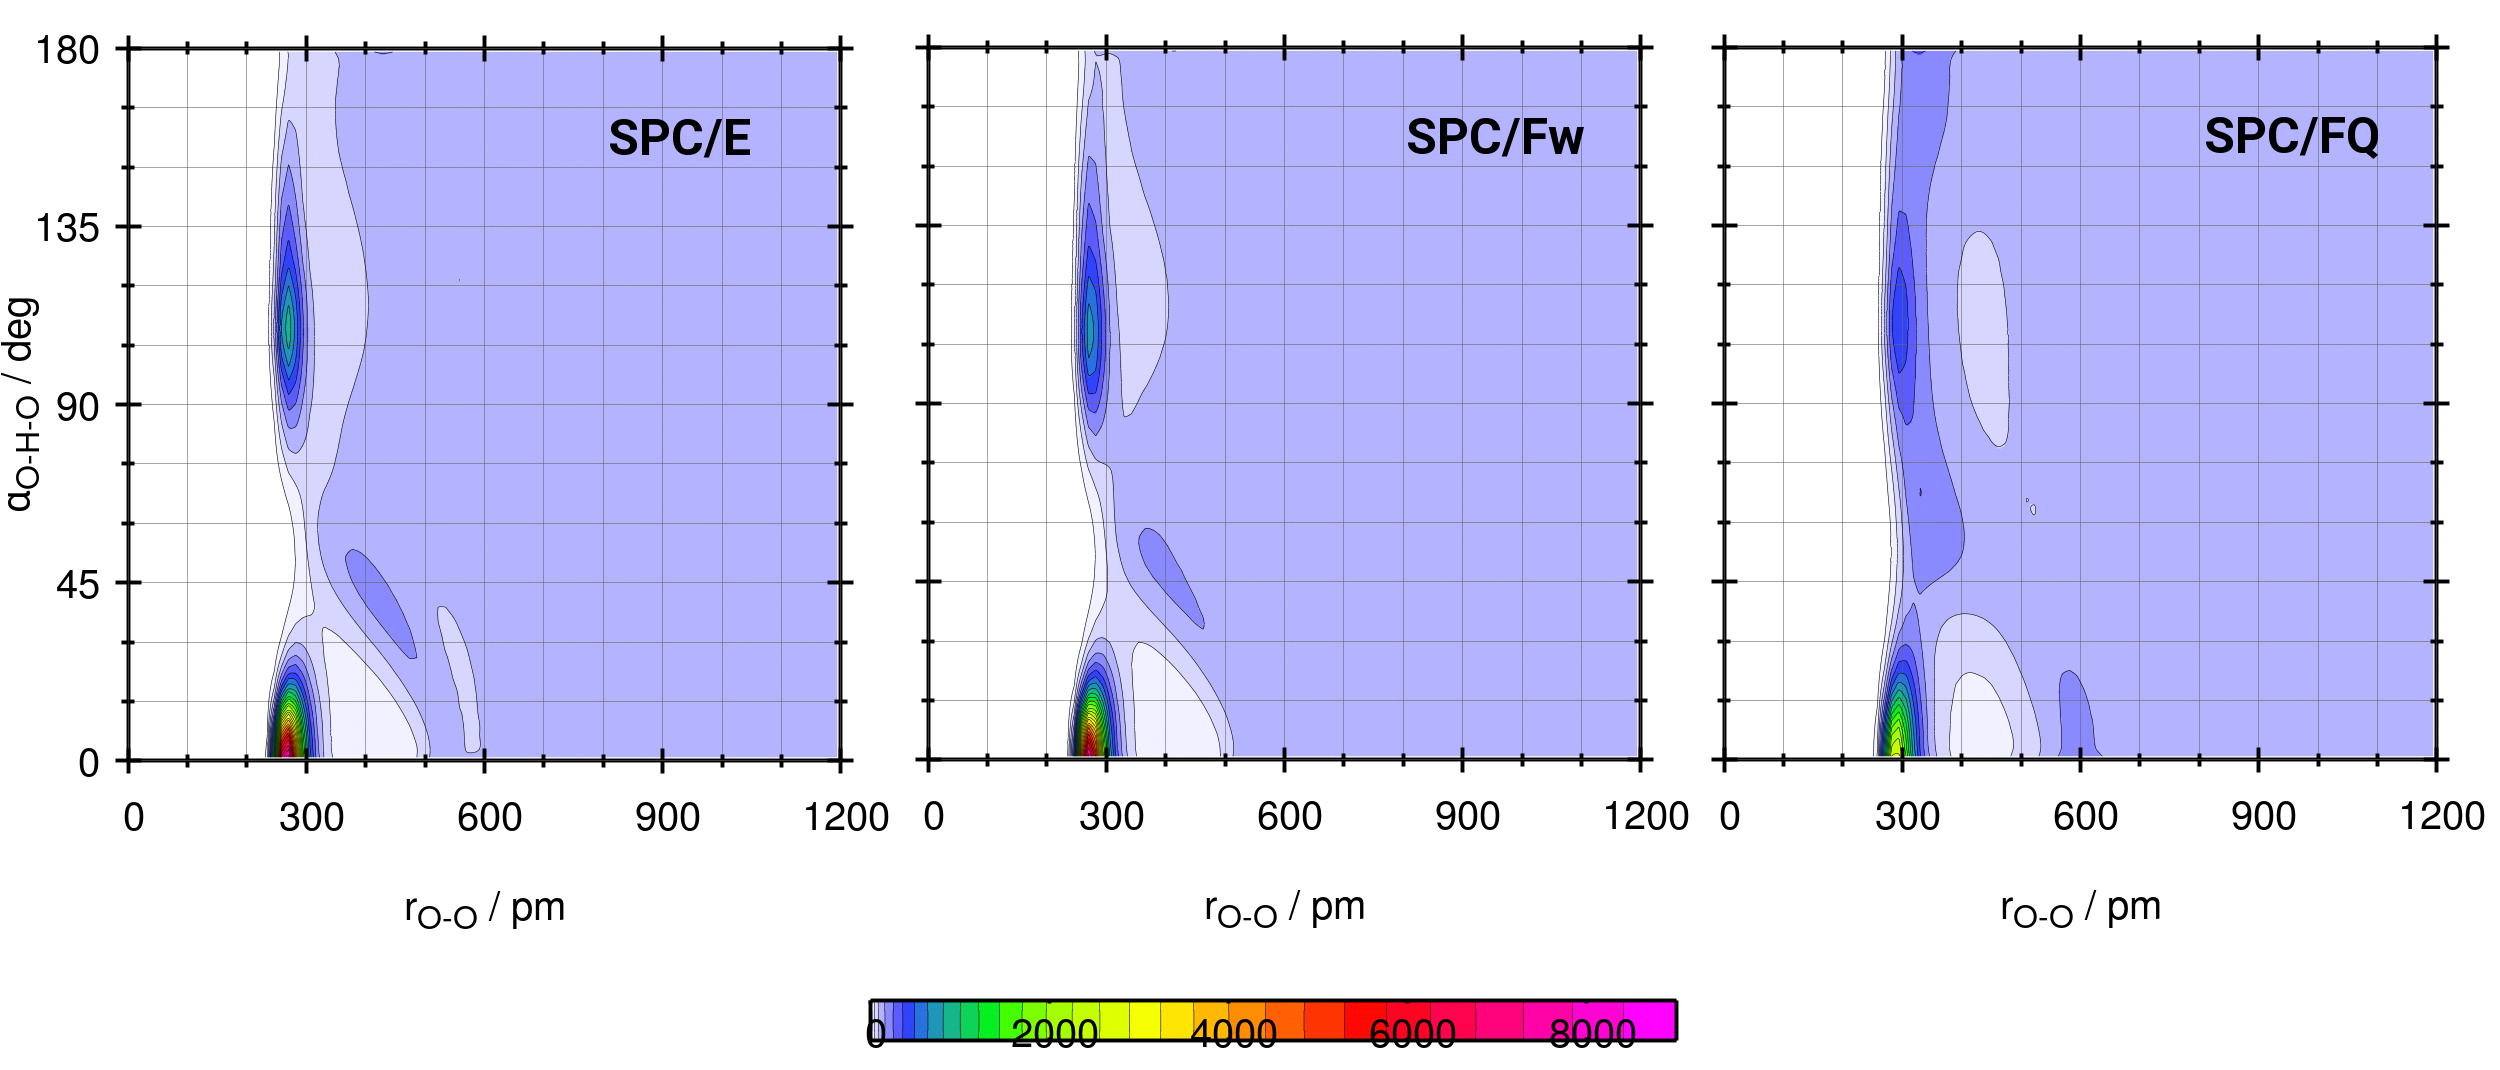
\includegraphics[width=0.95\textwidth]{cdf}
			\caption{Combined radial and angular distribution functions.}
			\label{fig:cdf}
		\end{figure}
	%
	\subsection{Hydrogen Bond Dynamics}
	\label{sec:aggr}
	%
		So far, only structural properties of the systems have been discussed. By performing MD simulations, dynamical properties can be investigated as well. As mentioned before, hydrogen bonds are of great interest in liquid water. Therefore it is reasonable to analyze hydrogen bond dynamics which are described by the life times of these hydrogen bonds. 
		
		To obtain life times from a simulation the dimer autocorrelation function (ACF) of pairs of two water molecules is computed. It is important to precisely define geometrical criteria for water dimers to make sure that the observed property really corresponds to a hydrogen bond lifetime. Previously it was discussed why the angular criterion is chosen as $ 0 \leq \alpha \leq \SI{30}{\degree} $. Furthermore, a distance criterion has to be defined. This is usually chosen as the distance $ r $ at the first minimum in the O--O RDFs. In the present cases, these are $ \SI{326}{\pico\meter}, \SI{330}{\pico\meter}, \SI{450}{\pico\meter}$ for SPC/E, SPC/Fw and SPC/FQ, respectively.
		
		In \autoref{fig:aggr} two kinds of ACFs are depicted, namely the continuous and intermittent ACFs. The former ones count a hydrogen bond as broken forever once the geometrical criteria are not fulfilled. If the hydrogen bond reforms it is counted as a new one. Opposed to that, the latter ones allow for reformation of a hydrogen bond and count it as if it never broke once the criteria are fulfilled again. From these definitions one can figure out that the continuous ACFs will decay faster as compared to the intermittent ones.
		
		In the present case, the ACFs decay in the order SPC/FQ > SPC/Fw > SPC/E for both kinds of ACFs. Taking a closer look at the continuous functions one can find that SPC/E and SPC/Fw behave somewhat similar and the curves are close to each other, whereas the SPC/FQ curve decays way faster. Recapitulating that the SPC/E and SPC/Fw models differ by the presence / absence of flexibility regarding bond stretching and angle bending, it seems questionable weather vibrations have to be included in a water model to describe hydrogen bonds accurately. The SPC/FQ model is more repulsive compared to sPC/E and SPC/Fw as discussed before and yields weaker hydrogen bonds as the curves decay the fastest.
		
		By integrating the ACF, one can obtain the hydrogen bond life time $ \tau $ (see \autoref{tab:tau}). The values clearly display the trend discussed before. Concerning the \enquote{true} values of $ \tau $ it can be said that these should lay in between $ \tau_c $ and $ \tau_i  $.
		%
		\begin{figure}
			\centering
			%% Creator: Matplotlib, PGF backend
%%
%% To include the figure in your LaTeX document, write
%%   \input{<filename>.pgf}
%%
%% Make sure the required packages are loaded in your preamble
%%   \usepackage{pgf}
%%
%% Figures using additional raster images can only be included by \input if
%% they are in the same directory as the main LaTeX file. For loading figures
%% from other directories you can use the `import` package
%%   \usepackage{import}
%% and then include the figures with
%%   \import{<path to file>}{<filename>.pgf}
%%
%% Matplotlib used the following preamble
%%   \usepackage{amssymb} \usepackage{amsmath}
%%
\begingroup%
\makeatletter%
\begin{pgfpicture}%
\pgfpathrectangle{\pgfpointorigin}{\pgfqpoint{6.694230in}{4.016538in}}%
\pgfusepath{use as bounding box, clip}%
\begin{pgfscope}%
\pgfsetbuttcap%
\pgfsetmiterjoin%
\definecolor{currentfill}{rgb}{1.000000,1.000000,1.000000}%
\pgfsetfillcolor{currentfill}%
\pgfsetlinewidth{0.000000pt}%
\definecolor{currentstroke}{rgb}{1.000000,1.000000,1.000000}%
\pgfsetstrokecolor{currentstroke}%
\pgfsetdash{}{0pt}%
\pgfpathmoveto{\pgfqpoint{0.000000in}{0.000000in}}%
\pgfpathlineto{\pgfqpoint{6.694230in}{0.000000in}}%
\pgfpathlineto{\pgfqpoint{6.694230in}{4.016538in}}%
\pgfpathlineto{\pgfqpoint{0.000000in}{4.016538in}}%
\pgfpathclose%
\pgfusepath{fill}%
\end{pgfscope}%
\begin{pgfscope}%
\pgfsetbuttcap%
\pgfsetmiterjoin%
\definecolor{currentfill}{rgb}{1.000000,1.000000,1.000000}%
\pgfsetfillcolor{currentfill}%
\pgfsetlinewidth{0.000000pt}%
\definecolor{currentstroke}{rgb}{0.000000,0.000000,0.000000}%
\pgfsetstrokecolor{currentstroke}%
\pgfsetstrokeopacity{0.000000}%
\pgfsetdash{}{0pt}%
\pgfpathmoveto{\pgfqpoint{0.592518in}{0.525000in}}%
\pgfpathlineto{\pgfqpoint{3.210344in}{0.525000in}}%
\pgfpathlineto{\pgfqpoint{3.210344in}{3.831538in}}%
\pgfpathlineto{\pgfqpoint{0.592518in}{3.831538in}}%
\pgfpathclose%
\pgfusepath{fill}%
\end{pgfscope}%
\begin{pgfscope}%
\pgfsetbuttcap%
\pgfsetroundjoin%
\definecolor{currentfill}{rgb}{0.000000,0.000000,0.000000}%
\pgfsetfillcolor{currentfill}%
\pgfsetlinewidth{0.803000pt}%
\definecolor{currentstroke}{rgb}{0.000000,0.000000,0.000000}%
\pgfsetstrokecolor{currentstroke}%
\pgfsetdash{}{0pt}%
\pgfsys@defobject{currentmarker}{\pgfqpoint{0.000000in}{-0.048611in}}{\pgfqpoint{0.000000in}{0.000000in}}{%
\pgfpathmoveto{\pgfqpoint{0.000000in}{0.000000in}}%
\pgfpathlineto{\pgfqpoint{0.000000in}{-0.048611in}}%
\pgfusepath{stroke,fill}%
}%
\begin{pgfscope}%
\pgfsys@transformshift{0.614153in}{0.525000in}%
\pgfsys@useobject{currentmarker}{}%
\end{pgfscope}%
\end{pgfscope}%
\begin{pgfscope}%
\pgftext[x=0.614153in,y=0.427778in,,top]{\rmfamily\fontsize{8.000000}{9.600000}\selectfont \(\displaystyle 0\)}%
\end{pgfscope}%
\begin{pgfscope}%
\pgfsetbuttcap%
\pgfsetroundjoin%
\definecolor{currentfill}{rgb}{0.000000,0.000000,0.000000}%
\pgfsetfillcolor{currentfill}%
\pgfsetlinewidth{0.803000pt}%
\definecolor{currentstroke}{rgb}{0.000000,0.000000,0.000000}%
\pgfsetstrokecolor{currentstroke}%
\pgfsetdash{}{0pt}%
\pgfsys@defobject{currentmarker}{\pgfqpoint{0.000000in}{-0.048611in}}{\pgfqpoint{0.000000in}{0.000000in}}{%
\pgfpathmoveto{\pgfqpoint{0.000000in}{0.000000in}}%
\pgfpathlineto{\pgfqpoint{0.000000in}{-0.048611in}}%
\pgfusepath{stroke,fill}%
}%
\begin{pgfscope}%
\pgfsys@transformshift{1.046851in}{0.525000in}%
\pgfsys@useobject{currentmarker}{}%
\end{pgfscope}%
\end{pgfscope}%
\begin{pgfscope}%
\pgftext[x=1.046851in,y=0.427778in,,top]{\rmfamily\fontsize{8.000000}{9.600000}\selectfont \(\displaystyle 1\)}%
\end{pgfscope}%
\begin{pgfscope}%
\pgfsetbuttcap%
\pgfsetroundjoin%
\definecolor{currentfill}{rgb}{0.000000,0.000000,0.000000}%
\pgfsetfillcolor{currentfill}%
\pgfsetlinewidth{0.803000pt}%
\definecolor{currentstroke}{rgb}{0.000000,0.000000,0.000000}%
\pgfsetstrokecolor{currentstroke}%
\pgfsetdash{}{0pt}%
\pgfsys@defobject{currentmarker}{\pgfqpoint{0.000000in}{-0.048611in}}{\pgfqpoint{0.000000in}{0.000000in}}{%
\pgfpathmoveto{\pgfqpoint{0.000000in}{0.000000in}}%
\pgfpathlineto{\pgfqpoint{0.000000in}{-0.048611in}}%
\pgfusepath{stroke,fill}%
}%
\begin{pgfscope}%
\pgfsys@transformshift{1.479550in}{0.525000in}%
\pgfsys@useobject{currentmarker}{}%
\end{pgfscope}%
\end{pgfscope}%
\begin{pgfscope}%
\pgftext[x=1.479550in,y=0.427778in,,top]{\rmfamily\fontsize{8.000000}{9.600000}\selectfont \(\displaystyle 2\)}%
\end{pgfscope}%
\begin{pgfscope}%
\pgfsetbuttcap%
\pgfsetroundjoin%
\definecolor{currentfill}{rgb}{0.000000,0.000000,0.000000}%
\pgfsetfillcolor{currentfill}%
\pgfsetlinewidth{0.803000pt}%
\definecolor{currentstroke}{rgb}{0.000000,0.000000,0.000000}%
\pgfsetstrokecolor{currentstroke}%
\pgfsetdash{}{0pt}%
\pgfsys@defobject{currentmarker}{\pgfqpoint{0.000000in}{-0.048611in}}{\pgfqpoint{0.000000in}{0.000000in}}{%
\pgfpathmoveto{\pgfqpoint{0.000000in}{0.000000in}}%
\pgfpathlineto{\pgfqpoint{0.000000in}{-0.048611in}}%
\pgfusepath{stroke,fill}%
}%
\begin{pgfscope}%
\pgfsys@transformshift{1.912248in}{0.525000in}%
\pgfsys@useobject{currentmarker}{}%
\end{pgfscope}%
\end{pgfscope}%
\begin{pgfscope}%
\pgftext[x=1.912248in,y=0.427778in,,top]{\rmfamily\fontsize{8.000000}{9.600000}\selectfont \(\displaystyle 3\)}%
\end{pgfscope}%
\begin{pgfscope}%
\pgfsetbuttcap%
\pgfsetroundjoin%
\definecolor{currentfill}{rgb}{0.000000,0.000000,0.000000}%
\pgfsetfillcolor{currentfill}%
\pgfsetlinewidth{0.803000pt}%
\definecolor{currentstroke}{rgb}{0.000000,0.000000,0.000000}%
\pgfsetstrokecolor{currentstroke}%
\pgfsetdash{}{0pt}%
\pgfsys@defobject{currentmarker}{\pgfqpoint{0.000000in}{-0.048611in}}{\pgfqpoint{0.000000in}{0.000000in}}{%
\pgfpathmoveto{\pgfqpoint{0.000000in}{0.000000in}}%
\pgfpathlineto{\pgfqpoint{0.000000in}{-0.048611in}}%
\pgfusepath{stroke,fill}%
}%
\begin{pgfscope}%
\pgfsys@transformshift{2.344947in}{0.525000in}%
\pgfsys@useobject{currentmarker}{}%
\end{pgfscope}%
\end{pgfscope}%
\begin{pgfscope}%
\pgftext[x=2.344947in,y=0.427778in,,top]{\rmfamily\fontsize{8.000000}{9.600000}\selectfont \(\displaystyle 4\)}%
\end{pgfscope}%
\begin{pgfscope}%
\pgfsetbuttcap%
\pgfsetroundjoin%
\definecolor{currentfill}{rgb}{0.000000,0.000000,0.000000}%
\pgfsetfillcolor{currentfill}%
\pgfsetlinewidth{0.803000pt}%
\definecolor{currentstroke}{rgb}{0.000000,0.000000,0.000000}%
\pgfsetstrokecolor{currentstroke}%
\pgfsetdash{}{0pt}%
\pgfsys@defobject{currentmarker}{\pgfqpoint{0.000000in}{-0.048611in}}{\pgfqpoint{0.000000in}{0.000000in}}{%
\pgfpathmoveto{\pgfqpoint{0.000000in}{0.000000in}}%
\pgfpathlineto{\pgfqpoint{0.000000in}{-0.048611in}}%
\pgfusepath{stroke,fill}%
}%
\begin{pgfscope}%
\pgfsys@transformshift{2.777645in}{0.525000in}%
\pgfsys@useobject{currentmarker}{}%
\end{pgfscope}%
\end{pgfscope}%
\begin{pgfscope}%
\pgftext[x=2.777645in,y=0.427778in,,top]{\rmfamily\fontsize{8.000000}{9.600000}\selectfont \(\displaystyle 5\)}%
\end{pgfscope}%
\begin{pgfscope}%
\pgfsetbuttcap%
\pgfsetroundjoin%
\definecolor{currentfill}{rgb}{0.000000,0.000000,0.000000}%
\pgfsetfillcolor{currentfill}%
\pgfsetlinewidth{0.803000pt}%
\definecolor{currentstroke}{rgb}{0.000000,0.000000,0.000000}%
\pgfsetstrokecolor{currentstroke}%
\pgfsetdash{}{0pt}%
\pgfsys@defobject{currentmarker}{\pgfqpoint{0.000000in}{-0.048611in}}{\pgfqpoint{0.000000in}{0.000000in}}{%
\pgfpathmoveto{\pgfqpoint{0.000000in}{0.000000in}}%
\pgfpathlineto{\pgfqpoint{0.000000in}{-0.048611in}}%
\pgfusepath{stroke,fill}%
}%
\begin{pgfscope}%
\pgfsys@transformshift{3.210344in}{0.525000in}%
\pgfsys@useobject{currentmarker}{}%
\end{pgfscope}%
\end{pgfscope}%
\begin{pgfscope}%
\pgftext[x=3.210344in,y=0.427778in,,top]{\rmfamily\fontsize{8.000000}{9.600000}\selectfont \(\displaystyle 6\)}%
\end{pgfscope}%
\begin{pgfscope}%
\pgftext[x=1.901431in,y=0.273457in,,top]{\rmfamily\fontsize{10.000000}{12.000000}\selectfont \(\displaystyle \tau\) in ps}%
\end{pgfscope}%
\begin{pgfscope}%
\pgfsetbuttcap%
\pgfsetroundjoin%
\definecolor{currentfill}{rgb}{0.000000,0.000000,0.000000}%
\pgfsetfillcolor{currentfill}%
\pgfsetlinewidth{0.803000pt}%
\definecolor{currentstroke}{rgb}{0.000000,0.000000,0.000000}%
\pgfsetstrokecolor{currentstroke}%
\pgfsetdash{}{0pt}%
\pgfsys@defobject{currentmarker}{\pgfqpoint{-0.048611in}{0.000000in}}{\pgfqpoint{0.000000in}{0.000000in}}{%
\pgfpathmoveto{\pgfqpoint{0.000000in}{0.000000in}}%
\pgfpathlineto{\pgfqpoint{-0.048611in}{0.000000in}}%
\pgfusepath{stroke,fill}%
}%
\begin{pgfscope}%
\pgfsys@transformshift{0.592518in}{0.557417in}%
\pgfsys@useobject{currentmarker}{}%
\end{pgfscope}%
\end{pgfscope}%
\begin{pgfscope}%
\pgftext[x=0.344444in,y=0.518837in,left,base]{\rmfamily\fontsize{8.000000}{9.600000}\selectfont \(\displaystyle 0.0\)}%
\end{pgfscope}%
\begin{pgfscope}%
\pgfsetbuttcap%
\pgfsetroundjoin%
\definecolor{currentfill}{rgb}{0.000000,0.000000,0.000000}%
\pgfsetfillcolor{currentfill}%
\pgfsetlinewidth{0.803000pt}%
\definecolor{currentstroke}{rgb}{0.000000,0.000000,0.000000}%
\pgfsetstrokecolor{currentstroke}%
\pgfsetdash{}{0pt}%
\pgfsys@defobject{currentmarker}{\pgfqpoint{-0.048611in}{0.000000in}}{\pgfqpoint{0.000000in}{0.000000in}}{%
\pgfpathmoveto{\pgfqpoint{0.000000in}{0.000000in}}%
\pgfpathlineto{\pgfqpoint{-0.048611in}{0.000000in}}%
\pgfusepath{stroke,fill}%
}%
\begin{pgfscope}%
\pgfsys@transformshift{0.592518in}{1.205758in}%
\pgfsys@useobject{currentmarker}{}%
\end{pgfscope}%
\end{pgfscope}%
\begin{pgfscope}%
\pgftext[x=0.344444in,y=1.167178in,left,base]{\rmfamily\fontsize{8.000000}{9.600000}\selectfont \(\displaystyle 0.2\)}%
\end{pgfscope}%
\begin{pgfscope}%
\pgfsetbuttcap%
\pgfsetroundjoin%
\definecolor{currentfill}{rgb}{0.000000,0.000000,0.000000}%
\pgfsetfillcolor{currentfill}%
\pgfsetlinewidth{0.803000pt}%
\definecolor{currentstroke}{rgb}{0.000000,0.000000,0.000000}%
\pgfsetstrokecolor{currentstroke}%
\pgfsetdash{}{0pt}%
\pgfsys@defobject{currentmarker}{\pgfqpoint{-0.048611in}{0.000000in}}{\pgfqpoint{0.000000in}{0.000000in}}{%
\pgfpathmoveto{\pgfqpoint{0.000000in}{0.000000in}}%
\pgfpathlineto{\pgfqpoint{-0.048611in}{0.000000in}}%
\pgfusepath{stroke,fill}%
}%
\begin{pgfscope}%
\pgfsys@transformshift{0.592518in}{1.854099in}%
\pgfsys@useobject{currentmarker}{}%
\end{pgfscope}%
\end{pgfscope}%
\begin{pgfscope}%
\pgftext[x=0.344444in,y=1.815518in,left,base]{\rmfamily\fontsize{8.000000}{9.600000}\selectfont \(\displaystyle 0.4\)}%
\end{pgfscope}%
\begin{pgfscope}%
\pgfsetbuttcap%
\pgfsetroundjoin%
\definecolor{currentfill}{rgb}{0.000000,0.000000,0.000000}%
\pgfsetfillcolor{currentfill}%
\pgfsetlinewidth{0.803000pt}%
\definecolor{currentstroke}{rgb}{0.000000,0.000000,0.000000}%
\pgfsetstrokecolor{currentstroke}%
\pgfsetdash{}{0pt}%
\pgfsys@defobject{currentmarker}{\pgfqpoint{-0.048611in}{0.000000in}}{\pgfqpoint{0.000000in}{0.000000in}}{%
\pgfpathmoveto{\pgfqpoint{0.000000in}{0.000000in}}%
\pgfpathlineto{\pgfqpoint{-0.048611in}{0.000000in}}%
\pgfusepath{stroke,fill}%
}%
\begin{pgfscope}%
\pgfsys@transformshift{0.592518in}{2.502439in}%
\pgfsys@useobject{currentmarker}{}%
\end{pgfscope}%
\end{pgfscope}%
\begin{pgfscope}%
\pgftext[x=0.344444in,y=2.463859in,left,base]{\rmfamily\fontsize{8.000000}{9.600000}\selectfont \(\displaystyle 0.6\)}%
\end{pgfscope}%
\begin{pgfscope}%
\pgfsetbuttcap%
\pgfsetroundjoin%
\definecolor{currentfill}{rgb}{0.000000,0.000000,0.000000}%
\pgfsetfillcolor{currentfill}%
\pgfsetlinewidth{0.803000pt}%
\definecolor{currentstroke}{rgb}{0.000000,0.000000,0.000000}%
\pgfsetstrokecolor{currentstroke}%
\pgfsetdash{}{0pt}%
\pgfsys@defobject{currentmarker}{\pgfqpoint{-0.048611in}{0.000000in}}{\pgfqpoint{0.000000in}{0.000000in}}{%
\pgfpathmoveto{\pgfqpoint{0.000000in}{0.000000in}}%
\pgfpathlineto{\pgfqpoint{-0.048611in}{0.000000in}}%
\pgfusepath{stroke,fill}%
}%
\begin{pgfscope}%
\pgfsys@transformshift{0.592518in}{3.150780in}%
\pgfsys@useobject{currentmarker}{}%
\end{pgfscope}%
\end{pgfscope}%
\begin{pgfscope}%
\pgftext[x=0.344444in,y=3.112200in,left,base]{\rmfamily\fontsize{8.000000}{9.600000}\selectfont \(\displaystyle 0.8\)}%
\end{pgfscope}%
\begin{pgfscope}%
\pgfsetbuttcap%
\pgfsetroundjoin%
\definecolor{currentfill}{rgb}{0.000000,0.000000,0.000000}%
\pgfsetfillcolor{currentfill}%
\pgfsetlinewidth{0.803000pt}%
\definecolor{currentstroke}{rgb}{0.000000,0.000000,0.000000}%
\pgfsetstrokecolor{currentstroke}%
\pgfsetdash{}{0pt}%
\pgfsys@defobject{currentmarker}{\pgfqpoint{-0.048611in}{0.000000in}}{\pgfqpoint{0.000000in}{0.000000in}}{%
\pgfpathmoveto{\pgfqpoint{0.000000in}{0.000000in}}%
\pgfpathlineto{\pgfqpoint{-0.048611in}{0.000000in}}%
\pgfusepath{stroke,fill}%
}%
\begin{pgfscope}%
\pgfsys@transformshift{0.592518in}{3.799121in}%
\pgfsys@useobject{currentmarker}{}%
\end{pgfscope}%
\end{pgfscope}%
\begin{pgfscope}%
\pgftext[x=0.344444in,y=3.760541in,left,base]{\rmfamily\fontsize{8.000000}{9.600000}\selectfont \(\displaystyle 1.0\)}%
\end{pgfscope}%
\begin{pgfscope}%
\pgftext[x=0.288889in,y=2.178269in,,bottom,rotate=90.000000]{\rmfamily\fontsize{10.000000}{12.000000}\selectfont \(\displaystyle A(\tau)\)}%
\end{pgfscope}%
\begin{pgfscope}%
\pgfpathrectangle{\pgfqpoint{0.592518in}{0.525000in}}{\pgfqpoint{2.617826in}{3.306538in}} %
\pgfusepath{clip}%
\pgfsetrectcap%
\pgfsetroundjoin%
\pgfsetlinewidth{1.003750pt}%
\definecolor{currentstroke}{rgb}{0.000000,0.000000,0.000000}%
\pgfsetstrokecolor{currentstroke}%
\pgfsetdash{}{0pt}%
\pgfpathmoveto{\pgfqpoint{0.614153in}{3.799121in}}%
\pgfpathlineto{\pgfqpoint{0.624970in}{3.618301in}}%
\pgfpathlineto{\pgfqpoint{0.635787in}{3.473274in}}%
\pgfpathlineto{\pgfqpoint{0.646605in}{3.356440in}}%
\pgfpathlineto{\pgfqpoint{0.666076in}{3.173337in}}%
\pgfpathlineto{\pgfqpoint{0.683384in}{3.030209in}}%
\pgfpathlineto{\pgfqpoint{0.705019in}{2.871035in}}%
\pgfpathlineto{\pgfqpoint{0.728818in}{2.714041in}}%
\pgfpathlineto{\pgfqpoint{0.752616in}{2.572284in}}%
\pgfpathlineto{\pgfqpoint{0.776414in}{2.443534in}}%
\pgfpathlineto{\pgfqpoint{0.800213in}{2.326058in}}%
\pgfpathlineto{\pgfqpoint{0.826175in}{2.209134in}}%
\pgfpathlineto{\pgfqpoint{0.852137in}{2.102425in}}%
\pgfpathlineto{\pgfqpoint{0.878099in}{2.004575in}}%
\pgfpathlineto{\pgfqpoint{0.906224in}{1.907316in}}%
\pgfpathlineto{\pgfqpoint{0.934349in}{1.818070in}}%
\pgfpathlineto{\pgfqpoint{0.962475in}{1.735952in}}%
\pgfpathlineto{\pgfqpoint{0.990600in}{1.660220in}}%
\pgfpathlineto{\pgfqpoint{1.020889in}{1.585070in}}%
\pgfpathlineto{\pgfqpoint{1.051178in}{1.515849in}}%
\pgfpathlineto{\pgfqpoint{1.081467in}{1.451940in}}%
\pgfpathlineto{\pgfqpoint{1.113919in}{1.388828in}}%
\pgfpathlineto{\pgfqpoint{1.146372in}{1.330722in}}%
\pgfpathlineto{\pgfqpoint{1.178824in}{1.277174in}}%
\pgfpathlineto{\pgfqpoint{1.211276in}{1.227765in}}%
\pgfpathlineto{\pgfqpoint{1.245892in}{1.179166in}}%
\pgfpathlineto{\pgfqpoint{1.280508in}{1.134437in}}%
\pgfpathlineto{\pgfqpoint{1.315124in}{1.093252in}}%
\pgfpathlineto{\pgfqpoint{1.351903in}{1.052953in}}%
\pgfpathlineto{\pgfqpoint{1.388683in}{1.015888in}}%
\pgfpathlineto{\pgfqpoint{1.425462in}{0.981843in}}%
\pgfpathlineto{\pgfqpoint{1.464405in}{0.948717in}}%
\pgfpathlineto{\pgfqpoint{1.505511in}{0.916731in}}%
\pgfpathlineto{\pgfqpoint{1.546618in}{0.887527in}}%
\pgfpathlineto{\pgfqpoint{1.589888in}{0.859494in}}%
\pgfpathlineto{\pgfqpoint{1.635321in}{0.832744in}}%
\pgfpathlineto{\pgfqpoint{1.682918in}{0.807407in}}%
\pgfpathlineto{\pgfqpoint{1.732678in}{0.783539in}}%
\pgfpathlineto{\pgfqpoint{1.784602in}{0.761154in}}%
\pgfpathlineto{\pgfqpoint{1.838689in}{0.740305in}}%
\pgfpathlineto{\pgfqpoint{1.897104in}{0.720299in}}%
\pgfpathlineto{\pgfqpoint{1.957681in}{0.701919in}}%
\pgfpathlineto{\pgfqpoint{2.022586in}{0.684589in}}%
\pgfpathlineto{\pgfqpoint{2.091818in}{0.668463in}}%
\pgfpathlineto{\pgfqpoint{2.165377in}{0.653642in}}%
\pgfpathlineto{\pgfqpoint{2.245426in}{0.639822in}}%
\pgfpathlineto{\pgfqpoint{2.331966in}{0.627124in}}%
\pgfpathlineto{\pgfqpoint{2.429323in}{0.615181in}}%
\pgfpathlineto{\pgfqpoint{2.533170in}{0.604748in}}%
\pgfpathlineto{\pgfqpoint{2.649999in}{0.595272in}}%
\pgfpathlineto{\pgfqpoint{2.784136in}{0.586758in}}%
\pgfpathlineto{\pgfqpoint{2.937743in}{0.579332in}}%
\pgfpathlineto{\pgfqpoint{3.110823in}{0.573208in}}%
\pgfpathlineto{\pgfqpoint{3.212507in}{0.570451in}}%
\pgfpathlineto{\pgfqpoint{3.212507in}{0.570451in}}%
\pgfusepath{stroke}%
\end{pgfscope}%
\begin{pgfscope}%
\pgfpathrectangle{\pgfqpoint{0.592518in}{0.525000in}}{\pgfqpoint{2.617826in}{3.306538in}} %
\pgfusepath{clip}%
\pgfsetbuttcap%
\pgfsetroundjoin%
\pgfsetlinewidth{0.301125pt}%
\definecolor{currentstroke}{rgb}{0.000000,0.000000,0.000000}%
\pgfsetstrokecolor{currentstroke}%
\pgfsetdash{{1.110000pt}{0.480000pt}}{0.000000pt}%
\pgfpathmoveto{\pgfqpoint{0.592518in}{0.557417in}}%
\pgfpathlineto{\pgfqpoint{3.210344in}{0.557417in}}%
\pgfusepath{stroke}%
\end{pgfscope}%
\begin{pgfscope}%
\pgfpathrectangle{\pgfqpoint{0.592518in}{0.525000in}}{\pgfqpoint{2.617826in}{3.306538in}} %
\pgfusepath{clip}%
\pgfsetrectcap%
\pgfsetroundjoin%
\pgfsetlinewidth{1.003750pt}%
\definecolor{currentstroke}{rgb}{1.000000,0.000000,0.000000}%
\pgfsetstrokecolor{currentstroke}%
\pgfsetdash{}{0pt}%
\pgfpathmoveto{\pgfqpoint{0.614153in}{3.799121in}}%
\pgfpathlineto{\pgfqpoint{0.622807in}{3.602079in}}%
\pgfpathlineto{\pgfqpoint{0.633624in}{3.406765in}}%
\pgfpathlineto{\pgfqpoint{0.644441in}{3.252576in}}%
\pgfpathlineto{\pgfqpoint{0.659586in}{3.072393in}}%
\pgfpathlineto{\pgfqpoint{0.676894in}{2.891612in}}%
\pgfpathlineto{\pgfqpoint{0.694202in}{2.734167in}}%
\pgfpathlineto{\pgfqpoint{0.713673in}{2.576613in}}%
\pgfpathlineto{\pgfqpoint{0.735308in}{2.419999in}}%
\pgfpathlineto{\pgfqpoint{0.756943in}{2.279338in}}%
\pgfpathlineto{\pgfqpoint{0.778578in}{2.152214in}}%
\pgfpathlineto{\pgfqpoint{0.802376in}{2.025860in}}%
\pgfpathlineto{\pgfqpoint{0.826175in}{1.911834in}}%
\pgfpathlineto{\pgfqpoint{0.849973in}{1.808517in}}%
\pgfpathlineto{\pgfqpoint{0.873772in}{1.714601in}}%
\pgfpathlineto{\pgfqpoint{0.899734in}{1.621481in}}%
\pgfpathlineto{\pgfqpoint{0.925695in}{1.536924in}}%
\pgfpathlineto{\pgfqpoint{0.951657in}{1.459947in}}%
\pgfpathlineto{\pgfqpoint{0.977619in}{1.389751in}}%
\pgfpathlineto{\pgfqpoint{1.003581in}{1.325626in}}%
\pgfpathlineto{\pgfqpoint{1.031707in}{1.262229in}}%
\pgfpathlineto{\pgfqpoint{1.059832in}{1.204526in}}%
\pgfpathlineto{\pgfqpoint{1.087957in}{1.151943in}}%
\pgfpathlineto{\pgfqpoint{1.116083in}{1.103943in}}%
\pgfpathlineto{\pgfqpoint{1.144208in}{1.060080in}}%
\pgfpathlineto{\pgfqpoint{1.174497in}{1.017025in}}%
\pgfpathlineto{\pgfqpoint{1.204786in}{0.977898in}}%
\pgfpathlineto{\pgfqpoint{1.235075in}{0.942274in}}%
\pgfpathlineto{\pgfqpoint{1.267527in}{0.907576in}}%
\pgfpathlineto{\pgfqpoint{1.299980in}{0.876137in}}%
\pgfpathlineto{\pgfqpoint{1.334596in}{0.845815in}}%
\pgfpathlineto{\pgfqpoint{1.369211in}{0.818479in}}%
\pgfpathlineto{\pgfqpoint{1.405991in}{0.792387in}}%
\pgfpathlineto{\pgfqpoint{1.442770in}{0.769006in}}%
\pgfpathlineto{\pgfqpoint{1.481713in}{0.746853in}}%
\pgfpathlineto{\pgfqpoint{1.522819in}{0.726089in}}%
\pgfpathlineto{\pgfqpoint{1.566089in}{0.706762in}}%
\pgfpathlineto{\pgfqpoint{1.611523in}{0.688887in}}%
\pgfpathlineto{\pgfqpoint{1.659119in}{0.672489in}}%
\pgfpathlineto{\pgfqpoint{1.711043in}{0.656911in}}%
\pgfpathlineto{\pgfqpoint{1.765131in}{0.642943in}}%
\pgfpathlineto{\pgfqpoint{1.825708in}{0.629644in}}%
\pgfpathlineto{\pgfqpoint{1.890613in}{0.617735in}}%
\pgfpathlineto{\pgfqpoint{1.962008in}{0.606948in}}%
\pgfpathlineto{\pgfqpoint{2.042058in}{0.597176in}}%
\pgfpathlineto{\pgfqpoint{2.130761in}{0.588645in}}%
\pgfpathlineto{\pgfqpoint{2.234608in}{0.581017in}}%
\pgfpathlineto{\pgfqpoint{2.353601in}{0.574569in}}%
\pgfpathlineto{\pgfqpoint{2.496391in}{0.569154in}}%
\pgfpathlineto{\pgfqpoint{2.675961in}{0.564697in}}%
\pgfpathlineto{\pgfqpoint{2.905291in}{0.561361in}}%
\pgfpathlineto{\pgfqpoint{3.212507in}{0.559159in}}%
\pgfpathlineto{\pgfqpoint{3.212507in}{0.559159in}}%
\pgfusepath{stroke}%
\end{pgfscope}%
\begin{pgfscope}%
\pgfpathrectangle{\pgfqpoint{0.592518in}{0.525000in}}{\pgfqpoint{2.617826in}{3.306538in}} %
\pgfusepath{clip}%
\pgfsetbuttcap%
\pgfsetroundjoin%
\pgfsetlinewidth{0.301125pt}%
\definecolor{currentstroke}{rgb}{0.000000,0.000000,0.000000}%
\pgfsetstrokecolor{currentstroke}%
\pgfsetdash{{1.110000pt}{0.480000pt}}{0.000000pt}%
\pgfpathmoveto{\pgfqpoint{0.592518in}{0.557417in}}%
\pgfpathlineto{\pgfqpoint{3.210344in}{0.557417in}}%
\pgfusepath{stroke}%
\end{pgfscope}%
\begin{pgfscope}%
\pgfpathrectangle{\pgfqpoint{0.592518in}{0.525000in}}{\pgfqpoint{2.617826in}{3.306538in}} %
\pgfusepath{clip}%
\pgfsetrectcap%
\pgfsetroundjoin%
\pgfsetlinewidth{1.003750pt}%
\definecolor{currentstroke}{rgb}{0.000000,0.000000,1.000000}%
\pgfsetstrokecolor{currentstroke}%
\pgfsetdash{}{0pt}%
\pgfpathmoveto{\pgfqpoint{0.614153in}{3.799121in}}%
\pgfpathlineto{\pgfqpoint{0.622807in}{3.081767in}}%
\pgfpathlineto{\pgfqpoint{0.629297in}{2.710736in}}%
\pgfpathlineto{\pgfqpoint{0.635787in}{2.447265in}}%
\pgfpathlineto{\pgfqpoint{0.644441in}{2.191020in}}%
\pgfpathlineto{\pgfqpoint{0.653095in}{1.996975in}}%
\pgfpathlineto{\pgfqpoint{0.663913in}{1.801972in}}%
\pgfpathlineto{\pgfqpoint{0.676894in}{1.611899in}}%
\pgfpathlineto{\pgfqpoint{0.689875in}{1.457546in}}%
\pgfpathlineto{\pgfqpoint{0.702856in}{1.330222in}}%
\pgfpathlineto{\pgfqpoint{0.715837in}{1.223490in}}%
\pgfpathlineto{\pgfqpoint{0.728818in}{1.133029in}}%
\pgfpathlineto{\pgfqpoint{0.741799in}{1.055870in}}%
\pgfpathlineto{\pgfqpoint{0.756943in}{0.979780in}}%
\pgfpathlineto{\pgfqpoint{0.772088in}{0.916060in}}%
\pgfpathlineto{\pgfqpoint{0.787232in}{0.862496in}}%
\pgfpathlineto{\pgfqpoint{0.802376in}{0.817246in}}%
\pgfpathlineto{\pgfqpoint{0.817521in}{0.778972in}}%
\pgfpathlineto{\pgfqpoint{0.832665in}{0.746550in}}%
\pgfpathlineto{\pgfqpoint{0.847810in}{0.719015in}}%
\pgfpathlineto{\pgfqpoint{0.862954in}{0.695586in}}%
\pgfpathlineto{\pgfqpoint{0.880262in}{0.673017in}}%
\pgfpathlineto{\pgfqpoint{0.897570in}{0.654189in}}%
\pgfpathlineto{\pgfqpoint{0.914878in}{0.638467in}}%
\pgfpathlineto{\pgfqpoint{0.934349in}{0.623846in}}%
\pgfpathlineto{\pgfqpoint{0.953821in}{0.611901in}}%
\pgfpathlineto{\pgfqpoint{0.975456in}{0.601140in}}%
\pgfpathlineto{\pgfqpoint{0.999254in}{0.591764in}}%
\pgfpathlineto{\pgfqpoint{1.027380in}{0.583255in}}%
\pgfpathlineto{\pgfqpoint{1.057669in}{0.576456in}}%
\pgfpathlineto{\pgfqpoint{1.094448in}{0.570577in}}%
\pgfpathlineto{\pgfqpoint{1.137718in}{0.565978in}}%
\pgfpathlineto{\pgfqpoint{1.196132in}{0.562181in}}%
\pgfpathlineto{\pgfqpoint{1.274018in}{0.559565in}}%
\pgfpathlineto{\pgfqpoint{1.395173in}{0.558024in}}%
\pgfpathlineto{\pgfqpoint{1.659119in}{0.557461in}}%
\pgfpathlineto{\pgfqpoint{3.212507in}{0.557417in}}%
\pgfpathlineto{\pgfqpoint{3.212507in}{0.557417in}}%
\pgfusepath{stroke}%
\end{pgfscope}%
\begin{pgfscope}%
\pgfpathrectangle{\pgfqpoint{0.592518in}{0.525000in}}{\pgfqpoint{2.617826in}{3.306538in}} %
\pgfusepath{clip}%
\pgfsetbuttcap%
\pgfsetroundjoin%
\pgfsetlinewidth{0.301125pt}%
\definecolor{currentstroke}{rgb}{0.000000,0.000000,0.000000}%
\pgfsetstrokecolor{currentstroke}%
\pgfsetdash{{1.110000pt}{0.480000pt}}{0.000000pt}%
\pgfpathmoveto{\pgfqpoint{0.592518in}{0.557417in}}%
\pgfpathlineto{\pgfqpoint{3.210344in}{0.557417in}}%
\pgfusepath{stroke}%
\end{pgfscope}%
\begin{pgfscope}%
\pgfsetrectcap%
\pgfsetmiterjoin%
\pgfsetlinewidth{0.803000pt}%
\definecolor{currentstroke}{rgb}{0.000000,0.000000,0.000000}%
\pgfsetstrokecolor{currentstroke}%
\pgfsetdash{}{0pt}%
\pgfpathmoveto{\pgfqpoint{0.592518in}{0.525000in}}%
\pgfpathlineto{\pgfqpoint{0.592518in}{3.831538in}}%
\pgfusepath{stroke}%
\end{pgfscope}%
\begin{pgfscope}%
\pgfsetrectcap%
\pgfsetmiterjoin%
\pgfsetlinewidth{0.803000pt}%
\definecolor{currentstroke}{rgb}{0.000000,0.000000,0.000000}%
\pgfsetstrokecolor{currentstroke}%
\pgfsetdash{}{0pt}%
\pgfpathmoveto{\pgfqpoint{3.210344in}{0.525000in}}%
\pgfpathlineto{\pgfqpoint{3.210344in}{3.831538in}}%
\pgfusepath{stroke}%
\end{pgfscope}%
\begin{pgfscope}%
\pgfsetrectcap%
\pgfsetmiterjoin%
\pgfsetlinewidth{0.803000pt}%
\definecolor{currentstroke}{rgb}{0.000000,0.000000,0.000000}%
\pgfsetstrokecolor{currentstroke}%
\pgfsetdash{}{0pt}%
\pgfpathmoveto{\pgfqpoint{0.592518in}{0.525000in}}%
\pgfpathlineto{\pgfqpoint{3.210344in}{0.525000in}}%
\pgfusepath{stroke}%
\end{pgfscope}%
\begin{pgfscope}%
\pgfsetrectcap%
\pgfsetmiterjoin%
\pgfsetlinewidth{0.803000pt}%
\definecolor{currentstroke}{rgb}{0.000000,0.000000,0.000000}%
\pgfsetstrokecolor{currentstroke}%
\pgfsetdash{}{0pt}%
\pgfpathmoveto{\pgfqpoint{0.592518in}{3.831538in}}%
\pgfpathlineto{\pgfqpoint{3.210344in}{3.831538in}}%
\pgfusepath{stroke}%
\end{pgfscope}%
\begin{pgfscope}%
\pgfsetbuttcap%
\pgfsetmiterjoin%
\definecolor{currentfill}{rgb}{1.000000,1.000000,1.000000}%
\pgfsetfillcolor{currentfill}%
\pgfsetfillopacity{0.800000}%
\pgfsetlinewidth{1.003750pt}%
\definecolor{currentstroke}{rgb}{0.800000,0.800000,0.800000}%
\pgfsetstrokecolor{currentstroke}%
\pgfsetstrokeopacity{0.800000}%
\pgfsetdash{}{0pt}%
\pgfpathmoveto{\pgfqpoint{2.324573in}{3.254377in}}%
\pgfpathlineto{\pgfqpoint{3.132566in}{3.254377in}}%
\pgfpathquadraticcurveto{\pgfqpoint{3.154788in}{3.254377in}}{\pgfqpoint{3.154788in}{3.276600in}}%
\pgfpathlineto{\pgfqpoint{3.154788in}{3.753760in}}%
\pgfpathquadraticcurveto{\pgfqpoint{3.154788in}{3.775982in}}{\pgfqpoint{3.132566in}{3.775982in}}%
\pgfpathlineto{\pgfqpoint{2.324573in}{3.775982in}}%
\pgfpathquadraticcurveto{\pgfqpoint{2.302351in}{3.775982in}}{\pgfqpoint{2.302351in}{3.753760in}}%
\pgfpathlineto{\pgfqpoint{2.302351in}{3.276600in}}%
\pgfpathquadraticcurveto{\pgfqpoint{2.302351in}{3.254377in}}{\pgfqpoint{2.324573in}{3.254377in}}%
\pgfpathclose%
\pgfusepath{stroke,fill}%
\end{pgfscope}%
\begin{pgfscope}%
\pgfsetrectcap%
\pgfsetroundjoin%
\pgfsetlinewidth{1.003750pt}%
\definecolor{currentstroke}{rgb}{0.000000,0.000000,0.000000}%
\pgfsetstrokecolor{currentstroke}%
\pgfsetdash{}{0pt}%
\pgfpathmoveto{\pgfqpoint{2.346795in}{3.687094in}}%
\pgfpathlineto{\pgfqpoint{2.569018in}{3.687094in}}%
\pgfusepath{stroke}%
\end{pgfscope}%
\begin{pgfscope}%
\pgftext[x=2.657906in,y=3.648205in,left,base]{\rmfamily\fontsize{8.000000}{9.600000}\selectfont SPC/E}%
\end{pgfscope}%
\begin{pgfscope}%
\pgfsetrectcap%
\pgfsetroundjoin%
\pgfsetlinewidth{1.003750pt}%
\definecolor{currentstroke}{rgb}{1.000000,0.000000,0.000000}%
\pgfsetstrokecolor{currentstroke}%
\pgfsetdash{}{0pt}%
\pgfpathmoveto{\pgfqpoint{2.346795in}{3.520427in}}%
\pgfpathlineto{\pgfqpoint{2.569018in}{3.520427in}}%
\pgfusepath{stroke}%
\end{pgfscope}%
\begin{pgfscope}%
\pgftext[x=2.657906in,y=3.481538in,left,base]{\rmfamily\fontsize{8.000000}{9.600000}\selectfont SPC/Fw}%
\end{pgfscope}%
\begin{pgfscope}%
\pgfsetrectcap%
\pgfsetroundjoin%
\pgfsetlinewidth{1.003750pt}%
\definecolor{currentstroke}{rgb}{0.000000,0.000000,1.000000}%
\pgfsetstrokecolor{currentstroke}%
\pgfsetdash{}{0pt}%
\pgfpathmoveto{\pgfqpoint{2.346795in}{3.359316in}}%
\pgfpathlineto{\pgfqpoint{2.569018in}{3.359316in}}%
\pgfusepath{stroke}%
\end{pgfscope}%
\begin{pgfscope}%
\pgftext[x=2.657906in,y=3.320427in,left,base]{\rmfamily\fontsize{8.000000}{9.600000}\selectfont SPC-FQ}%
\end{pgfscope}%
\begin{pgfscope}%
\pgfsetbuttcap%
\pgfsetmiterjoin%
\definecolor{currentfill}{rgb}{1.000000,1.000000,1.000000}%
\pgfsetfillcolor{currentfill}%
\pgfsetlinewidth{0.000000pt}%
\definecolor{currentstroke}{rgb}{0.000000,0.000000,0.000000}%
\pgfsetstrokecolor{currentstroke}%
\pgfsetstrokeopacity{0.000000}%
\pgfsetdash{}{0pt}%
\pgfpathmoveto{\pgfqpoint{3.837861in}{0.525000in}}%
\pgfpathlineto{\pgfqpoint{6.455687in}{0.525000in}}%
\pgfpathlineto{\pgfqpoint{6.455687in}{3.831538in}}%
\pgfpathlineto{\pgfqpoint{3.837861in}{3.831538in}}%
\pgfpathclose%
\pgfusepath{fill}%
\end{pgfscope}%
\begin{pgfscope}%
\pgfsetbuttcap%
\pgfsetroundjoin%
\definecolor{currentfill}{rgb}{0.000000,0.000000,0.000000}%
\pgfsetfillcolor{currentfill}%
\pgfsetlinewidth{0.803000pt}%
\definecolor{currentstroke}{rgb}{0.000000,0.000000,0.000000}%
\pgfsetstrokecolor{currentstroke}%
\pgfsetdash{}{0pt}%
\pgfsys@defobject{currentmarker}{\pgfqpoint{0.000000in}{-0.048611in}}{\pgfqpoint{0.000000in}{0.000000in}}{%
\pgfpathmoveto{\pgfqpoint{0.000000in}{0.000000in}}%
\pgfpathlineto{\pgfqpoint{0.000000in}{-0.048611in}}%
\pgfusepath{stroke,fill}%
}%
\begin{pgfscope}%
\pgfsys@transformshift{3.863780in}{0.525000in}%
\pgfsys@useobject{currentmarker}{}%
\end{pgfscope}%
\end{pgfscope}%
\begin{pgfscope}%
\pgftext[x=3.863780in,y=0.427778in,,top]{\rmfamily\fontsize{8.000000}{9.600000}\selectfont \(\displaystyle 0\)}%
\end{pgfscope}%
\begin{pgfscope}%
\pgfsetbuttcap%
\pgfsetroundjoin%
\definecolor{currentfill}{rgb}{0.000000,0.000000,0.000000}%
\pgfsetfillcolor{currentfill}%
\pgfsetlinewidth{0.803000pt}%
\definecolor{currentstroke}{rgb}{0.000000,0.000000,0.000000}%
\pgfsetstrokecolor{currentstroke}%
\pgfsetdash{}{0pt}%
\pgfsys@defobject{currentmarker}{\pgfqpoint{0.000000in}{-0.048611in}}{\pgfqpoint{0.000000in}{0.000000in}}{%
\pgfpathmoveto{\pgfqpoint{0.000000in}{0.000000in}}%
\pgfpathlineto{\pgfqpoint{0.000000in}{-0.048611in}}%
\pgfusepath{stroke,fill}%
}%
\begin{pgfscope}%
\pgfsys@transformshift{4.382162in}{0.525000in}%
\pgfsys@useobject{currentmarker}{}%
\end{pgfscope}%
\end{pgfscope}%
\begin{pgfscope}%
\pgftext[x=4.382162in,y=0.427778in,,top]{\rmfamily\fontsize{8.000000}{9.600000}\selectfont \(\displaystyle 20\)}%
\end{pgfscope}%
\begin{pgfscope}%
\pgfsetbuttcap%
\pgfsetroundjoin%
\definecolor{currentfill}{rgb}{0.000000,0.000000,0.000000}%
\pgfsetfillcolor{currentfill}%
\pgfsetlinewidth{0.803000pt}%
\definecolor{currentstroke}{rgb}{0.000000,0.000000,0.000000}%
\pgfsetstrokecolor{currentstroke}%
\pgfsetdash{}{0pt}%
\pgfsys@defobject{currentmarker}{\pgfqpoint{0.000000in}{-0.048611in}}{\pgfqpoint{0.000000in}{0.000000in}}{%
\pgfpathmoveto{\pgfqpoint{0.000000in}{0.000000in}}%
\pgfpathlineto{\pgfqpoint{0.000000in}{-0.048611in}}%
\pgfusepath{stroke,fill}%
}%
\begin{pgfscope}%
\pgfsys@transformshift{4.900543in}{0.525000in}%
\pgfsys@useobject{currentmarker}{}%
\end{pgfscope}%
\end{pgfscope}%
\begin{pgfscope}%
\pgftext[x=4.900543in,y=0.427778in,,top]{\rmfamily\fontsize{8.000000}{9.600000}\selectfont \(\displaystyle 40\)}%
\end{pgfscope}%
\begin{pgfscope}%
\pgfsetbuttcap%
\pgfsetroundjoin%
\definecolor{currentfill}{rgb}{0.000000,0.000000,0.000000}%
\pgfsetfillcolor{currentfill}%
\pgfsetlinewidth{0.803000pt}%
\definecolor{currentstroke}{rgb}{0.000000,0.000000,0.000000}%
\pgfsetstrokecolor{currentstroke}%
\pgfsetdash{}{0pt}%
\pgfsys@defobject{currentmarker}{\pgfqpoint{0.000000in}{-0.048611in}}{\pgfqpoint{0.000000in}{0.000000in}}{%
\pgfpathmoveto{\pgfqpoint{0.000000in}{0.000000in}}%
\pgfpathlineto{\pgfqpoint{0.000000in}{-0.048611in}}%
\pgfusepath{stroke,fill}%
}%
\begin{pgfscope}%
\pgfsys@transformshift{5.418924in}{0.525000in}%
\pgfsys@useobject{currentmarker}{}%
\end{pgfscope}%
\end{pgfscope}%
\begin{pgfscope}%
\pgftext[x=5.418924in,y=0.427778in,,top]{\rmfamily\fontsize{8.000000}{9.600000}\selectfont \(\displaystyle 60\)}%
\end{pgfscope}%
\begin{pgfscope}%
\pgfsetbuttcap%
\pgfsetroundjoin%
\definecolor{currentfill}{rgb}{0.000000,0.000000,0.000000}%
\pgfsetfillcolor{currentfill}%
\pgfsetlinewidth{0.803000pt}%
\definecolor{currentstroke}{rgb}{0.000000,0.000000,0.000000}%
\pgfsetstrokecolor{currentstroke}%
\pgfsetdash{}{0pt}%
\pgfsys@defobject{currentmarker}{\pgfqpoint{0.000000in}{-0.048611in}}{\pgfqpoint{0.000000in}{0.000000in}}{%
\pgfpathmoveto{\pgfqpoint{0.000000in}{0.000000in}}%
\pgfpathlineto{\pgfqpoint{0.000000in}{-0.048611in}}%
\pgfusepath{stroke,fill}%
}%
\begin{pgfscope}%
\pgfsys@transformshift{5.937306in}{0.525000in}%
\pgfsys@useobject{currentmarker}{}%
\end{pgfscope}%
\end{pgfscope}%
\begin{pgfscope}%
\pgftext[x=5.937306in,y=0.427778in,,top]{\rmfamily\fontsize{8.000000}{9.600000}\selectfont \(\displaystyle 80\)}%
\end{pgfscope}%
\begin{pgfscope}%
\pgfsetbuttcap%
\pgfsetroundjoin%
\definecolor{currentfill}{rgb}{0.000000,0.000000,0.000000}%
\pgfsetfillcolor{currentfill}%
\pgfsetlinewidth{0.803000pt}%
\definecolor{currentstroke}{rgb}{0.000000,0.000000,0.000000}%
\pgfsetstrokecolor{currentstroke}%
\pgfsetdash{}{0pt}%
\pgfsys@defobject{currentmarker}{\pgfqpoint{0.000000in}{-0.048611in}}{\pgfqpoint{0.000000in}{0.000000in}}{%
\pgfpathmoveto{\pgfqpoint{0.000000in}{0.000000in}}%
\pgfpathlineto{\pgfqpoint{0.000000in}{-0.048611in}}%
\pgfusepath{stroke,fill}%
}%
\begin{pgfscope}%
\pgfsys@transformshift{6.455687in}{0.525000in}%
\pgfsys@useobject{currentmarker}{}%
\end{pgfscope}%
\end{pgfscope}%
\begin{pgfscope}%
\pgftext[x=6.455687in,y=0.427778in,,top]{\rmfamily\fontsize{8.000000}{9.600000}\selectfont \(\displaystyle 100\)}%
\end{pgfscope}%
\begin{pgfscope}%
\pgftext[x=5.146774in,y=0.273457in,,top]{\rmfamily\fontsize{10.000000}{12.000000}\selectfont \(\displaystyle \tau\) in ps}%
\end{pgfscope}%
\begin{pgfscope}%
\pgfsetbuttcap%
\pgfsetroundjoin%
\definecolor{currentfill}{rgb}{0.000000,0.000000,0.000000}%
\pgfsetfillcolor{currentfill}%
\pgfsetlinewidth{0.803000pt}%
\definecolor{currentstroke}{rgb}{0.000000,0.000000,0.000000}%
\pgfsetstrokecolor{currentstroke}%
\pgfsetdash{}{0pt}%
\pgfsys@defobject{currentmarker}{\pgfqpoint{-0.048611in}{0.000000in}}{\pgfqpoint{0.000000in}{0.000000in}}{%
\pgfpathmoveto{\pgfqpoint{0.000000in}{0.000000in}}%
\pgfpathlineto{\pgfqpoint{-0.048611in}{0.000000in}}%
\pgfusepath{stroke,fill}%
}%
\begin{pgfscope}%
\pgfsys@transformshift{3.837861in}{0.557417in}%
\pgfsys@useobject{currentmarker}{}%
\end{pgfscope}%
\end{pgfscope}%
\begin{pgfscope}%
\pgftext[x=3.589788in,y=0.518837in,left,base]{\rmfamily\fontsize{8.000000}{9.600000}\selectfont \(\displaystyle 0.0\)}%
\end{pgfscope}%
\begin{pgfscope}%
\pgfsetbuttcap%
\pgfsetroundjoin%
\definecolor{currentfill}{rgb}{0.000000,0.000000,0.000000}%
\pgfsetfillcolor{currentfill}%
\pgfsetlinewidth{0.803000pt}%
\definecolor{currentstroke}{rgb}{0.000000,0.000000,0.000000}%
\pgfsetstrokecolor{currentstroke}%
\pgfsetdash{}{0pt}%
\pgfsys@defobject{currentmarker}{\pgfqpoint{-0.048611in}{0.000000in}}{\pgfqpoint{0.000000in}{0.000000in}}{%
\pgfpathmoveto{\pgfqpoint{0.000000in}{0.000000in}}%
\pgfpathlineto{\pgfqpoint{-0.048611in}{0.000000in}}%
\pgfusepath{stroke,fill}%
}%
\begin{pgfscope}%
\pgfsys@transformshift{3.837861in}{1.205758in}%
\pgfsys@useobject{currentmarker}{}%
\end{pgfscope}%
\end{pgfscope}%
\begin{pgfscope}%
\pgftext[x=3.589788in,y=1.167178in,left,base]{\rmfamily\fontsize{8.000000}{9.600000}\selectfont \(\displaystyle 0.2\)}%
\end{pgfscope}%
\begin{pgfscope}%
\pgfsetbuttcap%
\pgfsetroundjoin%
\definecolor{currentfill}{rgb}{0.000000,0.000000,0.000000}%
\pgfsetfillcolor{currentfill}%
\pgfsetlinewidth{0.803000pt}%
\definecolor{currentstroke}{rgb}{0.000000,0.000000,0.000000}%
\pgfsetstrokecolor{currentstroke}%
\pgfsetdash{}{0pt}%
\pgfsys@defobject{currentmarker}{\pgfqpoint{-0.048611in}{0.000000in}}{\pgfqpoint{0.000000in}{0.000000in}}{%
\pgfpathmoveto{\pgfqpoint{0.000000in}{0.000000in}}%
\pgfpathlineto{\pgfqpoint{-0.048611in}{0.000000in}}%
\pgfusepath{stroke,fill}%
}%
\begin{pgfscope}%
\pgfsys@transformshift{3.837861in}{1.854099in}%
\pgfsys@useobject{currentmarker}{}%
\end{pgfscope}%
\end{pgfscope}%
\begin{pgfscope}%
\pgftext[x=3.589788in,y=1.815518in,left,base]{\rmfamily\fontsize{8.000000}{9.600000}\selectfont \(\displaystyle 0.4\)}%
\end{pgfscope}%
\begin{pgfscope}%
\pgfsetbuttcap%
\pgfsetroundjoin%
\definecolor{currentfill}{rgb}{0.000000,0.000000,0.000000}%
\pgfsetfillcolor{currentfill}%
\pgfsetlinewidth{0.803000pt}%
\definecolor{currentstroke}{rgb}{0.000000,0.000000,0.000000}%
\pgfsetstrokecolor{currentstroke}%
\pgfsetdash{}{0pt}%
\pgfsys@defobject{currentmarker}{\pgfqpoint{-0.048611in}{0.000000in}}{\pgfqpoint{0.000000in}{0.000000in}}{%
\pgfpathmoveto{\pgfqpoint{0.000000in}{0.000000in}}%
\pgfpathlineto{\pgfqpoint{-0.048611in}{0.000000in}}%
\pgfusepath{stroke,fill}%
}%
\begin{pgfscope}%
\pgfsys@transformshift{3.837861in}{2.502439in}%
\pgfsys@useobject{currentmarker}{}%
\end{pgfscope}%
\end{pgfscope}%
\begin{pgfscope}%
\pgftext[x=3.589788in,y=2.463859in,left,base]{\rmfamily\fontsize{8.000000}{9.600000}\selectfont \(\displaystyle 0.6\)}%
\end{pgfscope}%
\begin{pgfscope}%
\pgfsetbuttcap%
\pgfsetroundjoin%
\definecolor{currentfill}{rgb}{0.000000,0.000000,0.000000}%
\pgfsetfillcolor{currentfill}%
\pgfsetlinewidth{0.803000pt}%
\definecolor{currentstroke}{rgb}{0.000000,0.000000,0.000000}%
\pgfsetstrokecolor{currentstroke}%
\pgfsetdash{}{0pt}%
\pgfsys@defobject{currentmarker}{\pgfqpoint{-0.048611in}{0.000000in}}{\pgfqpoint{0.000000in}{0.000000in}}{%
\pgfpathmoveto{\pgfqpoint{0.000000in}{0.000000in}}%
\pgfpathlineto{\pgfqpoint{-0.048611in}{0.000000in}}%
\pgfusepath{stroke,fill}%
}%
\begin{pgfscope}%
\pgfsys@transformshift{3.837861in}{3.150780in}%
\pgfsys@useobject{currentmarker}{}%
\end{pgfscope}%
\end{pgfscope}%
\begin{pgfscope}%
\pgftext[x=3.589788in,y=3.112200in,left,base]{\rmfamily\fontsize{8.000000}{9.600000}\selectfont \(\displaystyle 0.8\)}%
\end{pgfscope}%
\begin{pgfscope}%
\pgfsetbuttcap%
\pgfsetroundjoin%
\definecolor{currentfill}{rgb}{0.000000,0.000000,0.000000}%
\pgfsetfillcolor{currentfill}%
\pgfsetlinewidth{0.803000pt}%
\definecolor{currentstroke}{rgb}{0.000000,0.000000,0.000000}%
\pgfsetstrokecolor{currentstroke}%
\pgfsetdash{}{0pt}%
\pgfsys@defobject{currentmarker}{\pgfqpoint{-0.048611in}{0.000000in}}{\pgfqpoint{0.000000in}{0.000000in}}{%
\pgfpathmoveto{\pgfqpoint{0.000000in}{0.000000in}}%
\pgfpathlineto{\pgfqpoint{-0.048611in}{0.000000in}}%
\pgfusepath{stroke,fill}%
}%
\begin{pgfscope}%
\pgfsys@transformshift{3.837861in}{3.799121in}%
\pgfsys@useobject{currentmarker}{}%
\end{pgfscope}%
\end{pgfscope}%
\begin{pgfscope}%
\pgftext[x=3.589788in,y=3.760541in,left,base]{\rmfamily\fontsize{8.000000}{9.600000}\selectfont \(\displaystyle 1.0\)}%
\end{pgfscope}%
\begin{pgfscope}%
\pgftext[x=3.534232in,y=2.178269in,,bottom,rotate=90.000000]{\rmfamily\fontsize{10.000000}{12.000000}\selectfont \(\displaystyle A(\tau)\)}%
\end{pgfscope}%
\begin{pgfscope}%
\pgfpathrectangle{\pgfqpoint{3.837861in}{0.525000in}}{\pgfqpoint{2.617826in}{3.306538in}} %
\pgfusepath{clip}%
\pgfsetrectcap%
\pgfsetroundjoin%
\pgfsetlinewidth{1.003750pt}%
\definecolor{currentstroke}{rgb}{0.000000,0.000000,0.000000}%
\pgfsetstrokecolor{currentstroke}%
\pgfsetdash{}{0pt}%
\pgfpathmoveto{\pgfqpoint{3.863780in}{3.799121in}}%
\pgfpathlineto{\pgfqpoint{3.865465in}{3.600534in}}%
\pgfpathlineto{\pgfqpoint{3.872852in}{3.381821in}}%
\pgfpathlineto{\pgfqpoint{3.880368in}{3.251200in}}%
\pgfpathlineto{\pgfqpoint{3.891254in}{3.102082in}}%
\pgfpathlineto{\pgfqpoint{3.905640in}{2.935784in}}%
\pgfpathlineto{\pgfqpoint{3.922487in}{2.765994in}}%
\pgfpathlineto{\pgfqpoint{3.941926in}{2.593085in}}%
\pgfpathlineto{\pgfqpoint{3.962143in}{2.433016in}}%
\pgfpathlineto{\pgfqpoint{3.982360in}{2.289680in}}%
\pgfpathlineto{\pgfqpoint{4.004521in}{2.148471in}}%
\pgfpathlineto{\pgfqpoint{4.026552in}{2.021981in}}%
\pgfpathlineto{\pgfqpoint{4.050268in}{1.899405in}}%
\pgfpathlineto{\pgfqpoint{4.073336in}{1.792053in}}%
\pgfpathlineto{\pgfqpoint{4.095626in}{1.698099in}}%
\pgfpathlineto{\pgfqpoint{4.120768in}{1.602195in}}%
\pgfpathlineto{\pgfqpoint{4.146298in}{1.514424in}}%
\pgfpathlineto{\pgfqpoint{4.171180in}{1.437770in}}%
\pgfpathlineto{\pgfqpoint{4.199951in}{1.357834in}}%
\pgfpathlineto{\pgfqpoint{4.222889in}{1.300375in}}%
\pgfpathlineto{\pgfqpoint{4.248938in}{1.241311in}}%
\pgfpathlineto{\pgfqpoint{4.273820in}{1.190250in}}%
\pgfpathlineto{\pgfqpoint{4.298961in}{1.143262in}}%
\pgfpathlineto{\pgfqpoint{4.320863in}{1.105972in}}%
\pgfpathlineto{\pgfqpoint{4.354947in}{1.053892in}}%
\pgfpathlineto{\pgfqpoint{4.379829in}{1.020216in}}%
\pgfpathlineto{\pgfqpoint{4.413783in}{0.979198in}}%
\pgfpathlineto{\pgfqpoint{4.460567in}{0.929330in}}%
\pgfpathlineto{\pgfqpoint{4.498279in}{0.894422in}}%
\pgfpathlineto{\pgfqpoint{4.528734in}{0.869800in}}%
\pgfpathlineto{\pgfqpoint{4.562688in}{0.845422in}}%
\pgfpathlineto{\pgfqpoint{4.602215in}{0.820392in}}%
\pgfpathlineto{\pgfqpoint{4.630596in}{0.804292in}}%
\pgfpathlineto{\pgfqpoint{4.671030in}{0.783615in}}%
\pgfpathlineto{\pgfqpoint{4.731551in}{0.756882in}}%
\pgfpathlineto{\pgfqpoint{4.780149in}{0.738630in}}%
\pgfpathlineto{\pgfqpoint{4.820064in}{0.725529in}}%
\pgfpathlineto{\pgfqpoint{4.886806in}{0.706692in}}%
\pgfpathlineto{\pgfqpoint{4.952900in}{0.691927in}}%
\pgfpathlineto{\pgfqpoint{5.013291in}{0.679677in}}%
\pgfpathlineto{\pgfqpoint{5.064222in}{0.670737in}}%
\pgfpathlineto{\pgfqpoint{5.181635in}{0.653537in}}%
\pgfpathlineto{\pgfqpoint{5.274685in}{0.642197in}}%
\pgfpathlineto{\pgfqpoint{5.380305in}{0.631661in}}%
\pgfpathlineto{\pgfqpoint{5.552408in}{0.617724in}}%
\pgfpathlineto{\pgfqpoint{5.628739in}{0.613533in}}%
\pgfpathlineto{\pgfqpoint{5.955449in}{0.599094in}}%
\pgfpathlineto{\pgfqpoint{6.096708in}{0.593855in}}%
\pgfpathlineto{\pgfqpoint{6.430934in}{0.584623in}}%
\pgfpathlineto{\pgfqpoint{6.455817in}{0.584034in}}%
\pgfpathlineto{\pgfqpoint{6.455817in}{0.584034in}}%
\pgfusepath{stroke}%
\end{pgfscope}%
\begin{pgfscope}%
\pgfpathrectangle{\pgfqpoint{3.837861in}{0.525000in}}{\pgfqpoint{2.617826in}{3.306538in}} %
\pgfusepath{clip}%
\pgfsetbuttcap%
\pgfsetroundjoin%
\pgfsetlinewidth{0.301125pt}%
\definecolor{currentstroke}{rgb}{0.000000,0.000000,0.000000}%
\pgfsetstrokecolor{currentstroke}%
\pgfsetdash{{1.110000pt}{0.480000pt}}{0.000000pt}%
\pgfpathmoveto{\pgfqpoint{3.837861in}{0.557417in}}%
\pgfpathlineto{\pgfqpoint{6.455687in}{0.557417in}}%
\pgfusepath{stroke}%
\end{pgfscope}%
\begin{pgfscope}%
\pgfpathrectangle{\pgfqpoint{3.837861in}{0.525000in}}{\pgfqpoint{2.617826in}{3.306538in}} %
\pgfusepath{clip}%
\pgfsetrectcap%
\pgfsetroundjoin%
\pgfsetlinewidth{1.003750pt}%
\definecolor{currentstroke}{rgb}{1.000000,0.000000,0.000000}%
\pgfsetstrokecolor{currentstroke}%
\pgfsetdash{}{0pt}%
\pgfpathmoveto{\pgfqpoint{3.863780in}{3.799121in}}%
\pgfpathlineto{\pgfqpoint{3.865465in}{3.533303in}}%
\pgfpathlineto{\pgfqpoint{3.874925in}{3.163056in}}%
\pgfpathlineto{\pgfqpoint{3.883738in}{2.948750in}}%
\pgfpathlineto{\pgfqpoint{3.895402in}{2.719109in}}%
\pgfpathlineto{\pgfqpoint{3.909009in}{2.495199in}}%
\pgfpathlineto{\pgfqpoint{3.923653in}{2.290181in}}%
\pgfpathlineto{\pgfqpoint{3.939982in}{2.093370in}}%
\pgfpathlineto{\pgfqpoint{3.955404in}{1.933428in}}%
\pgfpathlineto{\pgfqpoint{3.971863in}{1.785317in}}%
\pgfpathlineto{\pgfqpoint{3.988451in}{1.655736in}}%
\pgfpathlineto{\pgfqpoint{4.005428in}{1.540643in}}%
\pgfpathlineto{\pgfqpoint{4.022923in}{1.436785in}}%
\pgfpathlineto{\pgfqpoint{4.040030in}{1.348115in}}%
\pgfpathlineto{\pgfqpoint{4.057396in}{1.269155in}}%
\pgfpathlineto{\pgfqpoint{4.074243in}{1.201977in}}%
\pgfpathlineto{\pgfqpoint{4.091998in}{1.139835in}}%
\pgfpathlineto{\pgfqpoint{4.110919in}{1.081900in}}%
\pgfpathlineto{\pgfqpoint{4.128932in}{1.033864in}}%
\pgfpathlineto{\pgfqpoint{4.146816in}{0.992025in}}%
\pgfpathlineto{\pgfqpoint{4.163405in}{0.957502in}}%
\pgfpathlineto{\pgfqpoint{4.183881in}{0.919613in}}%
\pgfpathlineto{\pgfqpoint{4.205005in}{0.885980in}}%
\pgfpathlineto{\pgfqpoint{4.224055in}{0.859281in}}%
\pgfpathlineto{\pgfqpoint{4.246216in}{0.831571in}}%
\pgfpathlineto{\pgfqpoint{4.267211in}{0.808597in}}%
\pgfpathlineto{\pgfqpoint{4.292870in}{0.784274in}}%
\pgfpathlineto{\pgfqpoint{4.318271in}{0.763385in}}%
\pgfpathlineto{\pgfqpoint{4.346005in}{0.743856in}}%
\pgfpathlineto{\pgfqpoint{4.372183in}{0.727838in}}%
\pgfpathlineto{\pgfqpoint{4.404582in}{0.711151in}}%
\pgfpathlineto{\pgfqpoint{4.435166in}{0.697109in}}%
\pgfpathlineto{\pgfqpoint{4.463936in}{0.685810in}}%
\pgfpathlineto{\pgfqpoint{4.510979in}{0.670364in}}%
\pgfpathlineto{\pgfqpoint{4.569686in}{0.654503in}}%
\pgfpathlineto{\pgfqpoint{4.658459in}{0.635909in}}%
\pgfpathlineto{\pgfqpoint{4.748268in}{0.621308in}}%
\pgfpathlineto{\pgfqpoint{4.830821in}{0.612044in}}%
\pgfpathlineto{\pgfqpoint{5.022881in}{0.597454in}}%
\pgfpathlineto{\pgfqpoint{5.136147in}{0.589627in}}%
\pgfpathlineto{\pgfqpoint{5.247081in}{0.583962in}}%
\pgfpathlineto{\pgfqpoint{5.587657in}{0.573923in}}%
\pgfpathlineto{\pgfqpoint{5.794880in}{0.569452in}}%
\pgfpathlineto{\pgfqpoint{6.455817in}{0.563390in}}%
\pgfpathlineto{\pgfqpoint{6.455817in}{0.563390in}}%
\pgfusepath{stroke}%
\end{pgfscope}%
\begin{pgfscope}%
\pgfpathrectangle{\pgfqpoint{3.837861in}{0.525000in}}{\pgfqpoint{2.617826in}{3.306538in}} %
\pgfusepath{clip}%
\pgfsetbuttcap%
\pgfsetroundjoin%
\pgfsetlinewidth{0.301125pt}%
\definecolor{currentstroke}{rgb}{0.000000,0.000000,0.000000}%
\pgfsetstrokecolor{currentstroke}%
\pgfsetdash{{1.110000pt}{0.480000pt}}{0.000000pt}%
\pgfpathmoveto{\pgfqpoint{3.837861in}{0.557417in}}%
\pgfpathlineto{\pgfqpoint{6.455687in}{0.557417in}}%
\pgfusepath{stroke}%
\end{pgfscope}%
\begin{pgfscope}%
\pgfpathrectangle{\pgfqpoint{3.837861in}{0.525000in}}{\pgfqpoint{2.617826in}{3.306538in}} %
\pgfusepath{clip}%
\pgfsetrectcap%
\pgfsetroundjoin%
\pgfsetlinewidth{1.003750pt}%
\definecolor{currentstroke}{rgb}{0.000000,0.000000,1.000000}%
\pgfsetstrokecolor{currentstroke}%
\pgfsetdash{}{0pt}%
\pgfpathmoveto{\pgfqpoint{3.863780in}{3.799121in}}%
\pgfpathlineto{\pgfqpoint{3.865595in}{2.619548in}}%
\pgfpathlineto{\pgfqpoint{3.871945in}{2.038713in}}%
\pgfpathlineto{\pgfqpoint{3.877777in}{1.735139in}}%
\pgfpathlineto{\pgfqpoint{3.884386in}{1.502020in}}%
\pgfpathlineto{\pgfqpoint{3.891643in}{1.322259in}}%
\pgfpathlineto{\pgfqpoint{3.899160in}{1.189192in}}%
\pgfpathlineto{\pgfqpoint{3.906806in}{1.090264in}}%
\pgfpathlineto{\pgfqpoint{3.914970in}{1.011799in}}%
\pgfpathlineto{\pgfqpoint{3.923783in}{0.948817in}}%
\pgfpathlineto{\pgfqpoint{3.931947in}{0.904258in}}%
\pgfpathlineto{\pgfqpoint{3.941408in}{0.863841in}}%
\pgfpathlineto{\pgfqpoint{3.951775in}{0.829006in}}%
\pgfpathlineto{\pgfqpoint{3.963439in}{0.798006in}}%
\pgfpathlineto{\pgfqpoint{3.974584in}{0.774610in}}%
\pgfpathlineto{\pgfqpoint{3.987803in}{0.751740in}}%
\pgfpathlineto{\pgfqpoint{4.002836in}{0.730317in}}%
\pgfpathlineto{\pgfqpoint{4.018258in}{0.712260in}}%
\pgfpathlineto{\pgfqpoint{4.048972in}{0.685126in}}%
\pgfpathlineto{\pgfqpoint{4.062580in}{0.675070in}}%
\pgfpathlineto{\pgfqpoint{4.080723in}{0.663100in}}%
\pgfpathlineto{\pgfqpoint{4.113122in}{0.646562in}}%
\pgfpathlineto{\pgfqpoint{4.152259in}{0.630462in}}%
\pgfpathlineto{\pgfqpoint{4.250752in}{0.604091in}}%
\pgfpathlineto{\pgfqpoint{4.268377in}{0.600883in}}%
\pgfpathlineto{\pgfqpoint{4.379699in}{0.585429in}}%
\pgfpathlineto{\pgfqpoint{4.399787in}{0.583246in}}%
\pgfpathlineto{\pgfqpoint{4.482728in}{0.576755in}}%
\pgfpathlineto{\pgfqpoint{4.501519in}{0.575444in}}%
\pgfpathlineto{\pgfqpoint{4.738419in}{0.565741in}}%
\pgfpathlineto{\pgfqpoint{5.021067in}{0.561339in}}%
\pgfpathlineto{\pgfqpoint{5.041543in}{0.560966in}}%
\pgfpathlineto{\pgfqpoint{5.074071in}{0.560543in}}%
\pgfpathlineto{\pgfqpoint{5.104137in}{0.560265in}}%
\pgfpathlineto{\pgfqpoint{6.104872in}{0.557641in}}%
\pgfpathlineto{\pgfqpoint{6.146732in}{0.557692in}}%
\pgfpathlineto{\pgfqpoint{6.198829in}{0.557565in}}%
\pgfpathlineto{\pgfqpoint{6.268681in}{0.557682in}}%
\pgfpathlineto{\pgfqpoint{6.379874in}{0.557491in}}%
\pgfpathlineto{\pgfqpoint{6.444024in}{0.557524in}}%
\pgfpathlineto{\pgfqpoint{6.455817in}{0.557393in}}%
\pgfpathlineto{\pgfqpoint{6.455817in}{0.557393in}}%
\pgfusepath{stroke}%
\end{pgfscope}%
\begin{pgfscope}%
\pgfpathrectangle{\pgfqpoint{3.837861in}{0.525000in}}{\pgfqpoint{2.617826in}{3.306538in}} %
\pgfusepath{clip}%
\pgfsetbuttcap%
\pgfsetroundjoin%
\pgfsetlinewidth{0.301125pt}%
\definecolor{currentstroke}{rgb}{0.000000,0.000000,0.000000}%
\pgfsetstrokecolor{currentstroke}%
\pgfsetdash{{1.110000pt}{0.480000pt}}{0.000000pt}%
\pgfpathmoveto{\pgfqpoint{3.837861in}{0.557417in}}%
\pgfpathlineto{\pgfqpoint{6.455687in}{0.557417in}}%
\pgfusepath{stroke}%
\end{pgfscope}%
\begin{pgfscope}%
\pgfsetrectcap%
\pgfsetmiterjoin%
\pgfsetlinewidth{0.803000pt}%
\definecolor{currentstroke}{rgb}{0.000000,0.000000,0.000000}%
\pgfsetstrokecolor{currentstroke}%
\pgfsetdash{}{0pt}%
\pgfpathmoveto{\pgfqpoint{3.837861in}{0.525000in}}%
\pgfpathlineto{\pgfqpoint{3.837861in}{3.831538in}}%
\pgfusepath{stroke}%
\end{pgfscope}%
\begin{pgfscope}%
\pgfsetrectcap%
\pgfsetmiterjoin%
\pgfsetlinewidth{0.803000pt}%
\definecolor{currentstroke}{rgb}{0.000000,0.000000,0.000000}%
\pgfsetstrokecolor{currentstroke}%
\pgfsetdash{}{0pt}%
\pgfpathmoveto{\pgfqpoint{6.455687in}{0.525000in}}%
\pgfpathlineto{\pgfqpoint{6.455687in}{3.831538in}}%
\pgfusepath{stroke}%
\end{pgfscope}%
\begin{pgfscope}%
\pgfsetrectcap%
\pgfsetmiterjoin%
\pgfsetlinewidth{0.803000pt}%
\definecolor{currentstroke}{rgb}{0.000000,0.000000,0.000000}%
\pgfsetstrokecolor{currentstroke}%
\pgfsetdash{}{0pt}%
\pgfpathmoveto{\pgfqpoint{3.837861in}{0.525000in}}%
\pgfpathlineto{\pgfqpoint{6.455687in}{0.525000in}}%
\pgfusepath{stroke}%
\end{pgfscope}%
\begin{pgfscope}%
\pgfsetrectcap%
\pgfsetmiterjoin%
\pgfsetlinewidth{0.803000pt}%
\definecolor{currentstroke}{rgb}{0.000000,0.000000,0.000000}%
\pgfsetstrokecolor{currentstroke}%
\pgfsetdash{}{0pt}%
\pgfpathmoveto{\pgfqpoint{3.837861in}{3.831538in}}%
\pgfpathlineto{\pgfqpoint{6.455687in}{3.831538in}}%
\pgfusepath{stroke}%
\end{pgfscope}%
\begin{pgfscope}%
\pgfsetbuttcap%
\pgfsetmiterjoin%
\definecolor{currentfill}{rgb}{1.000000,1.000000,1.000000}%
\pgfsetfillcolor{currentfill}%
\pgfsetfillopacity{0.800000}%
\pgfsetlinewidth{1.003750pt}%
\definecolor{currentstroke}{rgb}{0.800000,0.800000,0.800000}%
\pgfsetstrokecolor{currentstroke}%
\pgfsetstrokeopacity{0.800000}%
\pgfsetdash{}{0pt}%
\pgfpathmoveto{\pgfqpoint{5.569917in}{3.254377in}}%
\pgfpathlineto{\pgfqpoint{6.377909in}{3.254377in}}%
\pgfpathquadraticcurveto{\pgfqpoint{6.400132in}{3.254377in}}{\pgfqpoint{6.400132in}{3.276600in}}%
\pgfpathlineto{\pgfqpoint{6.400132in}{3.753760in}}%
\pgfpathquadraticcurveto{\pgfqpoint{6.400132in}{3.775982in}}{\pgfqpoint{6.377909in}{3.775982in}}%
\pgfpathlineto{\pgfqpoint{5.569917in}{3.775982in}}%
\pgfpathquadraticcurveto{\pgfqpoint{5.547694in}{3.775982in}}{\pgfqpoint{5.547694in}{3.753760in}}%
\pgfpathlineto{\pgfqpoint{5.547694in}{3.276600in}}%
\pgfpathquadraticcurveto{\pgfqpoint{5.547694in}{3.254377in}}{\pgfqpoint{5.569917in}{3.254377in}}%
\pgfpathclose%
\pgfusepath{stroke,fill}%
\end{pgfscope}%
\begin{pgfscope}%
\pgfsetrectcap%
\pgfsetroundjoin%
\pgfsetlinewidth{1.003750pt}%
\definecolor{currentstroke}{rgb}{0.000000,0.000000,0.000000}%
\pgfsetstrokecolor{currentstroke}%
\pgfsetdash{}{0pt}%
\pgfpathmoveto{\pgfqpoint{5.592139in}{3.687094in}}%
\pgfpathlineto{\pgfqpoint{5.814361in}{3.687094in}}%
\pgfusepath{stroke}%
\end{pgfscope}%
\begin{pgfscope}%
\pgftext[x=5.903250in,y=3.648205in,left,base]{\rmfamily\fontsize{8.000000}{9.600000}\selectfont SPC/E}%
\end{pgfscope}%
\begin{pgfscope}%
\pgfsetrectcap%
\pgfsetroundjoin%
\pgfsetlinewidth{1.003750pt}%
\definecolor{currentstroke}{rgb}{1.000000,0.000000,0.000000}%
\pgfsetstrokecolor{currentstroke}%
\pgfsetdash{}{0pt}%
\pgfpathmoveto{\pgfqpoint{5.592139in}{3.520427in}}%
\pgfpathlineto{\pgfqpoint{5.814361in}{3.520427in}}%
\pgfusepath{stroke}%
\end{pgfscope}%
\begin{pgfscope}%
\pgftext[x=5.903250in,y=3.481538in,left,base]{\rmfamily\fontsize{8.000000}{9.600000}\selectfont SPC/Fw}%
\end{pgfscope}%
\begin{pgfscope}%
\pgfsetrectcap%
\pgfsetroundjoin%
\pgfsetlinewidth{1.003750pt}%
\definecolor{currentstroke}{rgb}{0.000000,0.000000,1.000000}%
\pgfsetstrokecolor{currentstroke}%
\pgfsetdash{}{0pt}%
\pgfpathmoveto{\pgfqpoint{5.592139in}{3.359316in}}%
\pgfpathlineto{\pgfqpoint{5.814361in}{3.359316in}}%
\pgfusepath{stroke}%
\end{pgfscope}%
\begin{pgfscope}%
\pgftext[x=5.903250in,y=3.320427in,left,base]{\rmfamily\fontsize{8.000000}{9.600000}\selectfont SPC-FQ}%
\end{pgfscope}%
\end{pgfpicture}%
\makeatother%
\endgroup%

			\vspace{-20pt}
			\caption{Continuous (left) and intermittent (right) dimer autocorrelation functions.}
			\label{fig:aggr}
		\end{figure}
		%
		\begin{table}
			\centering
			\captionabove{Hydrogen bond lifetimes $ \tau_c,~ \tau_i  $ (in ps) derived from integration of the continuous and intermittent ACFs, respectively.}
			\label{tab:tau}
			\begin{tabular}{c|ccc}
				\toprule
				& SPC/E & SPC/Fw & SPC-FQ \\ 
				\midrule
				$ \tau_c $ & 1.74 & 1.26 & 0.29 \\
				$ \tau_i $ & 21.70 & 11.23 & 2.50\\
				\bottomrule
			\end{tabular}
		\end{table}
	%
	\subsection{Mean Square Displacement}
	%
		Another property which can be computed from the simulation data is the mean square displacement (MSD) and -- according to the Einstein equation of the Brownian motion -- thus the diffusion coefficient $ D $ which can be yielded by a linear regression. It is noteworthy that the diffusion coefficient could also be calculated by integrating the velocity autocorrelation function (VACF) which is not done here.
		
		\autoref{fig:msd} shows a linear behaviour of the MSD as a function of time. Additionally, the trends that have been observed so far, continue: SPC/E and SPC/Fw behave similarly, but SPC/FQ deviates from the other models. Due to its higher repulsiveness, the water molecules of the latter model move faster and produce a higher diffusion coefficient. Comparing the obtained values to experimental data\autocite{krynicki1978pressure} (at $ \SI{300}{\kelvin} $) leads to the conclusion, that SPC/E is acceptably close to the experiment ($ D_\m{exp} = \SI{2.9e-9}{\pico\meter^2\per\pico\second}$), whereas SPC/Fw and SPC/FQ are more off.
		%
		\begin{figure}
			\centering
			%% Creator: Matplotlib, PGF backend
%%
%% To include the figure in your LaTeX document, write
%%   \input{<filename>.pgf}
%%
%% Make sure the required packages are loaded in your preamble
%%   \usepackage{pgf}
%%
%% Figures using additional raster images can only be included by \input if
%% they are in the same directory as the main LaTeX file. For loading figures
%% from other directories you can use the `import` package
%%   \usepackage{import}
%% and then include the figures with
%%   \import{<path to file>}{<filename>.pgf}
%%
%% Matplotlib used the following preamble
%%   \usepackage{amssymb} \usepackage{amsmath}
%%
\begingroup%
\makeatletter%
\begin{pgfpicture}%
\pgfpathrectangle{\pgfpointorigin}{\pgfqpoint{6.694230in}{4.016538in}}%
\pgfusepath{use as bounding box, clip}%
\begin{pgfscope}%
\pgfsetbuttcap%
\pgfsetmiterjoin%
\definecolor{currentfill}{rgb}{1.000000,1.000000,1.000000}%
\pgfsetfillcolor{currentfill}%
\pgfsetlinewidth{0.000000pt}%
\definecolor{currentstroke}{rgb}{1.000000,1.000000,1.000000}%
\pgfsetstrokecolor{currentstroke}%
\pgfsetdash{}{0pt}%
\pgfpathmoveto{\pgfqpoint{0.000000in}{0.000000in}}%
\pgfpathlineto{\pgfqpoint{6.694230in}{0.000000in}}%
\pgfpathlineto{\pgfqpoint{6.694230in}{4.016538in}}%
\pgfpathlineto{\pgfqpoint{0.000000in}{4.016538in}}%
\pgfpathclose%
\pgfusepath{fill}%
\end{pgfscope}%
\begin{pgfscope}%
\pgfsetbuttcap%
\pgfsetmiterjoin%
\definecolor{currentfill}{rgb}{1.000000,1.000000,1.000000}%
\pgfsetfillcolor{currentfill}%
\pgfsetlinewidth{0.000000pt}%
\definecolor{currentstroke}{rgb}{0.000000,0.000000,0.000000}%
\pgfsetstrokecolor{currentstroke}%
\pgfsetstrokeopacity{0.000000}%
\pgfsetdash{}{0pt}%
\pgfpathmoveto{\pgfqpoint{0.600635in}{0.525000in}}%
\pgfpathlineto{\pgfqpoint{6.426173in}{0.525000in}}%
\pgfpathlineto{\pgfqpoint{6.426173in}{3.735041in}}%
\pgfpathlineto{\pgfqpoint{0.600635in}{3.735041in}}%
\pgfpathclose%
\pgfusepath{fill}%
\end{pgfscope}%
\begin{pgfscope}%
\pgfsetbuttcap%
\pgfsetroundjoin%
\definecolor{currentfill}{rgb}{0.000000,0.000000,0.000000}%
\pgfsetfillcolor{currentfill}%
\pgfsetlinewidth{0.803000pt}%
\definecolor{currentstroke}{rgb}{0.000000,0.000000,0.000000}%
\pgfsetstrokecolor{currentstroke}%
\pgfsetdash{}{0pt}%
\pgfsys@defobject{currentmarker}{\pgfqpoint{0.000000in}{-0.048611in}}{\pgfqpoint{0.000000in}{0.000000in}}{%
\pgfpathmoveto{\pgfqpoint{0.000000in}{0.000000in}}%
\pgfpathlineto{\pgfqpoint{0.000000in}{-0.048611in}}%
\pgfusepath{stroke,fill}%
}%
\begin{pgfscope}%
\pgfsys@transformshift{0.600635in}{0.525000in}%
\pgfsys@useobject{currentmarker}{}%
\end{pgfscope}%
\end{pgfscope}%
\begin{pgfscope}%
\pgftext[x=0.600635in,y=0.427778in,,top]{\rmfamily\fontsize{8.000000}{9.600000}\selectfont \(\displaystyle 0\)}%
\end{pgfscope}%
\begin{pgfscope}%
\pgfsetbuttcap%
\pgfsetroundjoin%
\definecolor{currentfill}{rgb}{0.000000,0.000000,0.000000}%
\pgfsetfillcolor{currentfill}%
\pgfsetlinewidth{0.803000pt}%
\definecolor{currentstroke}{rgb}{0.000000,0.000000,0.000000}%
\pgfsetstrokecolor{currentstroke}%
\pgfsetdash{}{0pt}%
\pgfsys@defobject{currentmarker}{\pgfqpoint{0.000000in}{-0.048611in}}{\pgfqpoint{0.000000in}{0.000000in}}{%
\pgfpathmoveto{\pgfqpoint{0.000000in}{0.000000in}}%
\pgfpathlineto{\pgfqpoint{0.000000in}{-0.048611in}}%
\pgfusepath{stroke,fill}%
}%
\begin{pgfscope}%
\pgfsys@transformshift{1.765743in}{0.525000in}%
\pgfsys@useobject{currentmarker}{}%
\end{pgfscope}%
\end{pgfscope}%
\begin{pgfscope}%
\pgftext[x=1.765743in,y=0.427778in,,top]{\rmfamily\fontsize{8.000000}{9.600000}\selectfont \(\displaystyle 200\)}%
\end{pgfscope}%
\begin{pgfscope}%
\pgfsetbuttcap%
\pgfsetroundjoin%
\definecolor{currentfill}{rgb}{0.000000,0.000000,0.000000}%
\pgfsetfillcolor{currentfill}%
\pgfsetlinewidth{0.803000pt}%
\definecolor{currentstroke}{rgb}{0.000000,0.000000,0.000000}%
\pgfsetstrokecolor{currentstroke}%
\pgfsetdash{}{0pt}%
\pgfsys@defobject{currentmarker}{\pgfqpoint{0.000000in}{-0.048611in}}{\pgfqpoint{0.000000in}{0.000000in}}{%
\pgfpathmoveto{\pgfqpoint{0.000000in}{0.000000in}}%
\pgfpathlineto{\pgfqpoint{0.000000in}{-0.048611in}}%
\pgfusepath{stroke,fill}%
}%
\begin{pgfscope}%
\pgfsys@transformshift{2.930850in}{0.525000in}%
\pgfsys@useobject{currentmarker}{}%
\end{pgfscope}%
\end{pgfscope}%
\begin{pgfscope}%
\pgftext[x=2.930850in,y=0.427778in,,top]{\rmfamily\fontsize{8.000000}{9.600000}\selectfont \(\displaystyle 400\)}%
\end{pgfscope}%
\begin{pgfscope}%
\pgfsetbuttcap%
\pgfsetroundjoin%
\definecolor{currentfill}{rgb}{0.000000,0.000000,0.000000}%
\pgfsetfillcolor{currentfill}%
\pgfsetlinewidth{0.803000pt}%
\definecolor{currentstroke}{rgb}{0.000000,0.000000,0.000000}%
\pgfsetstrokecolor{currentstroke}%
\pgfsetdash{}{0pt}%
\pgfsys@defobject{currentmarker}{\pgfqpoint{0.000000in}{-0.048611in}}{\pgfqpoint{0.000000in}{0.000000in}}{%
\pgfpathmoveto{\pgfqpoint{0.000000in}{0.000000in}}%
\pgfpathlineto{\pgfqpoint{0.000000in}{-0.048611in}}%
\pgfusepath{stroke,fill}%
}%
\begin{pgfscope}%
\pgfsys@transformshift{4.095958in}{0.525000in}%
\pgfsys@useobject{currentmarker}{}%
\end{pgfscope}%
\end{pgfscope}%
\begin{pgfscope}%
\pgftext[x=4.095958in,y=0.427778in,,top]{\rmfamily\fontsize{8.000000}{9.600000}\selectfont \(\displaystyle 600\)}%
\end{pgfscope}%
\begin{pgfscope}%
\pgfsetbuttcap%
\pgfsetroundjoin%
\definecolor{currentfill}{rgb}{0.000000,0.000000,0.000000}%
\pgfsetfillcolor{currentfill}%
\pgfsetlinewidth{0.803000pt}%
\definecolor{currentstroke}{rgb}{0.000000,0.000000,0.000000}%
\pgfsetstrokecolor{currentstroke}%
\pgfsetdash{}{0pt}%
\pgfsys@defobject{currentmarker}{\pgfqpoint{0.000000in}{-0.048611in}}{\pgfqpoint{0.000000in}{0.000000in}}{%
\pgfpathmoveto{\pgfqpoint{0.000000in}{0.000000in}}%
\pgfpathlineto{\pgfqpoint{0.000000in}{-0.048611in}}%
\pgfusepath{stroke,fill}%
}%
\begin{pgfscope}%
\pgfsys@transformshift{5.261065in}{0.525000in}%
\pgfsys@useobject{currentmarker}{}%
\end{pgfscope}%
\end{pgfscope}%
\begin{pgfscope}%
\pgftext[x=5.261065in,y=0.427778in,,top]{\rmfamily\fontsize{8.000000}{9.600000}\selectfont \(\displaystyle 800\)}%
\end{pgfscope}%
\begin{pgfscope}%
\pgfsetbuttcap%
\pgfsetroundjoin%
\definecolor{currentfill}{rgb}{0.000000,0.000000,0.000000}%
\pgfsetfillcolor{currentfill}%
\pgfsetlinewidth{0.803000pt}%
\definecolor{currentstroke}{rgb}{0.000000,0.000000,0.000000}%
\pgfsetstrokecolor{currentstroke}%
\pgfsetdash{}{0pt}%
\pgfsys@defobject{currentmarker}{\pgfqpoint{0.000000in}{-0.048611in}}{\pgfqpoint{0.000000in}{0.000000in}}{%
\pgfpathmoveto{\pgfqpoint{0.000000in}{0.000000in}}%
\pgfpathlineto{\pgfqpoint{0.000000in}{-0.048611in}}%
\pgfusepath{stroke,fill}%
}%
\begin{pgfscope}%
\pgfsys@transformshift{6.426173in}{0.525000in}%
\pgfsys@useobject{currentmarker}{}%
\end{pgfscope}%
\end{pgfscope}%
\begin{pgfscope}%
\pgftext[x=6.426173in,y=0.427778in,,top]{\rmfamily\fontsize{8.000000}{9.600000}\selectfont \(\displaystyle 1000\)}%
\end{pgfscope}%
\begin{pgfscope}%
\pgftext[x=3.513404in,y=0.273457in,,top]{\rmfamily\fontsize{10.000000}{12.000000}\selectfont \(\displaystyle \tau\) in ps}%
\end{pgfscope}%
\begin{pgfscope}%
\pgfsetbuttcap%
\pgfsetroundjoin%
\definecolor{currentfill}{rgb}{0.000000,0.000000,0.000000}%
\pgfsetfillcolor{currentfill}%
\pgfsetlinewidth{0.803000pt}%
\definecolor{currentstroke}{rgb}{0.000000,0.000000,0.000000}%
\pgfsetstrokecolor{currentstroke}%
\pgfsetdash{}{0pt}%
\pgfsys@defobject{currentmarker}{\pgfqpoint{-0.048611in}{0.000000in}}{\pgfqpoint{0.000000in}{0.000000in}}{%
\pgfpathmoveto{\pgfqpoint{0.000000in}{0.000000in}}%
\pgfpathlineto{\pgfqpoint{-0.048611in}{0.000000in}}%
\pgfusepath{stroke,fill}%
}%
\begin{pgfscope}%
\pgfsys@transformshift{0.600635in}{0.525000in}%
\pgfsys@useobject{currentmarker}{}%
\end{pgfscope}%
\end{pgfscope}%
\begin{pgfscope}%
\pgftext[x=0.352562in,y=0.486420in,left,base]{\rmfamily\fontsize{8.000000}{9.600000}\selectfont \(\displaystyle 0.0\)}%
\end{pgfscope}%
\begin{pgfscope}%
\pgfsetbuttcap%
\pgfsetroundjoin%
\definecolor{currentfill}{rgb}{0.000000,0.000000,0.000000}%
\pgfsetfillcolor{currentfill}%
\pgfsetlinewidth{0.803000pt}%
\definecolor{currentstroke}{rgb}{0.000000,0.000000,0.000000}%
\pgfsetstrokecolor{currentstroke}%
\pgfsetdash{}{0pt}%
\pgfsys@defobject{currentmarker}{\pgfqpoint{-0.048611in}{0.000000in}}{\pgfqpoint{0.000000in}{0.000000in}}{%
\pgfpathmoveto{\pgfqpoint{0.000000in}{0.000000in}}%
\pgfpathlineto{\pgfqpoint{-0.048611in}{0.000000in}}%
\pgfusepath{stroke,fill}%
}%
\begin{pgfscope}%
\pgfsys@transformshift{0.600635in}{0.973402in}%
\pgfsys@useobject{currentmarker}{}%
\end{pgfscope}%
\end{pgfscope}%
\begin{pgfscope}%
\pgftext[x=0.352562in,y=0.934822in,left,base]{\rmfamily\fontsize{8.000000}{9.600000}\selectfont \(\displaystyle 0.5\)}%
\end{pgfscope}%
\begin{pgfscope}%
\pgfsetbuttcap%
\pgfsetroundjoin%
\definecolor{currentfill}{rgb}{0.000000,0.000000,0.000000}%
\pgfsetfillcolor{currentfill}%
\pgfsetlinewidth{0.803000pt}%
\definecolor{currentstroke}{rgb}{0.000000,0.000000,0.000000}%
\pgfsetstrokecolor{currentstroke}%
\pgfsetdash{}{0pt}%
\pgfsys@defobject{currentmarker}{\pgfqpoint{-0.048611in}{0.000000in}}{\pgfqpoint{0.000000in}{0.000000in}}{%
\pgfpathmoveto{\pgfqpoint{0.000000in}{0.000000in}}%
\pgfpathlineto{\pgfqpoint{-0.048611in}{0.000000in}}%
\pgfusepath{stroke,fill}%
}%
\begin{pgfscope}%
\pgfsys@transformshift{0.600635in}{1.421804in}%
\pgfsys@useobject{currentmarker}{}%
\end{pgfscope}%
\end{pgfscope}%
\begin{pgfscope}%
\pgftext[x=0.352562in,y=1.383223in,left,base]{\rmfamily\fontsize{8.000000}{9.600000}\selectfont \(\displaystyle 1.0\)}%
\end{pgfscope}%
\begin{pgfscope}%
\pgfsetbuttcap%
\pgfsetroundjoin%
\definecolor{currentfill}{rgb}{0.000000,0.000000,0.000000}%
\pgfsetfillcolor{currentfill}%
\pgfsetlinewidth{0.803000pt}%
\definecolor{currentstroke}{rgb}{0.000000,0.000000,0.000000}%
\pgfsetstrokecolor{currentstroke}%
\pgfsetdash{}{0pt}%
\pgfsys@defobject{currentmarker}{\pgfqpoint{-0.048611in}{0.000000in}}{\pgfqpoint{0.000000in}{0.000000in}}{%
\pgfpathmoveto{\pgfqpoint{0.000000in}{0.000000in}}%
\pgfpathlineto{\pgfqpoint{-0.048611in}{0.000000in}}%
\pgfusepath{stroke,fill}%
}%
\begin{pgfscope}%
\pgfsys@transformshift{0.600635in}{1.870206in}%
\pgfsys@useobject{currentmarker}{}%
\end{pgfscope}%
\end{pgfscope}%
\begin{pgfscope}%
\pgftext[x=0.352562in,y=1.831625in,left,base]{\rmfamily\fontsize{8.000000}{9.600000}\selectfont \(\displaystyle 1.5\)}%
\end{pgfscope}%
\begin{pgfscope}%
\pgfsetbuttcap%
\pgfsetroundjoin%
\definecolor{currentfill}{rgb}{0.000000,0.000000,0.000000}%
\pgfsetfillcolor{currentfill}%
\pgfsetlinewidth{0.803000pt}%
\definecolor{currentstroke}{rgb}{0.000000,0.000000,0.000000}%
\pgfsetstrokecolor{currentstroke}%
\pgfsetdash{}{0pt}%
\pgfsys@defobject{currentmarker}{\pgfqpoint{-0.048611in}{0.000000in}}{\pgfqpoint{0.000000in}{0.000000in}}{%
\pgfpathmoveto{\pgfqpoint{0.000000in}{0.000000in}}%
\pgfpathlineto{\pgfqpoint{-0.048611in}{0.000000in}}%
\pgfusepath{stroke,fill}%
}%
\begin{pgfscope}%
\pgfsys@transformshift{0.600635in}{2.318607in}%
\pgfsys@useobject{currentmarker}{}%
\end{pgfscope}%
\end{pgfscope}%
\begin{pgfscope}%
\pgftext[x=0.352562in,y=2.280027in,left,base]{\rmfamily\fontsize{8.000000}{9.600000}\selectfont \(\displaystyle 2.0\)}%
\end{pgfscope}%
\begin{pgfscope}%
\pgfsetbuttcap%
\pgfsetroundjoin%
\definecolor{currentfill}{rgb}{0.000000,0.000000,0.000000}%
\pgfsetfillcolor{currentfill}%
\pgfsetlinewidth{0.803000pt}%
\definecolor{currentstroke}{rgb}{0.000000,0.000000,0.000000}%
\pgfsetstrokecolor{currentstroke}%
\pgfsetdash{}{0pt}%
\pgfsys@defobject{currentmarker}{\pgfqpoint{-0.048611in}{0.000000in}}{\pgfqpoint{0.000000in}{0.000000in}}{%
\pgfpathmoveto{\pgfqpoint{0.000000in}{0.000000in}}%
\pgfpathlineto{\pgfqpoint{-0.048611in}{0.000000in}}%
\pgfusepath{stroke,fill}%
}%
\begin{pgfscope}%
\pgfsys@transformshift{0.600635in}{2.767009in}%
\pgfsys@useobject{currentmarker}{}%
\end{pgfscope}%
\end{pgfscope}%
\begin{pgfscope}%
\pgftext[x=0.352562in,y=2.728429in,left,base]{\rmfamily\fontsize{8.000000}{9.600000}\selectfont \(\displaystyle 2.5\)}%
\end{pgfscope}%
\begin{pgfscope}%
\pgfsetbuttcap%
\pgfsetroundjoin%
\definecolor{currentfill}{rgb}{0.000000,0.000000,0.000000}%
\pgfsetfillcolor{currentfill}%
\pgfsetlinewidth{0.803000pt}%
\definecolor{currentstroke}{rgb}{0.000000,0.000000,0.000000}%
\pgfsetstrokecolor{currentstroke}%
\pgfsetdash{}{0pt}%
\pgfsys@defobject{currentmarker}{\pgfqpoint{-0.048611in}{0.000000in}}{\pgfqpoint{0.000000in}{0.000000in}}{%
\pgfpathmoveto{\pgfqpoint{0.000000in}{0.000000in}}%
\pgfpathlineto{\pgfqpoint{-0.048611in}{0.000000in}}%
\pgfusepath{stroke,fill}%
}%
\begin{pgfscope}%
\pgfsys@transformshift{0.600635in}{3.215411in}%
\pgfsys@useobject{currentmarker}{}%
\end{pgfscope}%
\end{pgfscope}%
\begin{pgfscope}%
\pgftext[x=0.352562in,y=3.176831in,left,base]{\rmfamily\fontsize{8.000000}{9.600000}\selectfont \(\displaystyle 3.0\)}%
\end{pgfscope}%
\begin{pgfscope}%
\pgfsetbuttcap%
\pgfsetroundjoin%
\definecolor{currentfill}{rgb}{0.000000,0.000000,0.000000}%
\pgfsetfillcolor{currentfill}%
\pgfsetlinewidth{0.803000pt}%
\definecolor{currentstroke}{rgb}{0.000000,0.000000,0.000000}%
\pgfsetstrokecolor{currentstroke}%
\pgfsetdash{}{0pt}%
\pgfsys@defobject{currentmarker}{\pgfqpoint{-0.048611in}{0.000000in}}{\pgfqpoint{0.000000in}{0.000000in}}{%
\pgfpathmoveto{\pgfqpoint{0.000000in}{0.000000in}}%
\pgfpathlineto{\pgfqpoint{-0.048611in}{0.000000in}}%
\pgfusepath{stroke,fill}%
}%
\begin{pgfscope}%
\pgfsys@transformshift{0.600635in}{3.663813in}%
\pgfsys@useobject{currentmarker}{}%
\end{pgfscope}%
\end{pgfscope}%
\begin{pgfscope}%
\pgftext[x=0.352562in,y=3.625233in,left,base]{\rmfamily\fontsize{8.000000}{9.600000}\selectfont \(\displaystyle 3.5\)}%
\end{pgfscope}%
\begin{pgfscope}%
\pgftext[x=0.297007in,y=2.130020in,,bottom,rotate=90.000000]{\rmfamily\fontsize{10.000000}{12.000000}\selectfont MSD in \(\displaystyle \mathrm{pm}^{2}\)}%
\end{pgfscope}%
\begin{pgfscope}%
\pgftext[x=0.600635in,y=3.776707in,left,base]{\rmfamily\fontsize{8.000000}{9.600000}\selectfont \(\displaystyle \times10^{7}\)}%
\end{pgfscope}%
\begin{pgfscope}%
\pgfpathrectangle{\pgfqpoint{0.600635in}{0.525000in}}{\pgfqpoint{5.825537in}{3.210041in}} %
\pgfusepath{clip}%
\pgfsetrectcap%
\pgfsetroundjoin%
\pgfsetlinewidth{1.003750pt}%
\definecolor{currentstroke}{rgb}{0.000000,0.000000,0.000000}%
\pgfsetstrokecolor{currentstroke}%
\pgfsetdash{}{0pt}%
\pgfpathmoveto{\pgfqpoint{0.600635in}{0.525000in}}%
\pgfpathlineto{\pgfqpoint{0.609374in}{0.526680in}}%
\pgfpathlineto{\pgfqpoint{0.789965in}{0.547599in}}%
\pgfpathlineto{\pgfqpoint{1.468640in}{0.624011in}}%
\pgfpathlineto{\pgfqpoint{2.196833in}{0.707832in}}%
\pgfpathlineto{\pgfqpoint{3.277470in}{0.833047in}}%
\pgfpathlineto{\pgfqpoint{3.720211in}{0.885434in}}%
\pgfpathlineto{\pgfqpoint{4.043528in}{0.923832in}}%
\pgfpathlineto{\pgfqpoint{4.521222in}{0.982013in}}%
\pgfpathlineto{\pgfqpoint{4.754244in}{1.009675in}}%
\pgfpathlineto{\pgfqpoint{4.961050in}{1.034788in}}%
\pgfpathlineto{\pgfqpoint{5.692155in}{1.123200in}}%
\pgfpathlineto{\pgfqpoint{5.829055in}{1.139666in}}%
\pgfpathlineto{\pgfqpoint{6.091204in}{1.172872in}}%
\pgfpathlineto{\pgfqpoint{6.274709in}{1.196611in}}%
\pgfpathlineto{\pgfqpoint{6.309662in}{1.199542in}}%
\pgfpathlineto{\pgfqpoint{6.423260in}{1.209307in}}%
\pgfpathlineto{\pgfqpoint{6.423260in}{1.209307in}}%
\pgfusepath{stroke}%
\end{pgfscope}%
\begin{pgfscope}%
\pgfpathrectangle{\pgfqpoint{0.600635in}{0.525000in}}{\pgfqpoint{5.825537in}{3.210041in}} %
\pgfusepath{clip}%
\pgfsetrectcap%
\pgfsetroundjoin%
\pgfsetlinewidth{1.003750pt}%
\definecolor{currentstroke}{rgb}{1.000000,0.000000,0.000000}%
\pgfsetstrokecolor{currentstroke}%
\pgfsetdash{}{0pt}%
\pgfpathmoveto{\pgfqpoint{0.600635in}{0.525000in}}%
\pgfpathlineto{\pgfqpoint{0.609374in}{0.527471in}}%
\pgfpathlineto{\pgfqpoint{0.769576in}{0.560532in}}%
\pgfpathlineto{\pgfqpoint{1.119108in}{0.631361in}}%
\pgfpathlineto{\pgfqpoint{1.582238in}{0.724618in}}%
\pgfpathlineto{\pgfqpoint{2.010415in}{0.810503in}}%
\pgfpathlineto{\pgfqpoint{2.590056in}{0.924943in}}%
\pgfpathlineto{\pgfqpoint{2.808514in}{0.967647in}}%
\pgfpathlineto{\pgfqpoint{3.426021in}{1.086092in}}%
\pgfpathlineto{\pgfqpoint{3.889151in}{1.172676in}}%
\pgfpathlineto{\pgfqpoint{4.168777in}{1.224770in}}%
\pgfpathlineto{\pgfqpoint{4.460054in}{1.282854in}}%
\pgfpathlineto{\pgfqpoint{4.704726in}{1.332782in}}%
\pgfpathlineto{\pgfqpoint{5.127078in}{1.416360in}}%
\pgfpathlineto{\pgfqpoint{5.397965in}{1.471211in}}%
\pgfpathlineto{\pgfqpoint{5.563993in}{1.501250in}}%
\pgfpathlineto{\pgfqpoint{5.700893in}{1.523134in}}%
\pgfpathlineto{\pgfqpoint{5.849445in}{1.547269in}}%
\pgfpathlineto{\pgfqpoint{5.965955in}{1.568368in}}%
\pgfpathlineto{\pgfqpoint{6.085379in}{1.592438in}}%
\pgfpathlineto{\pgfqpoint{6.298011in}{1.636297in}}%
\pgfpathlineto{\pgfqpoint{6.356266in}{1.644451in}}%
\pgfpathlineto{\pgfqpoint{6.373743in}{1.646771in}}%
\pgfpathlineto{\pgfqpoint{6.385394in}{1.648967in}}%
\pgfpathlineto{\pgfqpoint{6.397045in}{1.650838in}}%
\pgfpathlineto{\pgfqpoint{6.411609in}{1.653627in}}%
\pgfpathlineto{\pgfqpoint{6.417434in}{1.655961in}}%
\pgfpathlineto{\pgfqpoint{6.423260in}{1.657280in}}%
\pgfpathlineto{\pgfqpoint{6.423260in}{1.657280in}}%
\pgfusepath{stroke}%
\end{pgfscope}%
\begin{pgfscope}%
\pgfpathrectangle{\pgfqpoint{0.600635in}{0.525000in}}{\pgfqpoint{5.825537in}{3.210041in}} %
\pgfusepath{clip}%
\pgfsetrectcap%
\pgfsetroundjoin%
\pgfsetlinewidth{1.003750pt}%
\definecolor{currentstroke}{rgb}{0.000000,0.000000,1.000000}%
\pgfsetstrokecolor{currentstroke}%
\pgfsetdash{}{0pt}%
\pgfpathmoveto{\pgfqpoint{0.600635in}{0.525000in}}%
\pgfpathlineto{\pgfqpoint{0.810355in}{0.635347in}}%
\pgfpathlineto{\pgfqpoint{1.040463in}{0.755120in}}%
\pgfpathlineto{\pgfqpoint{1.515245in}{0.998922in}}%
\pgfpathlineto{\pgfqpoint{2.345384in}{1.431691in}}%
\pgfpathlineto{\pgfqpoint{2.648312in}{1.593246in}}%
\pgfpathlineto{\pgfqpoint{3.629915in}{2.128504in}}%
\pgfpathlineto{\pgfqpoint{3.842547in}{2.245342in}}%
\pgfpathlineto{\pgfqpoint{3.996924in}{2.327278in}}%
\pgfpathlineto{\pgfqpoint{4.168777in}{2.416814in}}%
\pgfpathlineto{\pgfqpoint{4.518309in}{2.602013in}}%
\pgfpathlineto{\pgfqpoint{4.605692in}{2.647875in}}%
\pgfpathlineto{\pgfqpoint{4.722203in}{2.709505in}}%
\pgfpathlineto{\pgfqpoint{4.838714in}{2.772711in}}%
\pgfpathlineto{\pgfqpoint{5.083386in}{2.906690in}}%
\pgfpathlineto{\pgfqpoint{5.182421in}{2.958785in}}%
\pgfpathlineto{\pgfqpoint{5.721283in}{3.238114in}}%
\pgfpathlineto{\pgfqpoint{5.773713in}{3.262642in}}%
\pgfpathlineto{\pgfqpoint{5.826142in}{3.287608in}}%
\pgfpathlineto{\pgfqpoint{6.012560in}{3.380237in}}%
\pgfpathlineto{\pgfqpoint{6.070815in}{3.408781in}}%
\pgfpathlineto{\pgfqpoint{6.140721in}{3.442043in}}%
\pgfpathlineto{\pgfqpoint{6.196064in}{3.466148in}}%
\pgfpathlineto{\pgfqpoint{6.254319in}{3.486035in}}%
\pgfpathlineto{\pgfqpoint{6.298011in}{3.502999in}}%
\pgfpathlineto{\pgfqpoint{6.332964in}{3.523115in}}%
\pgfpathlineto{\pgfqpoint{6.344615in}{3.528748in}}%
\pgfpathlineto{\pgfqpoint{6.376656in}{3.548279in}}%
\pgfpathlineto{\pgfqpoint{6.391220in}{3.560832in}}%
\pgfpathlineto{\pgfqpoint{6.399958in}{3.566927in}}%
\pgfpathlineto{\pgfqpoint{6.417434in}{3.576759in}}%
\pgfpathlineto{\pgfqpoint{6.420347in}{3.582124in}}%
\pgfpathlineto{\pgfqpoint{6.423260in}{3.582182in}}%
\pgfpathlineto{\pgfqpoint{6.423260in}{3.582182in}}%
\pgfusepath{stroke}%
\end{pgfscope}%
\begin{pgfscope}%
\pgfsetrectcap%
\pgfsetmiterjoin%
\pgfsetlinewidth{0.803000pt}%
\definecolor{currentstroke}{rgb}{0.000000,0.000000,0.000000}%
\pgfsetstrokecolor{currentstroke}%
\pgfsetdash{}{0pt}%
\pgfpathmoveto{\pgfqpoint{0.600635in}{0.525000in}}%
\pgfpathlineto{\pgfqpoint{0.600635in}{3.735041in}}%
\pgfusepath{stroke}%
\end{pgfscope}%
\begin{pgfscope}%
\pgfsetrectcap%
\pgfsetmiterjoin%
\pgfsetlinewidth{0.803000pt}%
\definecolor{currentstroke}{rgb}{0.000000,0.000000,0.000000}%
\pgfsetstrokecolor{currentstroke}%
\pgfsetdash{}{0pt}%
\pgfpathmoveto{\pgfqpoint{6.426173in}{0.525000in}}%
\pgfpathlineto{\pgfqpoint{6.426173in}{3.735041in}}%
\pgfusepath{stroke}%
\end{pgfscope}%
\begin{pgfscope}%
\pgfsetrectcap%
\pgfsetmiterjoin%
\pgfsetlinewidth{0.803000pt}%
\definecolor{currentstroke}{rgb}{0.000000,0.000000,0.000000}%
\pgfsetstrokecolor{currentstroke}%
\pgfsetdash{}{0pt}%
\pgfpathmoveto{\pgfqpoint{0.600635in}{0.525000in}}%
\pgfpathlineto{\pgfqpoint{6.426173in}{0.525000in}}%
\pgfusepath{stroke}%
\end{pgfscope}%
\begin{pgfscope}%
\pgfsetrectcap%
\pgfsetmiterjoin%
\pgfsetlinewidth{0.803000pt}%
\definecolor{currentstroke}{rgb}{0.000000,0.000000,0.000000}%
\pgfsetstrokecolor{currentstroke}%
\pgfsetdash{}{0pt}%
\pgfpathmoveto{\pgfqpoint{0.600635in}{3.735041in}}%
\pgfpathlineto{\pgfqpoint{6.426173in}{3.735041in}}%
\pgfusepath{stroke}%
\end{pgfscope}%
\begin{pgfscope}%
\pgfsetbuttcap%
\pgfsetmiterjoin%
\definecolor{currentfill}{rgb}{1.000000,1.000000,1.000000}%
\pgfsetfillcolor{currentfill}%
\pgfsetfillopacity{0.800000}%
\pgfsetlinewidth{1.003750pt}%
\definecolor{currentstroke}{rgb}{0.800000,0.800000,0.800000}%
\pgfsetstrokecolor{currentstroke}%
\pgfsetstrokeopacity{0.800000}%
\pgfsetdash{}{0pt}%
\pgfpathmoveto{\pgfqpoint{0.678413in}{2.654107in}}%
\pgfpathlineto{\pgfqpoint{2.477907in}{2.654107in}}%
\pgfpathquadraticcurveto{\pgfqpoint{2.500129in}{2.654107in}}{\pgfqpoint{2.500129in}{2.676330in}}%
\pgfpathlineto{\pgfqpoint{2.500129in}{3.657263in}}%
\pgfpathquadraticcurveto{\pgfqpoint{2.500129in}{3.679485in}}{\pgfqpoint{2.477907in}{3.679485in}}%
\pgfpathlineto{\pgfqpoint{0.678413in}{3.679485in}}%
\pgfpathquadraticcurveto{\pgfqpoint{0.656191in}{3.679485in}}{\pgfqpoint{0.656191in}{3.657263in}}%
\pgfpathlineto{\pgfqpoint{0.656191in}{2.676330in}}%
\pgfpathquadraticcurveto{\pgfqpoint{0.656191in}{2.654107in}}{\pgfqpoint{0.678413in}{2.654107in}}%
\pgfpathclose%
\pgfusepath{stroke,fill}%
\end{pgfscope}%
\begin{pgfscope}%
\pgfsetrectcap%
\pgfsetroundjoin%
\pgfsetlinewidth{1.003750pt}%
\definecolor{currentstroke}{rgb}{0.000000,0.000000,0.000000}%
\pgfsetstrokecolor{currentstroke}%
\pgfsetdash{}{0pt}%
\pgfpathmoveto{\pgfqpoint{0.700635in}{3.503643in}}%
\pgfpathlineto{\pgfqpoint{0.922858in}{3.503643in}}%
\pgfusepath{stroke}%
\end{pgfscope}%
\begin{pgfscope}%
\pgftext[x=1.011746in,y=3.464754in,left,base]{\rmfamily\fontsize{8.000000}{9.600000}\selectfont SPC/E \(\displaystyle (D=2081.6\,\frac{\mathrm{pm}^{2}}{\mathrm{ps}})\)}%
\end{pgfscope}%
\begin{pgfscope}%
\pgfsetrectcap%
\pgfsetroundjoin%
\pgfsetlinewidth{1.003750pt}%
\definecolor{currentstroke}{rgb}{1.000000,0.000000,0.000000}%
\pgfsetstrokecolor{currentstroke}%
\pgfsetdash{}{0pt}%
\pgfpathmoveto{\pgfqpoint{0.700635in}{3.172961in}}%
\pgfpathlineto{\pgfqpoint{0.922858in}{3.172961in}}%
\pgfusepath{stroke}%
\end{pgfscope}%
\begin{pgfscope}%
\pgftext[x=1.011746in,y=3.134073in,left,base]{\rmfamily\fontsize{8.000000}{9.600000}\selectfont SPC/Fw \(\displaystyle (D=1311.5\,\frac{\mathrm{pm}^{2}}{\mathrm{ps}})\)}%
\end{pgfscope}%
\begin{pgfscope}%
\pgfsetrectcap%
\pgfsetroundjoin%
\pgfsetlinewidth{1.003750pt}%
\definecolor{currentstroke}{rgb}{0.000000,0.000000,1.000000}%
\pgfsetstrokecolor{currentstroke}%
\pgfsetdash{}{0pt}%
\pgfpathmoveto{\pgfqpoint{0.700635in}{2.842280in}}%
\pgfpathlineto{\pgfqpoint{0.922858in}{2.842280in}}%
\pgfusepath{stroke}%
\end{pgfscope}%
\begin{pgfscope}%
\pgftext[x=1.011746in,y=2.803391in,left,base]{\rmfamily\fontsize{8.000000}{9.600000}\selectfont SPC-FQ \(\displaystyle (D=5650.8\,\frac{\mathrm{pm}^{2}}{\mathrm{ps}})\)}%
\end{pgfscope}%
\end{pgfpicture}%
\makeatother%
\endgroup%

			\vspace{-20pt}
			\caption{Mean square displacement of the water molecules.}
			\label{fig:msd}
		\end{figure}
	%
	\subsection{Velocity Autocorrelation Function}
	%
		Investigating the VACF of the simulated systems, the graphs depicted in \autoref{fig:vacf} are obtained. Generally, all models produce VACFs that decay exponentially and have a quadratic shape at $ t \rightarrow 0 $. They fastly decay to a minimum which is followed by a brighter maximum and then oscillate around zero. SPC/E and SPC/Fw VACFs show similar shapes but the latter one displays high-frequent oscillations which are caused by the intramolecular vibrations. These graphs also have a valley at negative values of $ A(\tau) $, indicating that the velocity has been turned into the opposite direction as compared to $ v(0) $. This motion in the opposite direction is caused by the cage structure of the liquid (also known as cage effect).
		
		SPC/FQ shows a slightly slower decay in the beginning and becomes negative just for a short period of time. Overall it does not fluctuate as much as the other models and approaches zero faster. From RDFs it was observed that the solvation shells in the SPC/FQ model are not as densely packed as for SPC/E and SPC/Fw which results in the slower decay of the VACF in the beginning since there are not that many collisions between particles.
		%
		\begin{figure}
			\centering
			%% Creator: Matplotlib, PGF backend
%%
%% To include the figure in your LaTeX document, write
%%   \input{<filename>.pgf}
%%
%% Make sure the required packages are loaded in your preamble
%%   \usepackage{pgf}
%%
%% Figures using additional raster images can only be included by \input if
%% they are in the same directory as the main LaTeX file. For loading figures
%% from other directories you can use the `import` package
%%   \usepackage{import}
%% and then include the figures with
%%   \import{<path to file>}{<filename>.pgf}
%%
%% Matplotlib used the following preamble
%%   \usepackage{amssymb} \usepackage{amsmath}
%%
\begingroup%
\makeatletter%
\begin{pgfpicture}%
\pgfpathrectangle{\pgfpointorigin}{\pgfqpoint{6.694230in}{4.016538in}}%
\pgfusepath{use as bounding box, clip}%
\begin{pgfscope}%
\pgfsetbuttcap%
\pgfsetmiterjoin%
\definecolor{currentfill}{rgb}{1.000000,1.000000,1.000000}%
\pgfsetfillcolor{currentfill}%
\pgfsetlinewidth{0.000000pt}%
\definecolor{currentstroke}{rgb}{1.000000,1.000000,1.000000}%
\pgfsetstrokecolor{currentstroke}%
\pgfsetdash{}{0pt}%
\pgfpathmoveto{\pgfqpoint{0.000000in}{0.000000in}}%
\pgfpathlineto{\pgfqpoint{6.694230in}{0.000000in}}%
\pgfpathlineto{\pgfqpoint{6.694230in}{4.016538in}}%
\pgfpathlineto{\pgfqpoint{0.000000in}{4.016538in}}%
\pgfpathclose%
\pgfusepath{fill}%
\end{pgfscope}%
\begin{pgfscope}%
\pgfsetbuttcap%
\pgfsetmiterjoin%
\definecolor{currentfill}{rgb}{1.000000,1.000000,1.000000}%
\pgfsetfillcolor{currentfill}%
\pgfsetlinewidth{0.000000pt}%
\definecolor{currentstroke}{rgb}{0.000000,0.000000,0.000000}%
\pgfsetstrokecolor{currentstroke}%
\pgfsetstrokeopacity{0.000000}%
\pgfsetdash{}{0pt}%
\pgfpathmoveto{\pgfqpoint{0.592518in}{0.525000in}}%
\pgfpathlineto{\pgfqpoint{6.426173in}{0.525000in}}%
\pgfpathlineto{\pgfqpoint{6.426173in}{3.831538in}}%
\pgfpathlineto{\pgfqpoint{0.592518in}{3.831538in}}%
\pgfpathclose%
\pgfusepath{fill}%
\end{pgfscope}%
\begin{pgfscope}%
\pgfsetbuttcap%
\pgfsetroundjoin%
\definecolor{currentfill}{rgb}{0.000000,0.000000,0.000000}%
\pgfsetfillcolor{currentfill}%
\pgfsetlinewidth{0.803000pt}%
\definecolor{currentstroke}{rgb}{0.000000,0.000000,0.000000}%
\pgfsetstrokecolor{currentstroke}%
\pgfsetdash{}{0pt}%
\pgfsys@defobject{currentmarker}{\pgfqpoint{0.000000in}{-0.048611in}}{\pgfqpoint{0.000000in}{0.000000in}}{%
\pgfpathmoveto{\pgfqpoint{0.000000in}{0.000000in}}%
\pgfpathlineto{\pgfqpoint{0.000000in}{-0.048611in}}%
\pgfusepath{stroke,fill}%
}%
\begin{pgfscope}%
\pgfsys@transformshift{0.592518in}{0.525000in}%
\pgfsys@useobject{currentmarker}{}%
\end{pgfscope}%
\end{pgfscope}%
\begin{pgfscope}%
\pgftext[x=0.592518in,y=0.427778in,,top]{\rmfamily\fontsize{8.000000}{9.600000}\selectfont \(\displaystyle 0\)}%
\end{pgfscope}%
\begin{pgfscope}%
\pgfsetbuttcap%
\pgfsetroundjoin%
\definecolor{currentfill}{rgb}{0.000000,0.000000,0.000000}%
\pgfsetfillcolor{currentfill}%
\pgfsetlinewidth{0.803000pt}%
\definecolor{currentstroke}{rgb}{0.000000,0.000000,0.000000}%
\pgfsetstrokecolor{currentstroke}%
\pgfsetdash{}{0pt}%
\pgfsys@defobject{currentmarker}{\pgfqpoint{0.000000in}{-0.048611in}}{\pgfqpoint{0.000000in}{0.000000in}}{%
\pgfpathmoveto{\pgfqpoint{0.000000in}{0.000000in}}%
\pgfpathlineto{\pgfqpoint{0.000000in}{-0.048611in}}%
\pgfusepath{stroke,fill}%
}%
\begin{pgfscope}%
\pgfsys@transformshift{1.759249in}{0.525000in}%
\pgfsys@useobject{currentmarker}{}%
\end{pgfscope}%
\end{pgfscope}%
\begin{pgfscope}%
\pgftext[x=1.759249in,y=0.427778in,,top]{\rmfamily\fontsize{8.000000}{9.600000}\selectfont \(\displaystyle 200\)}%
\end{pgfscope}%
\begin{pgfscope}%
\pgfsetbuttcap%
\pgfsetroundjoin%
\definecolor{currentfill}{rgb}{0.000000,0.000000,0.000000}%
\pgfsetfillcolor{currentfill}%
\pgfsetlinewidth{0.803000pt}%
\definecolor{currentstroke}{rgb}{0.000000,0.000000,0.000000}%
\pgfsetstrokecolor{currentstroke}%
\pgfsetdash{}{0pt}%
\pgfsys@defobject{currentmarker}{\pgfqpoint{0.000000in}{-0.048611in}}{\pgfqpoint{0.000000in}{0.000000in}}{%
\pgfpathmoveto{\pgfqpoint{0.000000in}{0.000000in}}%
\pgfpathlineto{\pgfqpoint{0.000000in}{-0.048611in}}%
\pgfusepath{stroke,fill}%
}%
\begin{pgfscope}%
\pgfsys@transformshift{2.925980in}{0.525000in}%
\pgfsys@useobject{currentmarker}{}%
\end{pgfscope}%
\end{pgfscope}%
\begin{pgfscope}%
\pgftext[x=2.925980in,y=0.427778in,,top]{\rmfamily\fontsize{8.000000}{9.600000}\selectfont \(\displaystyle 400\)}%
\end{pgfscope}%
\begin{pgfscope}%
\pgfsetbuttcap%
\pgfsetroundjoin%
\definecolor{currentfill}{rgb}{0.000000,0.000000,0.000000}%
\pgfsetfillcolor{currentfill}%
\pgfsetlinewidth{0.803000pt}%
\definecolor{currentstroke}{rgb}{0.000000,0.000000,0.000000}%
\pgfsetstrokecolor{currentstroke}%
\pgfsetdash{}{0pt}%
\pgfsys@defobject{currentmarker}{\pgfqpoint{0.000000in}{-0.048611in}}{\pgfqpoint{0.000000in}{0.000000in}}{%
\pgfpathmoveto{\pgfqpoint{0.000000in}{0.000000in}}%
\pgfpathlineto{\pgfqpoint{0.000000in}{-0.048611in}}%
\pgfusepath{stroke,fill}%
}%
\begin{pgfscope}%
\pgfsys@transformshift{4.092711in}{0.525000in}%
\pgfsys@useobject{currentmarker}{}%
\end{pgfscope}%
\end{pgfscope}%
\begin{pgfscope}%
\pgftext[x=4.092711in,y=0.427778in,,top]{\rmfamily\fontsize{8.000000}{9.600000}\selectfont \(\displaystyle 600\)}%
\end{pgfscope}%
\begin{pgfscope}%
\pgfsetbuttcap%
\pgfsetroundjoin%
\definecolor{currentfill}{rgb}{0.000000,0.000000,0.000000}%
\pgfsetfillcolor{currentfill}%
\pgfsetlinewidth{0.803000pt}%
\definecolor{currentstroke}{rgb}{0.000000,0.000000,0.000000}%
\pgfsetstrokecolor{currentstroke}%
\pgfsetdash{}{0pt}%
\pgfsys@defobject{currentmarker}{\pgfqpoint{0.000000in}{-0.048611in}}{\pgfqpoint{0.000000in}{0.000000in}}{%
\pgfpathmoveto{\pgfqpoint{0.000000in}{0.000000in}}%
\pgfpathlineto{\pgfqpoint{0.000000in}{-0.048611in}}%
\pgfusepath{stroke,fill}%
}%
\begin{pgfscope}%
\pgfsys@transformshift{5.259442in}{0.525000in}%
\pgfsys@useobject{currentmarker}{}%
\end{pgfscope}%
\end{pgfscope}%
\begin{pgfscope}%
\pgftext[x=5.259442in,y=0.427778in,,top]{\rmfamily\fontsize{8.000000}{9.600000}\selectfont \(\displaystyle 800\)}%
\end{pgfscope}%
\begin{pgfscope}%
\pgfsetbuttcap%
\pgfsetroundjoin%
\definecolor{currentfill}{rgb}{0.000000,0.000000,0.000000}%
\pgfsetfillcolor{currentfill}%
\pgfsetlinewidth{0.803000pt}%
\definecolor{currentstroke}{rgb}{0.000000,0.000000,0.000000}%
\pgfsetstrokecolor{currentstroke}%
\pgfsetdash{}{0pt}%
\pgfsys@defobject{currentmarker}{\pgfqpoint{0.000000in}{-0.048611in}}{\pgfqpoint{0.000000in}{0.000000in}}{%
\pgfpathmoveto{\pgfqpoint{0.000000in}{0.000000in}}%
\pgfpathlineto{\pgfqpoint{0.000000in}{-0.048611in}}%
\pgfusepath{stroke,fill}%
}%
\begin{pgfscope}%
\pgfsys@transformshift{6.426173in}{0.525000in}%
\pgfsys@useobject{currentmarker}{}%
\end{pgfscope}%
\end{pgfscope}%
\begin{pgfscope}%
\pgftext[x=6.426173in,y=0.427778in,,top]{\rmfamily\fontsize{8.000000}{9.600000}\selectfont \(\displaystyle 1000\)}%
\end{pgfscope}%
\begin{pgfscope}%
\pgftext[x=3.509345in,y=0.273457in,,top]{\rmfamily\fontsize{10.000000}{12.000000}\selectfont \(\displaystyle \tau\) in ps}%
\end{pgfscope}%
\begin{pgfscope}%
\pgfsetbuttcap%
\pgfsetroundjoin%
\definecolor{currentfill}{rgb}{0.000000,0.000000,0.000000}%
\pgfsetfillcolor{currentfill}%
\pgfsetlinewidth{0.803000pt}%
\definecolor{currentstroke}{rgb}{0.000000,0.000000,0.000000}%
\pgfsetstrokecolor{currentstroke}%
\pgfsetdash{}{0pt}%
\pgfsys@defobject{currentmarker}{\pgfqpoint{-0.048611in}{0.000000in}}{\pgfqpoint{0.000000in}{0.000000in}}{%
\pgfpathmoveto{\pgfqpoint{0.000000in}{0.000000in}}%
\pgfpathlineto{\pgfqpoint{-0.048611in}{0.000000in}}%
\pgfusepath{stroke,fill}%
}%
\begin{pgfscope}%
\pgfsys@transformshift{0.592518in}{0.952808in}%
\pgfsys@useobject{currentmarker}{}%
\end{pgfscope}%
\end{pgfscope}%
\begin{pgfscope}%
\pgftext[x=0.344444in,y=0.914228in,left,base]{\rmfamily\fontsize{8.000000}{9.600000}\selectfont \(\displaystyle 0.0\)}%
\end{pgfscope}%
\begin{pgfscope}%
\pgfsetbuttcap%
\pgfsetroundjoin%
\definecolor{currentfill}{rgb}{0.000000,0.000000,0.000000}%
\pgfsetfillcolor{currentfill}%
\pgfsetlinewidth{0.803000pt}%
\definecolor{currentstroke}{rgb}{0.000000,0.000000,0.000000}%
\pgfsetstrokecolor{currentstroke}%
\pgfsetdash{}{0pt}%
\pgfsys@defobject{currentmarker}{\pgfqpoint{-0.048611in}{0.000000in}}{\pgfqpoint{0.000000in}{0.000000in}}{%
\pgfpathmoveto{\pgfqpoint{0.000000in}{0.000000in}}%
\pgfpathlineto{\pgfqpoint{-0.048611in}{0.000000in}}%
\pgfusepath{stroke,fill}%
}%
\begin{pgfscope}%
\pgfsys@transformshift{0.592518in}{1.498494in}%
\pgfsys@useobject{currentmarker}{}%
\end{pgfscope}%
\end{pgfscope}%
\begin{pgfscope}%
\pgftext[x=0.344444in,y=1.459914in,left,base]{\rmfamily\fontsize{8.000000}{9.600000}\selectfont \(\displaystyle 0.2\)}%
\end{pgfscope}%
\begin{pgfscope}%
\pgfsetbuttcap%
\pgfsetroundjoin%
\definecolor{currentfill}{rgb}{0.000000,0.000000,0.000000}%
\pgfsetfillcolor{currentfill}%
\pgfsetlinewidth{0.803000pt}%
\definecolor{currentstroke}{rgb}{0.000000,0.000000,0.000000}%
\pgfsetstrokecolor{currentstroke}%
\pgfsetdash{}{0pt}%
\pgfsys@defobject{currentmarker}{\pgfqpoint{-0.048611in}{0.000000in}}{\pgfqpoint{0.000000in}{0.000000in}}{%
\pgfpathmoveto{\pgfqpoint{0.000000in}{0.000000in}}%
\pgfpathlineto{\pgfqpoint{-0.048611in}{0.000000in}}%
\pgfusepath{stroke,fill}%
}%
\begin{pgfscope}%
\pgfsys@transformshift{0.592518in}{2.044181in}%
\pgfsys@useobject{currentmarker}{}%
\end{pgfscope}%
\end{pgfscope}%
\begin{pgfscope}%
\pgftext[x=0.344444in,y=2.005601in,left,base]{\rmfamily\fontsize{8.000000}{9.600000}\selectfont \(\displaystyle 0.4\)}%
\end{pgfscope}%
\begin{pgfscope}%
\pgfsetbuttcap%
\pgfsetroundjoin%
\definecolor{currentfill}{rgb}{0.000000,0.000000,0.000000}%
\pgfsetfillcolor{currentfill}%
\pgfsetlinewidth{0.803000pt}%
\definecolor{currentstroke}{rgb}{0.000000,0.000000,0.000000}%
\pgfsetstrokecolor{currentstroke}%
\pgfsetdash{}{0pt}%
\pgfsys@defobject{currentmarker}{\pgfqpoint{-0.048611in}{0.000000in}}{\pgfqpoint{0.000000in}{0.000000in}}{%
\pgfpathmoveto{\pgfqpoint{0.000000in}{0.000000in}}%
\pgfpathlineto{\pgfqpoint{-0.048611in}{0.000000in}}%
\pgfusepath{stroke,fill}%
}%
\begin{pgfscope}%
\pgfsys@transformshift{0.592518in}{2.589868in}%
\pgfsys@useobject{currentmarker}{}%
\end{pgfscope}%
\end{pgfscope}%
\begin{pgfscope}%
\pgftext[x=0.344444in,y=2.551287in,left,base]{\rmfamily\fontsize{8.000000}{9.600000}\selectfont \(\displaystyle 0.6\)}%
\end{pgfscope}%
\begin{pgfscope}%
\pgfsetbuttcap%
\pgfsetroundjoin%
\definecolor{currentfill}{rgb}{0.000000,0.000000,0.000000}%
\pgfsetfillcolor{currentfill}%
\pgfsetlinewidth{0.803000pt}%
\definecolor{currentstroke}{rgb}{0.000000,0.000000,0.000000}%
\pgfsetstrokecolor{currentstroke}%
\pgfsetdash{}{0pt}%
\pgfsys@defobject{currentmarker}{\pgfqpoint{-0.048611in}{0.000000in}}{\pgfqpoint{0.000000in}{0.000000in}}{%
\pgfpathmoveto{\pgfqpoint{0.000000in}{0.000000in}}%
\pgfpathlineto{\pgfqpoint{-0.048611in}{0.000000in}}%
\pgfusepath{stroke,fill}%
}%
\begin{pgfscope}%
\pgfsys@transformshift{0.592518in}{3.135554in}%
\pgfsys@useobject{currentmarker}{}%
\end{pgfscope}%
\end{pgfscope}%
\begin{pgfscope}%
\pgftext[x=0.344444in,y=3.096974in,left,base]{\rmfamily\fontsize{8.000000}{9.600000}\selectfont \(\displaystyle 0.8\)}%
\end{pgfscope}%
\begin{pgfscope}%
\pgfsetbuttcap%
\pgfsetroundjoin%
\definecolor{currentfill}{rgb}{0.000000,0.000000,0.000000}%
\pgfsetfillcolor{currentfill}%
\pgfsetlinewidth{0.803000pt}%
\definecolor{currentstroke}{rgb}{0.000000,0.000000,0.000000}%
\pgfsetstrokecolor{currentstroke}%
\pgfsetdash{}{0pt}%
\pgfsys@defobject{currentmarker}{\pgfqpoint{-0.048611in}{0.000000in}}{\pgfqpoint{0.000000in}{0.000000in}}{%
\pgfpathmoveto{\pgfqpoint{0.000000in}{0.000000in}}%
\pgfpathlineto{\pgfqpoint{-0.048611in}{0.000000in}}%
\pgfusepath{stroke,fill}%
}%
\begin{pgfscope}%
\pgfsys@transformshift{0.592518in}{3.681241in}%
\pgfsys@useobject{currentmarker}{}%
\end{pgfscope}%
\end{pgfscope}%
\begin{pgfscope}%
\pgftext[x=0.344444in,y=3.642661in,left,base]{\rmfamily\fontsize{8.000000}{9.600000}\selectfont \(\displaystyle 1.0\)}%
\end{pgfscope}%
\begin{pgfscope}%
\pgftext[x=0.288889in,y=2.178269in,,bottom,rotate=90.000000]{\rmfamily\fontsize{10.000000}{12.000000}\selectfont \(\displaystyle A(\tau)\)}%
\end{pgfscope}%
\begin{pgfscope}%
\pgfpathrectangle{\pgfqpoint{0.592518in}{0.525000in}}{\pgfqpoint{5.833655in}{3.306538in}} %
\pgfusepath{clip}%
\pgfsetrectcap%
\pgfsetroundjoin%
\pgfsetlinewidth{1.003750pt}%
\definecolor{currentstroke}{rgb}{0.000000,0.000000,0.000000}%
\pgfsetstrokecolor{currentstroke}%
\pgfsetdash{}{0pt}%
\pgfpathmoveto{\pgfqpoint{0.592518in}{3.681241in}}%
\pgfpathlineto{\pgfqpoint{0.598351in}{3.678225in}}%
\pgfpathlineto{\pgfqpoint{0.604185in}{3.669328in}}%
\pgfpathlineto{\pgfqpoint{0.610019in}{3.654703in}}%
\pgfpathlineto{\pgfqpoint{0.615852in}{3.634497in}}%
\pgfpathlineto{\pgfqpoint{0.627520in}{3.578612in}}%
\pgfpathlineto{\pgfqpoint{0.639187in}{3.504647in}}%
\pgfpathlineto{\pgfqpoint{0.650854in}{3.416135in}}%
\pgfpathlineto{\pgfqpoint{0.668355in}{3.264127in}}%
\pgfpathlineto{\pgfqpoint{0.703357in}{2.929953in}}%
\pgfpathlineto{\pgfqpoint{0.738359in}{2.601405in}}%
\pgfpathlineto{\pgfqpoint{0.767527in}{2.347278in}}%
\pgfpathlineto{\pgfqpoint{0.802529in}{2.061663in}}%
\pgfpathlineto{\pgfqpoint{0.849198in}{1.697933in}}%
\pgfpathlineto{\pgfqpoint{0.878367in}{1.486480in}}%
\pgfpathlineto{\pgfqpoint{0.895868in}{1.371814in}}%
\pgfpathlineto{\pgfqpoint{0.913369in}{1.269780in}}%
\pgfpathlineto{\pgfqpoint{0.930870in}{1.182293in}}%
\pgfpathlineto{\pgfqpoint{0.942537in}{1.132475in}}%
\pgfpathlineto{\pgfqpoint{0.954204in}{1.089418in}}%
\pgfpathlineto{\pgfqpoint{0.965872in}{1.052855in}}%
\pgfpathlineto{\pgfqpoint{0.977539in}{1.022363in}}%
\pgfpathlineto{\pgfqpoint{0.989206in}{0.997418in}}%
\pgfpathlineto{\pgfqpoint{1.000873in}{0.977451in}}%
\pgfpathlineto{\pgfqpoint{1.012541in}{0.961908in}}%
\pgfpathlineto{\pgfqpoint{1.024208in}{0.950290in}}%
\pgfpathlineto{\pgfqpoint{1.035875in}{0.942185in}}%
\pgfpathlineto{\pgfqpoint{1.047543in}{0.937277in}}%
\pgfpathlineto{\pgfqpoint{1.059210in}{0.935335in}}%
\pgfpathlineto{\pgfqpoint{1.070877in}{0.936200in}}%
\pgfpathlineto{\pgfqpoint{1.082545in}{0.939743in}}%
\pgfpathlineto{\pgfqpoint{1.094212in}{0.945838in}}%
\pgfpathlineto{\pgfqpoint{1.105879in}{0.954328in}}%
\pgfpathlineto{\pgfqpoint{1.117547in}{0.964997in}}%
\pgfpathlineto{\pgfqpoint{1.135048in}{0.984430in}}%
\pgfpathlineto{\pgfqpoint{1.158382in}{1.014632in}}%
\pgfpathlineto{\pgfqpoint{1.199218in}{1.068277in}}%
\pgfpathlineto{\pgfqpoint{1.216719in}{1.087449in}}%
\pgfpathlineto{\pgfqpoint{1.234220in}{1.102695in}}%
\pgfpathlineto{\pgfqpoint{1.245887in}{1.110421in}}%
\pgfpathlineto{\pgfqpoint{1.257554in}{1.116158in}}%
\pgfpathlineto{\pgfqpoint{1.269222in}{1.119957in}}%
\pgfpathlineto{\pgfqpoint{1.280889in}{1.121925in}}%
\pgfpathlineto{\pgfqpoint{1.292556in}{1.122195in}}%
\pgfpathlineto{\pgfqpoint{1.310057in}{1.119706in}}%
\pgfpathlineto{\pgfqpoint{1.327558in}{1.114063in}}%
\pgfpathlineto{\pgfqpoint{1.345059in}{1.105459in}}%
\pgfpathlineto{\pgfqpoint{1.362560in}{1.093903in}}%
\pgfpathlineto{\pgfqpoint{1.380061in}{1.079290in}}%
\pgfpathlineto{\pgfqpoint{1.397562in}{1.061521in}}%
\pgfpathlineto{\pgfqpoint{1.415063in}{1.040628in}}%
\pgfpathlineto{\pgfqpoint{1.438398in}{1.008410in}}%
\pgfpathlineto{\pgfqpoint{1.467566in}{0.963147in}}%
\pgfpathlineto{\pgfqpoint{1.525902in}{0.870655in}}%
\pgfpathlineto{\pgfqpoint{1.549237in}{0.837518in}}%
\pgfpathlineto{\pgfqpoint{1.572572in}{0.807716in}}%
\pgfpathlineto{\pgfqpoint{1.595906in}{0.781233in}}%
\pgfpathlineto{\pgfqpoint{1.619241in}{0.757894in}}%
\pgfpathlineto{\pgfqpoint{1.642576in}{0.737672in}}%
\pgfpathlineto{\pgfqpoint{1.665910in}{0.720792in}}%
\pgfpathlineto{\pgfqpoint{1.683411in}{0.710540in}}%
\pgfpathlineto{\pgfqpoint{1.700912in}{0.702487in}}%
\pgfpathlineto{\pgfqpoint{1.718413in}{0.696648in}}%
\pgfpathlineto{\pgfqpoint{1.735914in}{0.692903in}}%
\pgfpathlineto{\pgfqpoint{1.759249in}{0.690692in}}%
\pgfpathlineto{\pgfqpoint{1.782583in}{0.690818in}}%
\pgfpathlineto{\pgfqpoint{1.823419in}{0.693748in}}%
\pgfpathlineto{\pgfqpoint{1.910924in}{0.700280in}}%
\pgfpathlineto{\pgfqpoint{1.963427in}{0.702243in}}%
\pgfpathlineto{\pgfqpoint{1.998429in}{0.701307in}}%
\pgfpathlineto{\pgfqpoint{2.033430in}{0.697828in}}%
\pgfpathlineto{\pgfqpoint{2.080100in}{0.690390in}}%
\pgfpathlineto{\pgfqpoint{2.138436in}{0.681480in}}%
\pgfpathlineto{\pgfqpoint{2.179272in}{0.677538in}}%
\pgfpathlineto{\pgfqpoint{2.225941in}{0.675410in}}%
\pgfpathlineto{\pgfqpoint{2.260943in}{0.675710in}}%
\pgfpathlineto{\pgfqpoint{2.295945in}{0.678308in}}%
\pgfpathlineto{\pgfqpoint{2.325113in}{0.682538in}}%
\pgfpathlineto{\pgfqpoint{2.360115in}{0.689881in}}%
\pgfpathlineto{\pgfqpoint{2.406784in}{0.702155in}}%
\pgfpathlineto{\pgfqpoint{2.505957in}{0.731184in}}%
\pgfpathlineto{\pgfqpoint{2.605129in}{0.760218in}}%
\pgfpathlineto{\pgfqpoint{2.663465in}{0.774572in}}%
\pgfpathlineto{\pgfqpoint{2.762637in}{0.795971in}}%
\pgfpathlineto{\pgfqpoint{3.194328in}{0.884308in}}%
\pgfpathlineto{\pgfqpoint{3.258498in}{0.893626in}}%
\pgfpathlineto{\pgfqpoint{3.346003in}{0.903819in}}%
\pgfpathlineto{\pgfqpoint{3.427674in}{0.911148in}}%
\pgfpathlineto{\pgfqpoint{3.544347in}{0.918938in}}%
\pgfpathlineto{\pgfqpoint{3.661020in}{0.924624in}}%
\pgfpathlineto{\pgfqpoint{3.795194in}{0.929214in}}%
\pgfpathlineto{\pgfqpoint{3.911867in}{0.930280in}}%
\pgfpathlineto{\pgfqpoint{4.320223in}{0.933560in}}%
\pgfpathlineto{\pgfqpoint{4.530235in}{0.934945in}}%
\pgfpathlineto{\pgfqpoint{4.711078in}{0.936154in}}%
\pgfpathlineto{\pgfqpoint{4.926923in}{0.940552in}}%
\pgfpathlineto{\pgfqpoint{5.236107in}{0.948638in}}%
\pgfpathlineto{\pgfqpoint{5.387782in}{0.950937in}}%
\pgfpathlineto{\pgfqpoint{5.510289in}{0.950224in}}%
\pgfpathlineto{\pgfqpoint{5.918645in}{0.945896in}}%
\pgfpathlineto{\pgfqpoint{6.432006in}{0.948184in}}%
\pgfpathlineto{\pgfqpoint{6.432006in}{0.948184in}}%
\pgfusepath{stroke}%
\end{pgfscope}%
\begin{pgfscope}%
\pgfpathrectangle{\pgfqpoint{0.592518in}{0.525000in}}{\pgfqpoint{5.833655in}{3.306538in}} %
\pgfusepath{clip}%
\pgfsetrectcap%
\pgfsetroundjoin%
\pgfsetlinewidth{1.003750pt}%
\definecolor{currentstroke}{rgb}{1.000000,0.000000,0.000000}%
\pgfsetstrokecolor{currentstroke}%
\pgfsetdash{}{0pt}%
\pgfpathmoveto{\pgfqpoint{0.592518in}{3.681241in}}%
\pgfpathlineto{\pgfqpoint{0.598351in}{3.657644in}}%
\pgfpathlineto{\pgfqpoint{0.604185in}{3.595662in}}%
\pgfpathlineto{\pgfqpoint{0.615852in}{3.449197in}}%
\pgfpathlineto{\pgfqpoint{0.621686in}{3.408808in}}%
\pgfpathlineto{\pgfqpoint{0.627520in}{3.399178in}}%
\pgfpathlineto{\pgfqpoint{0.633353in}{3.407013in}}%
\pgfpathlineto{\pgfqpoint{0.639187in}{3.409620in}}%
\pgfpathlineto{\pgfqpoint{0.645021in}{3.385790in}}%
\pgfpathlineto{\pgfqpoint{0.650854in}{3.325892in}}%
\pgfpathlineto{\pgfqpoint{0.668355in}{3.055202in}}%
\pgfpathlineto{\pgfqpoint{0.674189in}{3.006106in}}%
\pgfpathlineto{\pgfqpoint{0.680022in}{2.994402in}}%
\pgfpathlineto{\pgfqpoint{0.691690in}{3.021817in}}%
\pgfpathlineto{\pgfqpoint{0.697523in}{3.014104in}}%
\pgfpathlineto{\pgfqpoint{0.703357in}{2.970764in}}%
\pgfpathlineto{\pgfqpoint{0.709191in}{2.894048in}}%
\pgfpathlineto{\pgfqpoint{0.720858in}{2.713213in}}%
\pgfpathlineto{\pgfqpoint{0.726692in}{2.651061in}}%
\pgfpathlineto{\pgfqpoint{0.732525in}{2.620279in}}%
\pgfpathlineto{\pgfqpoint{0.738359in}{2.611700in}}%
\pgfpathlineto{\pgfqpoint{0.744193in}{2.605146in}}%
\pgfpathlineto{\pgfqpoint{0.750026in}{2.578812in}}%
\pgfpathlineto{\pgfqpoint{0.755860in}{2.519382in}}%
\pgfpathlineto{\pgfqpoint{0.767527in}{2.321344in}}%
\pgfpathlineto{\pgfqpoint{0.773361in}{2.221809in}}%
\pgfpathlineto{\pgfqpoint{0.779195in}{2.150265in}}%
\pgfpathlineto{\pgfqpoint{0.785028in}{2.115618in}}%
\pgfpathlineto{\pgfqpoint{0.790862in}{2.111399in}}%
\pgfpathlineto{\pgfqpoint{0.796696in}{2.118927in}}%
\pgfpathlineto{\pgfqpoint{0.802529in}{2.115859in}}%
\pgfpathlineto{\pgfqpoint{0.808363in}{2.086249in}}%
\pgfpathlineto{\pgfqpoint{0.814197in}{2.027580in}}%
\pgfpathlineto{\pgfqpoint{0.825864in}{1.878795in}}%
\pgfpathlineto{\pgfqpoint{0.831697in}{1.828555in}}%
\pgfpathlineto{\pgfqpoint{0.837531in}{1.810300in}}%
\pgfpathlineto{\pgfqpoint{0.843365in}{1.818806in}}%
\pgfpathlineto{\pgfqpoint{0.849198in}{1.836342in}}%
\pgfpathlineto{\pgfqpoint{0.855032in}{1.840473in}}%
\pgfpathlineto{\pgfqpoint{0.860866in}{1.814040in}}%
\pgfpathlineto{\pgfqpoint{0.866699in}{1.752798in}}%
\pgfpathlineto{\pgfqpoint{0.884200in}{1.506589in}}%
\pgfpathlineto{\pgfqpoint{0.890034in}{1.465826in}}%
\pgfpathlineto{\pgfqpoint{0.895868in}{1.454703in}}%
\pgfpathlineto{\pgfqpoint{0.901701in}{1.459099in}}%
\pgfpathlineto{\pgfqpoint{0.907535in}{1.458666in}}%
\pgfpathlineto{\pgfqpoint{0.913369in}{1.436402in}}%
\pgfpathlineto{\pgfqpoint{0.919202in}{1.386598in}}%
\pgfpathlineto{\pgfqpoint{0.930870in}{1.247909in}}%
\pgfpathlineto{\pgfqpoint{0.936703in}{1.198117in}}%
\pgfpathlineto{\pgfqpoint{0.942537in}{1.181237in}}%
\pgfpathlineto{\pgfqpoint{0.948371in}{1.196917in}}%
\pgfpathlineto{\pgfqpoint{0.960038in}{1.263838in}}%
\pgfpathlineto{\pgfqpoint{0.965872in}{1.274960in}}%
\pgfpathlineto{\pgfqpoint{0.971705in}{1.255945in}}%
\pgfpathlineto{\pgfqpoint{0.977539in}{1.211740in}}%
\pgfpathlineto{\pgfqpoint{0.983373in}{1.158489in}}%
\pgfpathlineto{\pgfqpoint{0.989206in}{1.115912in}}%
\pgfpathlineto{\pgfqpoint{0.995040in}{1.098201in}}%
\pgfpathlineto{\pgfqpoint{1.000873in}{1.107585in}}%
\pgfpathlineto{\pgfqpoint{1.012541in}{1.157322in}}%
\pgfpathlineto{\pgfqpoint{1.018374in}{1.161512in}}%
\pgfpathlineto{\pgfqpoint{1.024208in}{1.137253in}}%
\pgfpathlineto{\pgfqpoint{1.041709in}{0.986197in}}%
\pgfpathlineto{\pgfqpoint{1.047543in}{0.967325in}}%
\pgfpathlineto{\pgfqpoint{1.053376in}{0.979528in}}%
\pgfpathlineto{\pgfqpoint{1.070877in}{1.080827in}}%
\pgfpathlineto{\pgfqpoint{1.076711in}{1.083593in}}%
\pgfpathlineto{\pgfqpoint{1.082545in}{1.063425in}}%
\pgfpathlineto{\pgfqpoint{1.088378in}{1.032540in}}%
\pgfpathlineto{\pgfqpoint{1.094212in}{1.008410in}}%
\pgfpathlineto{\pgfqpoint{1.100046in}{1.005543in}}%
\pgfpathlineto{\pgfqpoint{1.105879in}{1.028686in}}%
\pgfpathlineto{\pgfqpoint{1.117547in}{1.114998in}}%
\pgfpathlineto{\pgfqpoint{1.123380in}{1.144343in}}%
\pgfpathlineto{\pgfqpoint{1.129214in}{1.147188in}}%
\pgfpathlineto{\pgfqpoint{1.135048in}{1.123497in}}%
\pgfpathlineto{\pgfqpoint{1.146715in}{1.047524in}}%
\pgfpathlineto{\pgfqpoint{1.152549in}{1.028331in}}%
\pgfpathlineto{\pgfqpoint{1.158382in}{1.034122in}}%
\pgfpathlineto{\pgfqpoint{1.164216in}{1.060680in}}%
\pgfpathlineto{\pgfqpoint{1.170049in}{1.094653in}}%
\pgfpathlineto{\pgfqpoint{1.175883in}{1.119937in}}%
\pgfpathlineto{\pgfqpoint{1.181717in}{1.125176in}}%
\pgfpathlineto{\pgfqpoint{1.187550in}{1.108972in}}%
\pgfpathlineto{\pgfqpoint{1.199218in}{1.055031in}}%
\pgfpathlineto{\pgfqpoint{1.205051in}{1.047286in}}%
\pgfpathlineto{\pgfqpoint{1.210885in}{1.064304in}}%
\pgfpathlineto{\pgfqpoint{1.216719in}{1.102419in}}%
\pgfpathlineto{\pgfqpoint{1.228386in}{1.187296in}}%
\pgfpathlineto{\pgfqpoint{1.234220in}{1.205300in}}%
\pgfpathlineto{\pgfqpoint{1.240053in}{1.199417in}}%
\pgfpathlineto{\pgfqpoint{1.257554in}{1.135062in}}%
\pgfpathlineto{\pgfqpoint{1.263388in}{1.138720in}}%
\pgfpathlineto{\pgfqpoint{1.269222in}{1.159783in}}%
\pgfpathlineto{\pgfqpoint{1.275055in}{1.187981in}}%
\pgfpathlineto{\pgfqpoint{1.280889in}{1.209232in}}%
\pgfpathlineto{\pgfqpoint{1.286723in}{1.212240in}}%
\pgfpathlineto{\pgfqpoint{1.292556in}{1.193754in}}%
\pgfpathlineto{\pgfqpoint{1.304224in}{1.124399in}}%
\pgfpathlineto{\pgfqpoint{1.310057in}{1.100608in}}%
\pgfpathlineto{\pgfqpoint{1.315891in}{1.097422in}}%
\pgfpathlineto{\pgfqpoint{1.321725in}{1.114495in}}%
\pgfpathlineto{\pgfqpoint{1.333392in}{1.169063in}}%
\pgfpathlineto{\pgfqpoint{1.339225in}{1.181508in}}%
\pgfpathlineto{\pgfqpoint{1.345059in}{1.175411in}}%
\pgfpathlineto{\pgfqpoint{1.362560in}{1.114610in}}%
\pgfpathlineto{\pgfqpoint{1.368394in}{1.115179in}}%
\pgfpathlineto{\pgfqpoint{1.374227in}{1.132189in}}%
\pgfpathlineto{\pgfqpoint{1.385895in}{1.179296in}}%
\pgfpathlineto{\pgfqpoint{1.391728in}{1.186066in}}%
\pgfpathlineto{\pgfqpoint{1.397562in}{1.173188in}}%
\pgfpathlineto{\pgfqpoint{1.403396in}{1.144198in}}%
\pgfpathlineto{\pgfqpoint{1.415063in}{1.080489in}}%
\pgfpathlineto{\pgfqpoint{1.420897in}{1.066586in}}%
\pgfpathlineto{\pgfqpoint{1.426730in}{1.069050in}}%
\pgfpathlineto{\pgfqpoint{1.438398in}{1.094386in}}%
\pgfpathlineto{\pgfqpoint{1.444231in}{1.096738in}}%
\pgfpathlineto{\pgfqpoint{1.450065in}{1.084117in}}%
\pgfpathlineto{\pgfqpoint{1.467566in}{1.008762in}}%
\pgfpathlineto{\pgfqpoint{1.473400in}{1.001783in}}%
\pgfpathlineto{\pgfqpoint{1.479233in}{1.010721in}}%
\pgfpathlineto{\pgfqpoint{1.490901in}{1.048694in}}%
\pgfpathlineto{\pgfqpoint{1.496734in}{1.057604in}}%
\pgfpathlineto{\pgfqpoint{1.502568in}{1.051199in}}%
\pgfpathlineto{\pgfqpoint{1.508401in}{1.031042in}}%
\pgfpathlineto{\pgfqpoint{1.520069in}{0.981551in}}%
\pgfpathlineto{\pgfqpoint{1.525902in}{0.969399in}}%
\pgfpathlineto{\pgfqpoint{1.531736in}{0.969935in}}%
\pgfpathlineto{\pgfqpoint{1.543403in}{0.986945in}}%
\pgfpathlineto{\pgfqpoint{1.549237in}{0.986366in}}%
\pgfpathlineto{\pgfqpoint{1.555071in}{0.972516in}}%
\pgfpathlineto{\pgfqpoint{1.572572in}{0.892763in}}%
\pgfpathlineto{\pgfqpoint{1.578405in}{0.880050in}}%
\pgfpathlineto{\pgfqpoint{1.584239in}{0.881256in}}%
\pgfpathlineto{\pgfqpoint{1.595906in}{0.905131in}}%
\pgfpathlineto{\pgfqpoint{1.601740in}{0.911591in}}%
\pgfpathlineto{\pgfqpoint{1.607574in}{0.907068in}}%
\pgfpathlineto{\pgfqpoint{1.613407in}{0.892524in}}%
\pgfpathlineto{\pgfqpoint{1.619241in}{0.873839in}}%
\pgfpathlineto{\pgfqpoint{1.625075in}{0.858884in}}%
\pgfpathlineto{\pgfqpoint{1.630908in}{0.853714in}}%
\pgfpathlineto{\pgfqpoint{1.636742in}{0.859686in}}%
\pgfpathlineto{\pgfqpoint{1.648409in}{0.885615in}}%
\pgfpathlineto{\pgfqpoint{1.654243in}{0.890637in}}%
\pgfpathlineto{\pgfqpoint{1.660077in}{0.883850in}}%
\pgfpathlineto{\pgfqpoint{1.665910in}{0.866492in}}%
\pgfpathlineto{\pgfqpoint{1.677577in}{0.825370in}}%
\pgfpathlineto{\pgfqpoint{1.683411in}{0.815383in}}%
\pgfpathlineto{\pgfqpoint{1.689245in}{0.816114in}}%
\pgfpathlineto{\pgfqpoint{1.700912in}{0.833124in}}%
\pgfpathlineto{\pgfqpoint{1.706746in}{0.836190in}}%
\pgfpathlineto{\pgfqpoint{1.712579in}{0.829949in}}%
\pgfpathlineto{\pgfqpoint{1.730080in}{0.786642in}}%
\pgfpathlineto{\pgfqpoint{1.735914in}{0.783984in}}%
\pgfpathlineto{\pgfqpoint{1.741748in}{0.791929in}}%
\pgfpathlineto{\pgfqpoint{1.753415in}{0.821606in}}%
\pgfpathlineto{\pgfqpoint{1.759249in}{0.830009in}}%
\pgfpathlineto{\pgfqpoint{1.765082in}{0.828482in}}%
\pgfpathlineto{\pgfqpoint{1.770916in}{0.818242in}}%
\pgfpathlineto{\pgfqpoint{1.776750in}{0.804476in}}%
\pgfpathlineto{\pgfqpoint{1.782583in}{0.793799in}}%
\pgfpathlineto{\pgfqpoint{1.788417in}{0.791090in}}%
\pgfpathlineto{\pgfqpoint{1.794251in}{0.797180in}}%
\pgfpathlineto{\pgfqpoint{1.805918in}{0.818794in}}%
\pgfpathlineto{\pgfqpoint{1.811752in}{0.822184in}}%
\pgfpathlineto{\pgfqpoint{1.817585in}{0.815954in}}%
\pgfpathlineto{\pgfqpoint{1.835086in}{0.773770in}}%
\pgfpathlineto{\pgfqpoint{1.840920in}{0.771107in}}%
\pgfpathlineto{\pgfqpoint{1.846753in}{0.778254in}}%
\pgfpathlineto{\pgfqpoint{1.858421in}{0.804272in}}%
\pgfpathlineto{\pgfqpoint{1.864254in}{0.810834in}}%
\pgfpathlineto{\pgfqpoint{1.870088in}{0.808381in}}%
\pgfpathlineto{\pgfqpoint{1.887589in}{0.779698in}}%
\pgfpathlineto{\pgfqpoint{1.893423in}{0.781149in}}%
\pgfpathlineto{\pgfqpoint{1.899256in}{0.791474in}}%
\pgfpathlineto{\pgfqpoint{1.910924in}{0.819737in}}%
\pgfpathlineto{\pgfqpoint{1.916757in}{0.825196in}}%
\pgfpathlineto{\pgfqpoint{1.922591in}{0.820399in}}%
\pgfpathlineto{\pgfqpoint{1.940092in}{0.781121in}}%
\pgfpathlineto{\pgfqpoint{1.945926in}{0.779043in}}%
\pgfpathlineto{\pgfqpoint{1.951759in}{0.786178in}}%
\pgfpathlineto{\pgfqpoint{1.963427in}{0.809243in}}%
\pgfpathlineto{\pgfqpoint{1.969260in}{0.812756in}}%
\pgfpathlineto{\pgfqpoint{1.975094in}{0.806582in}}%
\pgfpathlineto{\pgfqpoint{1.992595in}{0.768308in}}%
\pgfpathlineto{\pgfqpoint{1.998429in}{0.768565in}}%
\pgfpathlineto{\pgfqpoint{2.004262in}{0.778794in}}%
\pgfpathlineto{\pgfqpoint{2.015929in}{0.808585in}}%
\pgfpathlineto{\pgfqpoint{2.021763in}{0.814775in}}%
\pgfpathlineto{\pgfqpoint{2.027597in}{0.810359in}}%
\pgfpathlineto{\pgfqpoint{2.045098in}{0.772009in}}%
\pgfpathlineto{\pgfqpoint{2.050931in}{0.771197in}}%
\pgfpathlineto{\pgfqpoint{2.056765in}{0.780167in}}%
\pgfpathlineto{\pgfqpoint{2.068432in}{0.806741in}}%
\pgfpathlineto{\pgfqpoint{2.074266in}{0.810691in}}%
\pgfpathlineto{\pgfqpoint{2.080100in}{0.803515in}}%
\pgfpathlineto{\pgfqpoint{2.097601in}{0.756235in}}%
\pgfpathlineto{\pgfqpoint{2.103434in}{0.753698in}}%
\pgfpathlineto{\pgfqpoint{2.109268in}{0.762145in}}%
\pgfpathlineto{\pgfqpoint{2.120935in}{0.790888in}}%
\pgfpathlineto{\pgfqpoint{2.126769in}{0.796729in}}%
\pgfpathlineto{\pgfqpoint{2.132603in}{0.791348in}}%
\pgfpathlineto{\pgfqpoint{2.150104in}{0.747278in}}%
\pgfpathlineto{\pgfqpoint{2.155937in}{0.745668in}}%
\pgfpathlineto{\pgfqpoint{2.161771in}{0.755382in}}%
\pgfpathlineto{\pgfqpoint{2.173438in}{0.787323in}}%
\pgfpathlineto{\pgfqpoint{2.179272in}{0.794338in}}%
\pgfpathlineto{\pgfqpoint{2.185105in}{0.789242in}}%
\pgfpathlineto{\pgfqpoint{2.190939in}{0.773870in}}%
\pgfpathlineto{\pgfqpoint{2.196773in}{0.754752in}}%
\pgfpathlineto{\pgfqpoint{2.202606in}{0.740140in}}%
\pgfpathlineto{\pgfqpoint{2.208440in}{0.736223in}}%
\pgfpathlineto{\pgfqpoint{2.214274in}{0.744264in}}%
\pgfpathlineto{\pgfqpoint{2.225941in}{0.775571in}}%
\pgfpathlineto{\pgfqpoint{2.231775in}{0.783176in}}%
\pgfpathlineto{\pgfqpoint{2.237608in}{0.778651in}}%
\pgfpathlineto{\pgfqpoint{2.243442in}{0.763460in}}%
\pgfpathlineto{\pgfqpoint{2.249276in}{0.744064in}}%
\pgfpathlineto{\pgfqpoint{2.255109in}{0.728995in}}%
\pgfpathlineto{\pgfqpoint{2.260943in}{0.724938in}}%
\pgfpathlineto{\pgfqpoint{2.266777in}{0.733638in}}%
\pgfpathlineto{\pgfqpoint{2.278444in}{0.769183in}}%
\pgfpathlineto{\pgfqpoint{2.284278in}{0.779675in}}%
\pgfpathlineto{\pgfqpoint{2.290111in}{0.777688in}}%
\pgfpathlineto{\pgfqpoint{2.295945in}{0.764108in}}%
\pgfpathlineto{\pgfqpoint{2.307612in}{0.729602in}}%
\pgfpathlineto{\pgfqpoint{2.313446in}{0.724638in}}%
\pgfpathlineto{\pgfqpoint{2.319280in}{0.732662in}}%
\pgfpathlineto{\pgfqpoint{2.330947in}{0.768957in}}%
\pgfpathlineto{\pgfqpoint{2.336781in}{0.780601in}}%
\pgfpathlineto{\pgfqpoint{2.342614in}{0.779587in}}%
\pgfpathlineto{\pgfqpoint{2.348448in}{0.766252in}}%
\pgfpathlineto{\pgfqpoint{2.360115in}{0.729519in}}%
\pgfpathlineto{\pgfqpoint{2.365949in}{0.722853in}}%
\pgfpathlineto{\pgfqpoint{2.371782in}{0.729687in}}%
\pgfpathlineto{\pgfqpoint{2.389283in}{0.780596in}}%
\pgfpathlineto{\pgfqpoint{2.395117in}{0.781796in}}%
\pgfpathlineto{\pgfqpoint{2.400951in}{0.770188in}}%
\pgfpathlineto{\pgfqpoint{2.412618in}{0.734075in}}%
\pgfpathlineto{\pgfqpoint{2.418452in}{0.726749in}}%
\pgfpathlineto{\pgfqpoint{2.424285in}{0.733109in}}%
\pgfpathlineto{\pgfqpoint{2.430119in}{0.750719in}}%
\pgfpathlineto{\pgfqpoint{2.435953in}{0.772014in}}%
\pgfpathlineto{\pgfqpoint{2.441786in}{0.787737in}}%
\pgfpathlineto{\pgfqpoint{2.447620in}{0.791154in}}%
\pgfpathlineto{\pgfqpoint{2.453454in}{0.781142in}}%
\pgfpathlineto{\pgfqpoint{2.465121in}{0.744700in}}%
\pgfpathlineto{\pgfqpoint{2.470955in}{0.735801in}}%
\pgfpathlineto{\pgfqpoint{2.476788in}{0.740526in}}%
\pgfpathlineto{\pgfqpoint{2.482622in}{0.757172in}}%
\pgfpathlineto{\pgfqpoint{2.488456in}{0.778574in}}%
\pgfpathlineto{\pgfqpoint{2.494289in}{0.795375in}}%
\pgfpathlineto{\pgfqpoint{2.500123in}{0.800290in}}%
\pgfpathlineto{\pgfqpoint{2.505957in}{0.791442in}}%
\pgfpathlineto{\pgfqpoint{2.517624in}{0.754327in}}%
\pgfpathlineto{\pgfqpoint{2.523457in}{0.743744in}}%
\pgfpathlineto{\pgfqpoint{2.529291in}{0.746712in}}%
\pgfpathlineto{\pgfqpoint{2.535125in}{0.762300in}}%
\pgfpathlineto{\pgfqpoint{2.546792in}{0.801958in}}%
\pgfpathlineto{\pgfqpoint{2.552626in}{0.808864in}}%
\pgfpathlineto{\pgfqpoint{2.558459in}{0.801889in}}%
\pgfpathlineto{\pgfqpoint{2.570127in}{0.765683in}}%
\pgfpathlineto{\pgfqpoint{2.575960in}{0.754007in}}%
\pgfpathlineto{\pgfqpoint{2.581794in}{0.755552in}}%
\pgfpathlineto{\pgfqpoint{2.587628in}{0.770165in}}%
\pgfpathlineto{\pgfqpoint{2.599295in}{0.811009in}}%
\pgfpathlineto{\pgfqpoint{2.605129in}{0.819733in}}%
\pgfpathlineto{\pgfqpoint{2.610962in}{0.814478in}}%
\pgfpathlineto{\pgfqpoint{2.628463in}{0.765400in}}%
\pgfpathlineto{\pgfqpoint{2.634297in}{0.764753in}}%
\pgfpathlineto{\pgfqpoint{2.640131in}{0.777425in}}%
\pgfpathlineto{\pgfqpoint{2.651798in}{0.817460in}}%
\pgfpathlineto{\pgfqpoint{2.657632in}{0.827279in}}%
\pgfpathlineto{\pgfqpoint{2.663465in}{0.823336in}}%
\pgfpathlineto{\pgfqpoint{2.669299in}{0.807771in}}%
\pgfpathlineto{\pgfqpoint{2.675133in}{0.788011in}}%
\pgfpathlineto{\pgfqpoint{2.680966in}{0.773385in}}%
\pgfpathlineto{\pgfqpoint{2.686800in}{0.770879in}}%
\pgfpathlineto{\pgfqpoint{2.692633in}{0.781965in}}%
\pgfpathlineto{\pgfqpoint{2.704301in}{0.822127in}}%
\pgfpathlineto{\pgfqpoint{2.710134in}{0.833748in}}%
\pgfpathlineto{\pgfqpoint{2.715968in}{0.832002in}}%
\pgfpathlineto{\pgfqpoint{2.721802in}{0.818186in}}%
\pgfpathlineto{\pgfqpoint{2.727635in}{0.799092in}}%
\pgfpathlineto{\pgfqpoint{2.733469in}{0.783893in}}%
\pgfpathlineto{\pgfqpoint{2.739303in}{0.779950in}}%
\pgfpathlineto{\pgfqpoint{2.745136in}{0.789468in}}%
\pgfpathlineto{\pgfqpoint{2.756804in}{0.828749in}}%
\pgfpathlineto{\pgfqpoint{2.762637in}{0.841380in}}%
\pgfpathlineto{\pgfqpoint{2.768471in}{0.841010in}}%
\pgfpathlineto{\pgfqpoint{2.774305in}{0.828158in}}%
\pgfpathlineto{\pgfqpoint{2.785972in}{0.792470in}}%
\pgfpathlineto{\pgfqpoint{2.791806in}{0.786327in}}%
\pgfpathlineto{\pgfqpoint{2.797639in}{0.793504in}}%
\pgfpathlineto{\pgfqpoint{2.815140in}{0.844166in}}%
\pgfpathlineto{\pgfqpoint{2.820974in}{0.845428in}}%
\pgfpathlineto{\pgfqpoint{2.826808in}{0.834238in}}%
\pgfpathlineto{\pgfqpoint{2.838475in}{0.799495in}}%
\pgfpathlineto{\pgfqpoint{2.844309in}{0.792468in}}%
\pgfpathlineto{\pgfqpoint{2.850142in}{0.798511in}}%
\pgfpathlineto{\pgfqpoint{2.855976in}{0.815230in}}%
\pgfpathlineto{\pgfqpoint{2.861809in}{0.835409in}}%
\pgfpathlineto{\pgfqpoint{2.867643in}{0.850309in}}%
\pgfpathlineto{\pgfqpoint{2.873477in}{0.853639in}}%
\pgfpathlineto{\pgfqpoint{2.879310in}{0.844397in}}%
\pgfpathlineto{\pgfqpoint{2.890978in}{0.810525in}}%
\pgfpathlineto{\pgfqpoint{2.896811in}{0.802106in}}%
\pgfpathlineto{\pgfqpoint{2.902645in}{0.806133in}}%
\pgfpathlineto{\pgfqpoint{2.908479in}{0.820996in}}%
\pgfpathlineto{\pgfqpoint{2.914312in}{0.840131in}}%
\pgfpathlineto{\pgfqpoint{2.920146in}{0.855050in}}%
\pgfpathlineto{\pgfqpoint{2.925980in}{0.859213in}}%
\pgfpathlineto{\pgfqpoint{2.931813in}{0.851008in}}%
\pgfpathlineto{\pgfqpoint{2.943481in}{0.817355in}}%
\pgfpathlineto{\pgfqpoint{2.949314in}{0.807722in}}%
\pgfpathlineto{\pgfqpoint{2.955148in}{0.810149in}}%
\pgfpathlineto{\pgfqpoint{2.960982in}{0.823742in}}%
\pgfpathlineto{\pgfqpoint{2.972649in}{0.858419in}}%
\pgfpathlineto{\pgfqpoint{2.978483in}{0.864502in}}%
\pgfpathlineto{\pgfqpoint{2.984316in}{0.858577in}}%
\pgfpathlineto{\pgfqpoint{2.995984in}{0.827722in}}%
\pgfpathlineto{\pgfqpoint{3.001817in}{0.817906in}}%
\pgfpathlineto{\pgfqpoint{3.007651in}{0.819378in}}%
\pgfpathlineto{\pgfqpoint{3.013485in}{0.831873in}}%
\pgfpathlineto{\pgfqpoint{3.025152in}{0.866137in}}%
\pgfpathlineto{\pgfqpoint{3.030985in}{0.873138in}}%
\pgfpathlineto{\pgfqpoint{3.036819in}{0.868351in}}%
\pgfpathlineto{\pgfqpoint{3.054320in}{0.826903in}}%
\pgfpathlineto{\pgfqpoint{3.060154in}{0.826403in}}%
\pgfpathlineto{\pgfqpoint{3.065987in}{0.836870in}}%
\pgfpathlineto{\pgfqpoint{3.077655in}{0.869413in}}%
\pgfpathlineto{\pgfqpoint{3.083488in}{0.877155in}}%
\pgfpathlineto{\pgfqpoint{3.089322in}{0.873763in}}%
\pgfpathlineto{\pgfqpoint{3.095156in}{0.861211in}}%
\pgfpathlineto{\pgfqpoint{3.100989in}{0.845666in}}%
\pgfpathlineto{\pgfqpoint{3.106823in}{0.834641in}}%
\pgfpathlineto{\pgfqpoint{3.112657in}{0.833562in}}%
\pgfpathlineto{\pgfqpoint{3.118490in}{0.843303in}}%
\pgfpathlineto{\pgfqpoint{3.130158in}{0.876031in}}%
\pgfpathlineto{\pgfqpoint{3.135991in}{0.885058in}}%
\pgfpathlineto{\pgfqpoint{3.141825in}{0.883352in}}%
\pgfpathlineto{\pgfqpoint{3.147659in}{0.872270in}}%
\pgfpathlineto{\pgfqpoint{3.153492in}{0.857412in}}%
\pgfpathlineto{\pgfqpoint{3.159326in}{0.846017in}}%
\pgfpathlineto{\pgfqpoint{3.165160in}{0.843644in}}%
\pgfpathlineto{\pgfqpoint{3.170993in}{0.851654in}}%
\pgfpathlineto{\pgfqpoint{3.182661in}{0.881951in}}%
\pgfpathlineto{\pgfqpoint{3.188494in}{0.890912in}}%
\pgfpathlineto{\pgfqpoint{3.194328in}{0.889728in}}%
\pgfpathlineto{\pgfqpoint{3.200161in}{0.879278in}}%
\pgfpathlineto{\pgfqpoint{3.211829in}{0.852860in}}%
\pgfpathlineto{\pgfqpoint{3.217662in}{0.849506in}}%
\pgfpathlineto{\pgfqpoint{3.223496in}{0.856367in}}%
\pgfpathlineto{\pgfqpoint{3.235163in}{0.885899in}}%
\pgfpathlineto{\pgfqpoint{3.240997in}{0.895788in}}%
\pgfpathlineto{\pgfqpoint{3.246831in}{0.896194in}}%
\pgfpathlineto{\pgfqpoint{3.252664in}{0.887483in}}%
\pgfpathlineto{\pgfqpoint{3.264332in}{0.862944in}}%
\pgfpathlineto{\pgfqpoint{3.270165in}{0.859329in}}%
\pgfpathlineto{\pgfqpoint{3.275999in}{0.865412in}}%
\pgfpathlineto{\pgfqpoint{3.293500in}{0.903686in}}%
\pgfpathlineto{\pgfqpoint{3.299334in}{0.904630in}}%
\pgfpathlineto{\pgfqpoint{3.305167in}{0.896490in}}%
\pgfpathlineto{\pgfqpoint{3.316835in}{0.871580in}}%
\pgfpathlineto{\pgfqpoint{3.322668in}{0.866751in}}%
\pgfpathlineto{\pgfqpoint{3.328502in}{0.871257in}}%
\pgfpathlineto{\pgfqpoint{3.346003in}{0.907156in}}%
\pgfpathlineto{\pgfqpoint{3.351837in}{0.908752in}}%
\pgfpathlineto{\pgfqpoint{3.357670in}{0.901623in}}%
\pgfpathlineto{\pgfqpoint{3.369337in}{0.878106in}}%
\pgfpathlineto{\pgfqpoint{3.375171in}{0.873221in}}%
\pgfpathlineto{\pgfqpoint{3.381005in}{0.877329in}}%
\pgfpathlineto{\pgfqpoint{3.386838in}{0.888867in}}%
\pgfpathlineto{\pgfqpoint{3.392672in}{0.902891in}}%
\pgfpathlineto{\pgfqpoint{3.398506in}{0.913364in}}%
\pgfpathlineto{\pgfqpoint{3.404339in}{0.915917in}}%
\pgfpathlineto{\pgfqpoint{3.410173in}{0.909836in}}%
\pgfpathlineto{\pgfqpoint{3.421840in}{0.887109in}}%
\pgfpathlineto{\pgfqpoint{3.427674in}{0.881578in}}%
\pgfpathlineto{\pgfqpoint{3.433508in}{0.884523in}}%
\pgfpathlineto{\pgfqpoint{3.439341in}{0.894771in}}%
\pgfpathlineto{\pgfqpoint{3.445175in}{0.907780in}}%
\pgfpathlineto{\pgfqpoint{3.451009in}{0.917754in}}%
\pgfpathlineto{\pgfqpoint{3.456842in}{0.920319in}}%
\pgfpathlineto{\pgfqpoint{3.462676in}{0.914527in}}%
\pgfpathlineto{\pgfqpoint{3.474343in}{0.891925in}}%
\pgfpathlineto{\pgfqpoint{3.480177in}{0.885891in}}%
\pgfpathlineto{\pgfqpoint{3.486011in}{0.888099in}}%
\pgfpathlineto{\pgfqpoint{3.491844in}{0.897696in}}%
\pgfpathlineto{\pgfqpoint{3.503512in}{0.920797in}}%
\pgfpathlineto{\pgfqpoint{3.509345in}{0.924246in}}%
\pgfpathlineto{\pgfqpoint{3.515179in}{0.919590in}}%
\pgfpathlineto{\pgfqpoint{3.526846in}{0.898577in}}%
\pgfpathlineto{\pgfqpoint{3.532680in}{0.892561in}}%
\pgfpathlineto{\pgfqpoint{3.538513in}{0.894337in}}%
\pgfpathlineto{\pgfqpoint{3.544347in}{0.903333in}}%
\pgfpathlineto{\pgfqpoint{3.556014in}{0.925826in}}%
\pgfpathlineto{\pgfqpoint{3.561848in}{0.929450in}}%
\pgfpathlineto{\pgfqpoint{3.567682in}{0.925080in}}%
\pgfpathlineto{\pgfqpoint{3.579349in}{0.903885in}}%
\pgfpathlineto{\pgfqpoint{3.585183in}{0.897118in}}%
\pgfpathlineto{\pgfqpoint{3.591016in}{0.897843in}}%
\pgfpathlineto{\pgfqpoint{3.596850in}{0.905793in}}%
\pgfpathlineto{\pgfqpoint{3.608517in}{0.927371in}}%
\pgfpathlineto{\pgfqpoint{3.614351in}{0.931316in}}%
\pgfpathlineto{\pgfqpoint{3.620185in}{0.927580in}}%
\pgfpathlineto{\pgfqpoint{3.637686in}{0.900692in}}%
\pgfpathlineto{\pgfqpoint{3.643519in}{0.901194in}}%
\pgfpathlineto{\pgfqpoint{3.649353in}{0.908889in}}%
\pgfpathlineto{\pgfqpoint{3.661020in}{0.930760in}}%
\pgfpathlineto{\pgfqpoint{3.666854in}{0.935345in}}%
\pgfpathlineto{\pgfqpoint{3.672688in}{0.932345in}}%
\pgfpathlineto{\pgfqpoint{3.690189in}{0.905679in}}%
\pgfpathlineto{\pgfqpoint{3.696022in}{0.905387in}}%
\pgfpathlineto{\pgfqpoint{3.701856in}{0.912181in}}%
\pgfpathlineto{\pgfqpoint{3.713523in}{0.932997in}}%
\pgfpathlineto{\pgfqpoint{3.719357in}{0.937619in}}%
\pgfpathlineto{\pgfqpoint{3.725190in}{0.934860in}}%
\pgfpathlineto{\pgfqpoint{3.742691in}{0.907910in}}%
\pgfpathlineto{\pgfqpoint{3.748525in}{0.907024in}}%
\pgfpathlineto{\pgfqpoint{3.754359in}{0.913278in}}%
\pgfpathlineto{\pgfqpoint{3.766026in}{0.934112in}}%
\pgfpathlineto{\pgfqpoint{3.771860in}{0.939390in}}%
\pgfpathlineto{\pgfqpoint{3.777693in}{0.937477in}}%
\pgfpathlineto{\pgfqpoint{3.783527in}{0.929441in}}%
\pgfpathlineto{\pgfqpoint{3.789361in}{0.919161in}}%
\pgfpathlineto{\pgfqpoint{3.795194in}{0.911528in}}%
\pgfpathlineto{\pgfqpoint{3.801028in}{0.910192in}}%
\pgfpathlineto{\pgfqpoint{3.806862in}{0.915890in}}%
\pgfpathlineto{\pgfqpoint{3.818529in}{0.936265in}}%
\pgfpathlineto{\pgfqpoint{3.824363in}{0.941784in}}%
\pgfpathlineto{\pgfqpoint{3.830196in}{0.940230in}}%
\pgfpathlineto{\pgfqpoint{3.836030in}{0.932400in}}%
\pgfpathlineto{\pgfqpoint{3.847697in}{0.913732in}}%
\pgfpathlineto{\pgfqpoint{3.853531in}{0.911527in}}%
\pgfpathlineto{\pgfqpoint{3.859365in}{0.916357in}}%
\pgfpathlineto{\pgfqpoint{3.871032in}{0.936089in}}%
\pgfpathlineto{\pgfqpoint{3.876865in}{0.942001in}}%
\pgfpathlineto{\pgfqpoint{3.882699in}{0.941105in}}%
\pgfpathlineto{\pgfqpoint{3.888533in}{0.933897in}}%
\pgfpathlineto{\pgfqpoint{3.900200in}{0.915483in}}%
\pgfpathlineto{\pgfqpoint{3.906034in}{0.912907in}}%
\pgfpathlineto{\pgfqpoint{3.911867in}{0.917321in}}%
\pgfpathlineto{\pgfqpoint{3.923535in}{0.937085in}}%
\pgfpathlineto{\pgfqpoint{3.929368in}{0.943592in}}%
\pgfpathlineto{\pgfqpoint{3.935202in}{0.943453in}}%
\pgfpathlineto{\pgfqpoint{3.941036in}{0.936852in}}%
\pgfpathlineto{\pgfqpoint{3.952703in}{0.918284in}}%
\pgfpathlineto{\pgfqpoint{3.958537in}{0.914964in}}%
\pgfpathlineto{\pgfqpoint{3.964370in}{0.918513in}}%
\pgfpathlineto{\pgfqpoint{3.981871in}{0.944130in}}%
\pgfpathlineto{\pgfqpoint{3.987705in}{0.944492in}}%
\pgfpathlineto{\pgfqpoint{3.993539in}{0.938358in}}%
\pgfpathlineto{\pgfqpoint{4.005206in}{0.919669in}}%
\pgfpathlineto{\pgfqpoint{4.011040in}{0.915735in}}%
\pgfpathlineto{\pgfqpoint{4.016873in}{0.918607in}}%
\pgfpathlineto{\pgfqpoint{4.034374in}{0.944473in}}%
\pgfpathlineto{\pgfqpoint{4.040208in}{0.945726in}}%
\pgfpathlineto{\pgfqpoint{4.046041in}{0.940450in}}%
\pgfpathlineto{\pgfqpoint{4.057709in}{0.922230in}}%
\pgfpathlineto{\pgfqpoint{4.063542in}{0.917802in}}%
\pgfpathlineto{\pgfqpoint{4.069376in}{0.919981in}}%
\pgfpathlineto{\pgfqpoint{4.075210in}{0.927829in}}%
\pgfpathlineto{\pgfqpoint{4.081043in}{0.937824in}}%
\pgfpathlineto{\pgfqpoint{4.086877in}{0.945467in}}%
\pgfpathlineto{\pgfqpoint{4.092711in}{0.947344in}}%
\pgfpathlineto{\pgfqpoint{4.098544in}{0.942674in}}%
\pgfpathlineto{\pgfqpoint{4.110212in}{0.924471in}}%
\pgfpathlineto{\pgfqpoint{4.116045in}{0.919334in}}%
\pgfpathlineto{\pgfqpoint{4.121879in}{0.920613in}}%
\pgfpathlineto{\pgfqpoint{4.127713in}{0.927737in}}%
\pgfpathlineto{\pgfqpoint{4.139380in}{0.945442in}}%
\pgfpathlineto{\pgfqpoint{4.145214in}{0.948059in}}%
\pgfpathlineto{\pgfqpoint{4.151047in}{0.944223in}}%
\pgfpathlineto{\pgfqpoint{4.162715in}{0.926658in}}%
\pgfpathlineto{\pgfqpoint{4.168548in}{0.921098in}}%
\pgfpathlineto{\pgfqpoint{4.174382in}{0.921691in}}%
\pgfpathlineto{\pgfqpoint{4.180216in}{0.928222in}}%
\pgfpathlineto{\pgfqpoint{4.191883in}{0.946071in}}%
\pgfpathlineto{\pgfqpoint{4.197717in}{0.949427in}}%
\pgfpathlineto{\pgfqpoint{4.203550in}{0.946416in}}%
\pgfpathlineto{\pgfqpoint{4.221051in}{0.923281in}}%
\pgfpathlineto{\pgfqpoint{4.226885in}{0.922978in}}%
\pgfpathlineto{\pgfqpoint{4.232718in}{0.928644in}}%
\pgfpathlineto{\pgfqpoint{4.244386in}{0.946093in}}%
\pgfpathlineto{\pgfqpoint{4.250219in}{0.950018in}}%
\pgfpathlineto{\pgfqpoint{4.256053in}{0.947776in}}%
\pgfpathlineto{\pgfqpoint{4.273554in}{0.924947in}}%
\pgfpathlineto{\pgfqpoint{4.279388in}{0.923883in}}%
\pgfpathlineto{\pgfqpoint{4.285221in}{0.928786in}}%
\pgfpathlineto{\pgfqpoint{4.296889in}{0.945994in}}%
\pgfpathlineto{\pgfqpoint{4.302722in}{0.950603in}}%
\pgfpathlineto{\pgfqpoint{4.308556in}{0.949287in}}%
\pgfpathlineto{\pgfqpoint{4.314390in}{0.942755in}}%
\pgfpathlineto{\pgfqpoint{4.326057in}{0.927271in}}%
\pgfpathlineto{\pgfqpoint{4.331891in}{0.925481in}}%
\pgfpathlineto{\pgfqpoint{4.337724in}{0.929546in}}%
\pgfpathlineto{\pgfqpoint{4.349392in}{0.946139in}}%
\pgfpathlineto{\pgfqpoint{4.355225in}{0.951231in}}%
\pgfpathlineto{\pgfqpoint{4.361059in}{0.950693in}}%
\pgfpathlineto{\pgfqpoint{4.366893in}{0.944862in}}%
\pgfpathlineto{\pgfqpoint{4.378560in}{0.929369in}}%
\pgfpathlineto{\pgfqpoint{4.384393in}{0.926818in}}%
\pgfpathlineto{\pgfqpoint{4.390227in}{0.929972in}}%
\pgfpathlineto{\pgfqpoint{4.407728in}{0.951255in}}%
\pgfpathlineto{\pgfqpoint{4.413562in}{0.951520in}}%
\pgfpathlineto{\pgfqpoint{4.419395in}{0.946501in}}%
\pgfpathlineto{\pgfqpoint{4.431063in}{0.931359in}}%
\pgfpathlineto{\pgfqpoint{4.436896in}{0.928190in}}%
\pgfpathlineto{\pgfqpoint{4.442730in}{0.930494in}}%
\pgfpathlineto{\pgfqpoint{4.460231in}{0.951167in}}%
\pgfpathlineto{\pgfqpoint{4.466065in}{0.952167in}}%
\pgfpathlineto{\pgfqpoint{4.471898in}{0.947950in}}%
\pgfpathlineto{\pgfqpoint{4.483566in}{0.933247in}}%
\pgfpathlineto{\pgfqpoint{4.489399in}{0.929482in}}%
\pgfpathlineto{\pgfqpoint{4.495233in}{0.930894in}}%
\pgfpathlineto{\pgfqpoint{4.501067in}{0.936808in}}%
\pgfpathlineto{\pgfqpoint{4.512734in}{0.950550in}}%
\pgfpathlineto{\pgfqpoint{4.518568in}{0.952201in}}%
\pgfpathlineto{\pgfqpoint{4.524401in}{0.948791in}}%
\pgfpathlineto{\pgfqpoint{4.536069in}{0.934763in}}%
\pgfpathlineto{\pgfqpoint{4.541902in}{0.930545in}}%
\pgfpathlineto{\pgfqpoint{4.547736in}{0.931157in}}%
\pgfpathlineto{\pgfqpoint{4.553569in}{0.936284in}}%
\pgfpathlineto{\pgfqpoint{4.565237in}{0.949728in}}%
\pgfpathlineto{\pgfqpoint{4.571070in}{0.952002in}}%
\pgfpathlineto{\pgfqpoint{4.576904in}{0.949434in}}%
\pgfpathlineto{\pgfqpoint{4.594405in}{0.931781in}}%
\pgfpathlineto{\pgfqpoint{4.600239in}{0.931670in}}%
\pgfpathlineto{\pgfqpoint{4.606072in}{0.936000in}}%
\pgfpathlineto{\pgfqpoint{4.617740in}{0.948944in}}%
\pgfpathlineto{\pgfqpoint{4.623573in}{0.951738in}}%
\pgfpathlineto{\pgfqpoint{4.629407in}{0.949967in}}%
\pgfpathlineto{\pgfqpoint{4.646908in}{0.933127in}}%
\pgfpathlineto{\pgfqpoint{4.652742in}{0.932354in}}%
\pgfpathlineto{\pgfqpoint{4.658575in}{0.935880in}}%
\pgfpathlineto{\pgfqpoint{4.670243in}{0.948124in}}%
\pgfpathlineto{\pgfqpoint{4.676076in}{0.951325in}}%
\pgfpathlineto{\pgfqpoint{4.681910in}{0.950292in}}%
\pgfpathlineto{\pgfqpoint{4.687744in}{0.945570in}}%
\pgfpathlineto{\pgfqpoint{4.699411in}{0.934476in}}%
\pgfpathlineto{\pgfqpoint{4.705245in}{0.933130in}}%
\pgfpathlineto{\pgfqpoint{4.711078in}{0.935879in}}%
\pgfpathlineto{\pgfqpoint{4.722745in}{0.947277in}}%
\pgfpathlineto{\pgfqpoint{4.728579in}{0.950781in}}%
\pgfpathlineto{\pgfqpoint{4.734413in}{0.950426in}}%
\pgfpathlineto{\pgfqpoint{4.740246in}{0.946452in}}%
\pgfpathlineto{\pgfqpoint{4.751914in}{0.935854in}}%
\pgfpathlineto{\pgfqpoint{4.757747in}{0.934041in}}%
\pgfpathlineto{\pgfqpoint{4.763581in}{0.936061in}}%
\pgfpathlineto{\pgfqpoint{4.781082in}{0.950168in}}%
\pgfpathlineto{\pgfqpoint{4.786916in}{0.950392in}}%
\pgfpathlineto{\pgfqpoint{4.792749in}{0.947127in}}%
\pgfpathlineto{\pgfqpoint{4.804417in}{0.937125in}}%
\pgfpathlineto{\pgfqpoint{4.810250in}{0.934917in}}%
\pgfpathlineto{\pgfqpoint{4.816084in}{0.936233in}}%
\pgfpathlineto{\pgfqpoint{4.833585in}{0.949256in}}%
\pgfpathlineto{\pgfqpoint{4.839419in}{0.949948in}}%
\pgfpathlineto{\pgfqpoint{4.845252in}{0.947346in}}%
\pgfpathlineto{\pgfqpoint{4.856920in}{0.938080in}}%
\pgfpathlineto{\pgfqpoint{4.862753in}{0.935603in}}%
\pgfpathlineto{\pgfqpoint{4.868587in}{0.936314in}}%
\pgfpathlineto{\pgfqpoint{4.880254in}{0.944492in}}%
\pgfpathlineto{\pgfqpoint{4.886088in}{0.948197in}}%
\pgfpathlineto{\pgfqpoint{4.891921in}{0.949290in}}%
\pgfpathlineto{\pgfqpoint{4.897755in}{0.947331in}}%
\pgfpathlineto{\pgfqpoint{4.915256in}{0.936307in}}%
\pgfpathlineto{\pgfqpoint{4.921090in}{0.936497in}}%
\pgfpathlineto{\pgfqpoint{4.926923in}{0.939349in}}%
\pgfpathlineto{\pgfqpoint{4.938591in}{0.947079in}}%
\pgfpathlineto{\pgfqpoint{4.944424in}{0.948446in}}%
\pgfpathlineto{\pgfqpoint{4.950258in}{0.947038in}}%
\pgfpathlineto{\pgfqpoint{4.967759in}{0.936845in}}%
\pgfpathlineto{\pgfqpoint{4.973593in}{0.936605in}}%
\pgfpathlineto{\pgfqpoint{4.979426in}{0.938857in}}%
\pgfpathlineto{\pgfqpoint{4.991094in}{0.945897in}}%
\pgfpathlineto{\pgfqpoint{4.996927in}{0.947483in}}%
\pgfpathlineto{\pgfqpoint{5.002761in}{0.946602in}}%
\pgfpathlineto{\pgfqpoint{5.020262in}{0.937530in}}%
\pgfpathlineto{\pgfqpoint{5.026096in}{0.937005in}}%
\pgfpathlineto{\pgfqpoint{5.031929in}{0.938751in}}%
\pgfpathlineto{\pgfqpoint{5.043597in}{0.945071in}}%
\pgfpathlineto{\pgfqpoint{5.049430in}{0.946777in}}%
\pgfpathlineto{\pgfqpoint{5.055264in}{0.946323in}}%
\pgfpathlineto{\pgfqpoint{5.078598in}{0.937562in}}%
\pgfpathlineto{\pgfqpoint{5.084432in}{0.938825in}}%
\pgfpathlineto{\pgfqpoint{5.101933in}{0.946033in}}%
\pgfpathlineto{\pgfqpoint{5.107767in}{0.945909in}}%
\pgfpathlineto{\pgfqpoint{5.119434in}{0.941361in}}%
\pgfpathlineto{\pgfqpoint{5.125268in}{0.939060in}}%
\pgfpathlineto{\pgfqpoint{5.131101in}{0.938178in}}%
\pgfpathlineto{\pgfqpoint{5.136935in}{0.939069in}}%
\pgfpathlineto{\pgfqpoint{5.154436in}{0.945485in}}%
\pgfpathlineto{\pgfqpoint{5.160270in}{0.945625in}}%
\pgfpathlineto{\pgfqpoint{5.171937in}{0.941959in}}%
\pgfpathlineto{\pgfqpoint{5.183604in}{0.938944in}}%
\pgfpathlineto{\pgfqpoint{5.189438in}{0.939503in}}%
\pgfpathlineto{\pgfqpoint{5.206939in}{0.944957in}}%
\pgfpathlineto{\pgfqpoint{5.212773in}{0.945241in}}%
\pgfpathlineto{\pgfqpoint{5.224440in}{0.942321in}}%
\pgfpathlineto{\pgfqpoint{5.236107in}{0.939576in}}%
\pgfpathlineto{\pgfqpoint{5.247774in}{0.941297in}}%
\pgfpathlineto{\pgfqpoint{5.259442in}{0.944514in}}%
\pgfpathlineto{\pgfqpoint{5.265275in}{0.944919in}}%
\pgfpathlineto{\pgfqpoint{5.276943in}{0.942739in}}%
\pgfpathlineto{\pgfqpoint{5.288610in}{0.940400in}}%
\pgfpathlineto{\pgfqpoint{5.300277in}{0.941651in}}%
\pgfpathlineto{\pgfqpoint{5.311945in}{0.944327in}}%
\pgfpathlineto{\pgfqpoint{5.323612in}{0.944235in}}%
\pgfpathlineto{\pgfqpoint{5.341113in}{0.941087in}}%
\pgfpathlineto{\pgfqpoint{5.352780in}{0.941911in}}%
\pgfpathlineto{\pgfqpoint{5.370281in}{0.944401in}}%
\pgfpathlineto{\pgfqpoint{5.381949in}{0.943202in}}%
\pgfpathlineto{\pgfqpoint{5.393616in}{0.941656in}}%
\pgfpathlineto{\pgfqpoint{5.405283in}{0.942261in}}%
\pgfpathlineto{\pgfqpoint{5.422784in}{0.944209in}}%
\pgfpathlineto{\pgfqpoint{5.463620in}{0.943177in}}%
\pgfpathlineto{\pgfqpoint{5.481121in}{0.943666in}}%
\pgfpathlineto{\pgfqpoint{5.504455in}{0.942474in}}%
\pgfpathlineto{\pgfqpoint{5.533624in}{0.943516in}}%
\pgfpathlineto{\pgfqpoint{5.556958in}{0.943003in}}%
\pgfpathlineto{\pgfqpoint{5.586126in}{0.943499in}}%
\pgfpathlineto{\pgfqpoint{5.609461in}{0.943400in}}%
\pgfpathlineto{\pgfqpoint{5.632796in}{0.943658in}}%
\pgfpathlineto{\pgfqpoint{5.656130in}{0.943460in}}%
\pgfpathlineto{\pgfqpoint{5.679465in}{0.944035in}}%
\pgfpathlineto{\pgfqpoint{5.708633in}{0.943655in}}%
\pgfpathlineto{\pgfqpoint{5.731968in}{0.944141in}}%
\pgfpathlineto{\pgfqpoint{5.755302in}{0.943332in}}%
\pgfpathlineto{\pgfqpoint{5.784471in}{0.944302in}}%
\pgfpathlineto{\pgfqpoint{5.807805in}{0.943366in}}%
\pgfpathlineto{\pgfqpoint{5.831140in}{0.944715in}}%
\pgfpathlineto{\pgfqpoint{5.866142in}{0.943701in}}%
\pgfpathlineto{\pgfqpoint{5.883643in}{0.944745in}}%
\pgfpathlineto{\pgfqpoint{5.918645in}{0.943765in}}%
\pgfpathlineto{\pgfqpoint{5.936146in}{0.944939in}}%
\pgfpathlineto{\pgfqpoint{5.971148in}{0.943842in}}%
\pgfpathlineto{\pgfqpoint{5.988649in}{0.945068in}}%
\pgfpathlineto{\pgfqpoint{6.023651in}{0.944014in}}%
\pgfpathlineto{\pgfqpoint{6.041152in}{0.945323in}}%
\pgfpathlineto{\pgfqpoint{6.076153in}{0.944233in}}%
\pgfpathlineto{\pgfqpoint{6.093654in}{0.945483in}}%
\pgfpathlineto{\pgfqpoint{6.128656in}{0.944396in}}%
\pgfpathlineto{\pgfqpoint{6.146157in}{0.945673in}}%
\pgfpathlineto{\pgfqpoint{6.181159in}{0.944687in}}%
\pgfpathlineto{\pgfqpoint{6.198660in}{0.945862in}}%
\pgfpathlineto{\pgfqpoint{6.233662in}{0.944838in}}%
\pgfpathlineto{\pgfqpoint{6.251163in}{0.945993in}}%
\pgfpathlineto{\pgfqpoint{6.286165in}{0.945307in}}%
\pgfpathlineto{\pgfqpoint{6.303666in}{0.946501in}}%
\pgfpathlineto{\pgfqpoint{6.332834in}{0.945377in}}%
\pgfpathlineto{\pgfqpoint{6.356169in}{0.947125in}}%
\pgfpathlineto{\pgfqpoint{6.385337in}{0.946215in}}%
\pgfpathlineto{\pgfqpoint{6.408672in}{0.948176in}}%
\pgfpathlineto{\pgfqpoint{6.432006in}{0.946927in}}%
\pgfpathlineto{\pgfqpoint{6.432006in}{0.946927in}}%
\pgfusepath{stroke}%
\end{pgfscope}%
\begin{pgfscope}%
\pgfpathrectangle{\pgfqpoint{0.592518in}{0.525000in}}{\pgfqpoint{5.833655in}{3.306538in}} %
\pgfusepath{clip}%
\pgfsetrectcap%
\pgfsetroundjoin%
\pgfsetlinewidth{1.003750pt}%
\definecolor{currentstroke}{rgb}{0.000000,0.000000,1.000000}%
\pgfsetstrokecolor{currentstroke}%
\pgfsetdash{}{0pt}%
\pgfpathmoveto{\pgfqpoint{0.592518in}{3.681241in}}%
\pgfpathlineto{\pgfqpoint{0.598351in}{3.679291in}}%
\pgfpathlineto{\pgfqpoint{0.604185in}{3.673578in}}%
\pgfpathlineto{\pgfqpoint{0.610019in}{3.664175in}}%
\pgfpathlineto{\pgfqpoint{0.615852in}{3.651100in}}%
\pgfpathlineto{\pgfqpoint{0.621686in}{3.634493in}}%
\pgfpathlineto{\pgfqpoint{0.633353in}{3.591288in}}%
\pgfpathlineto{\pgfqpoint{0.645021in}{3.535987in}}%
\pgfpathlineto{\pgfqpoint{0.656688in}{3.470271in}}%
\pgfpathlineto{\pgfqpoint{0.674189in}{3.356093in}}%
\pgfpathlineto{\pgfqpoint{0.697523in}{3.183826in}}%
\pgfpathlineto{\pgfqpoint{0.744193in}{2.812449in}}%
\pgfpathlineto{\pgfqpoint{0.785028in}{2.495183in}}%
\pgfpathlineto{\pgfqpoint{0.814197in}{2.284122in}}%
\pgfpathlineto{\pgfqpoint{0.843365in}{2.088057in}}%
\pgfpathlineto{\pgfqpoint{0.872533in}{1.906177in}}%
\pgfpathlineto{\pgfqpoint{0.901701in}{1.737425in}}%
\pgfpathlineto{\pgfqpoint{0.930870in}{1.582101in}}%
\pgfpathlineto{\pgfqpoint{0.954204in}{1.468812in}}%
\pgfpathlineto{\pgfqpoint{0.977539in}{1.366827in}}%
\pgfpathlineto{\pgfqpoint{0.995040in}{1.298580in}}%
\pgfpathlineto{\pgfqpoint{1.012541in}{1.237858in}}%
\pgfpathlineto{\pgfqpoint{1.030042in}{1.184850in}}%
\pgfpathlineto{\pgfqpoint{1.047543in}{1.139506in}}%
\pgfpathlineto{\pgfqpoint{1.065044in}{1.101547in}}%
\pgfpathlineto{\pgfqpoint{1.082545in}{1.070488in}}%
\pgfpathlineto{\pgfqpoint{1.100046in}{1.045689in}}%
\pgfpathlineto{\pgfqpoint{1.117547in}{1.026410in}}%
\pgfpathlineto{\pgfqpoint{1.135048in}{1.011878in}}%
\pgfpathlineto{\pgfqpoint{1.152549in}{1.001344in}}%
\pgfpathlineto{\pgfqpoint{1.170049in}{0.994134in}}%
\pgfpathlineto{\pgfqpoint{1.187550in}{0.989676in}}%
\pgfpathlineto{\pgfqpoint{1.205051in}{0.987509in}}%
\pgfpathlineto{\pgfqpoint{1.222552in}{0.987273in}}%
\pgfpathlineto{\pgfqpoint{1.245887in}{0.989485in}}%
\pgfpathlineto{\pgfqpoint{1.269222in}{0.994088in}}%
\pgfpathlineto{\pgfqpoint{1.298390in}{1.002407in}}%
\pgfpathlineto{\pgfqpoint{1.345059in}{1.018834in}}%
\pgfpathlineto{\pgfqpoint{1.385895in}{1.032454in}}%
\pgfpathlineto{\pgfqpoint{1.415063in}{1.039612in}}%
\pgfpathlineto{\pgfqpoint{1.438398in}{1.043071in}}%
\pgfpathlineto{\pgfqpoint{1.461732in}{1.044279in}}%
\pgfpathlineto{\pgfqpoint{1.485067in}{1.043254in}}%
\pgfpathlineto{\pgfqpoint{1.508401in}{1.040191in}}%
\pgfpathlineto{\pgfqpoint{1.537570in}{1.033979in}}%
\pgfpathlineto{\pgfqpoint{1.572572in}{1.023931in}}%
\pgfpathlineto{\pgfqpoint{1.619241in}{1.007761in}}%
\pgfpathlineto{\pgfqpoint{1.683411in}{0.982767in}}%
\pgfpathlineto{\pgfqpoint{1.776750in}{0.946087in}}%
\pgfpathlineto{\pgfqpoint{1.817585in}{0.932625in}}%
\pgfpathlineto{\pgfqpoint{1.852587in}{0.923382in}}%
\pgfpathlineto{\pgfqpoint{1.887589in}{0.916485in}}%
\pgfpathlineto{\pgfqpoint{1.922591in}{0.911822in}}%
\pgfpathlineto{\pgfqpoint{1.963427in}{0.908780in}}%
\pgfpathlineto{\pgfqpoint{2.010096in}{0.907767in}}%
\pgfpathlineto{\pgfqpoint{2.062599in}{0.908952in}}%
\pgfpathlineto{\pgfqpoint{2.126769in}{0.912696in}}%
\pgfpathlineto{\pgfqpoint{2.301779in}{0.924238in}}%
\pgfpathlineto{\pgfqpoint{2.383450in}{0.926467in}}%
\pgfpathlineto{\pgfqpoint{2.476788in}{0.926749in}}%
\pgfpathlineto{\pgfqpoint{2.733469in}{0.925676in}}%
\pgfpathlineto{\pgfqpoint{2.850142in}{0.929334in}}%
\pgfpathlineto{\pgfqpoint{3.153492in}{0.939619in}}%
\pgfpathlineto{\pgfqpoint{3.340169in}{0.943037in}}%
\pgfpathlineto{\pgfqpoint{3.929368in}{0.950551in}}%
\pgfpathlineto{\pgfqpoint{4.168548in}{0.951865in}}%
\pgfpathlineto{\pgfqpoint{4.466065in}{0.954397in}}%
\pgfpathlineto{\pgfqpoint{4.979426in}{0.954252in}}%
\pgfpathlineto{\pgfqpoint{5.399449in}{0.954554in}}%
\pgfpathlineto{\pgfqpoint{5.807805in}{0.954034in}}%
\pgfpathlineto{\pgfqpoint{6.192827in}{0.956544in}}%
\pgfpathlineto{\pgfqpoint{6.408672in}{0.954116in}}%
\pgfpathlineto{\pgfqpoint{6.432006in}{0.953750in}}%
\pgfpathlineto{\pgfqpoint{6.432006in}{0.953750in}}%
\pgfusepath{stroke}%
\end{pgfscope}%
\begin{pgfscope}%
\pgfsetrectcap%
\pgfsetmiterjoin%
\pgfsetlinewidth{0.803000pt}%
\definecolor{currentstroke}{rgb}{0.000000,0.000000,0.000000}%
\pgfsetstrokecolor{currentstroke}%
\pgfsetdash{}{0pt}%
\pgfpathmoveto{\pgfqpoint{0.592518in}{0.525000in}}%
\pgfpathlineto{\pgfqpoint{0.592518in}{3.831538in}}%
\pgfusepath{stroke}%
\end{pgfscope}%
\begin{pgfscope}%
\pgfsetrectcap%
\pgfsetmiterjoin%
\pgfsetlinewidth{0.803000pt}%
\definecolor{currentstroke}{rgb}{0.000000,0.000000,0.000000}%
\pgfsetstrokecolor{currentstroke}%
\pgfsetdash{}{0pt}%
\pgfpathmoveto{\pgfqpoint{6.426173in}{0.525000in}}%
\pgfpathlineto{\pgfqpoint{6.426173in}{3.831538in}}%
\pgfusepath{stroke}%
\end{pgfscope}%
\begin{pgfscope}%
\pgfsetrectcap%
\pgfsetmiterjoin%
\pgfsetlinewidth{0.803000pt}%
\definecolor{currentstroke}{rgb}{0.000000,0.000000,0.000000}%
\pgfsetstrokecolor{currentstroke}%
\pgfsetdash{}{0pt}%
\pgfpathmoveto{\pgfqpoint{0.592518in}{0.525000in}}%
\pgfpathlineto{\pgfqpoint{6.426173in}{0.525000in}}%
\pgfusepath{stroke}%
\end{pgfscope}%
\begin{pgfscope}%
\pgfsetrectcap%
\pgfsetmiterjoin%
\pgfsetlinewidth{0.803000pt}%
\definecolor{currentstroke}{rgb}{0.000000,0.000000,0.000000}%
\pgfsetstrokecolor{currentstroke}%
\pgfsetdash{}{0pt}%
\pgfpathmoveto{\pgfqpoint{0.592518in}{3.831538in}}%
\pgfpathlineto{\pgfqpoint{6.426173in}{3.831538in}}%
\pgfusepath{stroke}%
\end{pgfscope}%
\begin{pgfscope}%
\pgfsetbuttcap%
\pgfsetmiterjoin%
\definecolor{currentfill}{rgb}{1.000000,1.000000,1.000000}%
\pgfsetfillcolor{currentfill}%
\pgfsetfillopacity{0.800000}%
\pgfsetlinewidth{1.003750pt}%
\definecolor{currentstroke}{rgb}{0.800000,0.800000,0.800000}%
\pgfsetstrokecolor{currentstroke}%
\pgfsetstrokeopacity{0.800000}%
\pgfsetdash{}{0pt}%
\pgfpathmoveto{\pgfqpoint{5.540402in}{3.254377in}}%
\pgfpathlineto{\pgfqpoint{6.348395in}{3.254377in}}%
\pgfpathquadraticcurveto{\pgfqpoint{6.370617in}{3.254377in}}{\pgfqpoint{6.370617in}{3.276600in}}%
\pgfpathlineto{\pgfqpoint{6.370617in}{3.753760in}}%
\pgfpathquadraticcurveto{\pgfqpoint{6.370617in}{3.775982in}}{\pgfqpoint{6.348395in}{3.775982in}}%
\pgfpathlineto{\pgfqpoint{5.540402in}{3.775982in}}%
\pgfpathquadraticcurveto{\pgfqpoint{5.518180in}{3.775982in}}{\pgfqpoint{5.518180in}{3.753760in}}%
\pgfpathlineto{\pgfqpoint{5.518180in}{3.276600in}}%
\pgfpathquadraticcurveto{\pgfqpoint{5.518180in}{3.254377in}}{\pgfqpoint{5.540402in}{3.254377in}}%
\pgfpathclose%
\pgfusepath{stroke,fill}%
\end{pgfscope}%
\begin{pgfscope}%
\pgfsetrectcap%
\pgfsetroundjoin%
\pgfsetlinewidth{1.003750pt}%
\definecolor{currentstroke}{rgb}{0.000000,0.000000,0.000000}%
\pgfsetstrokecolor{currentstroke}%
\pgfsetdash{}{0pt}%
\pgfpathmoveto{\pgfqpoint{5.562625in}{3.687094in}}%
\pgfpathlineto{\pgfqpoint{5.784847in}{3.687094in}}%
\pgfusepath{stroke}%
\end{pgfscope}%
\begin{pgfscope}%
\pgftext[x=5.873736in,y=3.648205in,left,base]{\rmfamily\fontsize{8.000000}{9.600000}\selectfont SPC/E}%
\end{pgfscope}%
\begin{pgfscope}%
\pgfsetrectcap%
\pgfsetroundjoin%
\pgfsetlinewidth{1.003750pt}%
\definecolor{currentstroke}{rgb}{1.000000,0.000000,0.000000}%
\pgfsetstrokecolor{currentstroke}%
\pgfsetdash{}{0pt}%
\pgfpathmoveto{\pgfqpoint{5.562625in}{3.520427in}}%
\pgfpathlineto{\pgfqpoint{5.784847in}{3.520427in}}%
\pgfusepath{stroke}%
\end{pgfscope}%
\begin{pgfscope}%
\pgftext[x=5.873736in,y=3.481538in,left,base]{\rmfamily\fontsize{8.000000}{9.600000}\selectfont SPC/Fw}%
\end{pgfscope}%
\begin{pgfscope}%
\pgfsetrectcap%
\pgfsetroundjoin%
\pgfsetlinewidth{1.003750pt}%
\definecolor{currentstroke}{rgb}{0.000000,0.000000,1.000000}%
\pgfsetstrokecolor{currentstroke}%
\pgfsetdash{}{0pt}%
\pgfpathmoveto{\pgfqpoint{5.562625in}{3.359316in}}%
\pgfpathlineto{\pgfqpoint{5.784847in}{3.359316in}}%
\pgfusepath{stroke}%
\end{pgfscope}%
\begin{pgfscope}%
\pgftext[x=5.873736in,y=3.320427in,left,base]{\rmfamily\fontsize{8.000000}{9.600000}\selectfont SPC-FQ}%
\end{pgfscope}%
\end{pgfpicture}%
\makeatother%
\endgroup%

			\vspace{-20pt}
			\caption{Velocity autocorrelation functions of water.}
			\label{fig:vacf}
		\end{figure}
	%
	\subsection{Power Spectra}
	%
		The previously discussed VACF is furthermore useful since it can be used to access the power spectrum of a system by Fourier transformation. A power spectrum displays all core degrees of freedom (translation, rotation, vibration) and is not restricted to any kind of selection rules like e.g. Raman or IR spectra. A power spectrum is experimentally not measurable but gives information concerning the modes that can be expected in other spectra. Two different kind of power spectra have been computed and shown in \autoref{fig:power}: Those of the oxygen atoms and those of the whole systems.
		
		The power spectra of the oxygen atoms are almost identical for SPC/E and SPC/Fw up to a wavenumber of $ \SI{1000}{\centi\meter^{-1}} $. SPC/FQ does not deviate strongly. For all models a broad peak representing translational and rotational modes is shown in the named wavenumber range. At $ \tilde{\nu} >  \SI{1000}{\centi\meter^{-1}} $ only SPC/Fw shows peaks. This is reasonable since this model is the only one with intramolecular vibrations. The peak at around $ \SI{1500}{\centi\meter^{-1}} $ corresponds to the bending vibration of water and the peaks around $ \SI{1500}{\centi\meter^{-1}} $ represent the symmetrical and anti-symmetrical stretching vibrations, respectively. Since oxygen atoms are heavier than hydrogen atoms, the former do not move strongly due to the vibrations which results in the low intensities seen in the spectra.
		
		Accordingly, the power spectra of the whole systems display peaks at the same positions as mentioned before but with higher intensity. In the low-frequency region of $ \tilde{\nu} <  \SI{1000}{\centi\meter^{-1}} $ SPC/E and SPC/Fw behave similarly again, whereas SPC/FQ differs.
		
		At this point it should be remarked that the use of these power spectra are questionable. The spectra are obtained based on the parameters that were put into the simulations, more precisely on the force constants. To obtain the frequencies of the vibrations, a diagonalization of the force constant matrix would have been sufficient -- no simulation is necessary. On the other hand, it has to be made clear that the possibility to obtain power spectra from MD simulations by simply Fourier transforming the VACF is a great advantage.
		%
		\begin{figure}
			\centering
			%% Creator: Matplotlib, PGF backend
%%
%% To include the figure in your LaTeX document, write
%%   \input{<filename>.pgf}
%%
%% Make sure the required packages are loaded in your preamble
%%   \usepackage{pgf}
%%
%% Figures using additional raster images can only be included by \input if
%% they are in the same directory as the main LaTeX file. For loading figures
%% from other directories you can use the `import` package
%%   \usepackage{import}
%% and then include the figures with
%%   \import{<path to file>}{<filename>.pgf}
%%
%% Matplotlib used the following preamble
%%   \usepackage{amssymb} \usepackage{amsmath}
%%
\begingroup%
\makeatletter%
\begin{pgfpicture}%
\pgfpathrectangle{\pgfpointorigin}{\pgfqpoint{6.694230in}{4.016538in}}%
\pgfusepath{use as bounding box, clip}%
\begin{pgfscope}%
\pgfsetbuttcap%
\pgfsetmiterjoin%
\definecolor{currentfill}{rgb}{1.000000,1.000000,1.000000}%
\pgfsetfillcolor{currentfill}%
\pgfsetlinewidth{0.000000pt}%
\definecolor{currentstroke}{rgb}{1.000000,1.000000,1.000000}%
\pgfsetstrokecolor{currentstroke}%
\pgfsetdash{}{0pt}%
\pgfpathmoveto{\pgfqpoint{0.000000in}{0.000000in}}%
\pgfpathlineto{\pgfqpoint{6.694230in}{0.000000in}}%
\pgfpathlineto{\pgfqpoint{6.694230in}{4.016538in}}%
\pgfpathlineto{\pgfqpoint{0.000000in}{4.016538in}}%
\pgfpathclose%
\pgfusepath{fill}%
\end{pgfscope}%
\begin{pgfscope}%
\pgfsetbuttcap%
\pgfsetmiterjoin%
\definecolor{currentfill}{rgb}{1.000000,1.000000,1.000000}%
\pgfsetfillcolor{currentfill}%
\pgfsetlinewidth{0.000000pt}%
\definecolor{currentstroke}{rgb}{0.000000,0.000000,0.000000}%
\pgfsetstrokecolor{currentstroke}%
\pgfsetstrokeopacity{0.000000}%
\pgfsetdash{}{0pt}%
\pgfpathmoveto{\pgfqpoint{0.500695in}{0.525000in}}%
\pgfpathlineto{\pgfqpoint{3.065515in}{0.525000in}}%
\pgfpathlineto{\pgfqpoint{3.065515in}{3.827958in}}%
\pgfpathlineto{\pgfqpoint{0.500695in}{3.827958in}}%
\pgfpathclose%
\pgfusepath{fill}%
\end{pgfscope}%
\begin{pgfscope}%
\pgfsetbuttcap%
\pgfsetroundjoin%
\definecolor{currentfill}{rgb}{0.000000,0.000000,0.000000}%
\pgfsetfillcolor{currentfill}%
\pgfsetlinewidth{0.803000pt}%
\definecolor{currentstroke}{rgb}{0.000000,0.000000,0.000000}%
\pgfsetstrokecolor{currentstroke}%
\pgfsetdash{}{0pt}%
\pgfsys@defobject{currentmarker}{\pgfqpoint{0.000000in}{-0.048611in}}{\pgfqpoint{0.000000in}{0.000000in}}{%
\pgfpathmoveto{\pgfqpoint{0.000000in}{0.000000in}}%
\pgfpathlineto{\pgfqpoint{0.000000in}{-0.048611in}}%
\pgfusepath{stroke,fill}%
}%
\begin{pgfscope}%
\pgfsys@transformshift{0.500695in}{0.525000in}%
\pgfsys@useobject{currentmarker}{}%
\end{pgfscope}%
\end{pgfscope}%
\begin{pgfscope}%
\pgftext[x=0.500695in,y=0.427778in,,top]{\rmfamily\fontsize{8.000000}{9.600000}\selectfont \(\displaystyle 0\)}%
\end{pgfscope}%
\begin{pgfscope}%
\pgfsetbuttcap%
\pgfsetroundjoin%
\definecolor{currentfill}{rgb}{0.000000,0.000000,0.000000}%
\pgfsetfillcolor{currentfill}%
\pgfsetlinewidth{0.803000pt}%
\definecolor{currentstroke}{rgb}{0.000000,0.000000,0.000000}%
\pgfsetstrokecolor{currentstroke}%
\pgfsetdash{}{0pt}%
\pgfsys@defobject{currentmarker}{\pgfqpoint{0.000000in}{-0.048611in}}{\pgfqpoint{0.000000in}{0.000000in}}{%
\pgfpathmoveto{\pgfqpoint{0.000000in}{0.000000in}}%
\pgfpathlineto{\pgfqpoint{0.000000in}{-0.048611in}}%
\pgfusepath{stroke,fill}%
}%
\begin{pgfscope}%
\pgfsys@transformshift{1.013659in}{0.525000in}%
\pgfsys@useobject{currentmarker}{}%
\end{pgfscope}%
\end{pgfscope}%
\begin{pgfscope}%
\pgftext[x=1.013659in,y=0.427778in,,top]{\rmfamily\fontsize{8.000000}{9.600000}\selectfont \(\displaystyle 1000\)}%
\end{pgfscope}%
\begin{pgfscope}%
\pgfsetbuttcap%
\pgfsetroundjoin%
\definecolor{currentfill}{rgb}{0.000000,0.000000,0.000000}%
\pgfsetfillcolor{currentfill}%
\pgfsetlinewidth{0.803000pt}%
\definecolor{currentstroke}{rgb}{0.000000,0.000000,0.000000}%
\pgfsetstrokecolor{currentstroke}%
\pgfsetdash{}{0pt}%
\pgfsys@defobject{currentmarker}{\pgfqpoint{0.000000in}{-0.048611in}}{\pgfqpoint{0.000000in}{0.000000in}}{%
\pgfpathmoveto{\pgfqpoint{0.000000in}{0.000000in}}%
\pgfpathlineto{\pgfqpoint{0.000000in}{-0.048611in}}%
\pgfusepath{stroke,fill}%
}%
\begin{pgfscope}%
\pgfsys@transformshift{1.526623in}{0.525000in}%
\pgfsys@useobject{currentmarker}{}%
\end{pgfscope}%
\end{pgfscope}%
\begin{pgfscope}%
\pgftext[x=1.526623in,y=0.427778in,,top]{\rmfamily\fontsize{8.000000}{9.600000}\selectfont \(\displaystyle 2000\)}%
\end{pgfscope}%
\begin{pgfscope}%
\pgfsetbuttcap%
\pgfsetroundjoin%
\definecolor{currentfill}{rgb}{0.000000,0.000000,0.000000}%
\pgfsetfillcolor{currentfill}%
\pgfsetlinewidth{0.803000pt}%
\definecolor{currentstroke}{rgb}{0.000000,0.000000,0.000000}%
\pgfsetstrokecolor{currentstroke}%
\pgfsetdash{}{0pt}%
\pgfsys@defobject{currentmarker}{\pgfqpoint{0.000000in}{-0.048611in}}{\pgfqpoint{0.000000in}{0.000000in}}{%
\pgfpathmoveto{\pgfqpoint{0.000000in}{0.000000in}}%
\pgfpathlineto{\pgfqpoint{0.000000in}{-0.048611in}}%
\pgfusepath{stroke,fill}%
}%
\begin{pgfscope}%
\pgfsys@transformshift{2.039587in}{0.525000in}%
\pgfsys@useobject{currentmarker}{}%
\end{pgfscope}%
\end{pgfscope}%
\begin{pgfscope}%
\pgftext[x=2.039587in,y=0.427778in,,top]{\rmfamily\fontsize{8.000000}{9.600000}\selectfont \(\displaystyle 3000\)}%
\end{pgfscope}%
\begin{pgfscope}%
\pgfsetbuttcap%
\pgfsetroundjoin%
\definecolor{currentfill}{rgb}{0.000000,0.000000,0.000000}%
\pgfsetfillcolor{currentfill}%
\pgfsetlinewidth{0.803000pt}%
\definecolor{currentstroke}{rgb}{0.000000,0.000000,0.000000}%
\pgfsetstrokecolor{currentstroke}%
\pgfsetdash{}{0pt}%
\pgfsys@defobject{currentmarker}{\pgfqpoint{0.000000in}{-0.048611in}}{\pgfqpoint{0.000000in}{0.000000in}}{%
\pgfpathmoveto{\pgfqpoint{0.000000in}{0.000000in}}%
\pgfpathlineto{\pgfqpoint{0.000000in}{-0.048611in}}%
\pgfusepath{stroke,fill}%
}%
\begin{pgfscope}%
\pgfsys@transformshift{2.552551in}{0.525000in}%
\pgfsys@useobject{currentmarker}{}%
\end{pgfscope}%
\end{pgfscope}%
\begin{pgfscope}%
\pgftext[x=2.552551in,y=0.427778in,,top]{\rmfamily\fontsize{8.000000}{9.600000}\selectfont \(\displaystyle 4000\)}%
\end{pgfscope}%
\begin{pgfscope}%
\pgfsetbuttcap%
\pgfsetroundjoin%
\definecolor{currentfill}{rgb}{0.000000,0.000000,0.000000}%
\pgfsetfillcolor{currentfill}%
\pgfsetlinewidth{0.803000pt}%
\definecolor{currentstroke}{rgb}{0.000000,0.000000,0.000000}%
\pgfsetstrokecolor{currentstroke}%
\pgfsetdash{}{0pt}%
\pgfsys@defobject{currentmarker}{\pgfqpoint{0.000000in}{-0.048611in}}{\pgfqpoint{0.000000in}{0.000000in}}{%
\pgfpathmoveto{\pgfqpoint{0.000000in}{0.000000in}}%
\pgfpathlineto{\pgfqpoint{0.000000in}{-0.048611in}}%
\pgfusepath{stroke,fill}%
}%
\begin{pgfscope}%
\pgfsys@transformshift{3.065515in}{0.525000in}%
\pgfsys@useobject{currentmarker}{}%
\end{pgfscope}%
\end{pgfscope}%
\begin{pgfscope}%
\pgftext[x=3.065515in,y=0.427778in,,top]{\rmfamily\fontsize{8.000000}{9.600000}\selectfont \(\displaystyle 5000\)}%
\end{pgfscope}%
\begin{pgfscope}%
\pgftext[x=1.783105in,y=0.273457in,,top]{\rmfamily\fontsize{10.000000}{12.000000}\selectfont \(\displaystyle \tilde{\nu}\) in \(\displaystyle \mathrm{cm}^{-1}\)}%
\end{pgfscope}%
\begin{pgfscope}%
\pgfsetbuttcap%
\pgfsetroundjoin%
\definecolor{currentfill}{rgb}{0.000000,0.000000,0.000000}%
\pgfsetfillcolor{currentfill}%
\pgfsetlinewidth{0.803000pt}%
\definecolor{currentstroke}{rgb}{0.000000,0.000000,0.000000}%
\pgfsetstrokecolor{currentstroke}%
\pgfsetdash{}{0pt}%
\pgfsys@defobject{currentmarker}{\pgfqpoint{-0.048611in}{0.000000in}}{\pgfqpoint{0.000000in}{0.000000in}}{%
\pgfpathmoveto{\pgfqpoint{0.000000in}{0.000000in}}%
\pgfpathlineto{\pgfqpoint{-0.048611in}{0.000000in}}%
\pgfusepath{stroke,fill}%
}%
\begin{pgfscope}%
\pgfsys@transformshift{0.500695in}{0.525000in}%
\pgfsys@useobject{currentmarker}{}%
\end{pgfscope}%
\end{pgfscope}%
\begin{pgfscope}%
\pgftext[x=0.344444in,y=0.486420in,left,base]{\rmfamily\fontsize{8.000000}{9.600000}\selectfont \(\displaystyle 0\)}%
\end{pgfscope}%
\begin{pgfscope}%
\pgfsetbuttcap%
\pgfsetroundjoin%
\definecolor{currentfill}{rgb}{0.000000,0.000000,0.000000}%
\pgfsetfillcolor{currentfill}%
\pgfsetlinewidth{0.803000pt}%
\definecolor{currentstroke}{rgb}{0.000000,0.000000,0.000000}%
\pgfsetstrokecolor{currentstroke}%
\pgfsetdash{}{0pt}%
\pgfsys@defobject{currentmarker}{\pgfqpoint{-0.048611in}{0.000000in}}{\pgfqpoint{0.000000in}{0.000000in}}{%
\pgfpathmoveto{\pgfqpoint{0.000000in}{0.000000in}}%
\pgfpathlineto{\pgfqpoint{-0.048611in}{0.000000in}}%
\pgfusepath{stroke,fill}%
}%
\begin{pgfscope}%
\pgfsys@transformshift{0.500695in}{1.185592in}%
\pgfsys@useobject{currentmarker}{}%
\end{pgfscope}%
\end{pgfscope}%
\begin{pgfscope}%
\pgftext[x=0.344444in,y=1.147011in,left,base]{\rmfamily\fontsize{8.000000}{9.600000}\selectfont \(\displaystyle 1\)}%
\end{pgfscope}%
\begin{pgfscope}%
\pgfsetbuttcap%
\pgfsetroundjoin%
\definecolor{currentfill}{rgb}{0.000000,0.000000,0.000000}%
\pgfsetfillcolor{currentfill}%
\pgfsetlinewidth{0.803000pt}%
\definecolor{currentstroke}{rgb}{0.000000,0.000000,0.000000}%
\pgfsetstrokecolor{currentstroke}%
\pgfsetdash{}{0pt}%
\pgfsys@defobject{currentmarker}{\pgfqpoint{-0.048611in}{0.000000in}}{\pgfqpoint{0.000000in}{0.000000in}}{%
\pgfpathmoveto{\pgfqpoint{0.000000in}{0.000000in}}%
\pgfpathlineto{\pgfqpoint{-0.048611in}{0.000000in}}%
\pgfusepath{stroke,fill}%
}%
\begin{pgfscope}%
\pgfsys@transformshift{0.500695in}{1.846183in}%
\pgfsys@useobject{currentmarker}{}%
\end{pgfscope}%
\end{pgfscope}%
\begin{pgfscope}%
\pgftext[x=0.344444in,y=1.807603in,left,base]{\rmfamily\fontsize{8.000000}{9.600000}\selectfont \(\displaystyle 2\)}%
\end{pgfscope}%
\begin{pgfscope}%
\pgfsetbuttcap%
\pgfsetroundjoin%
\definecolor{currentfill}{rgb}{0.000000,0.000000,0.000000}%
\pgfsetfillcolor{currentfill}%
\pgfsetlinewidth{0.803000pt}%
\definecolor{currentstroke}{rgb}{0.000000,0.000000,0.000000}%
\pgfsetstrokecolor{currentstroke}%
\pgfsetdash{}{0pt}%
\pgfsys@defobject{currentmarker}{\pgfqpoint{-0.048611in}{0.000000in}}{\pgfqpoint{0.000000in}{0.000000in}}{%
\pgfpathmoveto{\pgfqpoint{0.000000in}{0.000000in}}%
\pgfpathlineto{\pgfqpoint{-0.048611in}{0.000000in}}%
\pgfusepath{stroke,fill}%
}%
\begin{pgfscope}%
\pgfsys@transformshift{0.500695in}{2.506775in}%
\pgfsys@useobject{currentmarker}{}%
\end{pgfscope}%
\end{pgfscope}%
\begin{pgfscope}%
\pgftext[x=0.344444in,y=2.468194in,left,base]{\rmfamily\fontsize{8.000000}{9.600000}\selectfont \(\displaystyle 3\)}%
\end{pgfscope}%
\begin{pgfscope}%
\pgfsetbuttcap%
\pgfsetroundjoin%
\definecolor{currentfill}{rgb}{0.000000,0.000000,0.000000}%
\pgfsetfillcolor{currentfill}%
\pgfsetlinewidth{0.803000pt}%
\definecolor{currentstroke}{rgb}{0.000000,0.000000,0.000000}%
\pgfsetstrokecolor{currentstroke}%
\pgfsetdash{}{0pt}%
\pgfsys@defobject{currentmarker}{\pgfqpoint{-0.048611in}{0.000000in}}{\pgfqpoint{0.000000in}{0.000000in}}{%
\pgfpathmoveto{\pgfqpoint{0.000000in}{0.000000in}}%
\pgfpathlineto{\pgfqpoint{-0.048611in}{0.000000in}}%
\pgfusepath{stroke,fill}%
}%
\begin{pgfscope}%
\pgfsys@transformshift{0.500695in}{3.167366in}%
\pgfsys@useobject{currentmarker}{}%
\end{pgfscope}%
\end{pgfscope}%
\begin{pgfscope}%
\pgftext[x=0.344444in,y=3.128786in,left,base]{\rmfamily\fontsize{8.000000}{9.600000}\selectfont \(\displaystyle 4\)}%
\end{pgfscope}%
\begin{pgfscope}%
\pgfsetbuttcap%
\pgfsetroundjoin%
\definecolor{currentfill}{rgb}{0.000000,0.000000,0.000000}%
\pgfsetfillcolor{currentfill}%
\pgfsetlinewidth{0.803000pt}%
\definecolor{currentstroke}{rgb}{0.000000,0.000000,0.000000}%
\pgfsetstrokecolor{currentstroke}%
\pgfsetdash{}{0pt}%
\pgfsys@defobject{currentmarker}{\pgfqpoint{-0.048611in}{0.000000in}}{\pgfqpoint{0.000000in}{0.000000in}}{%
\pgfpathmoveto{\pgfqpoint{0.000000in}{0.000000in}}%
\pgfpathlineto{\pgfqpoint{-0.048611in}{0.000000in}}%
\pgfusepath{stroke,fill}%
}%
\begin{pgfscope}%
\pgfsys@transformshift{0.500695in}{3.827958in}%
\pgfsys@useobject{currentmarker}{}%
\end{pgfscope}%
\end{pgfscope}%
\begin{pgfscope}%
\pgftext[x=0.344444in,y=3.789377in,left,base]{\rmfamily\fontsize{8.000000}{9.600000}\selectfont \(\displaystyle 5\)}%
\end{pgfscope}%
\begin{pgfscope}%
\pgftext[x=0.288889in,y=2.176479in,,bottom,rotate=90.000000]{\rmfamily\fontsize{10.000000}{12.000000}\selectfont \(\displaystyle S(\tilde{\nu})\) in \(\displaystyle \mathrm{K}\cdot \mathrm{cm}\)}%
\end{pgfscope}%
\begin{pgfscope}%
\pgfpathrectangle{\pgfqpoint{0.500695in}{0.525000in}}{\pgfqpoint{2.564820in}{3.302958in}} %
\pgfusepath{clip}%
\pgfsetrectcap%
\pgfsetroundjoin%
\pgfsetlinewidth{1.003750pt}%
\definecolor{currentstroke}{rgb}{0.000000,0.000000,0.000000}%
\pgfsetstrokecolor{currentstroke}%
\pgfsetdash{}{0pt}%
\pgfpathmoveto{\pgfqpoint{0.500695in}{1.175218in}}%
\pgfpathlineto{\pgfqpoint{0.501742in}{1.193309in}}%
\pgfpathlineto{\pgfqpoint{0.503829in}{1.327564in}}%
\pgfpathlineto{\pgfqpoint{0.507482in}{1.780937in}}%
\pgfpathlineto{\pgfqpoint{0.518449in}{3.184854in}}%
\pgfpathlineto{\pgfqpoint{0.522624in}{3.495070in}}%
\pgfpathlineto{\pgfqpoint{0.525235in}{3.569245in}}%
\pgfpathlineto{\pgfqpoint{0.526282in}{3.575662in}}%
\pgfpathlineto{\pgfqpoint{0.526805in}{3.574806in}}%
\pgfpathlineto{\pgfqpoint{0.528370in}{3.559997in}}%
\pgfpathlineto{\pgfqpoint{0.530981in}{3.504699in}}%
\pgfpathlineto{\pgfqpoint{0.533592in}{3.395232in}}%
\pgfpathlineto{\pgfqpoint{0.539860in}{2.976016in}}%
\pgfpathlineto{\pgfqpoint{0.553433in}{2.110856in}}%
\pgfpathlineto{\pgfqpoint{0.557614in}{2.010444in}}%
\pgfpathlineto{\pgfqpoint{0.561789in}{1.944574in}}%
\pgfpathlineto{\pgfqpoint{0.566488in}{1.906761in}}%
\pgfpathlineto{\pgfqpoint{0.575367in}{1.841219in}}%
\pgfpathlineto{\pgfqpoint{0.576409in}{1.840026in}}%
\pgfpathlineto{\pgfqpoint{0.576932in}{1.840600in}}%
\pgfpathlineto{\pgfqpoint{0.579543in}{1.845883in}}%
\pgfpathlineto{\pgfqpoint{0.580589in}{1.842839in}}%
\pgfpathlineto{\pgfqpoint{0.584242in}{1.829439in}}%
\pgfpathlineto{\pgfqpoint{0.587376in}{1.830357in}}%
\pgfpathlineto{\pgfqpoint{0.591033in}{1.832984in}}%
\pgfpathlineto{\pgfqpoint{0.592598in}{1.826721in}}%
\pgfpathlineto{\pgfqpoint{0.596773in}{1.805127in}}%
\pgfpathlineto{\pgfqpoint{0.598343in}{1.808659in}}%
\pgfpathlineto{\pgfqpoint{0.600954in}{1.823073in}}%
\pgfpathlineto{\pgfqpoint{0.604088in}{1.840052in}}%
\pgfpathlineto{\pgfqpoint{0.605130in}{1.836261in}}%
\pgfpathlineto{\pgfqpoint{0.612439in}{1.793771in}}%
\pgfpathlineto{\pgfqpoint{0.612963in}{1.794612in}}%
\pgfpathlineto{\pgfqpoint{0.615574in}{1.806078in}}%
\pgfpathlineto{\pgfqpoint{0.616097in}{1.805779in}}%
\pgfpathlineto{\pgfqpoint{0.617661in}{1.795822in}}%
\pgfpathlineto{\pgfqpoint{0.621319in}{1.771110in}}%
\pgfpathlineto{\pgfqpoint{0.629152in}{1.740260in}}%
\pgfpathlineto{\pgfqpoint{0.632804in}{1.693839in}}%
\pgfpathlineto{\pgfqpoint{0.636461in}{1.654780in}}%
\pgfpathlineto{\pgfqpoint{0.638549in}{1.643738in}}%
\pgfpathlineto{\pgfqpoint{0.640637in}{1.609769in}}%
\pgfpathlineto{\pgfqpoint{0.646905in}{1.498268in}}%
\pgfpathlineto{\pgfqpoint{0.655780in}{1.312908in}}%
\pgfpathlineto{\pgfqpoint{0.661525in}{1.189385in}}%
\pgfpathlineto{\pgfqpoint{0.678237in}{0.887939in}}%
\pgfpathlineto{\pgfqpoint{0.686588in}{0.804945in}}%
\pgfpathlineto{\pgfqpoint{0.691810in}{0.767913in}}%
\pgfpathlineto{\pgfqpoint{0.700166in}{0.723512in}}%
\pgfpathlineto{\pgfqpoint{0.711652in}{0.686168in}}%
\pgfpathlineto{\pgfqpoint{0.722619in}{0.661174in}}%
\pgfpathlineto{\pgfqpoint{0.733063in}{0.645533in}}%
\pgfpathlineto{\pgfqpoint{0.750293in}{0.626737in}}%
\pgfpathlineto{\pgfqpoint{0.762307in}{0.616498in}}%
\pgfpathlineto{\pgfqpoint{0.768047in}{0.613305in}}%
\pgfpathlineto{\pgfqpoint{0.787894in}{0.603690in}}%
\pgfpathlineto{\pgfqpoint{0.809823in}{0.597207in}}%
\pgfpathlineto{\pgfqpoint{0.817132in}{0.595235in}}%
\pgfpathlineto{\pgfqpoint{0.827053in}{0.591886in}}%
\pgfpathlineto{\pgfqpoint{0.830711in}{0.590952in}}%
\pgfpathlineto{\pgfqpoint{0.841678in}{0.587817in}}%
\pgfpathlineto{\pgfqpoint{0.855251in}{0.584233in}}%
\pgfpathlineto{\pgfqpoint{0.873528in}{0.578562in}}%
\pgfpathlineto{\pgfqpoint{0.882407in}{0.576487in}}%
\pgfpathlineto{\pgfqpoint{0.902249in}{0.570638in}}%
\pgfpathlineto{\pgfqpoint{0.916868in}{0.567039in}}%
\pgfpathlineto{\pgfqpoint{0.946112in}{0.561496in}}%
\pgfpathlineto{\pgfqpoint{0.986318in}{0.553481in}}%
\pgfpathlineto{\pgfqpoint{1.005118in}{0.545154in}}%
\pgfpathlineto{\pgfqpoint{1.013469in}{0.540083in}}%
\pgfpathlineto{\pgfqpoint{1.028612in}{0.533675in}}%
\pgfpathlineto{\pgfqpoint{1.045324in}{0.530612in}}%
\pgfpathlineto{\pgfqpoint{1.067254in}{0.528910in}}%
\pgfpathlineto{\pgfqpoint{1.138792in}{0.527165in}}%
\pgfpathlineto{\pgfqpoint{1.340874in}{0.525669in}}%
\pgfpathlineto{\pgfqpoint{1.673500in}{0.525013in}}%
\pgfpathlineto{\pgfqpoint{3.064576in}{0.525001in}}%
\pgfpathlineto{\pgfqpoint{3.064576in}{0.525001in}}%
\pgfusepath{stroke}%
\end{pgfscope}%
\begin{pgfscope}%
\pgfpathrectangle{\pgfqpoint{0.500695in}{0.525000in}}{\pgfqpoint{2.564820in}{3.302958in}} %
\pgfusepath{clip}%
\pgfsetrectcap%
\pgfsetroundjoin%
\pgfsetlinewidth{1.003750pt}%
\definecolor{currentstroke}{rgb}{1.000000,0.000000,0.000000}%
\pgfsetstrokecolor{currentstroke}%
\pgfsetdash{}{0pt}%
\pgfpathmoveto{\pgfqpoint{0.500695in}{1.854156in}}%
\pgfpathlineto{\pgfqpoint{0.501742in}{1.875622in}}%
\pgfpathlineto{\pgfqpoint{0.503829in}{2.023343in}}%
\pgfpathlineto{\pgfqpoint{0.508005in}{2.542461in}}%
\pgfpathlineto{\pgfqpoint{0.515315in}{3.378501in}}%
\pgfpathlineto{\pgfqpoint{0.518972in}{3.663435in}}%
\pgfpathlineto{\pgfqpoint{0.522624in}{3.772599in}}%
\pgfpathlineto{\pgfqpoint{0.524194in}{3.793227in}}%
\pgfpathlineto{\pgfqpoint{0.524717in}{3.792802in}}%
\pgfpathlineto{\pgfqpoint{0.525759in}{3.777937in}}%
\pgfpathlineto{\pgfqpoint{0.528370in}{3.681047in}}%
\pgfpathlineto{\pgfqpoint{0.532027in}{3.473561in}}%
\pgfpathlineto{\pgfqpoint{0.545082in}{2.515953in}}%
\pgfpathlineto{\pgfqpoint{0.551345in}{2.250074in}}%
\pgfpathlineto{\pgfqpoint{0.559178in}{2.055442in}}%
\pgfpathlineto{\pgfqpoint{0.569099in}{1.957773in}}%
\pgfpathlineto{\pgfqpoint{0.573798in}{1.920896in}}%
\pgfpathlineto{\pgfqpoint{0.576409in}{1.903378in}}%
\pgfpathlineto{\pgfqpoint{0.579020in}{1.902574in}}%
\pgfpathlineto{\pgfqpoint{0.581113in}{1.888734in}}%
\pgfpathlineto{\pgfqpoint{0.583724in}{1.876392in}}%
\pgfpathlineto{\pgfqpoint{0.586329in}{1.867914in}}%
\pgfpathlineto{\pgfqpoint{0.589987in}{1.853083in}}%
\pgfpathlineto{\pgfqpoint{0.591551in}{1.852944in}}%
\pgfpathlineto{\pgfqpoint{0.593644in}{1.853134in}}%
\pgfpathlineto{\pgfqpoint{0.595732in}{1.847950in}}%
\pgfpathlineto{\pgfqpoint{0.599384in}{1.840264in}}%
\pgfpathlineto{\pgfqpoint{0.601477in}{1.834200in}}%
\pgfpathlineto{\pgfqpoint{0.606176in}{1.808103in}}%
\pgfpathlineto{\pgfqpoint{0.612439in}{1.770958in}}%
\pgfpathlineto{\pgfqpoint{0.613486in}{1.771632in}}%
\pgfpathlineto{\pgfqpoint{0.615050in}{1.773450in}}%
\pgfpathlineto{\pgfqpoint{0.616097in}{1.769883in}}%
\pgfpathlineto{\pgfqpoint{0.618708in}{1.742574in}}%
\pgfpathlineto{\pgfqpoint{0.621319in}{1.725547in}}%
\pgfpathlineto{\pgfqpoint{0.623407in}{1.715196in}}%
\pgfpathlineto{\pgfqpoint{0.631239in}{1.649291in}}%
\pgfpathlineto{\pgfqpoint{0.635938in}{1.594702in}}%
\pgfpathlineto{\pgfqpoint{0.641160in}{1.505009in}}%
\pgfpathlineto{\pgfqpoint{0.648470in}{1.369732in}}%
\pgfpathlineto{\pgfqpoint{0.662048in}{1.098304in}}%
\pgfpathlineto{\pgfqpoint{0.670922in}{0.951139in}}%
\pgfpathlineto{\pgfqpoint{0.676668in}{0.882173in}}%
\pgfpathlineto{\pgfqpoint{0.686065in}{0.803290in}}%
\pgfpathlineto{\pgfqpoint{0.694421in}{0.756740in}}%
\pgfpathlineto{\pgfqpoint{0.707999in}{0.705751in}}%
\pgfpathlineto{\pgfqpoint{0.715832in}{0.686198in}}%
\pgfpathlineto{\pgfqpoint{0.722619in}{0.671749in}}%
\pgfpathlineto{\pgfqpoint{0.733586in}{0.655143in}}%
\pgfpathlineto{\pgfqpoint{0.738285in}{0.648984in}}%
\pgfpathlineto{\pgfqpoint{0.746118in}{0.639803in}}%
\pgfpathlineto{\pgfqpoint{0.772228in}{0.617841in}}%
\pgfpathlineto{\pgfqpoint{0.777973in}{0.614449in}}%
\pgfpathlineto{\pgfqpoint{0.791546in}{0.607149in}}%
\pgfpathlineto{\pgfqpoint{0.801990in}{0.601833in}}%
\pgfpathlineto{\pgfqpoint{0.805124in}{0.600805in}}%
\pgfpathlineto{\pgfqpoint{0.809299in}{0.600083in}}%
\pgfpathlineto{\pgfqpoint{0.821313in}{0.594516in}}%
\pgfpathlineto{\pgfqpoint{0.828623in}{0.592120in}}%
\pgfpathlineto{\pgfqpoint{0.833322in}{0.589750in}}%
\pgfpathlineto{\pgfqpoint{0.839067in}{0.588027in}}%
\pgfpathlineto{\pgfqpoint{0.881884in}{0.571963in}}%
\pgfpathlineto{\pgfqpoint{0.905383in}{0.566678in}}%
\pgfpathlineto{\pgfqpoint{0.950811in}{0.556764in}}%
\pgfpathlineto{\pgfqpoint{0.982661in}{0.544909in}}%
\pgfpathlineto{\pgfqpoint{0.998850in}{0.538857in}}%
\pgfpathlineto{\pgfqpoint{1.016604in}{0.535085in}}%
\pgfpathlineto{\pgfqpoint{1.055768in}{0.531989in}}%
\pgfpathlineto{\pgfqpoint{1.112164in}{0.531275in}}%
\pgfpathlineto{\pgfqpoint{1.162814in}{0.533122in}}%
\pgfpathlineto{\pgfqpoint{1.183702in}{0.536051in}}%
\pgfpathlineto{\pgfqpoint{1.198321in}{0.540489in}}%
\pgfpathlineto{\pgfqpoint{1.205108in}{0.544382in}}%
\pgfpathlineto{\pgfqpoint{1.211899in}{0.550286in}}%
\pgfpathlineto{\pgfqpoint{1.219732in}{0.561540in}}%
\pgfpathlineto{\pgfqpoint{1.226519in}{0.576797in}}%
\pgfpathlineto{\pgfqpoint{1.239574in}{0.608433in}}%
\pgfpathlineto{\pgfqpoint{1.244796in}{0.614824in}}%
\pgfpathlineto{\pgfqpoint{1.248971in}{0.616238in}}%
\pgfpathlineto{\pgfqpoint{1.251582in}{0.615511in}}%
\pgfpathlineto{\pgfqpoint{1.260985in}{0.607668in}}%
\pgfpathlineto{\pgfqpoint{1.267771in}{0.599268in}}%
\pgfpathlineto{\pgfqpoint{1.272470in}{0.592555in}}%
\pgfpathlineto{\pgfqpoint{1.286048in}{0.561787in}}%
\pgfpathlineto{\pgfqpoint{1.292835in}{0.547083in}}%
\pgfpathlineto{\pgfqpoint{1.298580in}{0.539524in}}%
\pgfpathlineto{\pgfqpoint{1.305366in}{0.534178in}}%
\pgfpathlineto{\pgfqpoint{1.312676in}{0.531130in}}%
\pgfpathlineto{\pgfqpoint{1.324690in}{0.528602in}}%
\pgfpathlineto{\pgfqpoint{1.344531in}{0.526925in}}%
\pgfpathlineto{\pgfqpoint{1.389959in}{0.526008in}}%
\pgfpathlineto{\pgfqpoint{1.550266in}{0.525828in}}%
\pgfpathlineto{\pgfqpoint{2.288621in}{0.526964in}}%
\pgfpathlineto{\pgfqpoint{2.305856in}{0.528864in}}%
\pgfpathlineto{\pgfqpoint{2.313689in}{0.531761in}}%
\pgfpathlineto{\pgfqpoint{2.317342in}{0.535368in}}%
\pgfpathlineto{\pgfqpoint{2.319953in}{0.540974in}}%
\pgfpathlineto{\pgfqpoint{2.322564in}{0.552144in}}%
\pgfpathlineto{\pgfqpoint{2.333531in}{0.608936in}}%
\pgfpathlineto{\pgfqpoint{2.337706in}{0.612687in}}%
\pgfpathlineto{\pgfqpoint{2.340840in}{0.612826in}}%
\pgfpathlineto{\pgfqpoint{2.343451in}{0.613157in}}%
\pgfpathlineto{\pgfqpoint{2.347627in}{0.617438in}}%
\pgfpathlineto{\pgfqpoint{2.352849in}{0.620856in}}%
\pgfpathlineto{\pgfqpoint{2.354419in}{0.619301in}}%
\pgfpathlineto{\pgfqpoint{2.356506in}{0.611932in}}%
\pgfpathlineto{\pgfqpoint{2.360159in}{0.585160in}}%
\pgfpathlineto{\pgfqpoint{2.363293in}{0.567494in}}%
\pgfpathlineto{\pgfqpoint{2.365381in}{0.565210in}}%
\pgfpathlineto{\pgfqpoint{2.366950in}{0.567840in}}%
\pgfpathlineto{\pgfqpoint{2.369038in}{0.578584in}}%
\pgfpathlineto{\pgfqpoint{2.371126in}{0.603517in}}%
\pgfpathlineto{\pgfqpoint{2.374260in}{0.674960in}}%
\pgfpathlineto{\pgfqpoint{2.378436in}{0.757222in}}%
\pgfpathlineto{\pgfqpoint{2.381570in}{0.777015in}}%
\pgfpathlineto{\pgfqpoint{2.384181in}{0.783525in}}%
\pgfpathlineto{\pgfqpoint{2.385227in}{0.782795in}}%
\pgfpathlineto{\pgfqpoint{2.386792in}{0.774509in}}%
\pgfpathlineto{\pgfqpoint{2.388880in}{0.745677in}}%
\pgfpathlineto{\pgfqpoint{2.399323in}{0.557593in}}%
\pgfpathlineto{\pgfqpoint{2.402981in}{0.543150in}}%
\pgfpathlineto{\pgfqpoint{2.406633in}{0.536774in}}%
\pgfpathlineto{\pgfqpoint{2.411855in}{0.532173in}}%
\pgfpathlineto{\pgfqpoint{2.419165in}{0.529161in}}%
\pgfpathlineto{\pgfqpoint{2.431179in}{0.527235in}}%
\pgfpathlineto{\pgfqpoint{2.455719in}{0.526127in}}%
\pgfpathlineto{\pgfqpoint{2.531955in}{0.525718in}}%
\pgfpathlineto{\pgfqpoint{2.806622in}{0.525051in}}%
\pgfpathlineto{\pgfqpoint{3.064576in}{0.525014in}}%
\pgfpathlineto{\pgfqpoint{3.064576in}{0.525014in}}%
\pgfusepath{stroke}%
\end{pgfscope}%
\begin{pgfscope}%
\pgfpathrectangle{\pgfqpoint{0.500695in}{0.525000in}}{\pgfqpoint{2.564820in}{3.302958in}} %
\pgfusepath{clip}%
\pgfsetrectcap%
\pgfsetroundjoin%
\pgfsetlinewidth{1.003750pt}%
\definecolor{currentstroke}{rgb}{0.000000,0.000000,1.000000}%
\pgfsetstrokecolor{currentstroke}%
\pgfsetdash{}{0pt}%
\pgfpathmoveto{\pgfqpoint{0.500695in}{3.195722in}}%
\pgfpathlineto{\pgfqpoint{0.501742in}{3.198341in}}%
\pgfpathlineto{\pgfqpoint{0.505394in}{3.225222in}}%
\pgfpathlineto{\pgfqpoint{0.508528in}{3.242535in}}%
\pgfpathlineto{\pgfqpoint{0.510093in}{3.247093in}}%
\pgfpathlineto{\pgfqpoint{0.511662in}{3.263149in}}%
\pgfpathlineto{\pgfqpoint{0.517403in}{3.342539in}}%
\pgfpathlineto{\pgfqpoint{0.519495in}{3.349058in}}%
\pgfpathlineto{\pgfqpoint{0.520537in}{3.345001in}}%
\pgfpathlineto{\pgfqpoint{0.522624in}{3.320748in}}%
\pgfpathlineto{\pgfqpoint{0.528370in}{3.220596in}}%
\pgfpathlineto{\pgfqpoint{0.546123in}{2.729129in}}%
\pgfpathlineto{\pgfqpoint{0.555526in}{2.521753in}}%
\pgfpathlineto{\pgfqpoint{0.559178in}{2.460549in}}%
\pgfpathlineto{\pgfqpoint{0.563877in}{2.367142in}}%
\pgfpathlineto{\pgfqpoint{0.566488in}{2.329060in}}%
\pgfpathlineto{\pgfqpoint{0.570145in}{2.274342in}}%
\pgfpathlineto{\pgfqpoint{0.572756in}{2.256417in}}%
\pgfpathlineto{\pgfqpoint{0.576409in}{2.196733in}}%
\pgfpathlineto{\pgfqpoint{0.582677in}{2.108708in}}%
\pgfpathlineto{\pgfqpoint{0.584765in}{2.098524in}}%
\pgfpathlineto{\pgfqpoint{0.586853in}{2.068385in}}%
\pgfpathlineto{\pgfqpoint{0.589987in}{2.024034in}}%
\pgfpathlineto{\pgfqpoint{0.592598in}{2.005618in}}%
\pgfpathlineto{\pgfqpoint{0.595209in}{1.955594in}}%
\pgfpathlineto{\pgfqpoint{0.598343in}{1.908731in}}%
\pgfpathlineto{\pgfqpoint{0.601477in}{1.868773in}}%
\pgfpathlineto{\pgfqpoint{0.612439in}{1.676698in}}%
\pgfpathlineto{\pgfqpoint{0.620272in}{1.521343in}}%
\pgfpathlineto{\pgfqpoint{0.624453in}{1.435935in}}%
\pgfpathlineto{\pgfqpoint{0.630716in}{1.305096in}}%
\pgfpathlineto{\pgfqpoint{0.643248in}{1.075848in}}%
\pgfpathlineto{\pgfqpoint{0.656303in}{0.921126in}}%
\pgfpathlineto{\pgfqpoint{0.668311in}{0.824110in}}%
\pgfpathlineto{\pgfqpoint{0.676144in}{0.779392in}}%
\pgfpathlineto{\pgfqpoint{0.682413in}{0.753547in}}%
\pgfpathlineto{\pgfqpoint{0.692857in}{0.715001in}}%
\pgfpathlineto{\pgfqpoint{0.702254in}{0.689846in}}%
\pgfpathlineto{\pgfqpoint{0.716356in}{0.661649in}}%
\pgfpathlineto{\pgfqpoint{0.737238in}{0.632502in}}%
\pgfpathlineto{\pgfqpoint{0.747682in}{0.621541in}}%
\pgfpathlineto{\pgfqpoint{0.770658in}{0.603359in}}%
\pgfpathlineto{\pgfqpoint{0.802513in}{0.584801in}}%
\pgfpathlineto{\pgfqpoint{0.820790in}{0.577281in}}%
\pgfpathlineto{\pgfqpoint{0.825489in}{0.575738in}}%
\pgfpathlineto{\pgfqpoint{0.833322in}{0.572209in}}%
\pgfpathlineto{\pgfqpoint{0.843242in}{0.568051in}}%
\pgfpathlineto{\pgfqpoint{0.862042in}{0.558994in}}%
\pgfpathlineto{\pgfqpoint{0.895980in}{0.542126in}}%
\pgfpathlineto{\pgfqpoint{0.909558in}{0.537801in}}%
\pgfpathlineto{\pgfqpoint{0.924178in}{0.534867in}}%
\pgfpathlineto{\pgfqpoint{0.954463in}{0.531422in}}%
\pgfpathlineto{\pgfqpoint{1.021826in}{0.528252in}}%
\pgfpathlineto{\pgfqpoint{1.194664in}{0.525695in}}%
\pgfpathlineto{\pgfqpoint{1.371159in}{0.525060in}}%
\pgfpathlineto{\pgfqpoint{2.679730in}{0.525001in}}%
\pgfpathlineto{\pgfqpoint{3.064576in}{0.525001in}}%
\pgfpathlineto{\pgfqpoint{3.064576in}{0.525001in}}%
\pgfusepath{stroke}%
\end{pgfscope}%
\begin{pgfscope}%
\pgfsetrectcap%
\pgfsetmiterjoin%
\pgfsetlinewidth{0.803000pt}%
\definecolor{currentstroke}{rgb}{0.000000,0.000000,0.000000}%
\pgfsetstrokecolor{currentstroke}%
\pgfsetdash{}{0pt}%
\pgfpathmoveto{\pgfqpoint{0.500695in}{0.525000in}}%
\pgfpathlineto{\pgfqpoint{0.500695in}{3.827958in}}%
\pgfusepath{stroke}%
\end{pgfscope}%
\begin{pgfscope}%
\pgfsetrectcap%
\pgfsetmiterjoin%
\pgfsetlinewidth{0.803000pt}%
\definecolor{currentstroke}{rgb}{0.000000,0.000000,0.000000}%
\pgfsetstrokecolor{currentstroke}%
\pgfsetdash{}{0pt}%
\pgfpathmoveto{\pgfqpoint{3.065515in}{0.525000in}}%
\pgfpathlineto{\pgfqpoint{3.065515in}{3.827958in}}%
\pgfusepath{stroke}%
\end{pgfscope}%
\begin{pgfscope}%
\pgfsetrectcap%
\pgfsetmiterjoin%
\pgfsetlinewidth{0.803000pt}%
\definecolor{currentstroke}{rgb}{0.000000,0.000000,0.000000}%
\pgfsetstrokecolor{currentstroke}%
\pgfsetdash{}{0pt}%
\pgfpathmoveto{\pgfqpoint{0.500695in}{0.525000in}}%
\pgfpathlineto{\pgfqpoint{3.065515in}{0.525000in}}%
\pgfusepath{stroke}%
\end{pgfscope}%
\begin{pgfscope}%
\pgfsetrectcap%
\pgfsetmiterjoin%
\pgfsetlinewidth{0.803000pt}%
\definecolor{currentstroke}{rgb}{0.000000,0.000000,0.000000}%
\pgfsetstrokecolor{currentstroke}%
\pgfsetdash{}{0pt}%
\pgfpathmoveto{\pgfqpoint{0.500695in}{3.827958in}}%
\pgfpathlineto{\pgfqpoint{3.065515in}{3.827958in}}%
\pgfusepath{stroke}%
\end{pgfscope}%
\begin{pgfscope}%
\pgfsetbuttcap%
\pgfsetmiterjoin%
\definecolor{currentfill}{rgb}{1.000000,1.000000,1.000000}%
\pgfsetfillcolor{currentfill}%
\pgfsetfillopacity{0.800000}%
\pgfsetlinewidth{1.003750pt}%
\definecolor{currentstroke}{rgb}{0.800000,0.800000,0.800000}%
\pgfsetstrokecolor{currentstroke}%
\pgfsetstrokeopacity{0.800000}%
\pgfsetdash{}{0pt}%
\pgfpathmoveto{\pgfqpoint{2.179744in}{3.250797in}}%
\pgfpathlineto{\pgfqpoint{2.987737in}{3.250797in}}%
\pgfpathquadraticcurveto{\pgfqpoint{3.009959in}{3.250797in}}{\pgfqpoint{3.009959in}{3.273019in}}%
\pgfpathlineto{\pgfqpoint{3.009959in}{3.750180in}}%
\pgfpathquadraticcurveto{\pgfqpoint{3.009959in}{3.772402in}}{\pgfqpoint{2.987737in}{3.772402in}}%
\pgfpathlineto{\pgfqpoint{2.179744in}{3.772402in}}%
\pgfpathquadraticcurveto{\pgfqpoint{2.157522in}{3.772402in}}{\pgfqpoint{2.157522in}{3.750180in}}%
\pgfpathlineto{\pgfqpoint{2.157522in}{3.273019in}}%
\pgfpathquadraticcurveto{\pgfqpoint{2.157522in}{3.250797in}}{\pgfqpoint{2.179744in}{3.250797in}}%
\pgfpathclose%
\pgfusepath{stroke,fill}%
\end{pgfscope}%
\begin{pgfscope}%
\pgfsetrectcap%
\pgfsetroundjoin%
\pgfsetlinewidth{1.003750pt}%
\definecolor{currentstroke}{rgb}{0.000000,0.000000,0.000000}%
\pgfsetstrokecolor{currentstroke}%
\pgfsetdash{}{0pt}%
\pgfpathmoveto{\pgfqpoint{2.201967in}{3.683513in}}%
\pgfpathlineto{\pgfqpoint{2.424189in}{3.683513in}}%
\pgfusepath{stroke}%
\end{pgfscope}%
\begin{pgfscope}%
\pgftext[x=2.513078in,y=3.644624in,left,base]{\rmfamily\fontsize{8.000000}{9.600000}\selectfont SPC/E}%
\end{pgfscope}%
\begin{pgfscope}%
\pgfsetrectcap%
\pgfsetroundjoin%
\pgfsetlinewidth{1.003750pt}%
\definecolor{currentstroke}{rgb}{1.000000,0.000000,0.000000}%
\pgfsetstrokecolor{currentstroke}%
\pgfsetdash{}{0pt}%
\pgfpathmoveto{\pgfqpoint{2.201967in}{3.516847in}}%
\pgfpathlineto{\pgfqpoint{2.424189in}{3.516847in}}%
\pgfusepath{stroke}%
\end{pgfscope}%
\begin{pgfscope}%
\pgftext[x=2.513078in,y=3.477958in,left,base]{\rmfamily\fontsize{8.000000}{9.600000}\selectfont SPC/Fw}%
\end{pgfscope}%
\begin{pgfscope}%
\pgfsetrectcap%
\pgfsetroundjoin%
\pgfsetlinewidth{1.003750pt}%
\definecolor{currentstroke}{rgb}{0.000000,0.000000,1.000000}%
\pgfsetstrokecolor{currentstroke}%
\pgfsetdash{}{0pt}%
\pgfpathmoveto{\pgfqpoint{2.201967in}{3.355736in}}%
\pgfpathlineto{\pgfqpoint{2.424189in}{3.355736in}}%
\pgfusepath{stroke}%
\end{pgfscope}%
\begin{pgfscope}%
\pgftext[x=2.513078in,y=3.316847in,left,base]{\rmfamily\fontsize{8.000000}{9.600000}\selectfont SPC-FQ}%
\end{pgfscope}%
\begin{pgfscope}%
\pgfsetbuttcap%
\pgfsetmiterjoin%
\definecolor{currentfill}{rgb}{1.000000,1.000000,1.000000}%
\pgfsetfillcolor{currentfill}%
\pgfsetlinewidth{0.000000pt}%
\definecolor{currentstroke}{rgb}{0.000000,0.000000,0.000000}%
\pgfsetstrokecolor{currentstroke}%
\pgfsetstrokeopacity{0.000000}%
\pgfsetdash{}{0pt}%
\pgfpathmoveto{\pgfqpoint{3.861353in}{0.525000in}}%
\pgfpathlineto{\pgfqpoint{6.426173in}{0.525000in}}%
\pgfpathlineto{\pgfqpoint{6.426173in}{3.827958in}}%
\pgfpathlineto{\pgfqpoint{3.861353in}{3.827958in}}%
\pgfpathclose%
\pgfusepath{fill}%
\end{pgfscope}%
\begin{pgfscope}%
\pgfsetbuttcap%
\pgfsetroundjoin%
\definecolor{currentfill}{rgb}{0.000000,0.000000,0.000000}%
\pgfsetfillcolor{currentfill}%
\pgfsetlinewidth{0.803000pt}%
\definecolor{currentstroke}{rgb}{0.000000,0.000000,0.000000}%
\pgfsetstrokecolor{currentstroke}%
\pgfsetdash{}{0pt}%
\pgfsys@defobject{currentmarker}{\pgfqpoint{0.000000in}{-0.048611in}}{\pgfqpoint{0.000000in}{0.000000in}}{%
\pgfpathmoveto{\pgfqpoint{0.000000in}{0.000000in}}%
\pgfpathlineto{\pgfqpoint{0.000000in}{-0.048611in}}%
\pgfusepath{stroke,fill}%
}%
\begin{pgfscope}%
\pgfsys@transformshift{3.861353in}{0.525000in}%
\pgfsys@useobject{currentmarker}{}%
\end{pgfscope}%
\end{pgfscope}%
\begin{pgfscope}%
\pgftext[x=3.861353in,y=0.427778in,,top]{\rmfamily\fontsize{8.000000}{9.600000}\selectfont \(\displaystyle 0\)}%
\end{pgfscope}%
\begin{pgfscope}%
\pgfsetbuttcap%
\pgfsetroundjoin%
\definecolor{currentfill}{rgb}{0.000000,0.000000,0.000000}%
\pgfsetfillcolor{currentfill}%
\pgfsetlinewidth{0.803000pt}%
\definecolor{currentstroke}{rgb}{0.000000,0.000000,0.000000}%
\pgfsetstrokecolor{currentstroke}%
\pgfsetdash{}{0pt}%
\pgfsys@defobject{currentmarker}{\pgfqpoint{0.000000in}{-0.048611in}}{\pgfqpoint{0.000000in}{0.000000in}}{%
\pgfpathmoveto{\pgfqpoint{0.000000in}{0.000000in}}%
\pgfpathlineto{\pgfqpoint{0.000000in}{-0.048611in}}%
\pgfusepath{stroke,fill}%
}%
\begin{pgfscope}%
\pgfsys@transformshift{4.374317in}{0.525000in}%
\pgfsys@useobject{currentmarker}{}%
\end{pgfscope}%
\end{pgfscope}%
\begin{pgfscope}%
\pgftext[x=4.374317in,y=0.427778in,,top]{\rmfamily\fontsize{8.000000}{9.600000}\selectfont \(\displaystyle 1000\)}%
\end{pgfscope}%
\begin{pgfscope}%
\pgfsetbuttcap%
\pgfsetroundjoin%
\definecolor{currentfill}{rgb}{0.000000,0.000000,0.000000}%
\pgfsetfillcolor{currentfill}%
\pgfsetlinewidth{0.803000pt}%
\definecolor{currentstroke}{rgb}{0.000000,0.000000,0.000000}%
\pgfsetstrokecolor{currentstroke}%
\pgfsetdash{}{0pt}%
\pgfsys@defobject{currentmarker}{\pgfqpoint{0.000000in}{-0.048611in}}{\pgfqpoint{0.000000in}{0.000000in}}{%
\pgfpathmoveto{\pgfqpoint{0.000000in}{0.000000in}}%
\pgfpathlineto{\pgfqpoint{0.000000in}{-0.048611in}}%
\pgfusepath{stroke,fill}%
}%
\begin{pgfscope}%
\pgfsys@transformshift{4.887281in}{0.525000in}%
\pgfsys@useobject{currentmarker}{}%
\end{pgfscope}%
\end{pgfscope}%
\begin{pgfscope}%
\pgftext[x=4.887281in,y=0.427778in,,top]{\rmfamily\fontsize{8.000000}{9.600000}\selectfont \(\displaystyle 2000\)}%
\end{pgfscope}%
\begin{pgfscope}%
\pgfsetbuttcap%
\pgfsetroundjoin%
\definecolor{currentfill}{rgb}{0.000000,0.000000,0.000000}%
\pgfsetfillcolor{currentfill}%
\pgfsetlinewidth{0.803000pt}%
\definecolor{currentstroke}{rgb}{0.000000,0.000000,0.000000}%
\pgfsetstrokecolor{currentstroke}%
\pgfsetdash{}{0pt}%
\pgfsys@defobject{currentmarker}{\pgfqpoint{0.000000in}{-0.048611in}}{\pgfqpoint{0.000000in}{0.000000in}}{%
\pgfpathmoveto{\pgfqpoint{0.000000in}{0.000000in}}%
\pgfpathlineto{\pgfqpoint{0.000000in}{-0.048611in}}%
\pgfusepath{stroke,fill}%
}%
\begin{pgfscope}%
\pgfsys@transformshift{5.400245in}{0.525000in}%
\pgfsys@useobject{currentmarker}{}%
\end{pgfscope}%
\end{pgfscope}%
\begin{pgfscope}%
\pgftext[x=5.400245in,y=0.427778in,,top]{\rmfamily\fontsize{8.000000}{9.600000}\selectfont \(\displaystyle 3000\)}%
\end{pgfscope}%
\begin{pgfscope}%
\pgfsetbuttcap%
\pgfsetroundjoin%
\definecolor{currentfill}{rgb}{0.000000,0.000000,0.000000}%
\pgfsetfillcolor{currentfill}%
\pgfsetlinewidth{0.803000pt}%
\definecolor{currentstroke}{rgb}{0.000000,0.000000,0.000000}%
\pgfsetstrokecolor{currentstroke}%
\pgfsetdash{}{0pt}%
\pgfsys@defobject{currentmarker}{\pgfqpoint{0.000000in}{-0.048611in}}{\pgfqpoint{0.000000in}{0.000000in}}{%
\pgfpathmoveto{\pgfqpoint{0.000000in}{0.000000in}}%
\pgfpathlineto{\pgfqpoint{0.000000in}{-0.048611in}}%
\pgfusepath{stroke,fill}%
}%
\begin{pgfscope}%
\pgfsys@transformshift{5.913209in}{0.525000in}%
\pgfsys@useobject{currentmarker}{}%
\end{pgfscope}%
\end{pgfscope}%
\begin{pgfscope}%
\pgftext[x=5.913209in,y=0.427778in,,top]{\rmfamily\fontsize{8.000000}{9.600000}\selectfont \(\displaystyle 4000\)}%
\end{pgfscope}%
\begin{pgfscope}%
\pgfsetbuttcap%
\pgfsetroundjoin%
\definecolor{currentfill}{rgb}{0.000000,0.000000,0.000000}%
\pgfsetfillcolor{currentfill}%
\pgfsetlinewidth{0.803000pt}%
\definecolor{currentstroke}{rgb}{0.000000,0.000000,0.000000}%
\pgfsetstrokecolor{currentstroke}%
\pgfsetdash{}{0pt}%
\pgfsys@defobject{currentmarker}{\pgfqpoint{0.000000in}{-0.048611in}}{\pgfqpoint{0.000000in}{0.000000in}}{%
\pgfpathmoveto{\pgfqpoint{0.000000in}{0.000000in}}%
\pgfpathlineto{\pgfqpoint{0.000000in}{-0.048611in}}%
\pgfusepath{stroke,fill}%
}%
\begin{pgfscope}%
\pgfsys@transformshift{6.426173in}{0.525000in}%
\pgfsys@useobject{currentmarker}{}%
\end{pgfscope}%
\end{pgfscope}%
\begin{pgfscope}%
\pgftext[x=6.426173in,y=0.427778in,,top]{\rmfamily\fontsize{8.000000}{9.600000}\selectfont \(\displaystyle 5000\)}%
\end{pgfscope}%
\begin{pgfscope}%
\pgftext[x=5.143763in,y=0.273457in,,top]{\rmfamily\fontsize{10.000000}{12.000000}\selectfont \(\displaystyle \tilde{\nu}\) in \(\displaystyle \mathrm{cm}^{-1}\)}%
\end{pgfscope}%
\begin{pgfscope}%
\pgfsetbuttcap%
\pgfsetroundjoin%
\definecolor{currentfill}{rgb}{0.000000,0.000000,0.000000}%
\pgfsetfillcolor{currentfill}%
\pgfsetlinewidth{0.803000pt}%
\definecolor{currentstroke}{rgb}{0.000000,0.000000,0.000000}%
\pgfsetstrokecolor{currentstroke}%
\pgfsetdash{}{0pt}%
\pgfsys@defobject{currentmarker}{\pgfqpoint{-0.048611in}{0.000000in}}{\pgfqpoint{0.000000in}{0.000000in}}{%
\pgfpathmoveto{\pgfqpoint{0.000000in}{0.000000in}}%
\pgfpathlineto{\pgfqpoint{-0.048611in}{0.000000in}}%
\pgfusepath{stroke,fill}%
}%
\begin{pgfscope}%
\pgfsys@transformshift{3.861353in}{0.525000in}%
\pgfsys@useobject{currentmarker}{}%
\end{pgfscope}%
\end{pgfscope}%
\begin{pgfscope}%
\pgftext[x=3.705102in,y=0.486420in,left,base]{\rmfamily\fontsize{8.000000}{9.600000}\selectfont \(\displaystyle 0\)}%
\end{pgfscope}%
\begin{pgfscope}%
\pgfsetbuttcap%
\pgfsetroundjoin%
\definecolor{currentfill}{rgb}{0.000000,0.000000,0.000000}%
\pgfsetfillcolor{currentfill}%
\pgfsetlinewidth{0.803000pt}%
\definecolor{currentstroke}{rgb}{0.000000,0.000000,0.000000}%
\pgfsetstrokecolor{currentstroke}%
\pgfsetdash{}{0pt}%
\pgfsys@defobject{currentmarker}{\pgfqpoint{-0.048611in}{0.000000in}}{\pgfqpoint{0.000000in}{0.000000in}}{%
\pgfpathmoveto{\pgfqpoint{0.000000in}{0.000000in}}%
\pgfpathlineto{\pgfqpoint{-0.048611in}{0.000000in}}%
\pgfusepath{stroke,fill}%
}%
\begin{pgfscope}%
\pgfsys@transformshift{3.861353in}{1.075493in}%
\pgfsys@useobject{currentmarker}{}%
\end{pgfscope}%
\end{pgfscope}%
\begin{pgfscope}%
\pgftext[x=3.587045in,y=1.036913in,left,base]{\rmfamily\fontsize{8.000000}{9.600000}\selectfont \(\displaystyle 500\)}%
\end{pgfscope}%
\begin{pgfscope}%
\pgfsetbuttcap%
\pgfsetroundjoin%
\definecolor{currentfill}{rgb}{0.000000,0.000000,0.000000}%
\pgfsetfillcolor{currentfill}%
\pgfsetlinewidth{0.803000pt}%
\definecolor{currentstroke}{rgb}{0.000000,0.000000,0.000000}%
\pgfsetstrokecolor{currentstroke}%
\pgfsetdash{}{0pt}%
\pgfsys@defobject{currentmarker}{\pgfqpoint{-0.048611in}{0.000000in}}{\pgfqpoint{0.000000in}{0.000000in}}{%
\pgfpathmoveto{\pgfqpoint{0.000000in}{0.000000in}}%
\pgfpathlineto{\pgfqpoint{-0.048611in}{0.000000in}}%
\pgfusepath{stroke,fill}%
}%
\begin{pgfscope}%
\pgfsys@transformshift{3.861353in}{1.625986in}%
\pgfsys@useobject{currentmarker}{}%
\end{pgfscope}%
\end{pgfscope}%
\begin{pgfscope}%
\pgftext[x=3.528017in,y=1.587406in,left,base]{\rmfamily\fontsize{8.000000}{9.600000}\selectfont \(\displaystyle 1000\)}%
\end{pgfscope}%
\begin{pgfscope}%
\pgfsetbuttcap%
\pgfsetroundjoin%
\definecolor{currentfill}{rgb}{0.000000,0.000000,0.000000}%
\pgfsetfillcolor{currentfill}%
\pgfsetlinewidth{0.803000pt}%
\definecolor{currentstroke}{rgb}{0.000000,0.000000,0.000000}%
\pgfsetstrokecolor{currentstroke}%
\pgfsetdash{}{0pt}%
\pgfsys@defobject{currentmarker}{\pgfqpoint{-0.048611in}{0.000000in}}{\pgfqpoint{0.000000in}{0.000000in}}{%
\pgfpathmoveto{\pgfqpoint{0.000000in}{0.000000in}}%
\pgfpathlineto{\pgfqpoint{-0.048611in}{0.000000in}}%
\pgfusepath{stroke,fill}%
}%
\begin{pgfscope}%
\pgfsys@transformshift{3.861353in}{2.176479in}%
\pgfsys@useobject{currentmarker}{}%
\end{pgfscope}%
\end{pgfscope}%
\begin{pgfscope}%
\pgftext[x=3.528017in,y=2.137899in,left,base]{\rmfamily\fontsize{8.000000}{9.600000}\selectfont \(\displaystyle 1500\)}%
\end{pgfscope}%
\begin{pgfscope}%
\pgfsetbuttcap%
\pgfsetroundjoin%
\definecolor{currentfill}{rgb}{0.000000,0.000000,0.000000}%
\pgfsetfillcolor{currentfill}%
\pgfsetlinewidth{0.803000pt}%
\definecolor{currentstroke}{rgb}{0.000000,0.000000,0.000000}%
\pgfsetstrokecolor{currentstroke}%
\pgfsetdash{}{0pt}%
\pgfsys@defobject{currentmarker}{\pgfqpoint{-0.048611in}{0.000000in}}{\pgfqpoint{0.000000in}{0.000000in}}{%
\pgfpathmoveto{\pgfqpoint{0.000000in}{0.000000in}}%
\pgfpathlineto{\pgfqpoint{-0.048611in}{0.000000in}}%
\pgfusepath{stroke,fill}%
}%
\begin{pgfscope}%
\pgfsys@transformshift{3.861353in}{2.726972in}%
\pgfsys@useobject{currentmarker}{}%
\end{pgfscope}%
\end{pgfscope}%
\begin{pgfscope}%
\pgftext[x=3.528017in,y=2.688392in,left,base]{\rmfamily\fontsize{8.000000}{9.600000}\selectfont \(\displaystyle 2000\)}%
\end{pgfscope}%
\begin{pgfscope}%
\pgfsetbuttcap%
\pgfsetroundjoin%
\definecolor{currentfill}{rgb}{0.000000,0.000000,0.000000}%
\pgfsetfillcolor{currentfill}%
\pgfsetlinewidth{0.803000pt}%
\definecolor{currentstroke}{rgb}{0.000000,0.000000,0.000000}%
\pgfsetstrokecolor{currentstroke}%
\pgfsetdash{}{0pt}%
\pgfsys@defobject{currentmarker}{\pgfqpoint{-0.048611in}{0.000000in}}{\pgfqpoint{0.000000in}{0.000000in}}{%
\pgfpathmoveto{\pgfqpoint{0.000000in}{0.000000in}}%
\pgfpathlineto{\pgfqpoint{-0.048611in}{0.000000in}}%
\pgfusepath{stroke,fill}%
}%
\begin{pgfscope}%
\pgfsys@transformshift{3.861353in}{3.277465in}%
\pgfsys@useobject{currentmarker}{}%
\end{pgfscope}%
\end{pgfscope}%
\begin{pgfscope}%
\pgftext[x=3.528017in,y=3.238884in,left,base]{\rmfamily\fontsize{8.000000}{9.600000}\selectfont \(\displaystyle 2500\)}%
\end{pgfscope}%
\begin{pgfscope}%
\pgfsetbuttcap%
\pgfsetroundjoin%
\definecolor{currentfill}{rgb}{0.000000,0.000000,0.000000}%
\pgfsetfillcolor{currentfill}%
\pgfsetlinewidth{0.803000pt}%
\definecolor{currentstroke}{rgb}{0.000000,0.000000,0.000000}%
\pgfsetstrokecolor{currentstroke}%
\pgfsetdash{}{0pt}%
\pgfsys@defobject{currentmarker}{\pgfqpoint{-0.048611in}{0.000000in}}{\pgfqpoint{0.000000in}{0.000000in}}{%
\pgfpathmoveto{\pgfqpoint{0.000000in}{0.000000in}}%
\pgfpathlineto{\pgfqpoint{-0.048611in}{0.000000in}}%
\pgfusepath{stroke,fill}%
}%
\begin{pgfscope}%
\pgfsys@transformshift{3.861353in}{3.827958in}%
\pgfsys@useobject{currentmarker}{}%
\end{pgfscope}%
\end{pgfscope}%
\begin{pgfscope}%
\pgftext[x=3.528017in,y=3.789377in,left,base]{\rmfamily\fontsize{8.000000}{9.600000}\selectfont \(\displaystyle 3000\)}%
\end{pgfscope}%
\begin{pgfscope}%
\pgftext[x=3.472461in,y=2.176479in,,bottom,rotate=90.000000]{\rmfamily\fontsize{10.000000}{12.000000}\selectfont \(\displaystyle S(\tilde{\nu})\) in \(\displaystyle \mathrm{K}\cdot \mathrm{cm}\)}%
\end{pgfscope}%
\begin{pgfscope}%
\pgfpathrectangle{\pgfqpoint{3.861353in}{0.525000in}}{\pgfqpoint{2.564820in}{3.302958in}} %
\pgfusepath{clip}%
\pgfsetrectcap%
\pgfsetroundjoin%
\pgfsetlinewidth{1.003750pt}%
\definecolor{currentstroke}{rgb}{0.000000,0.000000,0.000000}%
\pgfsetstrokecolor{currentstroke}%
\pgfsetdash{}{0pt}%
\pgfpathmoveto{\pgfqpoint{3.861353in}{1.157572in}}%
\pgfpathlineto{\pgfqpoint{3.862400in}{1.175337in}}%
\pgfpathlineto{\pgfqpoint{3.864487in}{1.306383in}}%
\pgfpathlineto{\pgfqpoint{3.868140in}{1.743538in}}%
\pgfpathlineto{\pgfqpoint{3.878584in}{3.033252in}}%
\pgfpathlineto{\pgfqpoint{3.883282in}{3.373907in}}%
\pgfpathlineto{\pgfqpoint{3.885893in}{3.442678in}}%
\pgfpathlineto{\pgfqpoint{3.886940in}{3.448078in}}%
\pgfpathlineto{\pgfqpoint{3.887463in}{3.446924in}}%
\pgfpathlineto{\pgfqpoint{3.889028in}{3.431859in}}%
\pgfpathlineto{\pgfqpoint{3.891639in}{3.377534in}}%
\pgfpathlineto{\pgfqpoint{3.894250in}{3.272496in}}%
\pgfpathlineto{\pgfqpoint{3.901036in}{2.842828in}}%
\pgfpathlineto{\pgfqpoint{3.913573in}{2.082635in}}%
\pgfpathlineto{\pgfqpoint{3.917225in}{1.993126in}}%
\pgfpathlineto{\pgfqpoint{3.922447in}{1.915080in}}%
\pgfpathlineto{\pgfqpoint{3.926623in}{1.887986in}}%
\pgfpathlineto{\pgfqpoint{3.934979in}{1.833098in}}%
\pgfpathlineto{\pgfqpoint{3.936549in}{1.830580in}}%
\pgfpathlineto{\pgfqpoint{3.937590in}{1.832248in}}%
\pgfpathlineto{\pgfqpoint{3.940201in}{1.841258in}}%
\pgfpathlineto{\pgfqpoint{3.940724in}{1.841102in}}%
\pgfpathlineto{\pgfqpoint{3.942812in}{1.834391in}}%
\pgfpathlineto{\pgfqpoint{3.944382in}{1.832215in}}%
\pgfpathlineto{\pgfqpoint{3.946469in}{1.835592in}}%
\pgfpathlineto{\pgfqpoint{3.952209in}{1.848304in}}%
\pgfpathlineto{\pgfqpoint{3.952733in}{1.847401in}}%
\pgfpathlineto{\pgfqpoint{3.954820in}{1.837575in}}%
\pgfpathlineto{\pgfqpoint{3.956913in}{1.831263in}}%
\pgfpathlineto{\pgfqpoint{3.957955in}{1.833456in}}%
\pgfpathlineto{\pgfqpoint{3.960566in}{1.847939in}}%
\pgfpathlineto{\pgfqpoint{3.965264in}{1.881248in}}%
\pgfpathlineto{\pgfqpoint{3.966834in}{1.876550in}}%
\pgfpathlineto{\pgfqpoint{3.972574in}{1.855717in}}%
\pgfpathlineto{\pgfqpoint{3.973620in}{1.858602in}}%
\pgfpathlineto{\pgfqpoint{3.976755in}{1.877699in}}%
\pgfpathlineto{\pgfqpoint{3.977278in}{1.877447in}}%
\pgfpathlineto{\pgfqpoint{3.979366in}{1.867884in}}%
\pgfpathlineto{\pgfqpoint{3.981453in}{1.862806in}}%
\pgfpathlineto{\pgfqpoint{3.983541in}{1.861154in}}%
\pgfpathlineto{\pgfqpoint{3.985629in}{1.859615in}}%
\pgfpathlineto{\pgfqpoint{3.988240in}{1.862781in}}%
\pgfpathlineto{\pgfqpoint{3.988763in}{1.861959in}}%
\pgfpathlineto{\pgfqpoint{3.990333in}{1.853968in}}%
\pgfpathlineto{\pgfqpoint{3.998161in}{1.798571in}}%
\pgfpathlineto{\pgfqpoint{3.999207in}{1.795329in}}%
\pgfpathlineto{\pgfqpoint{4.000772in}{1.778024in}}%
\pgfpathlineto{\pgfqpoint{4.007563in}{1.683135in}}%
\pgfpathlineto{\pgfqpoint{4.015396in}{1.562369in}}%
\pgfpathlineto{\pgfqpoint{4.022183in}{1.441052in}}%
\pgfpathlineto{\pgfqpoint{4.027405in}{1.351339in}}%
\pgfpathlineto{\pgfqpoint{4.032103in}{1.283883in}}%
\pgfpathlineto{\pgfqpoint{4.040460in}{1.211812in}}%
\pgfpathlineto{\pgfqpoint{4.043594in}{1.199883in}}%
\pgfpathlineto{\pgfqpoint{4.049334in}{1.185718in}}%
\pgfpathlineto{\pgfqpoint{4.049857in}{1.185966in}}%
\pgfpathlineto{\pgfqpoint{4.051945in}{1.190152in}}%
\pgfpathlineto{\pgfqpoint{4.056649in}{1.199298in}}%
\pgfpathlineto{\pgfqpoint{4.059260in}{1.206943in}}%
\pgfpathlineto{\pgfqpoint{4.065523in}{1.238109in}}%
\pgfpathlineto{\pgfqpoint{4.068657in}{1.259616in}}%
\pgfpathlineto{\pgfqpoint{4.072833in}{1.286070in}}%
\pgfpathlineto{\pgfqpoint{4.076490in}{1.311062in}}%
\pgfpathlineto{\pgfqpoint{4.087457in}{1.407852in}}%
\pgfpathlineto{\pgfqpoint{4.102077in}{1.530428in}}%
\pgfpathlineto{\pgfqpoint{4.105729in}{1.553933in}}%
\pgfpathlineto{\pgfqpoint{4.114085in}{1.610835in}}%
\pgfpathlineto{\pgfqpoint{4.116696in}{1.625018in}}%
\pgfpathlineto{\pgfqpoint{4.120872in}{1.647922in}}%
\pgfpathlineto{\pgfqpoint{4.124006in}{1.654094in}}%
\pgfpathlineto{\pgfqpoint{4.127664in}{1.665424in}}%
\pgfpathlineto{\pgfqpoint{4.129228in}{1.664561in}}%
\pgfpathlineto{\pgfqpoint{4.134973in}{1.656723in}}%
\pgfpathlineto{\pgfqpoint{4.135497in}{1.657382in}}%
\pgfpathlineto{\pgfqpoint{4.139672in}{1.667518in}}%
\pgfpathlineto{\pgfqpoint{4.140195in}{1.666579in}}%
\pgfpathlineto{\pgfqpoint{4.142283in}{1.657267in}}%
\pgfpathlineto{\pgfqpoint{4.145940in}{1.643863in}}%
\pgfpathlineto{\pgfqpoint{4.153773in}{1.628197in}}%
\pgfpathlineto{\pgfqpoint{4.158472in}{1.608325in}}%
\pgfpathlineto{\pgfqpoint{4.163171in}{1.589485in}}%
\pgfpathlineto{\pgfqpoint{4.165259in}{1.588353in}}%
\pgfpathlineto{\pgfqpoint{4.167346in}{1.582168in}}%
\pgfpathlineto{\pgfqpoint{4.170481in}{1.575109in}}%
\pgfpathlineto{\pgfqpoint{4.173615in}{1.566311in}}%
\pgfpathlineto{\pgfqpoint{4.177267in}{1.552598in}}%
\pgfpathlineto{\pgfqpoint{4.188234in}{1.495877in}}%
\pgfpathlineto{\pgfqpoint{4.189799in}{1.489864in}}%
\pgfpathlineto{\pgfqpoint{4.194503in}{1.464845in}}%
\pgfpathlineto{\pgfqpoint{4.196591in}{1.462926in}}%
\pgfpathlineto{\pgfqpoint{4.198678in}{1.454070in}}%
\pgfpathlineto{\pgfqpoint{4.202854in}{1.435622in}}%
\pgfpathlineto{\pgfqpoint{4.205988in}{1.425745in}}%
\pgfpathlineto{\pgfqpoint{4.209122in}{1.405951in}}%
\pgfpathlineto{\pgfqpoint{4.218520in}{1.340367in}}%
\pgfpathlineto{\pgfqpoint{4.221131in}{1.329653in}}%
\pgfpathlineto{\pgfqpoint{4.223218in}{1.326382in}}%
\pgfpathlineto{\pgfqpoint{4.225311in}{1.315527in}}%
\pgfpathlineto{\pgfqpoint{4.233662in}{1.258571in}}%
\pgfpathlineto{\pgfqpoint{4.243065in}{1.208965in}}%
\pgfpathlineto{\pgfqpoint{4.250375in}{1.167158in}}%
\pgfpathlineto{\pgfqpoint{4.255074in}{1.148466in}}%
\pgfpathlineto{\pgfqpoint{4.259772in}{1.117165in}}%
\pgfpathlineto{\pgfqpoint{4.266041in}{1.089881in}}%
\pgfpathlineto{\pgfqpoint{4.269170in}{1.077639in}}%
\pgfpathlineto{\pgfqpoint{4.271781in}{1.070042in}}%
\pgfpathlineto{\pgfqpoint{4.281707in}{1.026583in}}%
\pgfpathlineto{\pgfqpoint{4.289016in}{1.005402in}}%
\pgfpathlineto{\pgfqpoint{4.291627in}{0.999430in}}%
\pgfpathlineto{\pgfqpoint{4.298937in}{0.973267in}}%
\pgfpathlineto{\pgfqpoint{4.301025in}{0.966745in}}%
\pgfpathlineto{\pgfqpoint{4.306247in}{0.948676in}}%
\pgfpathlineto{\pgfqpoint{4.308858in}{0.941705in}}%
\pgfpathlineto{\pgfqpoint{4.313557in}{0.926878in}}%
\pgfpathlineto{\pgfqpoint{4.316691in}{0.924783in}}%
\pgfpathlineto{\pgfqpoint{4.319302in}{0.915662in}}%
\pgfpathlineto{\pgfqpoint{4.322954in}{0.905367in}}%
\pgfpathlineto{\pgfqpoint{4.327135in}{0.897743in}}%
\pgfpathlineto{\pgfqpoint{4.336532in}{0.870966in}}%
\pgfpathlineto{\pgfqpoint{4.339666in}{0.864251in}}%
\pgfpathlineto{\pgfqpoint{4.345412in}{0.842761in}}%
\pgfpathlineto{\pgfqpoint{4.352721in}{0.812964in}}%
\pgfpathlineto{\pgfqpoint{4.357420in}{0.787257in}}%
\pgfpathlineto{\pgfqpoint{4.367341in}{0.728280in}}%
\pgfpathlineto{\pgfqpoint{4.373609in}{0.688347in}}%
\pgfpathlineto{\pgfqpoint{4.386659in}{0.625768in}}%
\pgfpathlineto{\pgfqpoint{4.393451in}{0.606396in}}%
\pgfpathlineto{\pgfqpoint{4.399196in}{0.594697in}}%
\pgfpathlineto{\pgfqpoint{4.410681in}{0.578551in}}%
\pgfpathlineto{\pgfqpoint{4.419037in}{0.570948in}}%
\pgfpathlineto{\pgfqpoint{4.435221in}{0.561322in}}%
\pgfpathlineto{\pgfqpoint{4.446712in}{0.556463in}}%
\pgfpathlineto{\pgfqpoint{4.480131in}{0.547919in}}%
\pgfpathlineto{\pgfqpoint{4.531305in}{0.540907in}}%
\pgfpathlineto{\pgfqpoint{4.638350in}{0.532943in}}%
\pgfpathlineto{\pgfqpoint{4.698397in}{0.530040in}}%
\pgfpathlineto{\pgfqpoint{4.757404in}{0.527964in}}%
\pgfpathlineto{\pgfqpoint{4.942779in}{0.525287in}}%
\pgfpathlineto{\pgfqpoint{5.370960in}{0.525005in}}%
\pgfpathlineto{\pgfqpoint{6.425234in}{0.525001in}}%
\pgfpathlineto{\pgfqpoint{6.425234in}{0.525001in}}%
\pgfusepath{stroke}%
\end{pgfscope}%
\begin{pgfscope}%
\pgfpathrectangle{\pgfqpoint{3.861353in}{0.525000in}}{\pgfqpoint{2.564820in}{3.302958in}} %
\pgfusepath{clip}%
\pgfsetrectcap%
\pgfsetroundjoin%
\pgfsetlinewidth{1.003750pt}%
\definecolor{currentstroke}{rgb}{1.000000,0.000000,0.000000}%
\pgfsetstrokecolor{currentstroke}%
\pgfsetdash{}{0pt}%
\pgfpathmoveto{\pgfqpoint{3.861353in}{1.817294in}}%
\pgfpathlineto{\pgfqpoint{3.862400in}{1.839026in}}%
\pgfpathlineto{\pgfqpoint{3.864487in}{1.986641in}}%
\pgfpathlineto{\pgfqpoint{3.868663in}{2.489381in}}%
\pgfpathlineto{\pgfqpoint{3.875449in}{3.232205in}}%
\pgfpathlineto{\pgfqpoint{3.879630in}{3.555394in}}%
\pgfpathlineto{\pgfqpoint{3.883282in}{3.656738in}}%
\pgfpathlineto{\pgfqpoint{3.884852in}{3.675528in}}%
\pgfpathlineto{\pgfqpoint{3.885375in}{3.674786in}}%
\pgfpathlineto{\pgfqpoint{3.886417in}{3.659902in}}%
\pgfpathlineto{\pgfqpoint{3.889028in}{3.566135in}}%
\pgfpathlineto{\pgfqpoint{3.892685in}{3.368621in}}%
\pgfpathlineto{\pgfqpoint{3.905740in}{2.472903in}}%
\pgfpathlineto{\pgfqpoint{3.912003in}{2.229784in}}%
\pgfpathlineto{\pgfqpoint{3.919836in}{2.055479in}}%
\pgfpathlineto{\pgfqpoint{3.930280in}{1.976970in}}%
\pgfpathlineto{\pgfqpoint{3.932891in}{1.966348in}}%
\pgfpathlineto{\pgfqpoint{3.936549in}{1.941755in}}%
\pgfpathlineto{\pgfqpoint{3.937067in}{1.941902in}}%
\pgfpathlineto{\pgfqpoint{3.939678in}{1.946840in}}%
\pgfpathlineto{\pgfqpoint{3.941247in}{1.941267in}}%
\pgfpathlineto{\pgfqpoint{3.943858in}{1.933585in}}%
\pgfpathlineto{\pgfqpoint{3.946469in}{1.933114in}}%
\pgfpathlineto{\pgfqpoint{3.950122in}{1.928054in}}%
\pgfpathlineto{\pgfqpoint{3.951691in}{1.931524in}}%
\pgfpathlineto{\pgfqpoint{3.954820in}{1.939896in}}%
\pgfpathlineto{\pgfqpoint{3.958478in}{1.941902in}}%
\pgfpathlineto{\pgfqpoint{3.961612in}{1.946033in}}%
\pgfpathlineto{\pgfqpoint{3.963700in}{1.942318in}}%
\pgfpathlineto{\pgfqpoint{3.968922in}{1.929363in}}%
\pgfpathlineto{\pgfqpoint{3.971533in}{1.922757in}}%
\pgfpathlineto{\pgfqpoint{3.972574in}{1.923039in}}%
\pgfpathlineto{\pgfqpoint{3.974144in}{1.928789in}}%
\pgfpathlineto{\pgfqpoint{3.976755in}{1.938755in}}%
\pgfpathlineto{\pgfqpoint{3.977796in}{1.935269in}}%
\pgfpathlineto{\pgfqpoint{3.980930in}{1.920149in}}%
\pgfpathlineto{\pgfqpoint{3.982500in}{1.921014in}}%
\pgfpathlineto{\pgfqpoint{3.983541in}{1.921207in}}%
\pgfpathlineto{\pgfqpoint{3.985111in}{1.917352in}}%
\pgfpathlineto{\pgfqpoint{3.987722in}{1.910667in}}%
\pgfpathlineto{\pgfqpoint{3.989286in}{1.909018in}}%
\pgfpathlineto{\pgfqpoint{3.990851in}{1.900004in}}%
\pgfpathlineto{\pgfqpoint{3.995550in}{1.864923in}}%
\pgfpathlineto{\pgfqpoint{3.997643in}{1.848842in}}%
\pgfpathlineto{\pgfqpoint{4.012785in}{1.660181in}}%
\pgfpathlineto{\pgfqpoint{4.027928in}{1.460584in}}%
\pgfpathlineto{\pgfqpoint{4.034714in}{1.416887in}}%
\pgfpathlineto{\pgfqpoint{4.040983in}{1.405128in}}%
\pgfpathlineto{\pgfqpoint{4.047246in}{1.403174in}}%
\pgfpathlineto{\pgfqpoint{4.049857in}{1.411716in}}%
\pgfpathlineto{\pgfqpoint{4.062389in}{1.469233in}}%
\pgfpathlineto{\pgfqpoint{4.078578in}{1.569491in}}%
\pgfpathlineto{\pgfqpoint{4.082754in}{1.587108in}}%
\pgfpathlineto{\pgfqpoint{4.086411in}{1.606142in}}%
\pgfpathlineto{\pgfqpoint{4.087976in}{1.610703in}}%
\pgfpathlineto{\pgfqpoint{4.097378in}{1.656664in}}%
\pgfpathlineto{\pgfqpoint{4.100507in}{1.656356in}}%
\pgfpathlineto{\pgfqpoint{4.102600in}{1.664478in}}%
\pgfpathlineto{\pgfqpoint{4.108340in}{1.693442in}}%
\pgfpathlineto{\pgfqpoint{4.110951in}{1.694360in}}%
\pgfpathlineto{\pgfqpoint{4.113044in}{1.692524in}}%
\pgfpathlineto{\pgfqpoint{4.116173in}{1.689349in}}%
\pgfpathlineto{\pgfqpoint{4.117743in}{1.687375in}}%
\pgfpathlineto{\pgfqpoint{4.120872in}{1.680933in}}%
\pgfpathlineto{\pgfqpoint{4.123483in}{1.682477in}}%
\pgfpathlineto{\pgfqpoint{4.125053in}{1.677652in}}%
\pgfpathlineto{\pgfqpoint{4.128187in}{1.667871in}}%
\pgfpathlineto{\pgfqpoint{4.136020in}{1.660474in}}%
\pgfpathlineto{\pgfqpoint{4.138107in}{1.652940in}}%
\pgfpathlineto{\pgfqpoint{4.141760in}{1.638100in}}%
\pgfpathlineto{\pgfqpoint{4.144894in}{1.633926in}}%
\pgfpathlineto{\pgfqpoint{4.146982in}{1.623619in}}%
\pgfpathlineto{\pgfqpoint{4.152727in}{1.593245in}}%
\pgfpathlineto{\pgfqpoint{4.155338in}{1.581268in}}%
\pgfpathlineto{\pgfqpoint{4.160037in}{1.556771in}}%
\pgfpathlineto{\pgfqpoint{4.162124in}{1.547349in}}%
\pgfpathlineto{\pgfqpoint{4.164735in}{1.536391in}}%
\pgfpathlineto{\pgfqpoint{4.166305in}{1.536990in}}%
\pgfpathlineto{\pgfqpoint{4.167346in}{1.536617in}}%
\pgfpathlineto{\pgfqpoint{4.168916in}{1.530083in}}%
\pgfpathlineto{\pgfqpoint{4.174138in}{1.500004in}}%
\pgfpathlineto{\pgfqpoint{4.176749in}{1.486647in}}%
\pgfpathlineto{\pgfqpoint{4.184059in}{1.441414in}}%
\pgfpathlineto{\pgfqpoint{4.189799in}{1.416899in}}%
\pgfpathlineto{\pgfqpoint{4.220089in}{1.227991in}}%
\pgfpathlineto{\pgfqpoint{4.223742in}{1.205412in}}%
\pgfpathlineto{\pgfqpoint{4.230533in}{1.171102in}}%
\pgfpathlineto{\pgfqpoint{4.242019in}{1.106545in}}%
\pgfpathlineto{\pgfqpoint{4.252986in}{1.063303in}}%
\pgfpathlineto{\pgfqpoint{4.260819in}{1.034527in}}%
\pgfpathlineto{\pgfqpoint{4.264471in}{1.023125in}}%
\pgfpathlineto{\pgfqpoint{4.267082in}{1.016386in}}%
\pgfpathlineto{\pgfqpoint{4.273874in}{0.991801in}}%
\pgfpathlineto{\pgfqpoint{4.279096in}{0.977907in}}%
\pgfpathlineto{\pgfqpoint{4.281183in}{0.975482in}}%
\pgfpathlineto{\pgfqpoint{4.283271in}{0.967294in}}%
\pgfpathlineto{\pgfqpoint{4.287447in}{0.950097in}}%
\pgfpathlineto{\pgfqpoint{4.293192in}{0.939286in}}%
\pgfpathlineto{\pgfqpoint{4.295280in}{0.933917in}}%
\pgfpathlineto{\pgfqpoint{4.299978in}{0.919629in}}%
\pgfpathlineto{\pgfqpoint{4.302589in}{0.910694in}}%
\pgfpathlineto{\pgfqpoint{4.306770in}{0.895925in}}%
\pgfpathlineto{\pgfqpoint{4.310422in}{0.886182in}}%
\pgfpathlineto{\pgfqpoint{4.317214in}{0.857123in}}%
\pgfpathlineto{\pgfqpoint{4.320866in}{0.845858in}}%
\pgfpathlineto{\pgfqpoint{4.323477in}{0.837611in}}%
\pgfpathlineto{\pgfqpoint{4.359508in}{0.678725in}}%
\pgfpathlineto{\pgfqpoint{4.370475in}{0.649271in}}%
\pgfpathlineto{\pgfqpoint{4.377262in}{0.637434in}}%
\pgfpathlineto{\pgfqpoint{4.388229in}{0.623210in}}%
\pgfpathlineto{\pgfqpoint{4.410681in}{0.605977in}}%
\pgfpathlineto{\pgfqpoint{4.440967in}{0.595709in}}%
\pgfpathlineto{\pgfqpoint{4.457679in}{0.594047in}}%
\pgfpathlineto{\pgfqpoint{4.471252in}{0.594153in}}%
\pgfpathlineto{\pgfqpoint{4.481696in}{0.595731in}}%
\pgfpathlineto{\pgfqpoint{4.487441in}{0.596000in}}%
\pgfpathlineto{\pgfqpoint{4.494228in}{0.597798in}}%
\pgfpathlineto{\pgfqpoint{4.509893in}{0.603926in}}%
\pgfpathlineto{\pgfqpoint{4.519296in}{0.610000in}}%
\pgfpathlineto{\pgfqpoint{4.527647in}{0.619375in}}%
\pgfpathlineto{\pgfqpoint{4.536527in}{0.631127in}}%
\pgfpathlineto{\pgfqpoint{4.551146in}{0.667682in}}%
\pgfpathlineto{\pgfqpoint{4.556368in}{0.690475in}}%
\pgfpathlineto{\pgfqpoint{4.561590in}{0.717400in}}%
\pgfpathlineto{\pgfqpoint{4.568376in}{0.772760in}}%
\pgfpathlineto{\pgfqpoint{4.572557in}{0.823056in}}%
\pgfpathlineto{\pgfqpoint{4.579344in}{0.941942in}}%
\pgfpathlineto{\pgfqpoint{4.585089in}{1.092585in}}%
\pgfpathlineto{\pgfqpoint{4.604930in}{1.680487in}}%
\pgfpathlineto{\pgfqpoint{4.608065in}{1.707394in}}%
\pgfpathlineto{\pgfqpoint{4.610675in}{1.716082in}}%
\pgfpathlineto{\pgfqpoint{4.611717in}{1.713621in}}%
\pgfpathlineto{\pgfqpoint{4.616939in}{1.687031in}}%
\pgfpathlineto{\pgfqpoint{4.621643in}{1.627116in}}%
\pgfpathlineto{\pgfqpoint{4.626860in}{1.549501in}}%
\pgfpathlineto{\pgfqpoint{4.632605in}{1.448309in}}%
\pgfpathlineto{\pgfqpoint{4.644618in}{1.102008in}}%
\pgfpathlineto{\pgfqpoint{4.654539in}{0.814795in}}%
\pgfpathlineto{\pgfqpoint{4.659761in}{0.727698in}}%
\pgfpathlineto{\pgfqpoint{4.665501in}{0.665563in}}%
\pgfpathlineto{\pgfqpoint{4.670723in}{0.630686in}}%
\pgfpathlineto{\pgfqpoint{4.677515in}{0.602329in}}%
\pgfpathlineto{\pgfqpoint{4.683778in}{0.584674in}}%
\pgfpathlineto{\pgfqpoint{4.691088in}{0.571153in}}%
\pgfpathlineto{\pgfqpoint{4.698397in}{0.562021in}}%
\pgfpathlineto{\pgfqpoint{4.706230in}{0.555398in}}%
\pgfpathlineto{\pgfqpoint{4.717198in}{0.549155in}}%
\pgfpathlineto{\pgfqpoint{4.730253in}{0.544253in}}%
\pgfpathlineto{\pgfqpoint{4.741743in}{0.541403in}}%
\pgfpathlineto{\pgfqpoint{4.758450in}{0.539040in}}%
\pgfpathlineto{\pgfqpoint{4.785601in}{0.536869in}}%
\pgfpathlineto{\pgfqpoint{4.816933in}{0.535949in}}%
\pgfpathlineto{\pgfqpoint{4.879597in}{0.534182in}}%
\pgfpathlineto{\pgfqpoint{4.903614in}{0.533868in}}%
\pgfpathlineto{\pgfqpoint{4.981420in}{0.532299in}}%
\pgfpathlineto{\pgfqpoint{5.026325in}{0.528136in}}%
\pgfpathlineto{\pgfqpoint{5.066531in}{0.526581in}}%
\pgfpathlineto{\pgfqpoint{5.160003in}{0.525865in}}%
\pgfpathlineto{\pgfqpoint{5.236763in}{0.527101in}}%
\pgfpathlineto{\pgfqpoint{5.303603in}{0.530426in}}%
\pgfpathlineto{\pgfqpoint{5.337540in}{0.534457in}}%
\pgfpathlineto{\pgfqpoint{5.383492in}{0.538930in}}%
\pgfpathlineto{\pgfqpoint{5.428925in}{0.539792in}}%
\pgfpathlineto{\pgfqpoint{5.464955in}{0.541386in}}%
\pgfpathlineto{\pgfqpoint{5.505161in}{0.542520in}}%
\pgfpathlineto{\pgfqpoint{5.524480in}{0.542221in}}%
\pgfpathlineto{\pgfqpoint{5.549025in}{0.541523in}}%
\pgfpathlineto{\pgfqpoint{5.583486in}{0.541045in}}%
\pgfpathlineto{\pgfqpoint{5.613771in}{0.542750in}}%
\pgfpathlineto{\pgfqpoint{5.629960in}{0.545453in}}%
\pgfpathlineto{\pgfqpoint{5.641446in}{0.549328in}}%
\pgfpathlineto{\pgfqpoint{5.650848in}{0.555635in}}%
\pgfpathlineto{\pgfqpoint{5.656070in}{0.561637in}}%
\pgfpathlineto{\pgfqpoint{5.661292in}{0.571022in}}%
\pgfpathlineto{\pgfqpoint{5.665991in}{0.584402in}}%
\pgfpathlineto{\pgfqpoint{5.670167in}{0.604050in}}%
\pgfpathlineto{\pgfqpoint{5.673824in}{0.633913in}}%
\pgfpathlineto{\pgfqpoint{5.676958in}{0.682757in}}%
\pgfpathlineto{\pgfqpoint{5.679569in}{0.764080in}}%
\pgfpathlineto{\pgfqpoint{5.682180in}{0.938153in}}%
\pgfpathlineto{\pgfqpoint{5.686356in}{1.444428in}}%
\pgfpathlineto{\pgfqpoint{5.692101in}{2.057403in}}%
\pgfpathlineto{\pgfqpoint{5.694712in}{2.139354in}}%
\pgfpathlineto{\pgfqpoint{5.697323in}{2.159936in}}%
\pgfpathlineto{\pgfqpoint{5.697841in}{2.161192in}}%
\pgfpathlineto{\pgfqpoint{5.698364in}{2.160817in}}%
\pgfpathlineto{\pgfqpoint{5.699934in}{2.149739in}}%
\pgfpathlineto{\pgfqpoint{5.703063in}{2.123642in}}%
\pgfpathlineto{\pgfqpoint{5.703586in}{2.123734in}}%
\pgfpathlineto{\pgfqpoint{5.704633in}{2.128269in}}%
\pgfpathlineto{\pgfqpoint{5.708285in}{2.164397in}}%
\pgfpathlineto{\pgfqpoint{5.711942in}{2.190646in}}%
\pgfpathlineto{\pgfqpoint{5.712466in}{2.191211in}}%
\pgfpathlineto{\pgfqpoint{5.713507in}{2.185725in}}%
\pgfpathlineto{\pgfqpoint{5.715077in}{2.148381in}}%
\pgfpathlineto{\pgfqpoint{5.717164in}{2.003863in}}%
\pgfpathlineto{\pgfqpoint{5.720817in}{1.497615in}}%
\pgfpathlineto{\pgfqpoint{5.724474in}{1.123090in}}%
\pgfpathlineto{\pgfqpoint{5.726562in}{1.069472in}}%
\pgfpathlineto{\pgfqpoint{5.727085in}{1.070819in}}%
\pgfpathlineto{\pgfqpoint{5.728131in}{1.091139in}}%
\pgfpathlineto{\pgfqpoint{5.729696in}{1.174467in}}%
\pgfpathlineto{\pgfqpoint{5.731784in}{1.427547in}}%
\pgfpathlineto{\pgfqpoint{5.734918in}{2.170257in}}%
\pgfpathlineto{\pgfqpoint{5.739094in}{3.051502in}}%
\pgfpathlineto{\pgfqpoint{5.742228in}{3.283867in}}%
\pgfpathlineto{\pgfqpoint{5.744839in}{3.366487in}}%
\pgfpathlineto{\pgfqpoint{5.745362in}{3.369135in}}%
\pgfpathlineto{\pgfqpoint{5.746403in}{3.348726in}}%
\pgfpathlineto{\pgfqpoint{5.747973in}{3.226436in}}%
\pgfpathlineto{\pgfqpoint{5.750584in}{2.733248in}}%
\pgfpathlineto{\pgfqpoint{5.757894in}{1.081268in}}%
\pgfpathlineto{\pgfqpoint{5.761028in}{0.834530in}}%
\pgfpathlineto{\pgfqpoint{5.764680in}{0.707712in}}%
\pgfpathlineto{\pgfqpoint{5.768338in}{0.649260in}}%
\pgfpathlineto{\pgfqpoint{5.773036in}{0.607601in}}%
\pgfpathlineto{\pgfqpoint{5.778258in}{0.581909in}}%
\pgfpathlineto{\pgfqpoint{5.782957in}{0.568574in}}%
\pgfpathlineto{\pgfqpoint{5.788702in}{0.557929in}}%
\pgfpathlineto{\pgfqpoint{5.794966in}{0.551026in}}%
\pgfpathlineto{\pgfqpoint{5.803322in}{0.545358in}}%
\pgfpathlineto{\pgfqpoint{5.816377in}{0.540663in}}%
\pgfpathlineto{\pgfqpoint{5.830996in}{0.538144in}}%
\pgfpathlineto{\pgfqpoint{5.853972in}{0.536352in}}%
\pgfpathlineto{\pgfqpoint{5.893137in}{0.535759in}}%
\pgfpathlineto{\pgfqpoint{5.941699in}{0.535857in}}%
\pgfpathlineto{\pgfqpoint{5.993395in}{0.533326in}}%
\pgfpathlineto{\pgfqpoint{6.103052in}{0.527083in}}%
\pgfpathlineto{\pgfqpoint{6.223675in}{0.525266in}}%
\pgfpathlineto{\pgfqpoint{6.414267in}{0.525106in}}%
\pgfpathlineto{\pgfqpoint{6.425234in}{0.525148in}}%
\pgfpathlineto{\pgfqpoint{6.425234in}{0.525148in}}%
\pgfusepath{stroke}%
\end{pgfscope}%
\begin{pgfscope}%
\pgfpathrectangle{\pgfqpoint{3.861353in}{0.525000in}}{\pgfqpoint{2.564820in}{3.302958in}} %
\pgfusepath{clip}%
\pgfsetrectcap%
\pgfsetroundjoin%
\pgfsetlinewidth{1.003750pt}%
\definecolor{currentstroke}{rgb}{0.000000,0.000000,1.000000}%
\pgfsetstrokecolor{currentstroke}%
\pgfsetdash{}{0pt}%
\pgfpathmoveto{\pgfqpoint{3.861353in}{3.110669in}}%
\pgfpathlineto{\pgfqpoint{3.862400in}{3.118463in}}%
\pgfpathlineto{\pgfqpoint{3.878060in}{3.369451in}}%
\pgfpathlineto{\pgfqpoint{3.880671in}{3.380777in}}%
\pgfpathlineto{\pgfqpoint{3.881718in}{3.376668in}}%
\pgfpathlineto{\pgfqpoint{3.884329in}{3.348598in}}%
\pgfpathlineto{\pgfqpoint{3.889028in}{3.282407in}}%
\pgfpathlineto{\pgfqpoint{3.905740in}{2.888995in}}%
\pgfpathlineto{\pgfqpoint{3.914614in}{2.722807in}}%
\pgfpathlineto{\pgfqpoint{3.929757in}{2.537168in}}%
\pgfpathlineto{\pgfqpoint{3.931327in}{2.532373in}}%
\pgfpathlineto{\pgfqpoint{3.932891in}{2.531606in}}%
\pgfpathlineto{\pgfqpoint{3.934456in}{2.523086in}}%
\pgfpathlineto{\pgfqpoint{3.939678in}{2.466771in}}%
\pgfpathlineto{\pgfqpoint{3.942289in}{2.444931in}}%
\pgfpathlineto{\pgfqpoint{3.943335in}{2.444193in}}%
\pgfpathlineto{\pgfqpoint{3.944900in}{2.446692in}}%
\pgfpathlineto{\pgfqpoint{3.945423in}{2.446209in}}%
\pgfpathlineto{\pgfqpoint{3.946469in}{2.440812in}}%
\pgfpathlineto{\pgfqpoint{3.950645in}{2.406646in}}%
\pgfpathlineto{\pgfqpoint{3.951168in}{2.406833in}}%
\pgfpathlineto{\pgfqpoint{3.952209in}{2.407637in}}%
\pgfpathlineto{\pgfqpoint{3.952733in}{2.406943in}}%
\pgfpathlineto{\pgfqpoint{3.953779in}{2.400955in}}%
\pgfpathlineto{\pgfqpoint{3.959524in}{2.349201in}}%
\pgfpathlineto{\pgfqpoint{3.961089in}{2.342660in}}%
\pgfpathlineto{\pgfqpoint{3.969445in}{2.274665in}}%
\pgfpathlineto{\pgfqpoint{3.985629in}{2.074113in}}%
\pgfpathlineto{\pgfqpoint{3.991897in}{1.991103in}}%
\pgfpathlineto{\pgfqpoint{4.004952in}{1.860343in}}%
\pgfpathlineto{\pgfqpoint{4.014350in}{1.808104in}}%
\pgfpathlineto{\pgfqpoint{4.016961in}{1.802111in}}%
\pgfpathlineto{\pgfqpoint{4.019049in}{1.797911in}}%
\pgfpathlineto{\pgfqpoint{4.023229in}{1.786219in}}%
\pgfpathlineto{\pgfqpoint{4.025840in}{1.783371in}}%
\pgfpathlineto{\pgfqpoint{4.027928in}{1.776425in}}%
\pgfpathlineto{\pgfqpoint{4.032627in}{1.759491in}}%
\pgfpathlineto{\pgfqpoint{4.035761in}{1.757759in}}%
\pgfpathlineto{\pgfqpoint{4.041506in}{1.746881in}}%
\pgfpathlineto{\pgfqpoint{4.043594in}{1.744506in}}%
\pgfpathlineto{\pgfqpoint{4.047246in}{1.736186in}}%
\pgfpathlineto{\pgfqpoint{4.047769in}{1.736412in}}%
\pgfpathlineto{\pgfqpoint{4.049857in}{1.737215in}}%
\pgfpathlineto{\pgfqpoint{4.051427in}{1.731488in}}%
\pgfpathlineto{\pgfqpoint{4.056126in}{1.708610in}}%
\pgfpathlineto{\pgfqpoint{4.066570in}{1.678755in}}%
\pgfpathlineto{\pgfqpoint{4.070222in}{1.666550in}}%
\pgfpathlineto{\pgfqpoint{4.072833in}{1.660931in}}%
\pgfpathlineto{\pgfqpoint{4.080143in}{1.636076in}}%
\pgfpathlineto{\pgfqpoint{4.083800in}{1.618245in}}%
\pgfpathlineto{\pgfqpoint{4.087976in}{1.600626in}}%
\pgfpathlineto{\pgfqpoint{4.090587in}{1.585566in}}%
\pgfpathlineto{\pgfqpoint{4.094244in}{1.565393in}}%
\pgfpathlineto{\pgfqpoint{4.098943in}{1.546431in}}%
\pgfpathlineto{\pgfqpoint{4.113044in}{1.478171in}}%
\pgfpathlineto{\pgfqpoint{4.115132in}{1.468639in}}%
\pgfpathlineto{\pgfqpoint{4.130275in}{1.380061in}}%
\pgfpathlineto{\pgfqpoint{4.132886in}{1.368006in}}%
\pgfpathlineto{\pgfqpoint{4.141760in}{1.313764in}}%
\pgfpathlineto{\pgfqpoint{4.169957in}{1.156324in}}%
\pgfpathlineto{\pgfqpoint{4.180925in}{1.105635in}}%
\pgfpathlineto{\pgfqpoint{4.185100in}{1.084094in}}%
\pgfpathlineto{\pgfqpoint{4.189281in}{1.066438in}}%
\pgfpathlineto{\pgfqpoint{4.201812in}{1.007173in}}%
\pgfpathlineto{\pgfqpoint{4.207034in}{0.980868in}}%
\pgfpathlineto{\pgfqpoint{4.222177in}{0.896097in}}%
\pgfpathlineto{\pgfqpoint{4.240972in}{0.782126in}}%
\pgfpathlineto{\pgfqpoint{4.247241in}{0.748186in}}%
\pgfpathlineto{\pgfqpoint{4.266041in}{0.668409in}}%
\pgfpathlineto{\pgfqpoint{4.273350in}{0.648030in}}%
\pgfpathlineto{\pgfqpoint{4.283271in}{0.626858in}}%
\pgfpathlineto{\pgfqpoint{4.292145in}{0.611386in}}%
\pgfpathlineto{\pgfqpoint{4.302589in}{0.598294in}}%
\pgfpathlineto{\pgfqpoint{4.311992in}{0.588742in}}%
\pgfpathlineto{\pgfqpoint{4.327658in}{0.576570in}}%
\pgfpathlineto{\pgfqpoint{4.354809in}{0.562621in}}%
\pgfpathlineto{\pgfqpoint{4.369952in}{0.556635in}}%
\pgfpathlineto{\pgfqpoint{4.412246in}{0.545753in}}%
\pgfpathlineto{\pgfqpoint{4.462901in}{0.537809in}}%
\pgfpathlineto{\pgfqpoint{4.519296in}{0.532393in}}%
\pgfpathlineto{\pgfqpoint{4.603884in}{0.527714in}}%
\pgfpathlineto{\pgfqpoint{4.686389in}{0.525864in}}%
\pgfpathlineto{\pgfqpoint{4.863408in}{0.525116in}}%
\pgfpathlineto{\pgfqpoint{5.778258in}{0.525000in}}%
\pgfpathlineto{\pgfqpoint{6.425234in}{0.525001in}}%
\pgfpathlineto{\pgfqpoint{6.425234in}{0.525001in}}%
\pgfusepath{stroke}%
\end{pgfscope}%
\begin{pgfscope}%
\pgfsetrectcap%
\pgfsetmiterjoin%
\pgfsetlinewidth{0.803000pt}%
\definecolor{currentstroke}{rgb}{0.000000,0.000000,0.000000}%
\pgfsetstrokecolor{currentstroke}%
\pgfsetdash{}{0pt}%
\pgfpathmoveto{\pgfqpoint{3.861353in}{0.525000in}}%
\pgfpathlineto{\pgfqpoint{3.861353in}{3.827958in}}%
\pgfusepath{stroke}%
\end{pgfscope}%
\begin{pgfscope}%
\pgfsetrectcap%
\pgfsetmiterjoin%
\pgfsetlinewidth{0.803000pt}%
\definecolor{currentstroke}{rgb}{0.000000,0.000000,0.000000}%
\pgfsetstrokecolor{currentstroke}%
\pgfsetdash{}{0pt}%
\pgfpathmoveto{\pgfqpoint{6.426173in}{0.525000in}}%
\pgfpathlineto{\pgfqpoint{6.426173in}{3.827958in}}%
\pgfusepath{stroke}%
\end{pgfscope}%
\begin{pgfscope}%
\pgfsetrectcap%
\pgfsetmiterjoin%
\pgfsetlinewidth{0.803000pt}%
\definecolor{currentstroke}{rgb}{0.000000,0.000000,0.000000}%
\pgfsetstrokecolor{currentstroke}%
\pgfsetdash{}{0pt}%
\pgfpathmoveto{\pgfqpoint{3.861353in}{0.525000in}}%
\pgfpathlineto{\pgfqpoint{6.426173in}{0.525000in}}%
\pgfusepath{stroke}%
\end{pgfscope}%
\begin{pgfscope}%
\pgfsetrectcap%
\pgfsetmiterjoin%
\pgfsetlinewidth{0.803000pt}%
\definecolor{currentstroke}{rgb}{0.000000,0.000000,0.000000}%
\pgfsetstrokecolor{currentstroke}%
\pgfsetdash{}{0pt}%
\pgfpathmoveto{\pgfqpoint{3.861353in}{3.827958in}}%
\pgfpathlineto{\pgfqpoint{6.426173in}{3.827958in}}%
\pgfusepath{stroke}%
\end{pgfscope}%
\begin{pgfscope}%
\pgfsetbuttcap%
\pgfsetmiterjoin%
\definecolor{currentfill}{rgb}{1.000000,1.000000,1.000000}%
\pgfsetfillcolor{currentfill}%
\pgfsetfillopacity{0.800000}%
\pgfsetlinewidth{1.003750pt}%
\definecolor{currentstroke}{rgb}{0.800000,0.800000,0.800000}%
\pgfsetstrokecolor{currentstroke}%
\pgfsetstrokeopacity{0.800000}%
\pgfsetdash{}{0pt}%
\pgfpathmoveto{\pgfqpoint{3.939131in}{3.250797in}}%
\pgfpathlineto{\pgfqpoint{4.747124in}{3.250797in}}%
\pgfpathquadraticcurveto{\pgfqpoint{4.769346in}{3.250797in}}{\pgfqpoint{4.769346in}{3.273019in}}%
\pgfpathlineto{\pgfqpoint{4.769346in}{3.750180in}}%
\pgfpathquadraticcurveto{\pgfqpoint{4.769346in}{3.772402in}}{\pgfqpoint{4.747124in}{3.772402in}}%
\pgfpathlineto{\pgfqpoint{3.939131in}{3.772402in}}%
\pgfpathquadraticcurveto{\pgfqpoint{3.916909in}{3.772402in}}{\pgfqpoint{3.916909in}{3.750180in}}%
\pgfpathlineto{\pgfqpoint{3.916909in}{3.273019in}}%
\pgfpathquadraticcurveto{\pgfqpoint{3.916909in}{3.250797in}}{\pgfqpoint{3.939131in}{3.250797in}}%
\pgfpathclose%
\pgfusepath{stroke,fill}%
\end{pgfscope}%
\begin{pgfscope}%
\pgfsetrectcap%
\pgfsetroundjoin%
\pgfsetlinewidth{1.003750pt}%
\definecolor{currentstroke}{rgb}{0.000000,0.000000,0.000000}%
\pgfsetstrokecolor{currentstroke}%
\pgfsetdash{}{0pt}%
\pgfpathmoveto{\pgfqpoint{3.961353in}{3.683513in}}%
\pgfpathlineto{\pgfqpoint{4.183575in}{3.683513in}}%
\pgfusepath{stroke}%
\end{pgfscope}%
\begin{pgfscope}%
\pgftext[x=4.272464in,y=3.644624in,left,base]{\rmfamily\fontsize{8.000000}{9.600000}\selectfont SPC/E}%
\end{pgfscope}%
\begin{pgfscope}%
\pgfsetrectcap%
\pgfsetroundjoin%
\pgfsetlinewidth{1.003750pt}%
\definecolor{currentstroke}{rgb}{1.000000,0.000000,0.000000}%
\pgfsetstrokecolor{currentstroke}%
\pgfsetdash{}{0pt}%
\pgfpathmoveto{\pgfqpoint{3.961353in}{3.516847in}}%
\pgfpathlineto{\pgfqpoint{4.183575in}{3.516847in}}%
\pgfusepath{stroke}%
\end{pgfscope}%
\begin{pgfscope}%
\pgftext[x=4.272464in,y=3.477958in,left,base]{\rmfamily\fontsize{8.000000}{9.600000}\selectfont SPC/Fw}%
\end{pgfscope}%
\begin{pgfscope}%
\pgfsetrectcap%
\pgfsetroundjoin%
\pgfsetlinewidth{1.003750pt}%
\definecolor{currentstroke}{rgb}{0.000000,0.000000,1.000000}%
\pgfsetstrokecolor{currentstroke}%
\pgfsetdash{}{0pt}%
\pgfpathmoveto{\pgfqpoint{3.961353in}{3.355736in}}%
\pgfpathlineto{\pgfqpoint{4.183575in}{3.355736in}}%
\pgfusepath{stroke}%
\end{pgfscope}%
\begin{pgfscope}%
\pgftext[x=4.272464in,y=3.316847in,left,base]{\rmfamily\fontsize{8.000000}{9.600000}\selectfont SPC-FQ}%
\end{pgfscope}%
\end{pgfpicture}%
\makeatother%
\endgroup%

			\vspace{-20pt}
			\caption{Power spectra of the oxygen atoms (left) and the entire water molecules (right).}
			\label{fig:power}
		\end{figure}
	%
	\subsection{Dipole Reorientation Dynamics}
	%
		The last analyses discussed in this report are the dipole reorientation dynamics which were performed for SPC/E and SPC/Fw exclusively since the computation is very demanding for polarizable charges. By performing a biexponential fit of the form
		%
		\begin{equation}
			A(\tau) = a_1 \cdot \exp\left( -\frac{\tau}{t_1} \right) + a_2 \cdot \exp\left( -\frac{\tau}{t_2} \right)
		\end{equation}
		%
		and subsequent integration of the function as
		%
		\begin{equation}
			t_\m{reor} = 
			\int_{0}^{\infty} a_1 \cdot \exp\left( -\frac{\tau}{t_1} \right) + a_2 \cdot \exp\left( -\frac{\tau}{t_2} \right) \m{d}t = a_1 \cdot t_1 + a_2 \cdot t_2
		\end{equation} 
		%
		the reorientation times were obtained as: $ t_\m{reor}^\m{SPC/E}=\SI{9.53}{\pico\second} $ and $ t_\m{reor}^\m{SPC/Fw}=\SI{5.30}{\pico\second} $. Comparing these values to the computed hydrogen bond life times presented in \autoref{sec:aggr} it can be concluded that water has no memory effect concerning interactions with itself because hydrogen bond breaking and dipole reorientation times are of the same order of magnitude.
		%
		\begin{figure}
			\centering
			%% Creator: Matplotlib, PGF backend
%%
%% To include the figure in your LaTeX document, write
%%   \input{<filename>.pgf}
%%
%% Make sure the required packages are loaded in your preamble
%%   \usepackage{pgf}
%%
%% Figures using additional raster images can only be included by \input if
%% they are in the same directory as the main LaTeX file. For loading figures
%% from other directories you can use the `import` package
%%   \usepackage{import}
%% and then include the figures with
%%   \import{<path to file>}{<filename>.pgf}
%%
%% Matplotlib used the following preamble
%%   \usepackage{amssymb} \usepackage{amsmath}
%%
\begingroup%
\makeatletter%
\begin{pgfpicture}%
\pgfpathrectangle{\pgfpointorigin}{\pgfqpoint{6.694230in}{4.016538in}}%
\pgfusepath{use as bounding box, clip}%
\begin{pgfscope}%
\pgfsetbuttcap%
\pgfsetmiterjoin%
\definecolor{currentfill}{rgb}{1.000000,1.000000,1.000000}%
\pgfsetfillcolor{currentfill}%
\pgfsetlinewidth{0.000000pt}%
\definecolor{currentstroke}{rgb}{1.000000,1.000000,1.000000}%
\pgfsetstrokecolor{currentstroke}%
\pgfsetdash{}{0pt}%
\pgfpathmoveto{\pgfqpoint{0.000000in}{0.000000in}}%
\pgfpathlineto{\pgfqpoint{6.694230in}{0.000000in}}%
\pgfpathlineto{\pgfqpoint{6.694230in}{4.016538in}}%
\pgfpathlineto{\pgfqpoint{0.000000in}{4.016538in}}%
\pgfpathclose%
\pgfusepath{fill}%
\end{pgfscope}%
\begin{pgfscope}%
\pgfsetbuttcap%
\pgfsetmiterjoin%
\definecolor{currentfill}{rgb}{1.000000,1.000000,1.000000}%
\pgfsetfillcolor{currentfill}%
\pgfsetlinewidth{0.000000pt}%
\definecolor{currentstroke}{rgb}{0.000000,0.000000,0.000000}%
\pgfsetstrokecolor{currentstroke}%
\pgfsetstrokeopacity{0.000000}%
\pgfsetdash{}{0pt}%
\pgfpathmoveto{\pgfqpoint{0.592518in}{0.525000in}}%
\pgfpathlineto{\pgfqpoint{6.485201in}{0.525000in}}%
\pgfpathlineto{\pgfqpoint{6.485201in}{3.831538in}}%
\pgfpathlineto{\pgfqpoint{0.592518in}{3.831538in}}%
\pgfpathclose%
\pgfusepath{fill}%
\end{pgfscope}%
\begin{pgfscope}%
\pgfsetbuttcap%
\pgfsetroundjoin%
\definecolor{currentfill}{rgb}{0.000000,0.000000,0.000000}%
\pgfsetfillcolor{currentfill}%
\pgfsetlinewidth{0.803000pt}%
\definecolor{currentstroke}{rgb}{0.000000,0.000000,0.000000}%
\pgfsetstrokecolor{currentstroke}%
\pgfsetdash{}{0pt}%
\pgfsys@defobject{currentmarker}{\pgfqpoint{0.000000in}{-0.048611in}}{\pgfqpoint{0.000000in}{0.000000in}}{%
\pgfpathmoveto{\pgfqpoint{0.000000in}{0.000000in}}%
\pgfpathlineto{\pgfqpoint{0.000000in}{-0.048611in}}%
\pgfusepath{stroke,fill}%
}%
\begin{pgfscope}%
\pgfsys@transformshift{0.665267in}{0.525000in}%
\pgfsys@useobject{currentmarker}{}%
\end{pgfscope}%
\end{pgfscope}%
\begin{pgfscope}%
\pgftext[x=0.665267in,y=0.427778in,,top]{\rmfamily\fontsize{8.000000}{9.600000}\selectfont \(\displaystyle 0\)}%
\end{pgfscope}%
\begin{pgfscope}%
\pgfsetbuttcap%
\pgfsetroundjoin%
\definecolor{currentfill}{rgb}{0.000000,0.000000,0.000000}%
\pgfsetfillcolor{currentfill}%
\pgfsetlinewidth{0.803000pt}%
\definecolor{currentstroke}{rgb}{0.000000,0.000000,0.000000}%
\pgfsetstrokecolor{currentstroke}%
\pgfsetdash{}{0pt}%
\pgfsys@defobject{currentmarker}{\pgfqpoint{0.000000in}{-0.048611in}}{\pgfqpoint{0.000000in}{0.000000in}}{%
\pgfpathmoveto{\pgfqpoint{0.000000in}{0.000000in}}%
\pgfpathlineto{\pgfqpoint{0.000000in}{-0.048611in}}%
\pgfusepath{stroke,fill}%
}%
\begin{pgfscope}%
\pgfsys@transformshift{1.392759in}{0.525000in}%
\pgfsys@useobject{currentmarker}{}%
\end{pgfscope}%
\end{pgfscope}%
\begin{pgfscope}%
\pgftext[x=1.392759in,y=0.427778in,,top]{\rmfamily\fontsize{8.000000}{9.600000}\selectfont \(\displaystyle 5\)}%
\end{pgfscope}%
\begin{pgfscope}%
\pgfsetbuttcap%
\pgfsetroundjoin%
\definecolor{currentfill}{rgb}{0.000000,0.000000,0.000000}%
\pgfsetfillcolor{currentfill}%
\pgfsetlinewidth{0.803000pt}%
\definecolor{currentstroke}{rgb}{0.000000,0.000000,0.000000}%
\pgfsetstrokecolor{currentstroke}%
\pgfsetdash{}{0pt}%
\pgfsys@defobject{currentmarker}{\pgfqpoint{0.000000in}{-0.048611in}}{\pgfqpoint{0.000000in}{0.000000in}}{%
\pgfpathmoveto{\pgfqpoint{0.000000in}{0.000000in}}%
\pgfpathlineto{\pgfqpoint{0.000000in}{-0.048611in}}%
\pgfusepath{stroke,fill}%
}%
\begin{pgfscope}%
\pgfsys@transformshift{2.120250in}{0.525000in}%
\pgfsys@useobject{currentmarker}{}%
\end{pgfscope}%
\end{pgfscope}%
\begin{pgfscope}%
\pgftext[x=2.120250in,y=0.427778in,,top]{\rmfamily\fontsize{8.000000}{9.600000}\selectfont \(\displaystyle 10\)}%
\end{pgfscope}%
\begin{pgfscope}%
\pgfsetbuttcap%
\pgfsetroundjoin%
\definecolor{currentfill}{rgb}{0.000000,0.000000,0.000000}%
\pgfsetfillcolor{currentfill}%
\pgfsetlinewidth{0.803000pt}%
\definecolor{currentstroke}{rgb}{0.000000,0.000000,0.000000}%
\pgfsetstrokecolor{currentstroke}%
\pgfsetdash{}{0pt}%
\pgfsys@defobject{currentmarker}{\pgfqpoint{0.000000in}{-0.048611in}}{\pgfqpoint{0.000000in}{0.000000in}}{%
\pgfpathmoveto{\pgfqpoint{0.000000in}{0.000000in}}%
\pgfpathlineto{\pgfqpoint{0.000000in}{-0.048611in}}%
\pgfusepath{stroke,fill}%
}%
\begin{pgfscope}%
\pgfsys@transformshift{2.847742in}{0.525000in}%
\pgfsys@useobject{currentmarker}{}%
\end{pgfscope}%
\end{pgfscope}%
\begin{pgfscope}%
\pgftext[x=2.847742in,y=0.427778in,,top]{\rmfamily\fontsize{8.000000}{9.600000}\selectfont \(\displaystyle 15\)}%
\end{pgfscope}%
\begin{pgfscope}%
\pgfsetbuttcap%
\pgfsetroundjoin%
\definecolor{currentfill}{rgb}{0.000000,0.000000,0.000000}%
\pgfsetfillcolor{currentfill}%
\pgfsetlinewidth{0.803000pt}%
\definecolor{currentstroke}{rgb}{0.000000,0.000000,0.000000}%
\pgfsetstrokecolor{currentstroke}%
\pgfsetdash{}{0pt}%
\pgfsys@defobject{currentmarker}{\pgfqpoint{0.000000in}{-0.048611in}}{\pgfqpoint{0.000000in}{0.000000in}}{%
\pgfpathmoveto{\pgfqpoint{0.000000in}{0.000000in}}%
\pgfpathlineto{\pgfqpoint{0.000000in}{-0.048611in}}%
\pgfusepath{stroke,fill}%
}%
\begin{pgfscope}%
\pgfsys@transformshift{3.575234in}{0.525000in}%
\pgfsys@useobject{currentmarker}{}%
\end{pgfscope}%
\end{pgfscope}%
\begin{pgfscope}%
\pgftext[x=3.575234in,y=0.427778in,,top]{\rmfamily\fontsize{8.000000}{9.600000}\selectfont \(\displaystyle 20\)}%
\end{pgfscope}%
\begin{pgfscope}%
\pgfsetbuttcap%
\pgfsetroundjoin%
\definecolor{currentfill}{rgb}{0.000000,0.000000,0.000000}%
\pgfsetfillcolor{currentfill}%
\pgfsetlinewidth{0.803000pt}%
\definecolor{currentstroke}{rgb}{0.000000,0.000000,0.000000}%
\pgfsetstrokecolor{currentstroke}%
\pgfsetdash{}{0pt}%
\pgfsys@defobject{currentmarker}{\pgfqpoint{0.000000in}{-0.048611in}}{\pgfqpoint{0.000000in}{0.000000in}}{%
\pgfpathmoveto{\pgfqpoint{0.000000in}{0.000000in}}%
\pgfpathlineto{\pgfqpoint{0.000000in}{-0.048611in}}%
\pgfusepath{stroke,fill}%
}%
\begin{pgfscope}%
\pgfsys@transformshift{4.302726in}{0.525000in}%
\pgfsys@useobject{currentmarker}{}%
\end{pgfscope}%
\end{pgfscope}%
\begin{pgfscope}%
\pgftext[x=4.302726in,y=0.427778in,,top]{\rmfamily\fontsize{8.000000}{9.600000}\selectfont \(\displaystyle 25\)}%
\end{pgfscope}%
\begin{pgfscope}%
\pgfsetbuttcap%
\pgfsetroundjoin%
\definecolor{currentfill}{rgb}{0.000000,0.000000,0.000000}%
\pgfsetfillcolor{currentfill}%
\pgfsetlinewidth{0.803000pt}%
\definecolor{currentstroke}{rgb}{0.000000,0.000000,0.000000}%
\pgfsetstrokecolor{currentstroke}%
\pgfsetdash{}{0pt}%
\pgfsys@defobject{currentmarker}{\pgfqpoint{0.000000in}{-0.048611in}}{\pgfqpoint{0.000000in}{0.000000in}}{%
\pgfpathmoveto{\pgfqpoint{0.000000in}{0.000000in}}%
\pgfpathlineto{\pgfqpoint{0.000000in}{-0.048611in}}%
\pgfusepath{stroke,fill}%
}%
\begin{pgfscope}%
\pgfsys@transformshift{5.030218in}{0.525000in}%
\pgfsys@useobject{currentmarker}{}%
\end{pgfscope}%
\end{pgfscope}%
\begin{pgfscope}%
\pgftext[x=5.030218in,y=0.427778in,,top]{\rmfamily\fontsize{8.000000}{9.600000}\selectfont \(\displaystyle 30\)}%
\end{pgfscope}%
\begin{pgfscope}%
\pgfsetbuttcap%
\pgfsetroundjoin%
\definecolor{currentfill}{rgb}{0.000000,0.000000,0.000000}%
\pgfsetfillcolor{currentfill}%
\pgfsetlinewidth{0.803000pt}%
\definecolor{currentstroke}{rgb}{0.000000,0.000000,0.000000}%
\pgfsetstrokecolor{currentstroke}%
\pgfsetdash{}{0pt}%
\pgfsys@defobject{currentmarker}{\pgfqpoint{0.000000in}{-0.048611in}}{\pgfqpoint{0.000000in}{0.000000in}}{%
\pgfpathmoveto{\pgfqpoint{0.000000in}{0.000000in}}%
\pgfpathlineto{\pgfqpoint{0.000000in}{-0.048611in}}%
\pgfusepath{stroke,fill}%
}%
\begin{pgfscope}%
\pgfsys@transformshift{5.757710in}{0.525000in}%
\pgfsys@useobject{currentmarker}{}%
\end{pgfscope}%
\end{pgfscope}%
\begin{pgfscope}%
\pgftext[x=5.757710in,y=0.427778in,,top]{\rmfamily\fontsize{8.000000}{9.600000}\selectfont \(\displaystyle 35\)}%
\end{pgfscope}%
\begin{pgfscope}%
\pgfsetbuttcap%
\pgfsetroundjoin%
\definecolor{currentfill}{rgb}{0.000000,0.000000,0.000000}%
\pgfsetfillcolor{currentfill}%
\pgfsetlinewidth{0.803000pt}%
\definecolor{currentstroke}{rgb}{0.000000,0.000000,0.000000}%
\pgfsetstrokecolor{currentstroke}%
\pgfsetdash{}{0pt}%
\pgfsys@defobject{currentmarker}{\pgfqpoint{0.000000in}{-0.048611in}}{\pgfqpoint{0.000000in}{0.000000in}}{%
\pgfpathmoveto{\pgfqpoint{0.000000in}{0.000000in}}%
\pgfpathlineto{\pgfqpoint{0.000000in}{-0.048611in}}%
\pgfusepath{stroke,fill}%
}%
\begin{pgfscope}%
\pgfsys@transformshift{6.485201in}{0.525000in}%
\pgfsys@useobject{currentmarker}{}%
\end{pgfscope}%
\end{pgfscope}%
\begin{pgfscope}%
\pgftext[x=6.485201in,y=0.427778in,,top]{\rmfamily\fontsize{8.000000}{9.600000}\selectfont \(\displaystyle 40\)}%
\end{pgfscope}%
\begin{pgfscope}%
\pgftext[x=3.538860in,y=0.273457in,,top]{\rmfamily\fontsize{10.000000}{12.000000}\selectfont \(\displaystyle \tau\) in ps}%
\end{pgfscope}%
\begin{pgfscope}%
\pgfsetbuttcap%
\pgfsetroundjoin%
\definecolor{currentfill}{rgb}{0.000000,0.000000,0.000000}%
\pgfsetfillcolor{currentfill}%
\pgfsetlinewidth{0.803000pt}%
\definecolor{currentstroke}{rgb}{0.000000,0.000000,0.000000}%
\pgfsetstrokecolor{currentstroke}%
\pgfsetdash{}{0pt}%
\pgfsys@defobject{currentmarker}{\pgfqpoint{-0.048611in}{0.000000in}}{\pgfqpoint{0.000000in}{0.000000in}}{%
\pgfpathmoveto{\pgfqpoint{0.000000in}{0.000000in}}%
\pgfpathlineto{\pgfqpoint{-0.048611in}{0.000000in}}%
\pgfusepath{stroke,fill}%
}%
\begin{pgfscope}%
\pgfsys@transformshift{0.592518in}{0.557417in}%
\pgfsys@useobject{currentmarker}{}%
\end{pgfscope}%
\end{pgfscope}%
\begin{pgfscope}%
\pgftext[x=0.344444in,y=0.518837in,left,base]{\rmfamily\fontsize{8.000000}{9.600000}\selectfont \(\displaystyle 0.0\)}%
\end{pgfscope}%
\begin{pgfscope}%
\pgfsetbuttcap%
\pgfsetroundjoin%
\definecolor{currentfill}{rgb}{0.000000,0.000000,0.000000}%
\pgfsetfillcolor{currentfill}%
\pgfsetlinewidth{0.803000pt}%
\definecolor{currentstroke}{rgb}{0.000000,0.000000,0.000000}%
\pgfsetstrokecolor{currentstroke}%
\pgfsetdash{}{0pt}%
\pgfsys@defobject{currentmarker}{\pgfqpoint{-0.048611in}{0.000000in}}{\pgfqpoint{0.000000in}{0.000000in}}{%
\pgfpathmoveto{\pgfqpoint{0.000000in}{0.000000in}}%
\pgfpathlineto{\pgfqpoint{-0.048611in}{0.000000in}}%
\pgfusepath{stroke,fill}%
}%
\begin{pgfscope}%
\pgfsys@transformshift{0.592518in}{1.205758in}%
\pgfsys@useobject{currentmarker}{}%
\end{pgfscope}%
\end{pgfscope}%
\begin{pgfscope}%
\pgftext[x=0.344444in,y=1.167178in,left,base]{\rmfamily\fontsize{8.000000}{9.600000}\selectfont \(\displaystyle 0.2\)}%
\end{pgfscope}%
\begin{pgfscope}%
\pgfsetbuttcap%
\pgfsetroundjoin%
\definecolor{currentfill}{rgb}{0.000000,0.000000,0.000000}%
\pgfsetfillcolor{currentfill}%
\pgfsetlinewidth{0.803000pt}%
\definecolor{currentstroke}{rgb}{0.000000,0.000000,0.000000}%
\pgfsetstrokecolor{currentstroke}%
\pgfsetdash{}{0pt}%
\pgfsys@defobject{currentmarker}{\pgfqpoint{-0.048611in}{0.000000in}}{\pgfqpoint{0.000000in}{0.000000in}}{%
\pgfpathmoveto{\pgfqpoint{0.000000in}{0.000000in}}%
\pgfpathlineto{\pgfqpoint{-0.048611in}{0.000000in}}%
\pgfusepath{stroke,fill}%
}%
\begin{pgfscope}%
\pgfsys@transformshift{0.592518in}{1.854099in}%
\pgfsys@useobject{currentmarker}{}%
\end{pgfscope}%
\end{pgfscope}%
\begin{pgfscope}%
\pgftext[x=0.344444in,y=1.815518in,left,base]{\rmfamily\fontsize{8.000000}{9.600000}\selectfont \(\displaystyle 0.4\)}%
\end{pgfscope}%
\begin{pgfscope}%
\pgfsetbuttcap%
\pgfsetroundjoin%
\definecolor{currentfill}{rgb}{0.000000,0.000000,0.000000}%
\pgfsetfillcolor{currentfill}%
\pgfsetlinewidth{0.803000pt}%
\definecolor{currentstroke}{rgb}{0.000000,0.000000,0.000000}%
\pgfsetstrokecolor{currentstroke}%
\pgfsetdash{}{0pt}%
\pgfsys@defobject{currentmarker}{\pgfqpoint{-0.048611in}{0.000000in}}{\pgfqpoint{0.000000in}{0.000000in}}{%
\pgfpathmoveto{\pgfqpoint{0.000000in}{0.000000in}}%
\pgfpathlineto{\pgfqpoint{-0.048611in}{0.000000in}}%
\pgfusepath{stroke,fill}%
}%
\begin{pgfscope}%
\pgfsys@transformshift{0.592518in}{2.502439in}%
\pgfsys@useobject{currentmarker}{}%
\end{pgfscope}%
\end{pgfscope}%
\begin{pgfscope}%
\pgftext[x=0.344444in,y=2.463859in,left,base]{\rmfamily\fontsize{8.000000}{9.600000}\selectfont \(\displaystyle 0.6\)}%
\end{pgfscope}%
\begin{pgfscope}%
\pgfsetbuttcap%
\pgfsetroundjoin%
\definecolor{currentfill}{rgb}{0.000000,0.000000,0.000000}%
\pgfsetfillcolor{currentfill}%
\pgfsetlinewidth{0.803000pt}%
\definecolor{currentstroke}{rgb}{0.000000,0.000000,0.000000}%
\pgfsetstrokecolor{currentstroke}%
\pgfsetdash{}{0pt}%
\pgfsys@defobject{currentmarker}{\pgfqpoint{-0.048611in}{0.000000in}}{\pgfqpoint{0.000000in}{0.000000in}}{%
\pgfpathmoveto{\pgfqpoint{0.000000in}{0.000000in}}%
\pgfpathlineto{\pgfqpoint{-0.048611in}{0.000000in}}%
\pgfusepath{stroke,fill}%
}%
\begin{pgfscope}%
\pgfsys@transformshift{0.592518in}{3.150780in}%
\pgfsys@useobject{currentmarker}{}%
\end{pgfscope}%
\end{pgfscope}%
\begin{pgfscope}%
\pgftext[x=0.344444in,y=3.112200in,left,base]{\rmfamily\fontsize{8.000000}{9.600000}\selectfont \(\displaystyle 0.8\)}%
\end{pgfscope}%
\begin{pgfscope}%
\pgfsetbuttcap%
\pgfsetroundjoin%
\definecolor{currentfill}{rgb}{0.000000,0.000000,0.000000}%
\pgfsetfillcolor{currentfill}%
\pgfsetlinewidth{0.803000pt}%
\definecolor{currentstroke}{rgb}{0.000000,0.000000,0.000000}%
\pgfsetstrokecolor{currentstroke}%
\pgfsetdash{}{0pt}%
\pgfsys@defobject{currentmarker}{\pgfqpoint{-0.048611in}{0.000000in}}{\pgfqpoint{0.000000in}{0.000000in}}{%
\pgfpathmoveto{\pgfqpoint{0.000000in}{0.000000in}}%
\pgfpathlineto{\pgfqpoint{-0.048611in}{0.000000in}}%
\pgfusepath{stroke,fill}%
}%
\begin{pgfscope}%
\pgfsys@transformshift{0.592518in}{3.799121in}%
\pgfsys@useobject{currentmarker}{}%
\end{pgfscope}%
\end{pgfscope}%
\begin{pgfscope}%
\pgftext[x=0.344444in,y=3.760541in,left,base]{\rmfamily\fontsize{8.000000}{9.600000}\selectfont \(\displaystyle 1.0\)}%
\end{pgfscope}%
\begin{pgfscope}%
\pgftext[x=0.288889in,y=2.178269in,,bottom,rotate=90.000000]{\rmfamily\fontsize{10.000000}{12.000000}\selectfont \(\displaystyle A(\tau)\)}%
\end{pgfscope}%
\begin{pgfscope}%
\pgfpathrectangle{\pgfqpoint{0.592518in}{0.525000in}}{\pgfqpoint{5.892684in}{3.306538in}} %
\pgfusepath{clip}%
\pgfsetrectcap%
\pgfsetroundjoin%
\pgfsetlinewidth{1.003750pt}%
\definecolor{currentstroke}{rgb}{0.000000,0.000000,0.000000}%
\pgfsetstrokecolor{currentstroke}%
\pgfsetdash{}{0pt}%
\pgfpathmoveto{\pgfqpoint{0.665267in}{3.799121in}}%
\pgfpathlineto{\pgfqpoint{0.665994in}{3.777860in}}%
\pgfpathlineto{\pgfqpoint{0.669632in}{3.570462in}}%
\pgfpathlineto{\pgfqpoint{0.672542in}{3.607347in}}%
\pgfpathlineto{\pgfqpoint{0.676179in}{3.582847in}}%
\pgfpathlineto{\pgfqpoint{0.680544in}{3.542513in}}%
\pgfpathlineto{\pgfqpoint{0.682727in}{3.531492in}}%
\pgfpathlineto{\pgfqpoint{0.700186in}{3.429212in}}%
\pgfpathlineto{\pgfqpoint{0.711099in}{3.387602in}}%
\pgfpathlineto{\pgfqpoint{0.719101in}{3.364918in}}%
\pgfpathlineto{\pgfqpoint{0.738016in}{3.321393in}}%
\pgfpathlineto{\pgfqpoint{0.795488in}{3.196203in}}%
\pgfpathlineto{\pgfqpoint{0.832590in}{3.121748in}}%
\pgfpathlineto{\pgfqpoint{0.872602in}{3.046863in}}%
\pgfpathlineto{\pgfqpoint{0.909704in}{2.981221in}}%
\pgfpathlineto{\pgfqpoint{0.950444in}{2.912388in}}%
\pgfpathlineto{\pgfqpoint{1.010825in}{2.815868in}}%
\pgfpathlineto{\pgfqpoint{1.056657in}{2.746653in}}%
\pgfpathlineto{\pgfqpoint{1.107582in}{2.672761in}}%
\pgfpathlineto{\pgfqpoint{1.149049in}{2.614840in}}%
\pgfpathlineto{\pgfqpoint{1.194153in}{2.554139in}}%
\pgfpathlineto{\pgfqpoint{1.249443in}{2.482986in}}%
\pgfpathlineto{\pgfqpoint{1.291637in}{2.431040in}}%
\pgfpathlineto{\pgfqpoint{1.384756in}{2.322550in}}%
\pgfpathlineto{\pgfqpoint{1.444411in}{2.257061in}}%
\pgfpathlineto{\pgfqpoint{1.530255in}{2.167852in}}%
\pgfpathlineto{\pgfqpoint{1.641561in}{2.059737in}}%
\pgfpathlineto{\pgfqpoint{1.709945in}{1.997513in}}%
\pgfpathlineto{\pgfqpoint{1.789969in}{1.928261in}}%
\pgfpathlineto{\pgfqpoint{1.845259in}{1.882613in}}%
\pgfpathlineto{\pgfqpoint{1.888181in}{1.848073in}}%
\pgfpathlineto{\pgfqpoint{1.944197in}{1.804457in}}%
\pgfpathlineto{\pgfqpoint{2.032224in}{1.738816in}}%
\pgfpathlineto{\pgfqpoint{2.150805in}{1.656163in}}%
\pgfpathlineto{\pgfqpoint{2.307943in}{1.555165in}}%
\pgfpathlineto{\pgfqpoint{2.369780in}{1.518123in}}%
\pgfpathlineto{\pgfqpoint{2.448349in}{1.473298in}}%
\pgfpathlineto{\pgfqpoint{2.569840in}{1.409058in}}%
\pgfpathlineto{\pgfqpoint{2.661504in}{1.363601in}}%
\pgfpathlineto{\pgfqpoint{2.721159in}{1.334920in}}%
\pgfpathlineto{\pgfqpoint{2.799728in}{1.298789in}}%
\pgfpathlineto{\pgfqpoint{2.899394in}{1.254874in}}%
\pgfpathlineto{\pgfqpoint{2.977236in}{1.222525in}}%
\pgfpathlineto{\pgfqpoint{3.151106in}{1.156083in}}%
\pgfpathlineto{\pgfqpoint{3.221673in}{1.131570in}}%
\pgfpathlineto{\pgfqpoint{3.385359in}{1.078918in}}%
\pgfpathlineto{\pgfqpoint{3.478478in}{1.051439in}}%
\pgfpathlineto{\pgfqpoint{3.531585in}{1.036376in}}%
\pgfpathlineto{\pgfqpoint{3.674900in}{0.997869in}}%
\pgfpathlineto{\pgfqpoint{3.789117in}{0.969496in}}%
\pgfpathlineto{\pgfqpoint{3.839314in}{0.957547in}}%
\pgfpathlineto{\pgfqpoint{3.892421in}{0.945278in}}%
\pgfpathlineto{\pgfqpoint{4.076476in}{0.904646in}}%
\pgfpathlineto{\pgfqpoint{4.195785in}{0.880193in}}%
\pgfpathlineto{\pgfqpoint{4.347103in}{0.851762in}}%
\pgfpathlineto{\pgfqpoint{4.653377in}{0.802053in}}%
\pgfpathlineto{\pgfqpoint{4.891267in}{0.769446in}}%
\pgfpathlineto{\pgfqpoint{5.004028in}{0.755597in}}%
\pgfpathlineto{\pgfqpoint{5.050588in}{0.749955in}}%
\pgfpathlineto{\pgfqpoint{5.110969in}{0.742836in}}%
\pgfpathlineto{\pgfqpoint{5.147344in}{0.738601in}}%
\pgfpathlineto{\pgfqpoint{5.273200in}{0.725145in}}%
\pgfpathlineto{\pgfqpoint{5.395419in}{0.713186in}}%
\pgfpathlineto{\pgfqpoint{5.474715in}{0.705502in}}%
\pgfpathlineto{\pgfqpoint{5.572199in}{0.697146in}}%
\pgfpathlineto{\pgfqpoint{6.038521in}{0.663321in}}%
\pgfpathlineto{\pgfqpoint{6.485929in}{0.639732in}}%
\pgfpathlineto{\pgfqpoint{6.485929in}{0.639732in}}%
\pgfusepath{stroke}%
\end{pgfscope}%
\begin{pgfscope}%
\pgfpathrectangle{\pgfqpoint{0.592518in}{0.525000in}}{\pgfqpoint{5.892684in}{3.306538in}} %
\pgfusepath{clip}%
\pgfsetbuttcap%
\pgfsetroundjoin%
\pgfsetlinewidth{1.003750pt}%
\definecolor{currentstroke}{rgb}{0.000000,0.000000,0.000000}%
\pgfsetstrokecolor{currentstroke}%
\pgfsetstrokeopacity{0.600000}%
\pgfsetdash{{3.700000pt}{1.600000pt}}{0.000000pt}%
\pgfpathmoveto{\pgfqpoint{0.665267in}{3.377699in}}%
\pgfpathlineto{\pgfqpoint{0.724054in}{3.275531in}}%
\pgfpathlineto{\pgfqpoint{0.782841in}{3.177064in}}%
\pgfpathlineto{\pgfqpoint{0.841628in}{3.082164in}}%
\pgfpathlineto{\pgfqpoint{0.900416in}{2.990702in}}%
\pgfpathlineto{\pgfqpoint{0.959203in}{2.902554in}}%
\pgfpathlineto{\pgfqpoint{1.017990in}{2.817598in}}%
\pgfpathlineto{\pgfqpoint{1.076777in}{2.735721in}}%
\pgfpathlineto{\pgfqpoint{1.135565in}{2.656809in}}%
\pgfpathlineto{\pgfqpoint{1.194352in}{2.580756in}}%
\pgfpathlineto{\pgfqpoint{1.253139in}{2.507458in}}%
\pgfpathlineto{\pgfqpoint{1.311926in}{2.436815in}}%
\pgfpathlineto{\pgfqpoint{1.370713in}{2.368732in}}%
\pgfpathlineto{\pgfqpoint{1.429501in}{2.303115in}}%
\pgfpathlineto{\pgfqpoint{1.488288in}{2.239875in}}%
\pgfpathlineto{\pgfqpoint{1.547075in}{2.178926in}}%
\pgfpathlineto{\pgfqpoint{1.605862in}{2.120185in}}%
\pgfpathlineto{\pgfqpoint{1.664650in}{2.063571in}}%
\pgfpathlineto{\pgfqpoint{1.723437in}{2.009009in}}%
\pgfpathlineto{\pgfqpoint{1.782224in}{1.956424in}}%
\pgfpathlineto{\pgfqpoint{1.841011in}{1.905743in}}%
\pgfpathlineto{\pgfqpoint{1.899798in}{1.856898in}}%
\pgfpathlineto{\pgfqpoint{1.958586in}{1.809823in}}%
\pgfpathlineto{\pgfqpoint{2.017373in}{1.764453in}}%
\pgfpathlineto{\pgfqpoint{2.076160in}{1.720727in}}%
\pgfpathlineto{\pgfqpoint{2.134947in}{1.678584in}}%
\pgfpathlineto{\pgfqpoint{2.193734in}{1.637969in}}%
\pgfpathlineto{\pgfqpoint{2.252522in}{1.598824in}}%
\pgfpathlineto{\pgfqpoint{2.311309in}{1.561098in}}%
\pgfpathlineto{\pgfqpoint{2.370096in}{1.524739in}}%
\pgfpathlineto{\pgfqpoint{2.428883in}{1.489696in}}%
\pgfpathlineto{\pgfqpoint{2.487671in}{1.455923in}}%
\pgfpathlineto{\pgfqpoint{2.546458in}{1.423374in}}%
\pgfpathlineto{\pgfqpoint{2.605245in}{1.392003in}}%
\pgfpathlineto{\pgfqpoint{2.664032in}{1.361770in}}%
\pgfpathlineto{\pgfqpoint{2.722819in}{1.332631in}}%
\pgfpathlineto{\pgfqpoint{2.781607in}{1.304548in}}%
\pgfpathlineto{\pgfqpoint{2.840394in}{1.277482in}}%
\pgfpathlineto{\pgfqpoint{2.899181in}{1.251397in}}%
\pgfpathlineto{\pgfqpoint{2.957968in}{1.226257in}}%
\pgfpathlineto{\pgfqpoint{3.016756in}{1.202027in}}%
\pgfpathlineto{\pgfqpoint{3.075543in}{1.178675in}}%
\pgfpathlineto{\pgfqpoint{3.134330in}{1.156170in}}%
\pgfpathlineto{\pgfqpoint{3.193117in}{1.134479in}}%
\pgfpathlineto{\pgfqpoint{3.251904in}{1.113574in}}%
\pgfpathlineto{\pgfqpoint{3.310692in}{1.093427in}}%
\pgfpathlineto{\pgfqpoint{3.369479in}{1.074009in}}%
\pgfpathlineto{\pgfqpoint{3.428266in}{1.055295in}}%
\pgfpathlineto{\pgfqpoint{3.487053in}{1.037259in}}%
\pgfpathlineto{\pgfqpoint{3.545840in}{1.019876in}}%
\pgfpathlineto{\pgfqpoint{3.604628in}{1.003123in}}%
\pgfpathlineto{\pgfqpoint{3.663415in}{0.986977in}}%
\pgfpathlineto{\pgfqpoint{3.722202in}{0.971415in}}%
\pgfpathlineto{\pgfqpoint{3.780989in}{0.956418in}}%
\pgfpathlineto{\pgfqpoint{3.839777in}{0.941963in}}%
\pgfpathlineto{\pgfqpoint{3.898564in}{0.928033in}}%
\pgfpathlineto{\pgfqpoint{3.957351in}{0.914607in}}%
\pgfpathlineto{\pgfqpoint{4.016138in}{0.901667in}}%
\pgfpathlineto{\pgfqpoint{4.074925in}{0.889196in}}%
\pgfpathlineto{\pgfqpoint{4.133713in}{0.877177in}}%
\pgfpathlineto{\pgfqpoint{4.192500in}{0.865593in}}%
\pgfpathlineto{\pgfqpoint{4.251287in}{0.854429in}}%
\pgfpathlineto{\pgfqpoint{4.310074in}{0.843670in}}%
\pgfpathlineto{\pgfqpoint{4.368862in}{0.833300in}}%
\pgfpathlineto{\pgfqpoint{4.427649in}{0.823306in}}%
\pgfpathlineto{\pgfqpoint{4.486436in}{0.813674in}}%
\pgfpathlineto{\pgfqpoint{4.545223in}{0.804390in}}%
\pgfpathlineto{\pgfqpoint{4.604010in}{0.795443in}}%
\pgfpathlineto{\pgfqpoint{4.662798in}{0.786821in}}%
\pgfpathlineto{\pgfqpoint{4.721585in}{0.778510in}}%
\pgfpathlineto{\pgfqpoint{4.780372in}{0.770501in}}%
\pgfpathlineto{\pgfqpoint{4.839159in}{0.762782in}}%
\pgfpathlineto{\pgfqpoint{4.897947in}{0.755342in}}%
\pgfpathlineto{\pgfqpoint{4.956734in}{0.748172in}}%
\pgfpathlineto{\pgfqpoint{5.015521in}{0.741262in}}%
\pgfpathlineto{\pgfqpoint{5.074308in}{0.734602in}}%
\pgfpathlineto{\pgfqpoint{5.133095in}{0.728183in}}%
\pgfpathlineto{\pgfqpoint{5.191883in}{0.721997in}}%
\pgfpathlineto{\pgfqpoint{5.250670in}{0.716035in}}%
\pgfpathlineto{\pgfqpoint{5.309457in}{0.710289in}}%
\pgfpathlineto{\pgfqpoint{5.368244in}{0.704751in}}%
\pgfpathlineto{\pgfqpoint{5.427031in}{0.699413in}}%
\pgfpathlineto{\pgfqpoint{5.485819in}{0.694269in}}%
\pgfpathlineto{\pgfqpoint{5.544606in}{0.689312in}}%
\pgfpathlineto{\pgfqpoint{5.603393in}{0.684534in}}%
\pgfpathlineto{\pgfqpoint{5.662180in}{0.679929in}}%
\pgfpathlineto{\pgfqpoint{5.720968in}{0.675490in}}%
\pgfpathlineto{\pgfqpoint{5.779755in}{0.671213in}}%
\pgfpathlineto{\pgfqpoint{5.838542in}{0.667091in}}%
\pgfpathlineto{\pgfqpoint{5.897329in}{0.663118in}}%
\pgfpathlineto{\pgfqpoint{5.956116in}{0.659289in}}%
\pgfpathlineto{\pgfqpoint{6.014904in}{0.655598in}}%
\pgfpathlineto{\pgfqpoint{6.073691in}{0.652041in}}%
\pgfpathlineto{\pgfqpoint{6.132478in}{0.648614in}}%
\pgfpathlineto{\pgfqpoint{6.191265in}{0.645310in}}%
\pgfpathlineto{\pgfqpoint{6.250053in}{0.642126in}}%
\pgfpathlineto{\pgfqpoint{6.308840in}{0.639057in}}%
\pgfpathlineto{\pgfqpoint{6.367627in}{0.636100in}}%
\pgfpathlineto{\pgfqpoint{6.426414in}{0.633249in}}%
\pgfpathlineto{\pgfqpoint{6.485201in}{0.630502in}}%
\pgfusepath{stroke}%
\end{pgfscope}%
\begin{pgfscope}%
\pgfpathrectangle{\pgfqpoint{0.592518in}{0.525000in}}{\pgfqpoint{5.892684in}{3.306538in}} %
\pgfusepath{clip}%
\pgfsetrectcap%
\pgfsetroundjoin%
\pgfsetlinewidth{1.003750pt}%
\definecolor{currentstroke}{rgb}{1.000000,0.000000,0.000000}%
\pgfsetstrokecolor{currentstroke}%
\pgfsetdash{}{0pt}%
\pgfpathmoveto{\pgfqpoint{0.665267in}{3.799121in}}%
\pgfpathlineto{\pgfqpoint{0.666722in}{3.708957in}}%
\pgfpathlineto{\pgfqpoint{0.669632in}{3.538906in}}%
\pgfpathlineto{\pgfqpoint{0.670359in}{3.536645in}}%
\pgfpathlineto{\pgfqpoint{0.671814in}{3.569193in}}%
\pgfpathlineto{\pgfqpoint{0.672542in}{3.563615in}}%
\pgfpathlineto{\pgfqpoint{0.673997in}{3.550342in}}%
\pgfpathlineto{\pgfqpoint{0.674724in}{3.558534in}}%
\pgfpathlineto{\pgfqpoint{0.676179in}{3.542780in}}%
\pgfpathlineto{\pgfqpoint{0.679817in}{3.498064in}}%
\pgfpathlineto{\pgfqpoint{0.680544in}{3.489416in}}%
\pgfpathlineto{\pgfqpoint{0.681272in}{3.494374in}}%
\pgfpathlineto{\pgfqpoint{0.689274in}{3.429675in}}%
\pgfpathlineto{\pgfqpoint{0.691457in}{3.413688in}}%
\pgfpathlineto{\pgfqpoint{0.700186in}{3.351585in}}%
\pgfpathlineto{\pgfqpoint{0.701641in}{3.344651in}}%
\pgfpathlineto{\pgfqpoint{0.706006in}{3.319755in}}%
\pgfpathlineto{\pgfqpoint{0.709644in}{3.299208in}}%
\pgfpathlineto{\pgfqpoint{0.712554in}{3.286286in}}%
\pgfpathlineto{\pgfqpoint{0.716191in}{3.268051in}}%
\pgfpathlineto{\pgfqpoint{0.716919in}{3.266494in}}%
\pgfpathlineto{\pgfqpoint{0.719829in}{3.253021in}}%
\pgfpathlineto{\pgfqpoint{0.764933in}{3.086258in}}%
\pgfpathlineto{\pgfqpoint{0.772208in}{3.061218in}}%
\pgfpathlineto{\pgfqpoint{0.790395in}{3.000112in}}%
\pgfpathlineto{\pgfqpoint{0.815130in}{2.920642in}}%
\pgfpathlineto{\pgfqpoint{0.843502in}{2.834898in}}%
\pgfpathlineto{\pgfqpoint{0.871147in}{2.756107in}}%
\pgfpathlineto{\pgfqpoint{0.895154in}{2.690581in}}%
\pgfpathlineto{\pgfqpoint{0.943896in}{2.565267in}}%
\pgfpathlineto{\pgfqpoint{0.973723in}{2.493244in}}%
\pgfpathlineto{\pgfqpoint{1.023193in}{2.380792in}}%
\pgfpathlineto{\pgfqpoint{1.065387in}{2.290968in}}%
\pgfpathlineto{\pgfqpoint{1.111219in}{2.199307in}}%
\pgfpathlineto{\pgfqpoint{1.159234in}{2.109107in}}%
\pgfpathlineto{\pgfqpoint{1.205066in}{2.028504in}}%
\pgfpathlineto{\pgfqpoint{1.255263in}{1.945661in}}%
\pgfpathlineto{\pgfqpoint{1.300367in}{1.876126in}}%
\pgfpathlineto{\pgfqpoint{1.362931in}{1.786075in}}%
\pgfpathlineto{\pgfqpoint{1.408763in}{1.724602in}}%
\pgfpathlineto{\pgfqpoint{1.450230in}{1.671410in}}%
\pgfpathlineto{\pgfqpoint{1.503337in}{1.607197in}}%
\pgfpathlineto{\pgfqpoint{1.552079in}{1.551269in}}%
\pgfpathlineto{\pgfqpoint{1.603731in}{1.495720in}}%
\pgfpathlineto{\pgfqpoint{1.643743in}{1.455203in}}%
\pgfpathlineto{\pgfqpoint{1.721585in}{1.381575in}}%
\pgfpathlineto{\pgfqpoint{1.783422in}{1.328044in}}%
\pgfpathlineto{\pgfqpoint{1.855443in}{1.270958in}}%
\pgfpathlineto{\pgfqpoint{1.934740in}{1.213462in}}%
\pgfpathlineto{\pgfqpoint{1.986392in}{1.178597in}}%
\pgfpathlineto{\pgfqpoint{2.048229in}{1.138857in}}%
\pgfpathlineto{\pgfqpoint{2.097698in}{1.108601in}}%
\pgfpathlineto{\pgfqpoint{2.197365in}{1.052727in}}%
\pgfpathlineto{\pgfqpoint{2.242469in}{1.029534in}}%
\pgfpathlineto{\pgfqpoint{2.326858in}{0.988988in}}%
\pgfpathlineto{\pgfqpoint{2.415612in}{0.950284in}}%
\pgfpathlineto{\pgfqpoint{2.542923in}{0.900390in}}%
\pgfpathlineto{\pgfqpoint{2.607670in}{0.877634in}}%
\pgfpathlineto{\pgfqpoint{2.690604in}{0.850502in}}%
\pgfpathlineto{\pgfqpoint{2.774993in}{0.824864in}}%
\pgfpathlineto{\pgfqpoint{2.889209in}{0.794091in}}%
\pgfpathlineto{\pgfqpoint{3.076175in}{0.753416in}}%
\pgfpathlineto{\pgfqpoint{3.171476in}{0.735612in}}%
\pgfpathlineto{\pgfqpoint{3.319157in}{0.712176in}}%
\pgfpathlineto{\pgfqpoint{3.438466in}{0.695130in}}%
\pgfpathlineto{\pgfqpoint{3.653803in}{0.669890in}}%
\pgfpathlineto{\pgfqpoint{3.760745in}{0.659161in}}%
\pgfpathlineto{\pgfqpoint{3.852408in}{0.650834in}}%
\pgfpathlineto{\pgfqpoint{3.933160in}{0.644111in}}%
\pgfpathlineto{\pgfqpoint{4.040101in}{0.635350in}}%
\pgfpathlineto{\pgfqpoint{4.250347in}{0.622097in}}%
\pgfpathlineto{\pgfqpoint{4.334736in}{0.617497in}}%
\pgfpathlineto{\pgfqpoint{4.411850in}{0.613186in}}%
\pgfpathlineto{\pgfqpoint{4.468594in}{0.610382in}}%
\pgfpathlineto{\pgfqpoint{4.575535in}{0.604724in}}%
\pgfpathlineto{\pgfqpoint{4.842525in}{0.594413in}}%
\pgfpathlineto{\pgfqpoint{4.874534in}{0.593231in}}%
\pgfpathlineto{\pgfqpoint{5.036765in}{0.588803in}}%
\pgfpathlineto{\pgfqpoint{5.147344in}{0.586735in}}%
\pgfpathlineto{\pgfqpoint{5.357589in}{0.582844in}}%
\pgfpathlineto{\pgfqpoint{5.902480in}{0.575138in}}%
\pgfpathlineto{\pgfqpoint{6.151283in}{0.575026in}}%
\pgfpathlineto{\pgfqpoint{6.224759in}{0.575159in}}%
\pgfpathlineto{\pgfqpoint{6.272046in}{0.575481in}}%
\pgfpathlineto{\pgfqpoint{6.431367in}{0.575428in}}%
\pgfpathlineto{\pgfqpoint{6.485929in}{0.575310in}}%
\pgfpathlineto{\pgfqpoint{6.485929in}{0.575310in}}%
\pgfusepath{stroke}%
\end{pgfscope}%
\begin{pgfscope}%
\pgfpathrectangle{\pgfqpoint{0.592518in}{0.525000in}}{\pgfqpoint{5.892684in}{3.306538in}} %
\pgfusepath{clip}%
\pgfsetbuttcap%
\pgfsetroundjoin%
\pgfsetlinewidth{1.003750pt}%
\definecolor{currentstroke}{rgb}{1.000000,0.000000,0.000000}%
\pgfsetstrokecolor{currentstroke}%
\pgfsetstrokeopacity{0.600000}%
\pgfsetdash{{3.700000pt}{1.600000pt}}{0.000000pt}%
\pgfpathmoveto{\pgfqpoint{0.665267in}{3.539785in}}%
\pgfpathlineto{\pgfqpoint{0.724054in}{3.284503in}}%
\pgfpathlineto{\pgfqpoint{0.782841in}{3.061314in}}%
\pgfpathlineto{\pgfqpoint{0.841628in}{2.864623in}}%
\pgfpathlineto{\pgfqpoint{0.900416in}{2.689971in}}%
\pgfpathlineto{\pgfqpoint{0.959203in}{2.533795in}}%
\pgfpathlineto{\pgfqpoint{1.017990in}{2.393235in}}%
\pgfpathlineto{\pgfqpoint{1.076777in}{2.265985in}}%
\pgfpathlineto{\pgfqpoint{1.135565in}{2.150178in}}%
\pgfpathlineto{\pgfqpoint{1.194352in}{2.044290in}}%
\pgfpathlineto{\pgfqpoint{1.253139in}{1.947074in}}%
\pgfpathlineto{\pgfqpoint{1.311926in}{1.857500in}}%
\pgfpathlineto{\pgfqpoint{1.370713in}{1.774709in}}%
\pgfpathlineto{\pgfqpoint{1.429501in}{1.697985in}}%
\pgfpathlineto{\pgfqpoint{1.488288in}{1.626720in}}%
\pgfpathlineto{\pgfqpoint{1.547075in}{1.560396in}}%
\pgfpathlineto{\pgfqpoint{1.605862in}{1.498570in}}%
\pgfpathlineto{\pgfqpoint{1.664650in}{1.440854in}}%
\pgfpathlineto{\pgfqpoint{1.723437in}{1.386913in}}%
\pgfpathlineto{\pgfqpoint{1.782224in}{1.336450in}}%
\pgfpathlineto{\pgfqpoint{1.841011in}{1.289201in}}%
\pgfpathlineto{\pgfqpoint{1.899798in}{1.244930in}}%
\pgfpathlineto{\pgfqpoint{1.958586in}{1.203426in}}%
\pgfpathlineto{\pgfqpoint{2.017373in}{1.164497in}}%
\pgfpathlineto{\pgfqpoint{2.076160in}{1.127967in}}%
\pgfpathlineto{\pgfqpoint{2.134947in}{1.093678in}}%
\pgfpathlineto{\pgfqpoint{2.193734in}{1.061482in}}%
\pgfpathlineto{\pgfqpoint{2.252522in}{1.031245in}}%
\pgfpathlineto{\pgfqpoint{2.311309in}{1.002842in}}%
\pgfpathlineto{\pgfqpoint{2.370096in}{0.976158in}}%
\pgfpathlineto{\pgfqpoint{2.428883in}{0.951084in}}%
\pgfpathlineto{\pgfqpoint{2.487671in}{0.927522in}}%
\pgfpathlineto{\pgfqpoint{2.546458in}{0.905377in}}%
\pgfpathlineto{\pgfqpoint{2.605245in}{0.884563in}}%
\pgfpathlineto{\pgfqpoint{2.664032in}{0.864999in}}%
\pgfpathlineto{\pgfqpoint{2.722819in}{0.846608in}}%
\pgfpathlineto{\pgfqpoint{2.781607in}{0.829320in}}%
\pgfpathlineto{\pgfqpoint{2.840394in}{0.813068in}}%
\pgfpathlineto{\pgfqpoint{2.899181in}{0.797789in}}%
\pgfpathlineto{\pgfqpoint{2.957968in}{0.783424in}}%
\pgfpathlineto{\pgfqpoint{3.016756in}{0.769918in}}%
\pgfpathlineto{\pgfqpoint{3.075543in}{0.757221in}}%
\pgfpathlineto{\pgfqpoint{3.134330in}{0.745283in}}%
\pgfpathlineto{\pgfqpoint{3.193117in}{0.734059in}}%
\pgfpathlineto{\pgfqpoint{3.251904in}{0.723505in}}%
\pgfpathlineto{\pgfqpoint{3.310692in}{0.713583in}}%
\pgfpathlineto{\pgfqpoint{3.369479in}{0.704253in}}%
\pgfpathlineto{\pgfqpoint{3.428266in}{0.695482in}}%
\pgfpathlineto{\pgfqpoint{3.487053in}{0.687234in}}%
\pgfpathlineto{\pgfqpoint{3.545840in}{0.679479in}}%
\pgfpathlineto{\pgfqpoint{3.604628in}{0.672187in}}%
\pgfpathlineto{\pgfqpoint{3.663415in}{0.665331in}}%
\pgfpathlineto{\pgfqpoint{3.722202in}{0.658885in}}%
\pgfpathlineto{\pgfqpoint{3.780989in}{0.652824in}}%
\pgfpathlineto{\pgfqpoint{3.839777in}{0.647125in}}%
\pgfpathlineto{\pgfqpoint{3.898564in}{0.641766in}}%
\pgfpathlineto{\pgfqpoint{3.957351in}{0.636728in}}%
\pgfpathlineto{\pgfqpoint{4.016138in}{0.631990in}}%
\pgfpathlineto{\pgfqpoint{4.074925in}{0.627535in}}%
\pgfpathlineto{\pgfqpoint{4.133713in}{0.623347in}}%
\pgfpathlineto{\pgfqpoint{4.192500in}{0.619409in}}%
\pgfpathlineto{\pgfqpoint{4.251287in}{0.615706in}}%
\pgfpathlineto{\pgfqpoint{4.310074in}{0.612224in}}%
\pgfpathlineto{\pgfqpoint{4.368862in}{0.608950in}}%
\pgfpathlineto{\pgfqpoint{4.427649in}{0.605872in}}%
\pgfpathlineto{\pgfqpoint{4.486436in}{0.602978in}}%
\pgfpathlineto{\pgfqpoint{4.545223in}{0.600256in}}%
\pgfpathlineto{\pgfqpoint{4.604010in}{0.597697in}}%
\pgfpathlineto{\pgfqpoint{4.662798in}{0.595291in}}%
\pgfpathlineto{\pgfqpoint{4.721585in}{0.593029in}}%
\pgfpathlineto{\pgfqpoint{4.780372in}{0.590902in}}%
\pgfpathlineto{\pgfqpoint{4.839159in}{0.588901in}}%
\pgfpathlineto{\pgfqpoint{4.897947in}{0.587021in}}%
\pgfpathlineto{\pgfqpoint{4.956734in}{0.585252in}}%
\pgfpathlineto{\pgfqpoint{5.015521in}{0.583590in}}%
\pgfpathlineto{\pgfqpoint{5.074308in}{0.582026in}}%
\pgfpathlineto{\pgfqpoint{5.133095in}{0.580556in}}%
\pgfpathlineto{\pgfqpoint{5.191883in}{0.579174in}}%
\pgfpathlineto{\pgfqpoint{5.250670in}{0.577875in}}%
\pgfpathlineto{\pgfqpoint{5.309457in}{0.576653in}}%
\pgfpathlineto{\pgfqpoint{5.368244in}{0.575504in}}%
\pgfpathlineto{\pgfqpoint{5.427031in}{0.574423in}}%
\pgfpathlineto{\pgfqpoint{5.485819in}{0.573407in}}%
\pgfpathlineto{\pgfqpoint{5.544606in}{0.572452in}}%
\pgfpathlineto{\pgfqpoint{5.603393in}{0.571554in}}%
\pgfpathlineto{\pgfqpoint{5.662180in}{0.570710in}}%
\pgfpathlineto{\pgfqpoint{5.720968in}{0.569916in}}%
\pgfpathlineto{\pgfqpoint{5.779755in}{0.569169in}}%
\pgfpathlineto{\pgfqpoint{5.838542in}{0.568467in}}%
\pgfpathlineto{\pgfqpoint{5.897329in}{0.567807in}}%
\pgfpathlineto{\pgfqpoint{5.956116in}{0.567186in}}%
\pgfpathlineto{\pgfqpoint{6.014904in}{0.566603in}}%
\pgfpathlineto{\pgfqpoint{6.073691in}{0.566054in}}%
\pgfpathlineto{\pgfqpoint{6.132478in}{0.565538in}}%
\pgfpathlineto{\pgfqpoint{6.191265in}{0.565053in}}%
\pgfpathlineto{\pgfqpoint{6.250053in}{0.564597in}}%
\pgfpathlineto{\pgfqpoint{6.308840in}{0.564168in}}%
\pgfpathlineto{\pgfqpoint{6.367627in}{0.563765in}}%
\pgfpathlineto{\pgfqpoint{6.426414in}{0.563386in}}%
\pgfpathlineto{\pgfqpoint{6.485201in}{0.563029in}}%
\pgfusepath{stroke}%
\end{pgfscope}%
\begin{pgfscope}%
\pgfsetrectcap%
\pgfsetmiterjoin%
\pgfsetlinewidth{0.803000pt}%
\definecolor{currentstroke}{rgb}{0.000000,0.000000,0.000000}%
\pgfsetstrokecolor{currentstroke}%
\pgfsetdash{}{0pt}%
\pgfpathmoveto{\pgfqpoint{0.592518in}{0.525000in}}%
\pgfpathlineto{\pgfqpoint{0.592518in}{3.831538in}}%
\pgfusepath{stroke}%
\end{pgfscope}%
\begin{pgfscope}%
\pgfsetrectcap%
\pgfsetmiterjoin%
\pgfsetlinewidth{0.803000pt}%
\definecolor{currentstroke}{rgb}{0.000000,0.000000,0.000000}%
\pgfsetstrokecolor{currentstroke}%
\pgfsetdash{}{0pt}%
\pgfpathmoveto{\pgfqpoint{6.485201in}{0.525000in}}%
\pgfpathlineto{\pgfqpoint{6.485201in}{3.831538in}}%
\pgfusepath{stroke}%
\end{pgfscope}%
\begin{pgfscope}%
\pgfsetrectcap%
\pgfsetmiterjoin%
\pgfsetlinewidth{0.803000pt}%
\definecolor{currentstroke}{rgb}{0.000000,0.000000,0.000000}%
\pgfsetstrokecolor{currentstroke}%
\pgfsetdash{}{0pt}%
\pgfpathmoveto{\pgfqpoint{0.592518in}{0.525000in}}%
\pgfpathlineto{\pgfqpoint{6.485201in}{0.525000in}}%
\pgfusepath{stroke}%
\end{pgfscope}%
\begin{pgfscope}%
\pgfsetrectcap%
\pgfsetmiterjoin%
\pgfsetlinewidth{0.803000pt}%
\definecolor{currentstroke}{rgb}{0.000000,0.000000,0.000000}%
\pgfsetstrokecolor{currentstroke}%
\pgfsetdash{}{0pt}%
\pgfpathmoveto{\pgfqpoint{0.592518in}{3.831538in}}%
\pgfpathlineto{\pgfqpoint{6.485201in}{3.831538in}}%
\pgfusepath{stroke}%
\end{pgfscope}%
\begin{pgfscope}%
\pgfsetbuttcap%
\pgfsetmiterjoin%
\definecolor{currentfill}{rgb}{1.000000,1.000000,1.000000}%
\pgfsetfillcolor{currentfill}%
\pgfsetfillopacity{0.800000}%
\pgfsetlinewidth{1.003750pt}%
\definecolor{currentstroke}{rgb}{0.800000,0.800000,0.800000}%
\pgfsetstrokecolor{currentstroke}%
\pgfsetstrokeopacity{0.800000}%
\pgfsetdash{}{0pt}%
\pgfpathmoveto{\pgfqpoint{2.689050in}{3.075982in}}%
\pgfpathlineto{\pgfqpoint{6.407424in}{3.075982in}}%
\pgfpathquadraticcurveto{\pgfqpoint{6.429646in}{3.075982in}}{\pgfqpoint{6.429646in}{3.098205in}}%
\pgfpathlineto{\pgfqpoint{6.429646in}{3.753760in}}%
\pgfpathquadraticcurveto{\pgfqpoint{6.429646in}{3.775982in}}{\pgfqpoint{6.407424in}{3.775982in}}%
\pgfpathlineto{\pgfqpoint{2.689050in}{3.775982in}}%
\pgfpathquadraticcurveto{\pgfqpoint{2.666828in}{3.775982in}}{\pgfqpoint{2.666828in}{3.753760in}}%
\pgfpathlineto{\pgfqpoint{2.666828in}{3.098205in}}%
\pgfpathquadraticcurveto{\pgfqpoint{2.666828in}{3.075982in}}{\pgfqpoint{2.689050in}{3.075982in}}%
\pgfpathclose%
\pgfusepath{stroke,fill}%
\end{pgfscope}%
\begin{pgfscope}%
\pgfsetrectcap%
\pgfsetroundjoin%
\pgfsetlinewidth{1.003750pt}%
\definecolor{currentstroke}{rgb}{0.000000,0.000000,0.000000}%
\pgfsetstrokecolor{currentstroke}%
\pgfsetdash{}{0pt}%
\pgfpathmoveto{\pgfqpoint{2.711272in}{3.687094in}}%
\pgfpathlineto{\pgfqpoint{2.933494in}{3.687094in}}%
\pgfusepath{stroke}%
\end{pgfscope}%
\begin{pgfscope}%
\pgftext[x=3.022383in,y=3.648205in,left,base]{\rmfamily\fontsize{8.000000}{9.600000}\selectfont SPC/E}%
\end{pgfscope}%
\begin{pgfscope}%
\pgfsetbuttcap%
\pgfsetroundjoin%
\pgfsetlinewidth{1.003750pt}%
\definecolor{currentstroke}{rgb}{0.000000,0.000000,0.000000}%
\pgfsetstrokecolor{currentstroke}%
\pgfsetstrokeopacity{0.600000}%
\pgfsetdash{{3.700000pt}{1.600000pt}}{0.000000pt}%
\pgfpathmoveto{\pgfqpoint{2.711272in}{3.520427in}}%
\pgfpathlineto{\pgfqpoint{2.933494in}{3.520427in}}%
\pgfusepath{stroke}%
\end{pgfscope}%
\begin{pgfscope}%
\pgftext[x=3.022383in,y=3.481538in,left,base]{\rmfamily\fontsize{8.000000}{9.600000}\selectfont SPC/E (Fit: y = 1.93 * exp(-t / 10.95) + -1.06 * exp(-t / 10.95)}%
\end{pgfscope}%
\begin{pgfscope}%
\pgfsetrectcap%
\pgfsetroundjoin%
\pgfsetlinewidth{1.003750pt}%
\definecolor{currentstroke}{rgb}{1.000000,0.000000,0.000000}%
\pgfsetstrokecolor{currentstroke}%
\pgfsetdash{}{0pt}%
\pgfpathmoveto{\pgfqpoint{2.711272in}{3.353760in}}%
\pgfpathlineto{\pgfqpoint{2.933494in}{3.353760in}}%
\pgfusepath{stroke}%
\end{pgfscope}%
\begin{pgfscope}%
\pgftext[x=3.022383in,y=3.314871in,left,base]{\rmfamily\fontsize{8.000000}{9.600000}\selectfont SPC/Fw}%
\end{pgfscope}%
\begin{pgfscope}%
\pgfsetbuttcap%
\pgfsetroundjoin%
\pgfsetlinewidth{1.003750pt}%
\definecolor{currentstroke}{rgb}{1.000000,0.000000,0.000000}%
\pgfsetstrokecolor{currentstroke}%
\pgfsetstrokeopacity{0.600000}%
\pgfsetdash{{3.700000pt}{1.600000pt}}{0.000000pt}%
\pgfpathmoveto{\pgfqpoint{2.711272in}{3.187094in}}%
\pgfpathlineto{\pgfqpoint{2.933494in}{3.187094in}}%
\pgfusepath{stroke}%
\end{pgfscope}%
\begin{pgfscope}%
\pgftext[x=3.022383in,y=3.148205in,left,base]{\rmfamily\fontsize{8.000000}{9.600000}\selectfont SPC/Fw (Fit: y = 0.77 * exp(-t / 6.56) + 0.15 * exp(-t / 1.64)}%
\end{pgfscope}%
\end{pgfpicture}%
\makeatother%
\endgroup%

			\vspace{-20pt}
			\caption{Dipole reorientation dynamics (solid lines) and biexponential fits (dashed lines).}
			\label{fig:rdyn}
		\end{figure}
		%
\section{Conclusion}
%
	Summarizing the results of the performed structural and dynamical analyses it has to be mentioned that SPC/E and SPC/Fw yield similar results for the investigated properties except for the power spectra. The former one as well as SPC/FQ cannot access properties that are related to intramolecular vibrations due to their rigid nature. Besides that, SPC/E and SPC/Fw perform overall well and are reasonably close to experiment as opposed to the SPC/FQ model that fails to display important interactions in water correctly. When discussing the right model for a water simulation, SPC/FQ is also not recommended due to its computational cost that arises from the polarizable charges. Since SPC/Fw is more costly than SPC/E it should be the model of choice only if intramolecular vibrations are explicitly required. In any other cases, employing SPC/E is recommended, especially for larger systems.
	%
\newpage
\printbibliography[title={Literature}]
%
\end{document}